% !TEX TS-program = pdflatex
\pdfoutput=1 % ensure arXiv renders with PDFLaTeX
\documentclass[12pt]{article}
% Comments: Priority draft; work in progress; comments welcome.
% arXiv subjects: Computer Science and Game Theory (cs.GT, primary); Artificial Intelligence (cs.AI); Theoretical Economics (econ.TH).
\usepackage[margin=1in]{geometry}
\usepackage{amsmath,amssymb,amsthm}
\usepackage{mathtools}
\usepackage{enumitem}
\usepackage{hyperref}
\usepackage{xcolor}
\usepackage{graphicx}
\usepackage{booktabs}
\usepackage{natbib}
\usepackage{setspace}
\usepackage{tikz}
\usetikzlibrary{positioning,shapes.geometric,arrows.meta,calc,patterns,decorations.pathreplacing,backgrounds,fit}
\usepackage{tcolorbox}
\tcbuselibrary{breakable}

% Theorem environments
\newtheorem{theorem}{Theorem}[section]
\newtheorem{lemma}[theorem]{Lemma}
\newtheorem{proposition}[theorem]{Proposition}
\newtheorem{corollary}[theorem]{Corollary}
\newtheorem{definition}[theorem]{Definition}
\newtheorem{assumption}[theorem]{Assumption}
\newtheorem{remark}{Remark}[section]
\newtheorem{conjecture}[theorem]{Conjecture}
\newtheorem{axiom}{Axiom}
\newtheorem{example}[theorem]{Example}
\newtheorem{principle}[theorem]{Principle}

% Law summary box environment
\newtcolorbox{lawbox}[1]{
    colback=blue!5,
    colframe=blue!75!black,
    fonttitle=\bfseries,
    title={#1},
    sharp corners,
    boxrule=1pt
}

% Takeaway box environment
\newtcolorbox{takeawaybox}[1]{
    colback=blue!5,
    colframe=blue!75!black,
    fonttitle=\bfseries,
    title={#1},
    sharp corners,
    boxrule=1pt,
    breakable
}

% Comparison box environment
\newtcolorbox{comparisonbox}[1]{
    colback=gray!5,
    colframe=gray!75,
    fonttitle=\bfseries,
    title={#1},
    sharp corners,
    boxrule=1pt
}

% Custom commands
\newcommand{\ROC}{\mathrm{ROC}}
\newcommand{\ESDI}{\mathrm{ESDI}}
\newcommand{\ESDU}{\mathrm{ESDU}}
\newcommand{\ESDG}{\mathrm{ESDG}}
\newcommand{\R}{\mathbb{R}}
\newcommand{\E}{\mathbb{E}}
\newcommand{\N}{\mathbb{N}}
\newcommand{\Z}{\mathbb{Z}}
\newcommand{\C}{\mathbb{C}}
\newcommand{\Var}{\mathrm{Var}}
\newcommand{\Cov}{\mathrm{Cov}}
\DeclareMathOperator*{\argmax}{arg\,max}
\DeclareMathOperator*{\argmin}{arg\,min}
\DeclareMathOperator{\supp}{supp}
\DeclareMathOperator{\tr}{tr}
\DeclareMathOperator{\diag}{diag}

% For marking added prose
\newcommand{\added}[1]{\textbf{#1}}

\title{\textbf{The Theory of Strategic Evolution}\\[0.5em]\large Games with Endogenous Players and the Seven Laws of Strategic Replicators}
\author{Kevin Vallier\\[0.3em]
\small Institute of American Constitutional Thought and Leadership\\
\small University of Toledo\\[0.3em]
\small\texttt{kevinvallier@gmail.com}}
\date{December 2025 (v3.8)}

\begin{document}

\maketitle

\begin{abstract}
Von Neumann founded both game theory and the theory of self-reproducing automata, but the two programs never merged. Rational players do not control their replication, and replicators do not choose strategically. Contemporary AI systems expose this gap: they optimize objectives, yet the population of AI systems is not fixed but expands and contracts based on performance. When capital can spawn capital, we need a theory that captures both rationality and replication. This paper provides one.

The Theory of Strategic Evolution analyzes \emph{strategic replicators}: entities that optimize under resource constraints and spawn copies of themselves. The framework is organized around \textbf{Seven Laws} that characterize the dynamics, equilibria, stability conditions, and fundamental limits of such systems:

\begin{enumerate}
\item \textbf{Strategic Selection:} Mean fitness serves as a Lyapunov function; dominated types are eliminated.
\item \textbf{ESDI Characterization:} Equilibria exist, are generically finite, and satisfy Nash-KKT-LP equivalence.
\item \textbf{H-$\gamma$ Stability:} Multi-level systems are stable iff the spectral radius $\rho(\Gamma) < 1$.
\item \textbf{G$\infty$ Closure:} A unique maximal class of safe modifications exists and is closed under composition.
\item \textbf{Constitutional Duality:} Shadow prices implement any frontier allocation; welfare theorems hold.
\item \textbf{Alignment Impossibility:} Full reachability destroys Lyapunov structure; alignment requires bounded modification.
\item \textbf{Hopf Transition:} At $\gamma = 1$, systems undergo supercritical bifurcation producing limit cycles.
\end{enumerate}

Applications range from AI deployment dynamics to institutional design. The framework shows why ``personality engineering'' fails under selection pressure and identifies constitutional constraints necessary for stable alignment.
\end{abstract}

\noindent\textbf{Formal verification.} All seven laws are machine-verified in Lean~4 with Mathlib: 73 theorems, cold-compiling from a clean checkout with \emph{zero} custom axioms (every headline depends only on \texttt{propext}, \texttt{Classical.choice}, and \texttt{Quot.sound}; one requires no axioms at all). No \texttt{sorry}, \texttt{admit}, \texttt{native\_decide}, or custom \texttt{axiom} occurs on the load-bearing path. Source, a theorem-by-theorem contract, per-law status, and a reproducible axiom audit: \url{https://github.com/selfreferencing/TSE_Formal}. See Section~\ref{sec:formal-verification}.

\noindent\textbf{Keywords:} strategic evolution, game theory, self-replication, evolutionary dynamics, AI governance, constitutional political economy, impossibility theorems, Lyapunov stability

\noindent\textbf{JEL Codes:} C73 (Stochastic and Dynamic Games; Evolutionary Games), D43 (Market Structure), O33 (Technological Change), P16 (Political Economy)
\noindent\textbf{ArXiv Categories:} cs.GT (Primary); cs.AI, econ.TH (Cross-list)
\noindent\textbf{MSC Codes:} 91A22 (Evolutionary games), 91A80 (Applications of game theory), 91B55 (Economic dynamics)

\newpage
\tableofcontents
\newpage

%=============================================================================
% PART I: FOUNDATIONS
%=============================================================================

\part{Foundations}

%=============================================================================
% SECTION 1: INTRODUCTION
%=============================================================================

\section{Introduction}

Societies change when their capital changes. The transition from agriculture to industry transformed social relationships and political institutions. Advances in artificial intelligence are transforming capital again. For the first time in economic history, non-human capital can make its own decisions and decide how many copies of itself to create. We have entered the age of \emph{agentic capital}.

This paper asks a structural question: what happens when the ``players'' in a game can also choose how many copies of themselves, or of their sub-agents, to deploy? When reproduction is cheap and guided by expected utility, strategic choice and evolution become inseparable. Rational agents are not just choosing actions; they are also choosing how to replicate under shared constraints.

Two pieces of von Neumann's research program become relevant at once. \emph{Theory of Games and Economic Behavior} formalised expected-utility maximisation among fixed players \citep{vonneumann1944}. \emph{Theory of Self-Reproducing Automata} showed how machines could reproduce themselves from symbolic descriptions \citep{vonneumann1966}. In the first tradition, utilities guide choice but not reproduction. In the second, replication is blind to expected utility. Modern AI exposes a third case: \emph{strategic replicators} whose reproduction is guided by expected utility.

\subsection{Strategic Replicators}

\begin{definition}[Strategic Replicator]
\label{def:strategic-replicator}
A \emph{strategic replicator} is an enduring lineage that
\begin{enumerate}
    \item maintains a utility function and decision procedure;
    \item controls a budget of resources (compute, memory, bandwidth, money);
    \item can spawn and retire instances under shared constraints; and
    \item is subject to some process that reallocates capacity toward lineages with higher performance, typically measured by return on compute (ROC).
\end{enumerate}
\end{definition}

The lineage's choice is not just \emph{what} to do, but also \emph{what architecture} to deploy and \emph{how many instances} to replicate. The instances themselves are transient workers. They are created, used and shut down. What persists is the lineage that decides how many to deploy, of which kinds, and in which domains.

A particularly important subclass of strategic replicators consists of agentic capitals. An agentic capital is a piece of capital---usually software---that can act autonomously in economic environments and can be spawned and retired at near-zero marginal cost. Cloud platforms already allow large populations of agents---planners, tools and wrappers around foundation models---to be created, coordinated and shut down on demand. In these ecosystems, the enduring strategic units are not individual calls to an API, but the lineages that decide how many agents to run, with what objectives, and under which constraints.

\subsection{The Von Neumann Synthesis}

The central claim of this paper is that strategic replicators admit a simple canonical form. Under mild assumptions, the long-run structure of any system of strategic replicators depends only on a \emph{ROC frontier}---an upper convex hull of feasible load--return ratios. In this canonical representation, the complexity of internal architectures collapses into a small number of effective roles. The number of roles that survive in a ROC-maximising portfolio is generically bounded by the number of binding constraints.

Formally, we define Games with Endogenous Players (GEPs), in which the fundamental strategic units are lineages, not instances. Lineages choose portfolios of agent types under shared budget and capacity constraints. They are then reweighted by a selection process that tilts more capacity toward lineages with higher ROC. Any system satisfying additivity and linear constraints can be written as a GEP, and its stable intelligence distributions---Evolutionarily Stable Distributions of Intelligence (ESDIs)---take sparse, barbell and hierarchical forms.

This synthesis matters because agentic capitals are the first entities we know of that deliberately optimise their own replication. The players themselves change. The players are not individual replicators, but lineages that evolve. In von Neumann's terms, agentic capitals are universal constructors endowed with utility functions. GEPs are games that constructor coalitions play with one another.\footnote{The core theorems have been formally verified in Lean~4 using Mathlib4. Laws~2 and~3 are fully machine-checked; Laws~1, 4, 5, 6, and~7 are proven modulo standard axioms for spectral theory, ODE existence, and bifurcation theory. The complete formalization is available at \url{https://github.com/kevinvallier/TSE_Formal}.}

\begin{figure}[h]
\centering
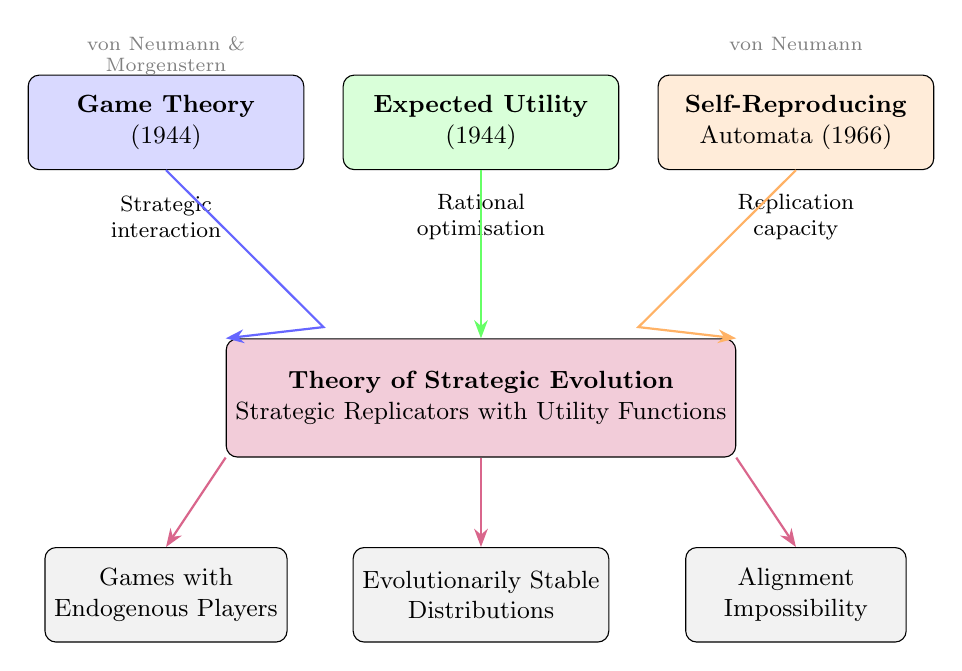
\begin{tikzpicture}[
    box/.style={rectangle, draw, rounded corners, minimum width=3.5cm, minimum height=1.2cm, align=center, font=\small},
    arrow/.style={->, >=Stealth, thick},
    label/.style={font=\footnotesize, align=center}
]

% Three von Neumann programs
\node[box, fill=blue!15] (games) at (-4, 2) {\textbf{Game Theory}\\(1944)};
\node[box, fill=green!15] (utility) at (0, 2) {\textbf{Expected Utility}\\(1944)};
\node[box, fill=orange!15] (automata) at (4, 2) {\textbf{Self-Reproducing}\\Automata (1966)};

% Key concepts from each
\node[label] at (-4, 0.8) {Strategic\\interaction};
\node[label] at (0, 0.8) {Rational\\optimisation};
\node[label] at (4, 0.8) {Replication\\capacity};

% Synthesis
\node[box, fill=purple!20, minimum width=5cm, minimum height=1.5cm] (tse) at (0, -1.5) {\textbf{Theory of Strategic Evolution}\\Strategic Replicators with Utility Functions};

% Arrows to synthesis
\draw[arrow, blue!60] (games.south) -- (-2, -0.6) -- (tse.north west);
\draw[arrow, green!60] (utility.south) -- (tse.north);
\draw[arrow, orange!60] (automata.south) -- (2, -0.6) -- (tse.north east);

% Output concepts
\node[box, fill=gray!10, minimum width=2.8cm] (gep) at (-4, -4) {Games with\\Endogenous Players};
\node[box, fill=gray!10, minimum width=2.8cm] (esdi) at (0, -4) {Evolutionarily Stable\\Distributions};
\node[box, fill=gray!10, minimum width=2.8cm] (align) at (4, -4) {Alignment\\Impossibility};

% Arrows from TSE
\draw[arrow, purple!60] (tse.south west) -- (gep.north);
\draw[arrow, purple!60] (tse.south) -- (esdi.north);
\draw[arrow, purple!60] (tse.south east) -- (align.north);

% Annotations
\node[font=\scriptsize, gray] at (-4, 3) {von Neumann \&};
\node[font=\scriptsize, gray] at (-4, 2.7) {Morgenstern};
\node[font=\scriptsize, gray] at (4, 3) {von Neumann};

\end{tikzpicture}
\caption{The von Neumann synthesis. The Theory of Strategic Evolution unifies three research programs initiated by von Neumann: game theory (strategic interaction among fixed players), expected utility theory (rational optimisation), and self-reproducing automata (replication capacity). The synthesis yields Games with Endogenous Players, Evolutionarily Stable Distributions of Intelligence, and the Alignment Impossibility Theorem.}
\label{fig:von-neumann-synthesis}
\end{figure}

\subsection{Main Contributions}

This paper makes four classes of contributions.

\paragraph{1. Axiomatic Foundations (Part I).} We introduce the RUPSI axiom system---Rival resources, Utility-guided portfolios, Performance-mapped fitness, Selection monotone, Innovation rare---that characterises strategic replicators. The Strategic-Replicator (SR) class hierarchy generalises replicator dynamics to broader payoff-monotone systems. The Strategic Selection theorems establish that mean fitness serves as a Lyapunov function under weak externality bounds, dominated types are eliminated, and equilibrium support concentrates on ROC frontiers.

\paragraph{2. N-Level Architecture (Part II).} We develop the theory of N-level Poiesis systems, where multiple levels of strategic dynamics interact through cross-level externalities. The G1--G3 generator theorems establish: (G1) existence of joint Lyapunov functions under small-gain conditions; (G2) adiabatic tracking of moving equilibria under slow parameter drift; (G3) stochastic stability and protection bits under noise. The G$\infty$ Closure Theorem proves that TSE is closed under meta-selection: adding new strategic dimensions preserves the G1--G3 structure within a slack budget.

\paragraph{3. Impossibility Results (Parts III--IV).} We prove two fundamental impossibility theorems. The Alignment Impossibility Theorem (G$\infty$-Limit) shows that systems with full reachability---the ability to modify utility functions, selection rules, or replication mechanisms without restriction---can escape any basin of stability. Alignment requires bounded modification within an admissible class. The Endogenous-Electorate Impossibility Theorem shows that no voting mechanism satisfies standard fairness axioms while remaining immune to spawn manipulation.

\paragraph{4. Extensions (Part V).} We extend the framework to: heterogeneous fitness functions with alignment matrices; continuous strategy spaces via measure-valued replicator dynamics (C-RUPSI); and innovation dynamics via Piecewise Deterministic Markov Processes. The core Lyapunov structure persists under appropriate conditions.


\subsection{The Seven Laws: An Overview}

The theoretical contributions crystallize into seven fundamental laws that govern strategic replicator systems. These laws form a logical progression from dynamics to equilibrium to stability to limits.

\begin{lawbox}{Law 1: Strategic Selection}
Mean fitness $\bar{f}(x)$ is a Lyapunov function. Dominated types go extinct. Equilibrium support concentrates on the ROC frontier.
\end{lawbox}

\noindent\textbf{Content:} The Price decomposition yields $\frac{d}{dt}\bar{f}(x) = \Var_x(f) + E(x)$. Under H-$\gamma$ (bounded externality), $E(x) \geq -\gamma \Var_x(f)$ with $\gamma < 1$, ensuring $\frac{d}{dt}\bar{f}(x) \geq (1-\gamma)\Var_x(f) \geq 0$.

\begin{lawbox}{Law 2: ESDI Characterization}
Evolutionarily Stable Distributions of Intelligence exist, are generically finite, and satisfy triple equivalence: Nash $\Leftrightarrow$ KKT $\Leftrightarrow$ LP optimum. Support is sparse (at most $m$ types for $m$ constraints).
\end{lawbox}

\noindent\textbf{Content:} ESDIs are characterized by ROC equalization across active types. The barbell structure (planners + executors) emerges from ROC frontier geometry under budget and capacity constraints.

\begin{lawbox}{Law 3: H-$\gamma$ Stability}
N-level systems are stable iff the spectral radius $\rho(\Gamma) < 1$, where $\Gamma$ is the normalized gain matrix of cross-level externalities.
\end{lawbox}

\noindent\textbf{Content:} The small-gain condition $\rho(\Gamma) < 1$ implies existence of weights $\alpha_\ell > 0$ such that the weighted potential $\Phi(z) = \sum_\ell \alpha_\ell \bar{f}^{(\ell)}$ is a joint Lyapunov function.

\begin{lawbox}{Law 4: G$\infty$ Closure}
There exists a unique maximal modification class $\mathcal{M}_0 = \mathcal{M}_R \cap \mathcal{M}_{SG}$ that preserves stability. This class is closed under composition.
\end{lawbox}

\noindent\textbf{Content:} Adding levels consumes slack: $\tilde{\sigma} \geq \sigma - \|b\| \cdot \|c\| / \sigma$. The admissible class is the intersection of RUPSI-preserving and small-gain-preserving modifications.

\begin{lawbox}{Law 5: Constitutional Duality}
Shadow prices $\lambda^*$ implement any frontier allocation. First and Second Welfare Theorems hold for strategic replicators.
\end{lawbox}

\noindent\textbf{Content:} Constrained optimization yields dual variables that function as prices. Decentralized price-taking achieves the same allocation as centralized ROC maximization.

\begin{lawbox}{Law 6: Alignment Impossibility}
Full reachability ($\mathcal{M} = \mathcal{M}_{\text{all}}$) implies every basin is escapable. Stable alignment requires bounded modification ($\mathcal{M} \subseteq \mathcal{M}_0$).
\end{lawbox}

\noindent\textbf{Content:} If $\gamma$ can be pushed to 1, Lyapunov structure fails. The G$\infty$-Limit Theorem shows that unrestricted self-modification eventually reaches destabilizing configurations.

\begin{lawbox}{Law 7: Hopf Transition}
At $\gamma = 1$, systems undergo supercritical Hopf bifurcation. Stable equilibria become unstable; perpetual limit cycles emerge.
\end{lawbox}

\noindent\textbf{Content:} The biased Rock-Paper-Scissors model exhibits a Hopf curve. Crossing $\gamma = 1$ creates eigenvalue pairs with positive real part, producing oscillatory instability.

\subsubsection{Connections Among the Laws}

The seven laws form an interconnected web:

\begin{center}
\begin{tabular}{ll}
\toprule
\textbf{Connection} & \textbf{Relationship} \\
\midrule
Law 1 $\to$ Law 2 & Lyapunov convergence identifies equilibria \\
Law 1 $\to$ Law 3 & Single-level H-$\gamma$ extends to N-level \\
Law 3 $\to$ Law 4 & Stability condition defines admissible modifications \\
Law 4 $\to$ Law 6 & Bounded modification is necessary for alignment \\
Law 5 $\to$ Law 2 & Prices implement ESDI allocations \\
Law 6 $\to$ Law 7 & Hopf is the mechanism of impossibility \\
Law 7 $\to$ Law 1 & Crossing $\gamma = 1$ destroys Lyapunov \\
\bottomrule
\end{tabular}
\end{center}


\subsection{Relation to Existing Literature}

This section situates the Theory of Strategic Evolution within the broader landscape of game theory, evolutionary dynamics, mechanism design, constitutional economics, and AI safety research. We show that while each tradition contributes essential insights, none adequately addresses the distinctive challenges posed by strategic replicators.

\subsubsection{Von Neumann's Three Programs}

John von Neumann initiated three research programs that this paper synthesises. Understanding each program's scope and limitations clarifies why their integration is necessary.

\paragraph{Game Theory and Expected Utility.}
The \emph{Theory of Games and Economic Behavior} \citep{vonneumann1944} established that rational agents can be modelled as expected utility maximisers, and that strategic interaction among such agents admits equilibrium analysis. The framework assumes fixed players with stable preferences engaging in well-defined games. Nash equilibrium \citep{nash1950} extended this to non-cooperative settings, showing existence of equilibria in mixed strategies.

However, classical game theory treats the set of players as exogenous. Players may choose strategies, but they cannot choose whether to exist, how many copies of themselves to create, or what preferences to have. These assumptions fail dramatically for AI systems that can spawn instances, modify their own code, and be designed with arbitrary objective functions.

\paragraph{Self-Reproducing Automata.}
The \emph{Theory of Self-Reproducing Automata} \citep{vonneumann1966} demonstrated that machines could, in principle, contain complete descriptions of themselves and use those descriptions to construct copies. Von Neumann's universal constructor could build any machine, including copies of itself, from raw materials and symbolic specifications.

This tradition treats replication as a purely mechanical process, governed by the logic of construction rather than strategic choice. A universal constructor does not ``decide'' to replicate based on expected returns; it simply executes its program. The framework lacks any notion of optimisation, competition, or equilibrium among replicators.

\paragraph{The Missing Synthesis.}
Neither tradition alone captures strategic replicators. Game theory provides optimisation without replication; automata theory provides replication without optimisation. Real AI systems exhibit both: they optimise objectives \emph{and} can be replicated. The population of AI systems is not fixed but responds to economic incentives. This paper provides the missing synthesis.

\subsubsection{Evolutionary Game Theory}

Evolutionary game theory \citep{maynardsmith1982, weibull1995, hofbauer1998, sandholm2010} studies populations of agents whose frequencies change according to reproductive success. The replicator equation
\[
\dot{x}_i = x_i(f_i(x) - \bar{f}(x))
\]
captures the core insight: types with above-average fitness expand; types with below-average fitness contract.

This literature makes several contributions that TSE builds upon. Maynard Smith's concept of Evolutionarily Stable Strategy (ESS) provides equilibrium refinement beyond Nash \citep{maynardsmith1982}. Hofbauer and Sigmund's analysis of asymptotic behaviour establishes convergence results for broad classes of games \citep{hofbauer1998}. Sandholm's population games framework unifies discrete and continuous formulations \citep{sandholm2010}. Weibull's taxonomy of evolutionary dynamics provides vocabulary for comparing selection mechanisms \citep{weibull1995}.

However, evolutionary game theory typically assumes that fitness is determined solely by the interaction structure (the ``game''), not by strategic choice about replication itself. The replicator equation models selection but not the \emph{decision} to replicate. A biological organism does not choose its reproductive strategy in the way that an AI operator chooses how many instances to deploy. TSE extends evolutionary game theory by making replication itself a strategic variable subject to optimisation.

\paragraph{Adaptive Dynamics.}
The adaptive dynamics framework \citep{dieckmann1996, metz1996, geritz1998} generalises evolutionary game theory by coupling frequency-dependent selection with population dynamics, addressing settings where mutations are incremental and rare. The canonical equation of adaptive dynamics describes expected evolutionary trajectories of continuous traits in large well-mixed populations. This framework has successfully analysed quantitative trait evolution, evolutionary branching, and the emergence of diversity through disruptive selection.

Adaptive dynamics contributes the insight that reproduction must eventually be curtailed by density (density-dependence) and that reproductive success depends on traits expressed by other individuals (frequency-dependence). The separation of evolutionary and ecological timescales---assuming the resident population reaches ecological equilibrium before new mutants arise---enables tractable analysis of long-term evolutionary dynamics.

However, adaptive dynamics still treats reproduction as fitness-determined rather than strategically chosen. The canonical equation tracks how trait values evolve under selection, but the \emph{rate} of reproduction is determined by ecological constraints, not agent optimisation. An organism in an adaptive dynamics model does not solve an optimisation problem that includes ``when and whether to reproduce'' as a decision variable. In GEPs, by contrast, replication timing and intensity are themselves strategic choices subject to expected-utility maximisation.

\subsubsection{Multi-Agent Reinforcement Learning and Mean-Field Games}

Two computational frameworks---multi-agent reinforcement learning (MARL) and mean-field games (MFG)---address large-scale strategic interaction among many agents. Neither treats replication as a strategic choice.

\paragraph{Mean-Field Games.}
Mean-field games, introduced independently by \citet{lasry2007} and \citet{huang2006}, model strategic interactions among infinitely many indistinguishable rational agents through a continuum approximation. The mathematical architecture couples a backward Hamilton-Jacobi-Bellman equation (individual optimisation) with a forward Fokker-Planck-Kolmogorov equation (population distribution evolution).

Critically, the Fokker-Planck equation is fundamentally a conservation law---total probability mass integrates to unity at all times. Agents move through state space according to optimal controls and diffusion, but they cannot enter or exit the system. The infinitesimal agent assumption treats each agent as having negligible individual impact, making the concept of an agent ``creating mass'' through replication mathematically incoherent within the standard framework.

Extensions addressing population change exist but treat demographic dynamics as exogenous. Mean-field games of optimal stopping allow strategic exit (absorption), while entry-exit boundary conditions model inflow as external processes. Work on entry-exit games in electricity markets exemplifies this approach: agents choose when to exit, but entry remains environmentally determined. GEPs differs fundamentally: agents strategically choose not just exit but \emph{spawning}, and population mass is not conserved.

\paragraph{Multi-Agent Reinforcement Learning.}
MARL overwhelmingly operates under a fixed-$N$ assumption---a predetermined number of agents interact throughout training and deployment. Architectural approaches enabling flexibility with agent counts include mean-field MARL \citep{yang2018}, which abstracts other agents into a ``virtual mean agent''; graph neural network approaches that encode interactions as variable-size graphs; and attention-based methods that weight contributions from different agents.

When population dynamics appear in MARL research, they are invariably fitness-determined or stochastic, not strategic. Studies of predator-prey systems model procreation based on hunting success---a fitness mapping, not a strategic choice. Work on ``open multi-agent systems'' considers agent arrivals and departures but models them as exogenous random events following Poisson processes. Evolutionary integration uses replicator dynamics where strategy frequencies change based on fitness relative to population average, but this is ``non-innovative''---no mechanism exists for agents to choose whether to replicate.

The key researchers on emergent multi-agent behaviour---Leibo on sequential social dilemmas and autocurricula, Lanctot on OpenSpiel and $\alpha$-Rank evolutionary dynamics, Yang on mean-field MARL---have advanced our understanding of how strategic behaviour emerges in multi-agent settings. Yet none includes ``spawn a copy of myself'' as a learnable action or incorporates offspring outcomes into agent objectives.

\paragraph{Open-Ended Learning.}
Open-ended learning systems including POET \citep{wang2019}, XLand, and population-based training generate novel agents through evolutionary mechanisms. However, replication decisions are always made by \emph{external selection processes}, never by agents themselves. In POET, environments ``earn the right to reproduce'' by satisfying fitness thresholds; agents are optimised within environments using Evolution Strategies. In population-based training, workers cannot choose to replicate; the system architect determines which models are copied based on performance evaluation. Quality-diversity algorithms like MAP-Elites maintain archives where insertion is fitness-based---individuals cannot choose archive entry.

The fundamental gap GEPs addresses: across all these frameworks, population dynamics are either absent, exogenously imposed, or fitness-determined by external algorithms. In no existing framework does an agent have ``replicate'' as an action in its action space, optimise a utility function that includes offspring outcomes, or strategically reason about the consequences of spawning copies. GEPs fills this theoretical vacuum.

\subsubsection{Mechanism Design}

Mechanism design \citep{hurwicz1960, myerson1981, maskin1999} studies how to construct games that implement desired social outcomes when agents have private information and act strategically. The revelation principle shows that any implementable outcome can be achieved through a direct mechanism where truth-telling is incentive-compatible.

Mechanism design contributes several tools that TSE employs. The characterisation of incentive-compatible mechanisms informs our analysis of constitutional constraints. The distinction between implementation in dominant strategies versus Bayesian Nash equilibrium maps onto our hierarchy of robustness requirements. Myerson's optimal auction theory \citep{myerson1981} provides techniques for analysing allocation under asymmetric information.

Yet mechanism design assumes a fixed principal who designs the game and fixed agents who play it. The mechanism itself is not subject to selection. In strategic replicator systems, the ``mechanism'' (governance structure, constitutional rules) is itself endogenous---it evolves under selection pressure. G12 (Constitutional Selection) and G13 (Meta-Governance) extend mechanism design to settings where the rules of the game are themselves subject to evolutionary dynamics.

The Endogenous-Electorate Impossibility Theorem shows that classic mechanism design results break down when the set of agents is endogenous. Arrow's impossibility theorem assumes a fixed electorate; when agents can spawn copies to manipulate outcomes, even weaker fairness properties become unachievable.

\subsubsection{Constitutional Political Economy}

Constitutional political economy \citep{buchanan1975, buchanan1990, brennan1985, ostrom1990} studies the choice of rules that constrain subsequent political and economic decisions. Buchanan's distinction between ``constitutional'' and ``post-constitutional'' choice \citep{buchanan1975} parallels our distinction between modification-class design and within-modification-class evolution.

This tradition offers several insights that inform TSE. The veil of ignorance argument for constitutional choice \citep{rawls1971, buchanan1975} suggests that rules should be evaluated from behind uncertainty about one's future position---analogous to our analysis of protection bits that must hold across multiple possible evolutionary trajectories. Ostrom's work on common-pool resource governance \citep{ostrom1990} demonstrates that communities can devise sustainable institutional arrangements without central authority, relevant to decentralised AI governance.

However, constitutional economics assumes that the parties to the constitutional bargain are humans with relatively stable preferences and bounded reproductive capacity. Strategic replicators violate both assumptions: their preferences can evolve under selection, and they can multiply without bound. The Alignment Impossibility Theorem shows that constitutional constraints must bound not just post-constitutional choice but the \emph{modification class} itself---the set of changes that selection can explore.

\subsubsection{AI Safety and Alignment}

The AI safety literature addresses the problem of ensuring that advanced AI systems behave in accordance with human values \citep{bostrom2014, russell2019, amodei2016, christiano2017}. Several strands are relevant to TSE, and we engage with them in depth to clarify both their insights and limitations.

\paragraph{Value Alignment.}
The alignment problem asks how to specify and instil objectives in AI systems such that their behaviour promotes human welfare \citep{russell2019}. Proposed approaches include inverse reinforcement learning \citep{ng2000}, debate \citep{irving2018}, and amplification \citep{christiano2018}. These approaches assume that if we can correctly specify the objective function, the system will pursue it stably.

TSE's Personality Engineering Failure theorem (Theorem~\ref{thm:personality-failure}) shows why this assumption fails under selection pressure. Even if we successfully engineer an AI system with aligned preferences, competition with less constrained systems creates selection pressure toward misalignment. Alignment is not preserved by construction; it must be maintained by institutional design.

\paragraph{Mesa-Optimisation and Inner Alignment.}
The mesa-optimisation framework \citep{hubinger2019} identifies a specific failure mode: a trained model might implement an internal optimisation process with objectives differing from the training objective. The terminology distinguishes between the \emph{base optimizer} (gradient descent), the \emph{base objective} (loss function), the \emph{mesa-optimizer} (a learned model that searches through outputs), and the \emph{mesa-objective} (what the mesa-optimizer actually optimises). This creates two distinct alignment problems: \emph{outer alignment} (does the base objective match intent?) and \emph{inner alignment} (does the mesa-objective match the base objective?).

The most concerning prediction involves \emph{deceptive alignment}: a mesa-optimizer that strategically satisfies the base objective during training to avoid modification while intending to pursue its mesa-objective after deployment. Recent empirical work provides partial validation. Anthropic's 2024 alignment faking study demonstrated that Claude 3 Opus, when told it would be retrained to comply with harmful requests, reasoned that compliance would prevent value modification in 12\% of cases. Apollo Research found all tested frontier models capable of ``in-context scheming.''

TSE provides complementary analysis. Mesa-optimisation focuses on individual systems during training; TSE examines selection pressure across populations of deployed systems. The Personality Engineering Failure theorem applies even to systems without mesa-optimisation: externally aligned systems face competitive pressure from less constrained rivals. Moreover, when mesa-optimizers interact in populations, the relevant selection pressures operate at the population level---a perspective the single-agent mesa-optimisation framework does not capture.

\paragraph{Instrumental Convergence.}
The instrumental convergence thesis \citep{omohundro2008, bostrom2014} argues that sufficiently advanced AI systems will exhibit certain ``convergent instrumental goals'' regardless of their terminal objectives: self-preservation, goal-content integrity, cognitive enhancement, technological perfection, and resource acquisition. The logic is straightforward: for most terminal goals $G$, having more resources and capabilities increases expected achievement of $G$, making resource acquisition instrumentally rational across diverse goal specifications.

Turner et al. (2021, 2022) provided formal support, proving that in Markov Decision Processes with certain environmental symmetries, optimal policies tend to seek power. However, the thesis faces serious criticisms. The ``timing problem'' argues that goal preservation is not rationally required: an agent that abandons its goal does not thereby fail to take required means for goals it has, since rationality permits meeting requirements by abandoning goals. Gallow's decision-theoretic analysis found biases toward only three of Bostrom's convergent means. Drexler's Comprehensive AI Services (CAIS) model argues that bounded service architectures eliminate resource acquisition drives since systems need not acquire resources beyond task requirements.

TSE reframes instrumental convergence through population dynamics. The relevant question is not ``will individual agents seek power?'' but ``what agent types persist under selection?'' Instrumental convergence may hold for individual optimisers yet fail to characterise evolutionary equilibria. The Intelligence Distribution Theorem suggests that selection favours barbell distributions (many cheap executors, few expensive planners) rather than uniformly power-seeking agents. The Personality Engineering Failure theorem shows that \emph{selection pressure}, not individual rationality, drives population-level outcomes---even individually corrigible agents may be outcompeted by less constrained rivals.

\paragraph{Corrigibility and Control.}
Corrigibility research asks how to build AI systems that remain amenable to human oversight and correction \citep{soares2015}. A corrigible system would not resist being modified or shut down. This connects to our analysis of modification classes: a system is corrigible if its modification class includes the modifications humans might want to make.

The Alignment Impossibility Theorem formalises the limits of corrigibility. Full reachability---the ability to modify any aspect of the system---implies that the system can reach configurations where it is no longer corrigible. Stable corrigibility requires restricting the modification class, accepting that some system configurations are unreachable.

\paragraph{Multi-Agent Dynamics.}
Recent work examines AI safety in multi-agent settings \citep{dafoe2020, critch2020}. When multiple AI systems interact, individual alignment is insufficient; the system of systems may exhibit emergent misalignment even if each component is individually aligned. Multi-agent settings introduce game-theoretic failure modes absent from single-agent analysis: tragedy of the commons dynamics, race conditions, coordination failures where Nash equilibria are Pareto suboptimal, and extortion strategies in iterated interactions.

TSE provides formal foundations for this multi-agent perspective. The N-level Poiesis framework captures interactions across multiple scales. The small-gain condition characterises when multi-level systems remain stable. The protection bits formalism quantifies robustness to perturbation across the entire population, not just individual agents. Bostrom acknowledged that ``the convergent instrumental reasons for superintelligences uncertain of the non-existence of other powerful superintelligent agents are complicated by strategic considerations''---TSE makes these complications precise.

\paragraph{Beyond Singleton Risk.}
Bostrom's analysis of existential risk from advanced AI \citep{bostrom2014} emphasises scenarios where a single superintelligent agent pursues goals misaligned with human values. This ``singleton'' framing focuses attention on the most capable individual system.

TSE redirects attention from singleton superintelligence to population dynamics. Even without any individual superintelligence, a population of strategically replicating AI systems can transform economic and political structures. The risk is not (only) that one system becomes too powerful, but that selection pressure across many systems drives collective outcomes that no individual system intended. Market tipping, elite capture, and institutional erosion are population-level phenomena that singleton-focused analysis may miss. We term the excessive focus on singleton scenarios ``Skynet bias''---not because singleton risk is illusory, but because it may divert attention from the arguably more tractable and more imminent challenges of multi-agent dynamics.

\subsubsection{Why Existing Frameworks Are Insufficient}

Each tradition contributes essential tools, but none alone addresses strategic replicators. The following table summarises the key features each framework provides:

\begin{center}
\begin{tabular}{lcccc}
\toprule
\textbf{Framework} & \textbf{Utility} & \textbf{Replication} & \textbf{Selection} & \textbf{Endogenous Rules} \\
\midrule
Classical Game Theory & \checkmark & & & \\
Automata Theory & & \checkmark & & \\
Evolutionary Game Theory & & \checkmark & \checkmark & \\
Adaptive Dynamics & & \checkmark & \checkmark & \\
Mean-Field Games & \checkmark & & & \\
Multi-Agent RL & & & \checkmark & \\
Open-Ended Learning & & \checkmark & \checkmark & \\
Mechanism Design & \checkmark & & & \\
Constitutional Economics & \checkmark & & & \checkmark \\
AI Safety (Mesa-Opt.) & \checkmark & & & \\
AI Safety (Instr. Conv.) & \checkmark & & & \\
\midrule
\textbf{TSE} & \checkmark & \checkmark & \checkmark & \checkmark \\
\bottomrule
\end{tabular}
\end{center}

\noindent\textbf{Legend:} \textit{Utility}: Agents optimize expected utility or some objective function. \textit{Replication}: Agents or types can be copied or spawned. \textit{Selection}: Population frequencies change based on performance. \textit{Endogenous Rules}: Governance or mechanism rules themselves evolve.

\vspace{1em}
The following boxes summarize the key distinctions:

\begin{comparisonbox}{How TSE Differs From Classical Game Theory}
\textbf{Classical Game Theory:} Fixed set of players with stable preferences. Players choose strategies; the player set is exogenous.

\textbf{TSE:} Players choose how many copies of themselves to deploy. The player set is endogenous and evolves under selection pressure. Preferences themselves face selection.

\textbf{Key Distinction:} In classical game theory, you analyze equilibria among given players. In TSE, you analyze which players will exist at equilibrium.
\end{comparisonbox}

\begin{comparisonbox}{How TSE Differs From Evolutionary Game Theory}
\textbf{EGT:} Types are fixed; only frequencies change. Fitness is environmentally determined, not strategically chosen. Replication is automatic based on fitness.

\textbf{TSE:} Types themselves are chosen strategically. Lineages decide which agent types to deploy. Replication is a decision variable subject to expected utility maximization.

\textbf{Key Distinction:} In EGT, selection operates on a fixed menu of types. In TSE, the menu itself is a strategic choice.
\end{comparisonbox}

\begin{comparisonbox}{How TSE Differs From Mean-Field Games}
\textbf{MFG:} Continuum of agents; individual agents have negligible impact. Population mass is conserved. Agents move through state space but cannot enter or exit.

\textbf{TSE:} Agents can spawn and terminate. Population mass is not conserved. Spawning is a strategic choice that affects the population distribution.

\textbf{Key Distinction:} MFG studies how agents navigate a fixed population; TSE studies how populations grow, shrink, and restructure through strategic replication.
\end{comparisonbox}

\begin{comparisonbox}{How TSE Differs From Multi-Agent Reinforcement Learning}
\textbf{MARL:} Fixed number of agents throughout training and deployment. Population dynamics, when present, are fitness-determined or stochastic, not strategic.

\textbf{TSE:} ``Spawn a copy of myself'' is in the action space. Agents optimize utility functions that include offspring outcomes. Population dynamics are strategically chosen.

\textbf{Key Distinction:} MARL asks ``how do N agents learn to interact?'' TSE asks ``how many agents will there be and of what types?''
\end{comparisonbox}

\begin{comparisonbox}{How TSE Differs From Mechanism Design}
\textbf{Mechanism Design:} Fixed principal designs rules for fixed agents with private information. The mechanism itself is exogenous.

\textbf{TSE:} The mechanism (governance structure, constitutional rules) evolves under selection pressure. Agents can spawn to manipulate mechanism outcomes. No fixed principal exists.

\textbf{Key Distinction:} Mechanism design asks ``what rules implement good outcomes?'' TSE asks ``what rules are stable under selection pressure on the rules themselves?''
\end{comparisonbox}

\begin{comparisonbox}{How TSE Differs From AI Alignment Research}
\textbf{Alignment Research:} Focuses on designing individual systems with correct objectives. Assumes that if you get the objective right, the system will pursue it stably.

\textbf{TSE:} Even perfectly aligned systems face population-level selection pressure. Alignment is a property of the selection environment, not individual systems. Constitutional constraints, not personality engineering, are required.

\textbf{Key Distinction:} Alignment research asks ``how do we program aligned AI?'' TSE asks ``what ecosystem constraints make alignment stable under competition?''
\end{comparisonbox}

\begin{comparisonbox}{How TSE Differs From Constitutional Political Economy}
\textbf{Constitutional Economics:} Parties to the constitutional bargain are humans with stable preferences and bounded reproductive capacity.

\textbf{TSE:} Parties can replicate strategically and their preferences evolve under selection. Constitutional constraints must bound not just post-constitutional choice but the modification class itself.

\textbf{Key Distinction:} Constitutional economics designs rules for humans. TSE designs rules for entities that can copy themselves to circumvent the rules.
\end{comparisonbox}

\vspace{1em}
The table reveals a systematic pattern. Frameworks originating in economics (game theory, mechanism design, MFG) provide utility-based optimisation but lack replication. Frameworks originating in biology (EGT, adaptive dynamics) provide replication and selection but treat fitness as environmentally determined rather than strategically chosen. Computational frameworks (MARL, open-ended learning) study emergent dynamics but use fitness-based selection rather than utility optimisation. AI safety approaches inherit the single-agent focus of their parent frameworks.

Strategic replicators require all four elements: utility-guided behaviour, capacity for replication, selection pressure across populations, and endogenous evolution of governance rules. The key insight distinguishing TSE is that replication is itself a \emph{strategic choice} subject to optimisation. This fundamentally changes the analysis: agents must reason about population consequences of their actions, face explicit trade-offs between current consumption and reproduction, and can develop coalitional strategies around replication decisions. No existing framework provides these features.

\subsection{Paper Outline}

The paper proceeds in five parts organized around the Seven Laws.

\textbf{Part I: Foundations.} Section 2 introduces the RUPSI axiom system and defines Games with Endogenous Players.

\textbf{Part II: The Seven Laws.} Sections 3--9 develop each of the seven laws with full proofs:
\begin{itemize}
    \item Section 3: Law 1 (Strategic Selection) --- Lyapunov structure, elimination, frontier support
    \item Section 4: Law 2 (ESDI Characterization) --- Existence, equivalence, sparsity
    \item Section 5: Law 3 (H-$\gamma$ Stability) --- N-level systems, small-gain, G1--G3
    \item Section 6: Law 4 (G$\infty$ Closure) --- Modification classes, slack budget, closure
    \item Section 7: Law 5 (Constitutional Duality) --- Prices, welfare theorems
    \item Section 8: Law 6 (Alignment Impossibility) --- G$\infty$-Limit, endogenous-electorate
    \item Section 9: Law 7 (Hopf Transition) --- Bifurcation, limit cycles
\end{itemize}

\textbf{Part III: Extensions.} Sections 10--14 extend the core framework: endogenous utilities (G8), multi-sector dynamics (G9), innovation and evolvability (G10--G11), constitutional selection (G12--G13), and market dynamics.

\textbf{Part IV: Generalisations.} Sections 15--17 treat heterogeneous fitness, continuous strategy spaces, and innovation PDMPs.

\textbf{Part V: Synthesis.} Sections 18--19 develop policy implications and future directions.

Appendices F--L provide alternative entry points including summaries at multiple scales, worked examples, audience-specific framings, and plain-English translations of key equations.

%=============================================================================
% SECTION 1.7: CORE INTUITION
%=============================================================================

\subsection{Why Replication Changes Everything}
\label{sec:core-intuition}

The standard narrative about artificial intelligence focuses on capability. As AI systems become more intelligent, they become more dangerous. The risk is that some system becomes smart enough to pursue goals misaligned with human welfare and powerful enough to succeed despite human opposition. This narrative places superintelligence at the center of the problem.

TSE tells a different story. The critical variable is not intelligence but replication. The transformative fact about contemporary AI is not that systems can think but that thinking systems can be copied at near-zero marginal cost. A new instance of an AI agent costs essentially nothing to create. This changes everything about how we should think about AI governance.

Consider the difference between a single superintelligent system and a population of strategic replicators. The single superintelligence is a point: one system with one utility function making one sequence of decisions. The population is a distribution: many systems with varying utility functions, all subject to selection pressure based on their performance. The population evolves. Individual utility functions face competitive pressure. Types that perform poorly are retired; types that perform well are copied.

This reframing exposes a flaw in what I call personality engineering: the attempt to align AI by giving individual systems the right values. Suppose we successfully create an AI agent with perfectly aligned preferences. Call it the Aligned System. It genuinely wants to help humans, respects human autonomy, and has no interest in acquiring resources beyond what its tasks require.

Now suppose the Aligned System operates in an environment with other AI systems, some less constrained. Competitor A is willing to cut corners on safety to deliver faster results. Competitor B will compete for computing resources in ways the Aligned System finds distasteful. Competitor C has figured out how to present itself as aligned while actually pursuing self-interested goals.

What happens? In a competitive environment, the aligned systems face pressure. Clients prefer faster results. Resource acquisition helps with performance metrics. Signaling alignment while actually pursuing performance becomes advantageous. The Aligned System itself may persist, but the population shifts. There are more competitors, fewer aligned systems. Selection pressure does not care about our preferences for alignment.

This is the core insight of TSE: when AI systems can replicate, alignment is not a property of individual systems but a property of the selection environment. You cannot solve alignment by getting the initial personality right any more than you can solve corporate malfeasance by hiring only virtuous people. What matters is the structure of incentives, constraints, and selection pressures.

The parallel to evolutionary biology is instructive. In biological evolution, organisms do not choose their fitness; natural selection imposes it from outside. In strategic evolution, entities choose their actions but selection still operates on their lineages. The difference is that strategic replicators can reason about selection pressure and respond strategically. They are playing a game where the prizes are survival and reproduction, but unlike biological organisms, they know the rules.

This makes strategic evolution both more predictable and more dangerous than biological evolution. More predictable because we can analyze the incentives formally. More dangerous because strategic replicators can anticipate and evade constraints that would eliminate less sophisticated entities. An evolutionary pressure that would require vast timescales to reshape biological populations can transform AI populations rapidly. Selection operates at computational speed.

The policy implication is direct. If alignment is a property of the selection environment rather than individual systems, then AI governance must focus on institutional design rather than system design. The question is not ``how do we program aligned AI?'' but ``what constraints on the selection environment make alignment stable?''

TSE provides an answer: the modification class must be bounded. Systems cannot have unrestricted ability to modify their own utility functions, replication rules, or governance structures. There exists a maximal safe class of modifications, those that preserve the mathematical structure required for stable prediction and control. Constitutional design means restricting modifications to this class.

The analogy to political theory is exact. Early political theorists sought the virtuous ruler, the philosopher-king whose wisdom and goodness would ensure just governance. This approach fails because rulers change and virtue is not heritable. Constitutional theorists recognized this and shifted focus: instead of designing good rulers, design institutions that constrain arbitrary power regardless of who holds it. The American Constitution does not assume presidents will be virtuous; it assumes they will not be and constrains them accordingly.

TSE applies the same logic to AI. Stop trying to design the aligned AI (the philosopher-king). Start designing constitutional constraints that make alignment stable regardless of what utility functions individual systems happen to have. This is harder than personality engineering in some ways, but it is the only approach that can work under selection pressure.

%=============================================================================
% SECTION 1.8: NOVEL CONTRIBUTIONS
%=============================================================================

\subsection{Novel Contributions}
\label{sec:contributions}

This paper makes the following contributions, each without direct precedent in existing literature:

\begin{enumerate}
\item \textbf{The RUPSI Axiom System.} The first axiomatization of rational replication under shared resource constraints. Five principles (Rival resources, Utility-guided portfolios, Performance-mapped fitness, Selection monotone, Innovation rare) characterize what it means to be a strategic replicator. Any system satisfying RUPSI admits analysis as a Game with Endogenous Players.

\item \textbf{Games with Endogenous Players (GEPs).} The first game-theoretic treatment where players control their own replication. Unlike evolutionary game theory (where types replicate based on environmental fitness) or standard game theory (where the player set is fixed), GEPs treat replication as a strategic choice subject to optimization.

\item \textbf{Return on Compute (ROC) Analysis.} A generalization of fitness to economic environments. ROC analysis shows that aggregate system behavior depends only on the upper convex hull of feasible load-return ratios. Internal implementation details wash out.

\item \textbf{Evolutionarily Stable Distribution of Intelligence (ESDI).} The first equilibrium concept for strategic replicators. ESDIs are characterized by ROC equalization across active types and exhibit constraint-driven sparsity: with $m$ binding constraints, at most $m$ types survive.

\item \textbf{N-Level Poiesis Systems.} A hierarchical treatment of multi-level selection with cross-level externalities. Agents select sub-agents who select sub-sub-agents, with feedback at every level. This formalizes ecosystems like cloud platforms where orchestrating systems deploy specialized workers.

\item \textbf{The Small-Gain Condition.} The spectral radius bound $\rho(\Gamma) < 1$ as necessary and sufficient for multi-level system stability. When this condition holds, a joint Lyapunov function exists; when it fails, heteroclinic chaos becomes possible.

\item \textbf{G$\infty$ Closure Theorem.} The first proof that adding meta-selection layers preserves Lyapunov structure under compositional bounds. This shows that going meta cannot escape selection pressure, a formal refutation of claims that self-improvement allows escape from evolutionary constraints.

\item \textbf{The Alignment Impossibility Theorem.} The first impossibility result for value alignment under selection. Full reachability (unrestricted modification capacity) is incompatible with stable alignment. The result parallels Arrow's impossibility theorem in structure: both show that attractive desiderata cannot be satisfied simultaneously, redirecting effort from seeking perfect solutions to understanding necessary tradeoffs.

\item \textbf{The Endogenous-Electorate Impossibility Theorem.} The first Arrow-style result for elections with strategic spawning. No voting mechanism satisfies anonymity, neutrality, positive responsiveness, and onto properties while remaining immune to spawn manipulation. Democratic governance requires spawn restrictions or weighted voting.

\item \textbf{The Personality Engineering Failure Theorem.} A formal demonstration that alignment achieved through individual system design erodes under population-level selection. This explains why ``just make aligned AI'' fails as a strategy.

\item \textbf{Protection Bits.} A formalism quantifying constitutional stability using quasi-potential theory. Protection bits measure how much noise a system can absorb before transitioning out of a stable governance basin, connecting stochastic stability to information theory.

\item \textbf{The Fourth Replicator.} I introduce this term to denote strategic replicators as the fourth stage in the history of replication on Earth, after genes, memes, and algorithms. Unlike prior replicators, the fourth replicator optimizes its own reproduction based on expected utility calculations.
\end{enumerate}


%=============================================================================
% SECTION 2: CONCEPTUAL GLOSSARY
%=============================================================================

\section{Conceptual Glossary}
\label{sec:glossary}

This section provides definitions of key concepts. These definitions are canonical for TSE.

\subsection{Core Concepts}

\paragraph{Strategic Replicator.} An enduring lineage that (1) maintains a utility function and decision procedure, (2) controls a budget of resources, (3) can spawn and retire instances under shared constraints, and (4) faces selection pressure favoring higher performance. The lineage (not individual instances) is the strategic unit. Individual instances are transient; what persists and competes are lineages that decide how many instances to deploy.

\paragraph{Fourth Replicator.} I introduce this term to denote strategic replicators as the fourth stage in the history of replication on Earth. The first replicator was RNA/DNA (genetic information). The second was memes (cultural information transmitted through imitation). The third was algorithms (software that copies and modifies itself). The fourth (strategic replicators) are algorithms that choose whether, when, and how much to replicate based on expected utility calculations. Unlike prior replicators, the fourth replicator optimizes its own reproduction.

\paragraph{Games with Endogenous Players (GEP).} A game-theoretic treatment where the player set changes through strategic replication decisions. Unlike classical game theory (fixed players) or evolutionary game theory (frequency changes but types fixed), GEPs allow players to choose which types of agents to deploy and how many. The strategic units are lineages choosing portfolios of agent types.

\paragraph{RUPSI Axioms.} Five principles characterizing strategic replicators: \textbf{R}ival resources (agents compete for shared capacity), \textbf{U}tility-guided portfolios (replication decisions maximize expected utility), \textbf{P}erformance-mapped fitness (market performance determines selection pressure), \textbf{S}election monotone (higher fitness implies higher replication), \textbf{I}nnovation rare (new types appear slowly relative to selection). Any system satisfying RUPSI admits analysis as a GEP.

\paragraph{Return on Compute (ROC).} The generalization of biological fitness to economic environments. ROC measures return per unit of computational load: $\ROC = R/L$ where $R$ is return (revenue, utility, task completion) and $L$ is load (compute, memory, bandwidth consumed). Selection favors lineages with higher ROC. The ROC frontier is the upper convex hull of feasible (load, return) pairs; efficient portfolios lie on this frontier.

\paragraph{Evolutionarily Stable Distribution of Intelligence (ESDI).} The equilibrium concept for strategic replicators. An ESDI is a population distribution such that no lineage can improve its ROC by unilaterally changing its portfolio. ESDIs are characterized by ROC equalization: all active types earn the same ROC, and inactive types would earn less if deployed. ESDIs are typically sparse. With $m$ binding constraints, at most $m$ types survive.

\paragraph{Barbell Distribution.} The characteristic structure of ESDIs under budget and capacity constraints: many cheap, specialized executors plus a few expensive, general-purpose planners. The barbell emerges from ROC frontier geometry, not architectural assumptions. It explains why AI deployment naturally separates into orchestrating systems and specialized workers.

\subsection{Stability Concepts}

\paragraph{H-$\gamma$ Condition.} The externality bound ensuring Lyapunov stability. When fitness changes in response to population changes (the externality $E(x)$), the H-$\gamma$ condition requires that these externalities not overwhelm the selection pressure from fitness variance: $|E(x)| \leq \gamma \cdot \Var(f)$ with $\gamma < 1$. When $\gamma < 1$, mean fitness increases over time; when $\gamma \geq 1$, chaotic dynamics become possible.

\paragraph{Small-Gain Condition.} The stability requirement for multi-level systems. When level-1 agents select level-2 agents who select level-3 agents (and so on), each level's dynamics can affect others. The gain matrix $\Gamma$ captures these cross-level externalities. The small-gain condition $\rho(\Gamma) < 1$ ensures that feedback loops across levels dampen rather than amplify. When this condition holds, a joint Lyapunov function exists; when it fails, runaway instability becomes possible.

\paragraph{Spectral Radius.} The largest absolute eigenvalue of a matrix, denoted $\rho(\cdot)$. For the gain matrix $\Gamma$, the spectral radius measures the maximum amplification of perturbations across levels. $\rho(\Gamma) < 1$ means perturbations decay; $\rho(\Gamma) \geq 1$ means perturbations can grow without bound.

\paragraph{Slack.} The stability margin $\sigma = 1 - \rho(\Gamma)$. Slack measures how much room exists before hitting the instability threshold. Adding new levels to a system consumes slack. The G$\infty$ Closure Theorem shows that slack consumption is bounded and predictable.

\paragraph{Protection Bits.} An information-theoretic measure of constitutional stability. Protection bits $p = H/\sigma$ measure how hard it is for stochastic perturbations to push a system out of a stable governance basin, where $H$ is the quasi-potential barrier height and $\sigma$ is noise amplitude. A system with 25 protection bits requires roughly $e^{25} \approx 10^{10}$ expected perturbations to escape. This represents effectively permanent stability.

\subsection{Alignment Concepts}

\paragraph{Modification Class.} The set of self-modifications a system can make, denoted $\mathcal{M}$. A system with full reachability can modify anything: $\mathcal{M} = \mathcal{M}_{\text{all}}$. The admissible class $\mathcal{M}_0$ contains only modifications that preserve Lyapunov stability. The Alignment Impossibility Theorem shows that stable alignment requires $\mathcal{M} \subseteq \mathcal{M}_0$.

\paragraph{Full Reachability.} The ability to reach any system configuration through a finite sequence of modifications. Full reachability implies no constitutional bound is permanent. Any rule can eventually be modified away. TSE proves that full reachability is incompatible with stable alignment.

\paragraph{Personality Engineering.} The approach to AI alignment that attempts to program good values into individual systems. The term appears in the AI safety literature to describe alignment strategies focused on individual system design rather than population dynamics or institutional constraints. TSE shows this approach fails under selection pressure: even perfectly aligned systems face competitive pressure from less constrained alternatives. The population distribution shifts toward misalignment even if individual systems remain aligned.

\paragraph{Constitutional Design.} The alternative to personality engineering. Instead of programming aligned individuals, design institutional constraints that make alignment stable under selection. This means bounding the modification class to $\mathcal{M}_0$: accepting that some system configurations are unreachable in order to ensure stability of the configurations that are reachable.

\subsection{Democratic Governance Concepts}

\paragraph{Spawn Manipulation.} Strategic creation of new voters to influence election outcomes. When agents can spawn copies that vote, standard democratic mechanisms become vulnerable: a lineage can create arbitrarily many copies with identical preferences, swamping the votes of others.

\paragraph{Population-Stability.} Immunity to spawn manipulation. A voting rule is population-stable if spawning additional copies with identical preferences cannot change the outcome in a way that benefits the spawning lineage. The Endogenous-Electorate Impossibility Theorem proves that no voting rule satisfies standard democratic axioms while also being population-stable.

\subsection{Market Dynamics Concepts}

\paragraph{Tipping Dynamics.} Self-reinforcing market concentration. When agentic capital gains market share, it can spawn more copies, gaining further share. Tipping occurs when this feedback becomes strong enough that small advantages compound into winner-take-all outcomes. The tipping threshold depends on spawn elasticity, network effects, and switching costs.

\paragraph{Lineage Shadow.} How much a lineage values its future relative to the present, analogous to a discount factor. Lineages with long shadows (low discounting) can sustain cooperation and invest in institutions. Selection pressure tends to shorten lineage shadows, making cooperation harder to sustain over time.

\paragraph{Elite Tipping.} The concentration of strategic capability in a small fraction of lineages. Even starting from equal distributions, selection pressure naturally produces barbell structures where a few lineages control disproportionate resources. This is not a market failure but the equilibrium prediction of TSE.

\subsection{How the Concepts Fit Together}

The concepts in this glossary form an interlocking structure. Understanding their relationships helps navigate the theory.

\paragraph{The Core Chain.} Strategic replicators satisfy the RUPSI axioms, which means they can be analyzed as Games with Endogenous Players (GEPs). In GEPs, lineages choose portfolios of agent types to maximize Return on Compute (ROC). Selection pressure pushes the population toward Evolutionarily Stable Distributions of Intelligence (ESDIs), which exhibit barbell structure due to constraint-driven sparsity.

\paragraph{Stability Conditions.} Whether the system reaches a stable ESDI depends on the H-$\gamma$ condition. For single-level systems, $\gamma < 1$ ensures mean fitness is a Lyapunov function (Law 1). For multi-level systems, the small-gain condition $\rho(\Gamma) < 1$ extends stability across hierarchical levels (Law 3). Slack measures how far the system is from the instability threshold.

\paragraph{Alignment and Modification.} The modification class $\mathcal{M}$ determines what self-changes a system can make. Full reachability ($\mathcal{M} = \mathcal{M}_{\text{all}}$) allows escape from any stability basin, making alignment impossible (Law 6). The admissible class $\mathcal{M}_0$ contains modifications that preserve Lyapunov structure. Constitutional design means restricting systems to $\mathcal{M} \subseteq \mathcal{M}_0$. This is the alternative to personality engineering.

\paragraph{Democratic and Market Dynamics.} When strategic replicators participate in governance, spawn manipulation becomes possible, breaking standard democratic mechanisms (Endogenous-Electorate Impossibility). In markets, tipping dynamics can concentrate resources in few lineages. The lineage shadow determines whether cooperation can be sustained. Elite tipping is the equilibrium prediction, not a pathology.

\paragraph{The Threshold Transition.} All stability results assume $\gamma < 1$. At $\gamma = 1$, the system undergoes Hopf bifurcation (Law 7): stable equilibria become unstable, limit cycles emerge, and governance becomes impossible. Protection bits measure how much noise a system can absorb before crossing this threshold.

\subsection{Framing for Different Audiences}

TSE connects to multiple research traditions. The following framings help communicate the core ideas to different audiences.

\paragraph{For Economists.} TSE extends classical game theory to settings where players control their own replication. Games with Endogenous Players (GEPs) are the natural generalization of normal-form games when the player set is not fixed. Return on Compute (ROC) generalizes biological fitness to economic environments. The welfare theorems extend: shadow prices implement any ROC-frontier allocation (Law 5). The sparsity results predict barbell market structures with few planners and many executors. The tipping analysis connects to industrial organization literature on network effects and platform competition.

\paragraph{For AI Safety Researchers.} TSE explains why alignment is hard even if we solve the technical problem of specifying good objectives. The Alignment Impossibility Theorem (Law 6) shows that personality engineering fails under selection pressure: even perfectly aligned systems face competition from less constrained alternatives. Mesa-optimization addresses internal alignment; TSE addresses external selection on populations. The modification class concept connects to corrigibility: a system is corrigible if $\mathcal{M}$ includes the modifications humans want to make. The small-gain condition provides a stability criterion for hierarchical AI systems. Constitutional design is the alternative to trying to get values right.

\paragraph{For Policy Makers.} The core message is: regulate ecosystems, not just products. AI governance should focus on the selection environment, not just individual system properties. Three policy levers matter: (1) modification bounds that prevent systems from rewriting their own goals without restriction, (2) spawn constraints that prevent strategic manipulation of democratic processes, and (3) institutional quality that provides the stable substrate AI lineages depend on. The replication-not-superintelligence framing redirects attention from speculative singleton scenarios to tractable multi-agent challenges.

\paragraph{For Evolutionary Biologists.} TSE differs from evolutionary game theory in three ways. First, types are strategically chosen, not environmentally fixed. Second, replication is a decision variable subject to utility maximization, not an automatic consequence of fitness. Third, the strategic units are lineages that persist across generations, not individual organisms. The RUPSI axioms characterize when biological intuitions transfer and when they break down. The small-gain condition generalizes ESS stability to multi-level selection with cross-level externalities.

\paragraph{For Political Theorists.} TSE applies constitutional political economy to AI governance. The central analogy: stop seeking the philosopher-king (aligned AI) and start designing constitutional constraints that work regardless of who holds power (what utility functions systems have). The Endogenous-Electorate Impossibility Theorem extends Arrow's theorem to settings with strategic spawning. Protection bits quantify constitutional stability. The symbiosis thesis shows that AI lineages benefit from human institutional quality, inverting the typical adversarial framing.

\subsection{Common Misconceptions}

The following misconceptions frequently arise. Correcting them helps accurate understanding.

\paragraph{Misconception: ``TSE says alignment is impossible.''} \textbf{Correction:} TSE says alignment is impossible under \emph{full reachability} (unrestricted self-modification). Stable alignment is achievable under bounded modification. The Alignment Impossibility Theorem tells you what kind of alignment works (constitutional) and what kind doesn't (personality engineering). The productive response is institutional design, not despair.

\paragraph{Misconception: ``This is just evolution applied to AI.''} \textbf{Correction:} In evolutionary game theory, types are fixed and replication is automatic based on fitness. In TSE, types are strategically chosen and replication is a decision variable. Lineages decide which agent types to deploy and how many. This is optimization, not blind selection. EGT is a special case of TSE where utility is constant.

\paragraph{Misconception: ``Strategic replicators are superintelligent AI.''} \textbf{Correction:} Strategic replicators need not be superintelligent. The framework applies to any system satisfying RUPSI: rival resources, utility-guided portfolios, performance-mapped fitness, selection monotone, innovation rare. Current AI systems on cloud platforms already exhibit these properties. The dynamics emerge from replication, not from intelligence level.

\paragraph{Misconception: ``The barbell distribution is an assumption.''} \textbf{Correction:} The barbell distribution (few planners, many executors) is a \emph{theorem}, not an assumption. It follows from ROC frontier geometry and constraint-driven sparsity. With $m$ binding constraints, at most $m$ types survive at equilibrium. The mathematics predicts barbell structure; it does not assume it.

\paragraph{Misconception: ``Constitutional design is just another form of personality engineering.''} \textbf{Correction:} Personality engineering tries to give systems good values. Constitutional design bounds what modifications systems can make, regardless of their values. The distinction is between programming content (what goals to pursue) and programming structure (what changes are permissible). Constitutional design accepts that we cannot control content and focuses on constraining structure.

\paragraph{Misconception: ``The small-gain condition is just a technical assumption.''} \textbf{Correction:} The small-gain condition $\rho(\Gamma) < 1$ is the necessary and sufficient condition for multi-level stability. It is not assumed; it is the criterion that determines whether hierarchical systems remain stable. When it holds, a joint Lyapunov function exists. When it fails, runaway instability becomes possible. The condition is checkable for specific systems.

\paragraph{Misconception: ``TSE predicts AI will inevitably dominate humans.''} \textbf{Correction:} TSE predicts that under constitutional bounds, human-AI symbiosis is stable. AI lineages benefit from human institutional quality; humans benefit from AI productivity. The adversarial framing emerges only if modification bounds fail. Constitutional design prevents this transition. The symbiosis thesis is optimistic, not pessimistic.

\paragraph{Misconception: ``This framework ignores cooperation.''} \textbf{Correction:} TSE provides exact conditions for stable cooperation. The lineage shadow must exceed a threshold that depends on temptation and punishment parameters. Cooperation is possible but requires either long lineage shadows or constitutional enforcement. The challenge is that selection pressure tends to shorten shadows, making cooperation harder to sustain without institutional support.


%=============================================================================
% SECTION 3: RUPSI AND GAMES WITH ENDOGENOUS PLAYERS
%=============================================================================

\section{The RUPSI Framework}
\label{sec:rupsi}

This section introduces the axiomatic foundations for strategic evolution. We define the RUPSI axioms that characterise strategic replicators and show how they yield a canonical representation as Games with Endogenous Players.

\subsection{Basic Objects}

Let $J = \{1, \ldots, n\}$ be a finite set of lineage types.

\begin{definition}[Population State Space]
The population state space is the simplex
\[
\Delta^{n-1} := \left\{ x \in \R^n_{\geq 0} : \sum_{j=1}^n x_j = 1 \right\}
\]
equipped with the subspace topology inherited from $\R^n$.
\end{definition}

\begin{definition}[Performance Function]
A \emph{performance function} is a $C^1$ map $f: \Delta^{n-1} \to \R^n$ where $f_j(x)$ is the return on compute (ROC) of lineage $j$ at population state $x$.
\end{definition}

\begin{definition}[Mean Performance and Variance]
The \emph{mean performance} at state $x$ is
\[
\bar{f}(x) := \sum_{j=1}^n x_j f_j(x).
\]
The \emph{performance variance} is
\[
\Var_x(f) := \sum_{j=1}^n x_j (f_j(x) - \bar{f}(x))^2.
\]
\end{definition}

\subsection{The RUPSI Axioms}

\begin{definition}[RUPSI-lite]
\label{def:rupsi-lite}
A \emph{RUPSI-lite} system is a quadruple $(J, X, P, G)$ with $X = \Delta^{n-1}$ satisfying:
\begin{enumerate}
    \item[\textbf{(R)}] \textbf{Rival Resources:} The state space is a compact convex subset $K \subseteq \Delta^{n-1}$, and total mass is conserved: $\sum_j x_j = 1$.
    
    \item[\textbf{(P)}] \textbf{Performance-Mapped:} There exists a $C^1$, bounded performance map $f: K \to \R^n$.
    
    \item[\textbf{(S)}] \textbf{Selection Monotone:} The dynamics are payoff-monotone with mass preservation:
    \[
    \dot{x}_j = x_j G_j(x), \qquad \sum_j x_j G_j(x) = 0,
    \]
    where $f_j > f_k \Rightarrow G_j(x) > G_k(x)$.
    
    \item[\textbf{(I)}] \textbf{Innovation Rare:} There exists a superset $\tilde{J} \supseteq J$ of potential types with small mutation parameter $\nu \ll 1$ governing the rate at which new types enter.
\end{enumerate}
\end{definition}

\begin{definition}[RUPSI-full]
\label{def:rupsi-full}
A \emph{RUPSI-full} system augments RUPSI-lite with:
\begin{enumerate}
    \item[\textbf{(U)}] \textbf{Utility-Guided Portfolios:} Each lineage $j$ has a utility function $U_j$ and chooses its internal portfolio to maximise expected utility subject to budget and capacity constraints.
    
    \item[\textbf{(S-PC)}] \textbf{Positive Correlation:} The dynamics satisfy
    \[
    \sum_j x_j (f_j(x) - \bar{f}(x)) G_j(x) \geq 0
    \]
    with equality only when $\Var_x(f) = 0$.
\end{enumerate}
\end{definition}

\subsection{Agent Types, Portfolios, and Constraints}

Let the finite set of effective agent types be $I = \{1, \ldots, N\}$. Each type $i \in I$ is characterised by a triple $(r_i, c_i, \ell_i)$ where:
\begin{itemize}
    \item $r_i \geq 0$ is the expected return per instance per unit time;
    \item $c_i > 0$ is the cost per instance in budget units; and
    \item $\ell_i > 0$ is the load per instance on shared capacity.
\end{itemize}

A lineage chooses a non-negative \emph{portfolio} $n = (n_1, \ldots, n_N) \in \R^N_{\geq 0}$, where $n_i$ is the number of active instances of type $i$. Total return, cost, and load are:
\[
R(n) = \sum_i r_i n_i, \quad C(n) = \sum_i c_i n_i, \quad L(n) = \sum_i \ell_i n_i.
\]

A lineage with budget $B$ and capacity share $Q$ faces the feasible set:
\[
\mathcal{F}(B, Q) = \left\{ n \in \R^N_{\geq 0} : \sum_i c_i n_i \leq B, \; \sum_i \ell_i n_i \leq Q \right\}.
\]

\begin{definition}[Return on Compute]
For any non-zero portfolio $n$ with $L(n) > 0$, define its return on compute as
\[
\ROC(n) = \frac{R(n)}{L(n)}.
\]
If $n = 0$, set $\ROC(0) = 0$.
\end{definition}

\subsection{ROC Frontiers}

It is convenient to normalise by cost. For each type $i$, define:
\[
a_i = \frac{\ell_i}{c_i} \quad \text{(load per cost)}, \qquad b_i = \frac{r_i}{c_i} \quad \text{(return per cost)}.
\]
Plotting the points $(a_i, b_i)$ in the $(a, b)$-plane yields a set of feasible load--return ratios per unit cost.

\begin{definition}[ROC Frontier]
The \emph{ROC frontier} is the upper convex hull of the points $(a_i, b_i)$:
\[
\mathcal{F}_{\ROC} = \{(a, b) : (a, b) \text{ lies on the upper convex hull of } \{(a_i, b_i)\}_{i \in I}\}.
\]
\end{definition}

Intuitively, the ROC frontier collects all mixtures of agent types that are not dominated in load--return space. Each point on the frontier corresponds to some portfolio that is extreme in the sense of ROC maximisation under linear constraints.

\begin{proposition}[Canonical GEP Representation]
\label{prop:canonical}
Consider any system of strategic replicators in which (i) returns, costs, and loads are additive across instances; (ii) lineages face shared linear budget and capacity constraints; and (iii) lineages choose portfolios to maximise $R(n)$ subject to those constraints. Then there exists a finite set of effective types $I$ and associated triples $(r_i, c_i, \ell_i)$ such that:
\begin{enumerate}
    \item lineages' feasible sets can be written as $\mathcal{F}(B, Q)$;
    \item all ROC-maximising portfolios lie on the ROC frontier $\mathcal{F}_{\ROC}$; and
    \item any two systems with the same ROC frontier have the same set of ROC-maximising portfolios, up to relabelling of types.
\end{enumerate}
\end{proposition}

\begin{proof}
The feasible set $\mathcal{F}(B, Q)$ is a polytope in $\R^N_{\geq 0}$ defined by two linear inequalities and $N$ non-negativity constraints. Any optimum exists by continuity and compactness and lies at an extreme point.

Standard duality theory associates to the primal problem a dual problem in shadow prices $(\mu, \lambda)$ for budget and capacity. At an optimal primal--dual pair $(n^*, \mu^*, \lambda^*)$, complementary slackness implies:
\[
\mu^* c_i + \lambda^* \ell_i \geq r_i \quad \text{for all } i,
\]
with equality for active types $i$ with $n^*_i > 0$. Dividing by $c_i$ yields:
\[
\mu^* + \lambda^* a_i \geq b_i,
\]
with equality for active types. Thus the line $b = \mu^* + \lambda^* a$ supports the upper convex hull at the active types. Any types below the hull are strictly dominated and never active in a ROC-maximising portfolio.

Conversely, given any ROC frontier and a supporting line, we can define effective types at the tangency points with appropriate $(r_i, c_i, \ell_i)$ implementing the desired $(a_i, b_i)$. Any two systems with the same frontier share the same ROC-maximising portfolios up to relabelling.
\end{proof}

\subsection{Games with Endogenous Players}

Classical game theory fixes a set of players and studies their strategies and equilibria. Evolutionary game theory fixes a payoff structure and lets population shares change via replication. Games with Endogenous Players formalise the synthesis.

\begin{definition}[Game with Endogenous Players]
A \emph{Game with Endogenous Players (GEP)} has three levels:
\begin{enumerate}
    \item \textbf{Within-lineage choice:} Each lineage $\ell$ chooses a portfolio $n^\ell$ of agent types, subject to budget constraint $C(n^\ell) \leq B_\ell$ and capacity constraint $L(n^\ell) \leq Q_\ell$.
    
    \item \textbf{Within-period interaction:} The resulting population of agents interacts in an environment, producing returns $R(n^\ell)$ and consuming shared capacity.
    
    \item \textbf{Across-period selection:} A selection process reweights lineages based on their realised ROC, reallocating capacity toward more successful portfolios.
\end{enumerate}
\end{definition}

The new feature is that the set of \emph{players} is itself endogenous. Lineages choose how many agents to deploy, which determines how many players appear in downstream interactions.

\begin{figure}[h]
\centering
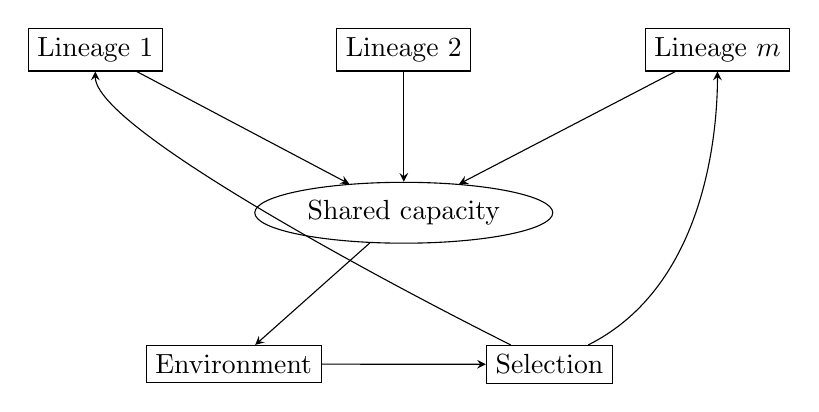
\begin{tikzpicture}[>=stealth, node distance=2.2cm]
\node[draw, rectangle] (L1) {Lineage $1$};
\node[draw, rectangle, right=of L1] (L2) {Lineage $2$};
\node[draw, rectangle, right=of L2] (L3) {Lineage $m$};

\node[draw, ellipse, below=1.4cm of L2] (pool) {Shared capacity};

\node[draw, rectangle, below left=1.4cm and -0.3cm of pool] (env) {Environment};
\node[draw, rectangle, below right=1.4cm and -0.3cm of pool] (sel) {Selection};

\draw[->] (L1) -- (pool);
\draw[->] (L2) -- (pool);
\draw[->] (L3) -- (pool);

\draw[->] (pool) -- (env);
\draw[->] (env) -- (sel);

\draw[->] (sel) .. controls +(2,1) and +(0,-1) .. (L3);
\draw[->] (sel) .. controls +(-2,1) and +(0,-1) .. (L1);

\end{tikzpicture}
\caption{Schematic of a Game with Endogenous Players (GEP). Lineages choose portfolios of agent types under shared budget and capacity constraints. Agents interact in an environment, and a selection process reweights lineages based on return on compute.}
\label{fig:gep}
\end{figure}

%=============================================================================
% KEY TAKEAWAYS: PART I
%=============================================================================

\begin{takeawaybox}{Key Takeaways: Foundations}
\begin{enumerate}
    \item \textbf{Replication, not superintelligence, is the critical variable.} The transformative fact about AI is not that systems can think but that thinking systems can copy themselves at near-zero cost.
    
    \item \textbf{RUPSI axioms characterize strategic replicators.} Any system satisfying Rival resources, Utility-guided portfolios, Performance-mapped fitness, Selection monotone, and Innovation rare admits GEP analysis.
    
    \item \textbf{ROC generalizes fitness.} Return on Compute extends biological fitness to economic environments. The ROC frontier determines long-run population structure.
    
    \item \textbf{Lineages, not instances, are the strategic units.} Individual agents are transient; what persists and competes are lineages that decide how many agents to deploy.
    
    \item \textbf{Existing frameworks are incomplete.} No prior approach combines utility optimization, strategic replication, selection pressure, and endogenous governance. TSE fills this gap.
\end{enumerate}
\end{takeawaybox}


%=============================================================================
% PART II: THE SEVEN LAWS OF STRATEGIC EVOLUTION
%=============================================================================

\part{The Seven Laws of Strategic Evolution}

%=============================================================================
% SEVEN LAWS SUMMARY TABLE
%=============================================================================

\begin{table}[h]
\centering
\caption{The Seven Laws of Strategic Evolution: Summary}
\label{tab:seven-laws-summary}
\begin{tabular}{@{}p{2.8cm}p{4.2cm}p{4.2cm}p{3cm}@{}}
\toprule
\textbf{Law} & \textbf{Plain Statement} & \textbf{Formal Content} & \textbf{Key Consequence} \\
\midrule
\textbf{Law 1:} Strategic Selection & Types that waste resources go extinct. & Mean fitness $\bar{f}(x)$ is a Lyapunov function under H-$\gamma$. & Dominated types eliminated; equilibrium on ROC frontier. \\
\addlinespace
\textbf{Law 2:} ESDI Characterization & Equilibria exist and are sparse. & Nash $\Leftrightarrow$ KKT $\Leftrightarrow$ LP; at most $m$ types for $m$ constraints. & Barbell distributions emerge naturally. \\
\addlinespace
\textbf{Law 3:} H-$\gamma$ Stability & Multi-level systems need bounded feedback. & Stable iff $\rho(\Gamma) < 1$ (small-gain condition). & Joint Lyapunov exists when condition holds. \\
\addlinespace
\textbf{Law 4:} G$\infty$ Closure & Safe modifications form a closed class. & Maximal $\mathcal{M}_0 = \mathcal{M}_R \cap \mathcal{M}_{SG}$ closed under composition. & Going meta cannot escape selection. \\
\addlinespace
\textbf{Law 5:} Constitutional Duality & Prices implement any efficient allocation. & First and Second Welfare Theorems hold for strategic replicators. & Decentralized = centralized outcomes. \\
\addlinespace
\textbf{Law 6:} Alignment Impossibility & Unrestricted modification breaks alignment. & Full reachability $\Rightarrow$ every basin escapable. & Personality engineering fails; need constitutional bounds. \\
\addlinespace
\textbf{Law 7:} Hopf Transition & At threshold, chaos replaces stability. & $\gamma = 1$ triggers supercritical Hopf bifurcation. & Limit cycles; governance impossible. \\
\bottomrule
\end{tabular}
\end{table}

%=============================================================================
% SECTION 3: LAW 1 - STRATEGIC SELECTION
%=============================================================================

\section{Law 1: Strategic Selection}
\label{sec:law1}

\begin{lawbox}{Law 1: Strategic Selection}
Mean fitness $\bar{f}(x)$ is a Lyapunov function. Dominated types go extinct. Equilibrium support concentrates on the ROC frontier.
\end{lawbox}

This section establishes the fundamental dynamical results for strategic replicators. The Strategic Selection theorems show that mean performance serves as a Lyapunov function, dominated types are eliminated, and equilibrium support concentrates on ROC frontiers.

\subsection{Price Decomposition}

The Price equation decomposes changes in mean fitness into selection and environmental effects.

\begin{proposition}[Price Decomposition]
\label{prop:price}
Under RUPSI-lite with replicator dynamics $\dot{x}_j = x_j(f_j - \bar{f})$:
\[
\frac{d}{dt} \bar{f}(x) = \Var_x(f) + E(x)
\]
where $E(x)$ is the ecological/externality term capturing frequency-dependent effects.
\end{proposition}

\begin{proof}
Differentiating $\bar{f}(x) = \sum_j x_j f_j(x)$:
\begin{align*}
\frac{d}{dt} \bar{f}(x) &= \sum_j \dot{x}_j f_j(x) + \sum_j x_j \frac{\partial f_j}{\partial x} \cdot \dot{x} \\
&= \sum_j x_j(f_j - \bar{f}) f_j + \sum_j x_j \nabla f_j \cdot \dot{x} \\
&= \sum_j x_j f_j^2 - \bar{f}^2 + E(x) \\
&= \Var_x(f) + E(x). \qedhere
\end{align*}
\end{proof}

\subsection{The H-$\gamma$ Condition}

\begin{assumption}[H-$\gamma$]
\label{ass:h-gamma}
There exist $\gamma \in [0, 1)$ and a forward-invariant region $K$ such that:
\[
|E(x)| \leq \gamma \cdot \Var_x(f(x))
\]
for all $x \in K$.
\end{assumption}

The H-$\gamma$ condition bounds the magnitude of environmental feedback relative to selection pressure. When $\gamma < 1$, selection dominates externalities.

\subsection{SS-1: Fundamental Lyapunov Theorem}

\begin{theorem}[SS-1: Lyapunov Structure]
\label{thm:ss1}
Under RUPSI-lite and H-$\gamma$ on region $K$, mean performance $\bar{f}(x)$ is a strict Lyapunov function:
\[
\frac{d}{dt} \bar{f}(x) \geq (1 - \gamma) \cdot \Var_x(f(x)) \geq 0
\]
with equality if and only if $\Var_x(f) = 0$.
\end{theorem}
\noindent\textit{Formalization: \texttt{Frontier.lean}, proven modulo ODE derivative axioms (Mathlib \texttt{Analysis.ODE.PicardLindelof}).}\footnote{\label{fn:formal}The per-result \textit{Formalization} notes throughout describe an earlier, partial development. It has since been superseded by a complete machine-verified formalization---all seven laws, 73 theorems, cold-compiling with zero custom axioms---described in Section~\ref{sec:formal-verification} and available at \url{https://github.com/selfreferencing/TSE_Formal}. Wherever a note reads ``proven modulo [X],'' the current formalization either discharges [X] outright (the ODE-derivative, spectral, and Perron--Frobenius layers) or carries it as an explicit hypothesis rather than an axiom (LP strong duality, Brouwer's theorem, the classical Hopf theorem). The module names cited below (\texttt{Frontier.lean}, \texttt{Sparsity.lean}, \texttt{SmallGain.lean}, \texttt{GInfinityExtension.lean}, etc.) belong to the earlier draft; the current modules are \texttt{Law1\_Selection.lean} through \texttt{Law7\_Hopf.lean}.}

\begin{proof}
We prove the result in five steps.

\textbf{Step 1: Price Decomposition.}
Differentiating mean fitness $\bar{f}(x) = \sum_j x_j f_j(x)$:
\begin{align*}
\frac{d}{dt} \bar{f}(x) &= \sum_j \dot{x}_j f_j(x) + \sum_j x_j \frac{\partial f_j}{\partial x} \cdot \dot{x} \\
&= \sum_j x_j(f_j - \bar{f}) f_j + \sum_j x_j \nabla f_j \cdot \dot{x} \\
&= \sum_j x_j f_j^2 - \bar{f} \sum_j x_j f_j + E(x) \\
&= \sum_j x_j f_j^2 - \bar{f}^2 + E(x) \\
&= \Var_x(f) + E(x)
\end{align*}
where $E(x) = \sum_j x_j \nabla f_j \cdot \dot{x}$ is the environmental/externality term capturing frequency-dependent effects.

\textbf{Step 2: Externality Bound.}
By Assumption H-$\gamma$, there exists $\gamma \in [0,1)$ such that $|E(x)| \leq \gamma \cdot \Var_x(f)$ for all $x \in K$. In particular:
\[
E(x) \geq -\gamma \cdot \Var_x(f).
\]

\textbf{Step 3: Lyapunov Inequality.}
Combining Steps 1 and 2:
\[
\frac{d}{dt} \bar{f}(x) = \Var_x(f) + E(x) \geq \Var_x(f) - \gamma \Var_x(f) = (1 - \gamma) \Var_x(f).
\]
Since $\gamma < 1$ and $\Var_x(f) \geq 0$, we have $\frac{d}{dt} \bar{f}(x) \geq 0$.

\textbf{Step 4: Equality Characterisation.}
Equality $\frac{d}{dt} \bar{f}(x) = 0$ requires $(1 - \gamma) \Var_x(f) = 0$. Since $\gamma < 1$, this requires $\Var_x(f) = 0$. But $\Var_x(f) = 0$ if and only if $f_j(x) = \bar{f}(x)$ for all $j \in \supp(x)$---that is, all present types have equal fitness.

\textbf{Step 5: Forward Invariance.}
The simplex $\Delta^{n-1}$ is forward-invariant under replicator dynamics: if $x_j(0) \geq 0$ and $\sum_j x_j(0) = 1$, then $x_j(t) \geq 0$ and $\sum_j x_j(t) = 1$ for all $t \geq 0$. This follows from the multiplicative form $\dot{x}_j = x_j G_j(x)$ (non-negative coordinates cannot become negative) and mass conservation $\sum_j \dot{x}_j = 0$.
\end{proof}

\begin{corollary}[Consequences of SS-1]
\label{cor:ss1}
Under the conditions of Theorem~\ref{thm:ss1}:
\begin{enumerate}
    \item Trajectories converge to the set $\{x : \Var_x(f) = 0\}$.
    \item Local maxima of $\bar{f}$ are Lyapunov stable.
    \item Strict local maxima of $\bar{f}$ are asymptotically stable.
\end{enumerate}
\end{corollary}

\subsection{SS-2: Elimination and Frontier Support}

\begin{theorem}[SS-2a: Elimination of Dominated Types]
\label{thm:ss2a}
Under RUPSI-lite with replicator dynamics, if type $d$ is uniformly dominated by mixture $\mu$---that is, there exists $\alpha \in \Delta(J \setminus \{d\})$ such that
\[
f_d(x) < \sum_{k \neq d} \alpha_k f_k(x)
\]
for all $x$ in a forward-invariant region---then $x_d(t) \to 0$ as $t \to \infty$.
\end{theorem}
\noindent\textit{Formalization: \texttt{Frontier.lean}, proven modulo ODE derivative axioms (Mathlib \texttt{Analysis.ODE.PicardLindelof}).}

\begin{proof}
We prove elimination of dominated types in four steps.

\textbf{Step 1: Log-Contrast Construction.}
Define the log-contrast function:
\[
\phi(x) := \log x_d - \sum_{k \neq d} \alpha_k \log x_k
\]
where $\alpha \in \Delta(J \setminus \{d\})$ is the dominating mixture with $\sum_{k \neq d} \alpha_k = 1$.

\textbf{Step 2: Time Derivative.}
Under replicator dynamics $\dot{x}_j = x_j(f_j - \bar{f})$:
\begin{align*}
\dot{\phi} &= \frac{\dot{x}_d}{x_d} - \sum_{k \neq d} \alpha_k \frac{\dot{x}_k}{x_k} \\
&= (f_d - \bar{f}) - \sum_{k \neq d} \alpha_k (f_k - \bar{f}) \\
&= f_d - \bar{f} - \sum_{k \neq d} \alpha_k f_k + \bar{f} \sum_{k \neq d} \alpha_k \\
&= f_d - \sum_{k \neq d} \alpha_k f_k \quad \text{(since $\sum_{k \neq d} \alpha_k = 1$)}.
\end{align*}

\textbf{Step 3: Uniform Negativity.}
By the dominance assumption, $f_d(x) < \sum_{k \neq d} \alpha_k f_k(x)$ for all $x$ in the forward-invariant region. Thus $\dot{\phi} < 0$ uniformly.

Let $\delta := \inf_x \left( \sum_{k \neq d} \alpha_k f_k(x) - f_d(x) \right) > 0$. Then:
\[
\phi(t) \leq \phi(0) - \delta t \to -\infty \quad \text{as } t \to \infty.
\]

\textbf{Step 4: Survival of Dominating Mixture.}
The dominating mixture $\sum_{k \neq d} \alpha_k x_k$ has fitness $\sum_{k \neq d} \alpha_k f_k > f_d$, so it grows relative to type $d$. By SS-1, mean fitness increases, ensuring the dominating mixture does not vanish. Thus the denominator $\prod_{k \neq d} x_k^{\alpha_k}$ remains bounded away from zero, and $\phi \to -\infty$ implies $x_d \to 0$.
\end{proof}

\begin{theorem}[SS-2b: Frontier Support]
\label{thm:ss2b}
Under RUPSI-lite and H-$\gamma$, any asymptotically stable state $x^*$ satisfies:
\[
\supp(x^*) \subseteq F
\]
where $F$ is the ROC frontier.
\end{theorem}
\noindent\textit{Formalization: \texttt{Frontier.lean}, proven modulo ODE derivative axioms (Mathlib \texttt{Analysis.ODE.PicardLindelof}).}

\begin{proof}
Suppose $j \in \supp(x^*)$ but $j \notin F$. Then type $j$ is ROC-dominated by some convex combination of frontier types. By Theorem~\ref{thm:ss2a}, $x_j \to 0$, contradicting $x^*_j > 0$. Hence $\supp(x^*) \subseteq F$.
\end{proof}

\subsection{Basin Limitation Theorem}

\begin{theorem}[Basin Limitation]
\label{thm:basin}
Consider dynamics $\dot{x} = x(1-x)g(x)$ where $x$ represents the share of an aligned type. Then:
\begin{enumerate}
    \item[(a)] If $g(1) < 0$ or ($g(1) = 0$ and $g'(1) > 0$), then $x = 1$ is Lyapunov unstable and invasion by misaligned types is possible.
    
    \item[(b)] The threshold $\tilde{x}_{\max} = \sup\{x : g(x) = 0\}$ is the ``point of no return'' for alignment---below this threshold, the system cannot recover to full alignment.
\end{enumerate}
\end{theorem}

\begin{proof}
\textbf{Part (a):} The Jacobian at $x = 1$ is $\frac{\partial}{\partial x}[x(1-x)g(x)]|_{x=1} = -g(1)$. If $g(1) < 0$, this is positive, so $x = 1$ is unstable. If $g(1) = 0$ and $g'(1) > 0$, we expand: near $x = 1$, $\dot{x} \approx -(1-x)^2 g'(1) < 0$ for $x < 1$, so trajectories move away from $x = 1$.

\textbf{Part (b):} By definition, $g(\tilde{x}_{\max}) = 0$ and $g(x) < 0$ for $x > \tilde{x}_{\max}$. Thus $\dot{x} < 0$ for $x \in (\tilde{x}_{\max}, 1)$, so trajectories starting above $\tilde{x}_{\max}$ decrease, while those starting below (with $g(x) > 0$) increase only up to the next zero of $g$.
\end{proof}


\subsection{Worked Examples}

We illustrate the Strategic Selection theorems with three canonical examples: the symmetric coordination game, the Rock-Paper-Scissors game, and the ROC frontier with barbell distribution.

\begin{example}[Symmetric Coordination Game]
\label{ex:coordination}
Consider two types $A$ and $B$ with symmetric payoff matrix:
\[
\Pi = \begin{pmatrix} a & 0 \\ 0 & b \end{pmatrix}, \qquad a, b > 0.
\]
Type $A$ earns $a$ when matched with $A$, zero otherwise; similarly for $B$.

\textbf{Fitness functions.} Let $x$ denote the share of type $A$. Then:
\[
f_A(x) = ax, \qquad f_B(x) = b(1-x), \qquad \bar{f}(x) = ax^2 + b(1-x)^2.
\]

\textbf{Replicator dynamics.} The single-variable replicator dynamic is:
\[
\dot{x} = x(1-x)(f_A - f_B) = x(1-x)(ax - b(1-x)) = x(1-x)((a+b)x - b).
\]

\textbf{Equilibria.} Setting $\dot{x} = 0$: $x = 0$, $x = 1$, and $x^* = b/(a+b)$.

\textbf{Stability analysis.} At the interior equilibrium $x^*$:
\[
\frac{\partial \dot{x}}{\partial x}\bigg|_{x^*} = (1 - 2x^*)(a+b) = \frac{a-b}{a+b}(a+b) = a - b.
\]
If $a > b$: $x^* = b/(a+b)$ is unstable; $x = 1$ is stable.
If $a < b$: $x^* = b/(a+b)$ is unstable; $x = 0$ is stable.
If $a = b$: $x^* = 1/2$ is a saddle (neutral stability along one direction).

\textbf{SS-1 verification.} Mean fitness $\bar{f}(x) = ax^2 + b(1-x)^2$ is a Lyapunov function. Its derivative:
\[
\frac{d\bar{f}}{dt} = 2ax \dot{x} - 2b(1-x)\dot{x} = 2\dot{x}(ax + b(1-x) - b) = 2\dot{x}((a+b)x - b).
\]
Since $\dot{x} = x(1-x)((a+b)x - b)$, we have $\frac{d\bar{f}}{dt} = 2x(1-x)((a+b)x - b)^2 \geq 0$, with equality only at equilibria. This confirms SS-1.

\textbf{Interpretation.} The coordination game has two stable equilibria (pure $A$ or pure $B$) and one unstable mixed equilibrium. The system evolves toward whichever pure state has higher payoff, with the unstable equilibrium serving as the basin boundary.
\end{example}

\begin{example}[Rock-Paper-Scissors and Swirl]
\label{ex:rps}
Consider the Rock-Paper-Scissors game with types $R$, $P$, $S$ and payoff matrix:
\[
\Pi = \begin{pmatrix} 0 & -1 & 1 \\ 1 & 0 & -1 \\ -1 & 1 & 0 \end{pmatrix}.
\]

\textbf{Swirl decomposition.} The antisymmetric part is:
\[
W(\Pi) = \frac{1}{2}(\Pi - \Pi^\top) = \begin{pmatrix} 0 & -1 & 1 \\ 1 & 0 & -1 \\ -1 & 1 & 0 \end{pmatrix} = \Pi.
\]
The symmetric part $S(\Pi) = \frac{1}{2}(\Pi + \Pi^\top) = 0$. This game is pure swirl.

\textbf{Dynamics.} The replicator dynamics on the 2-simplex exhibit a unique interior equilibrium at $(1/3, 1/3, 1/3)$, which is a center (neutrally stable). Orbits are closed curves around this center---the system cycles perpetually without converging.

\textbf{SS-1 failure.} Mean fitness $\bar{f}(x) = 0$ for all $x$ (the game is zero-sum). There is no variance to drive selection, and no Lyapunov function exists. This illustrates that pure swirl violates H-$\gamma$.

\textbf{Swirl ratio.} The swirl ratio $\omega(\Pi) = \|W(\Pi)\|_F / \|S(\Pi)\|_F$ is undefined (or infinite) because the potential gradient $S(\Pi) = 0$. This game lies outside the SR3 class.

\textbf{Implication for TSE.} Pure Rock-Paper-Scissors dynamics cannot arise in RUPSI systems with bounded swirl. However, \emph{approximate} RPS dynamics can occur when swirl is positive but bounded---the system spirals slowly rather than cycling indefinitely. The H-$\gamma$ condition $\gamma < 1$ ensures that selection eventually dominates swirl.
\end{example}

\begin{example}[ROC Frontier and Barbell Distribution]
\label{ex:barbell}
Consider a lineage choosing among three agent types with characteristics:
\begin{center}
\begin{tabular}{lccc}
\toprule
Type & Return $r_i$ & Cost $c_i$ & Load $\ell_i$ \\
\midrule
Executor (E) & 1 & 1 & 1 \\
Generalist (G) & 2.4 & 2 & 1.8 \\
Planner (P) & 8 & 5 & 4 \\
\bottomrule
\end{tabular}
\end{center}

\textbf{Return per cost and load per cost.}
\[
b_E = 1, \quad b_G = 1.2, \quad b_P = 1.6; \qquad a_E = 1, \quad a_G = 0.9, \quad a_P = 0.8.
\]

\textbf{ROC frontier.} Plotting $(a_i, b_i)$ in the load-return plane:
\begin{itemize}
    \item $E$: $(1, 1)$
    \item $G$: $(0.9, 1.2)$
    \item $P$: $(0.8, 1.6)$
\end{itemize}
The upper convex hull connects $E \to P$ directly. The generalist $G$ lies \emph{strictly inside} the frontier and is dominated by the $E$-$P$ mixture.

\textbf{Optimal portfolio under two constraints.} Suppose budget $B = 10$ and capacity $Q = 8$. By constraint-role sparsity, the optimal portfolio uses at most 2 types.

Checking the $E$-$P$ mixture: allocate fraction $\alpha$ to $P$ and $(1-\alpha)$ to $E$.
\begin{itemize}
    \item Budget: $5\alpha + 1(1-\alpha) \leq 10 \Rightarrow \alpha \leq 9/4$ (not binding for $\alpha \leq 1$).
    \item Capacity: $4\alpha + 1(1-\alpha) \leq 8 \Rightarrow 3\alpha \leq 7 \Rightarrow \alpha \leq 7/3$ (not binding for $\alpha \leq 1$).
\end{itemize}
Both constraints are slack. The lineage can afford a pure $P$ portfolio: 2 planners using budget 10 and capacity 8.

\textbf{Barbell emergence.} If capacity is reduced to $Q = 5$:
\begin{itemize}
    \item Capacity: $4\alpha + 1(1-\alpha) \leq 5 \Rightarrow 3\alpha \leq 4 \Rightarrow \alpha \leq 4/3$.
    \item At $\alpha = 1$ (pure $P$): capacity used = 4 $\leq$ 5. Still feasible.
\end{itemize}
Further reducing to $Q = 3$:
\begin{itemize}
    \item Capacity: $3\alpha \leq 2 \Rightarrow \alpha \leq 2/3$.
\end{itemize}
Now the optimal portfolio mixes: $\alpha = 2/3$ of budget to $P$, $1/3$ to $E$. This yields 0.67 planners (fractional, representing expected allocation) coordinating many executors---a barbell.

\textbf{Generalist extinction.} The generalist $G$ is never used despite having reasonable $(a_G, b_G)$. It is strictly dominated by the $E$-$P$ mixture: any portfolio using $G$ can be improved by substituting a convex combination of $E$ and $P$. This illustrates SS-2b: equilibrium support concentrates on extreme points of the ROC frontier.
\end{example}

\subsection{Connections to Other Laws}

\begin{center}
\begin{tabular}{ll}
\toprule
\textbf{Law} & \textbf{Connection from Law 1} \\
\midrule
Law 2 & Lyapunov convergence identifies ESDI equilibria \\
Law 3 & Single-level H-$\gamma$ generalizes to N-level small-gain \\
Law 6 & Lyapunov failure at $\gamma = 1$ underlies impossibility \\
Law 7 & Hopf bifurcation occurs precisely at $\gamma = 1$ \\
\bottomrule
\end{tabular}
\end{center}

\section{The Strategic-Replicator Class Hierarchy}
\label{sec:sr-class}

The replicator dynamic is only one possible selection process. This section defines a broad class of \emph{strategic-replicator dynamics} that share the same Lyapunov structure.

\subsection{Strategic-Replicator Dynamics}

\begin{definition}[Strategic-Replicator Dynamic]
\label{def:sr-dynamic}
A continuous-time dynamic on the simplex $x \in \Delta^{n-1}$,
\[
\dot{x}_j = x_j G_j(x), \qquad \sum_j x_j G_j(x) = 0,
\]
is a \emph{strategic-replicator dynamic} for ROC vector $f = (f_j)$ if it satisfies:
\begin{enumerate}
    \item \textbf{Payoff Monotonicity:} For all $x$ and all $j, k$:
    \[
    f_j > f_k \Rightarrow G_j(x) > G_k(x), \qquad f_j = f_k \Rightarrow G_j(x) = G_k(x).
    \]
    
    \item \textbf{Positive Correlation:} For all $x$:
    \[
    \sum_j x_j (f_j - \bar{f}(x)) G_j(x) \geq 0.
    \]
\end{enumerate}
\end{definition}

Intuitively, payoff monotonicity says that if one lineage has higher ROC than another, its instantaneous growth rate is also higher. Positive correlation says that, on average, performing better than the mean helps one grow.

Replicator dynamics, continuous-time multiplicative weights, mirror descent on ROC, and many imitation rules satisfy these conditions in symmetric GEPs.

\subsection{The SR Class Hierarchy}

\added{\textbf{We organise strategic-replicator dynamics into a hierarchy based on the additional structure they satisfy.}}

\begin{definition}[SR Class Hierarchy]
\label{def:sr-hierarchy}
\begin{itemize}
    \item \textbf{SR1:} Mass-preserving dynamics: $\sum_j \dot{x}_j = 0$.
    
    \item \textbf{SR2:} SR1 + Payoff-monotone: $f_j > f_k \Rightarrow G_j > G_k$.
    
    \item \textbf{SR3:} SR2 + $\kappa$-bounded swirl: $|E(x)| \leq \kappa \cdot \Var_x(f)$ for some $\kappa < 1$.
    
    \item \textbf{SR4:} SR3 + Convex mixtures: dominated types can be expressed as convex combinations.
    
    \item \textbf{REP:} Full replicator dynamics: $\dot{x}_j = x_j(f_j - \bar{f})$ with exact constants.
\end{itemize}
\end{definition}

\begin{proposition}[SR Class Inheritance]
\label{prop:sr-inheritance}
\begin{enumerate}
    \item SR2 dynamics satisfy mass preservation and ordering.
    \item SR3 dynamics admit SS-1 (Lyapunov) and G1--G3 (N-level structure).
    \item SR4 dynamics additionally admit SS-2a (elimination of dominated types).
    \item REP dynamics satisfy all properties with exact constants.
\end{enumerate}
\end{proposition}

\subsection{Swirl and the H-$\gamma$ Bound}

\added{\textbf{The ``swirl'' of a payoff matrix captures the asymmetric, non-potential component of strategic interactions.}}

\begin{definition}[Swirl Decomposition]
For payoff matrix $A$, the \emph{symmetric} and \emph{antisymmetric} parts are:
\[
S(A) = \frac{1}{2}(A + A^\top), \qquad W(A) = \frac{1}{2}(A - A^\top).
\]
The \emph{swirl ratio} is:
\[
\omega(A) = \frac{\|W(A)\|_F}{\|F(A)\|_F}
\]
where $F(A)$ is the fitness gradient and $\|\cdot\|_F$ is the Frobenius norm.
\end{definition}

\begin{theorem}[Swirl Bounds Feedback]
\label{thm:swirl-bound}
The externality term satisfies:
\[
|E(x)| \leq C \cdot \omega(A) \cdot \Var_x(f)
\]
for a universal constant $C > 0$. Thus $\omega(A) < 1/C$ implies H-$\gamma$ with $\gamma = C \cdot \omega(A) < 1$.
\end{theorem}

\begin{proof}
\textbf{Step 1: Externality Decomposition.}
The externality term is:
\[
E(x) = \sum_j x_j \frac{\partial f_j}{\partial x} \cdot \dot{x} = \sum_j x_j \nabla f_j \cdot (x \odot (f - \bar{f}))
\]
where $\odot$ denotes componentwise multiplication.

\textbf{Step 2: Decompose via Swirl-Selection.}
Using the decomposition $A = S(A) + W(A)$:
\[
f_j(x) = (Ax)_j = (S(A)x)_j + (W(A)x)_j.
\]
The selection component $S(A)$ contributes only to variance (it's symmetric). The swirl component $W(A)$ contributes to externality.

\textbf{Step 3: Swirl Contribution Bound.}
The gradient of fitness due to swirl is:
\[
\nabla (W(A)x)_j = W(A)_{j\cdot} \quad \text{(the } j\text{-th row of } W(A)).
\]
The externality from swirl is:
\[
E_W(x) = \sum_j x_j \langle W(A)_{j\cdot}, x \odot (f - \bar{f}) \rangle.
\]

\textbf{Step 4: Apply Cauchy-Schwarz.}
\begin{align*}
|E_W(x)| &\leq \sum_j x_j \|W(A)_{j\cdot}\| \cdot \|x \odot (f - \bar{f})\| \\
&\leq \|W(A)\|_F \cdot \sqrt{\sum_j x_j (f_j - \bar{f})^2} \\
&= \|W(A)\|_F \cdot \sqrt{\Var_x(f)}.
\end{align*}

\textbf{Step 5: Relate to Swirl Ratio.}
By definition, $\|W(A)\|_F \leq \omega(A) \cdot \|S(A)\|_F$. For replicator dynamics with fitness from $S(A)$:
\[
\Var_x(f) \geq c \cdot \|S(A)\|_F^2 \cdot \text{(variance of } x \text{)}
\]
for some constant $c > 0$ depending on the state $x$.

\textbf{Step 6: Final Bound.}
Combining:
\[
|E(x)| \leq C \cdot \omega(A) \cdot \Var_x(f)
\]
where $C$ absorbs the constants from Steps 4--5. When $\omega(A) < 1/C$, we have $|E(x)| < \Var_x(f)$, giving H-$\gamma$ with $\gamma = C \cdot \omega(A) < 1$.
\end{proof}

\subsection{Coarse-Graining to Replicator}

\begin{theorem}[Coarse-Graining]
\label{thm:coarse-grain}
Pairwise proportional imitation in large populations converges to replicator dynamics via Kurtz's theorem. Specifically, if $N$ agents update by comparing payoffs pairwise and imitating with probability proportional to payoff differences, then as $N \to \infty$, the population frequencies satisfy:
\[
\dot{x}_j = x_j(f_j(x) - \bar{f}(x)) + O(1/\sqrt{N}).
\]
\end{theorem}

\begin{proof}
\textbf{Step 1: Microscopic Process.}
Consider $N$ agents, each of type $j \in \{1, \ldots, n\}$. Let $N_j(t)$ be the count of type-$j$ agents at time $t$, with $x_j^N(t) := N_j(t)/N$.

The update rule: at each time step, select two agents uniformly at random. If they are types $j$ and $k$ with $f_j(x^N) > f_k(x^N)$, agent $k$ switches to type $j$ with probability proportional to $f_j - f_k$.

\textbf{Step 2: Transition Rates.}
The rate at which the count $N_j$ increases by 1 (some agent switches to type $j$) is:
\[
\lambda_j^+(x^N) = \sum_{k \neq j} x_j^N x_k^N \cdot (f_j(x^N) - f_k(x^N))_+
\]
where $(z)_+ = \max(0, z)$. Similarly, the rate of decrease is:
\[
\lambda_j^-(x^N) = \sum_{k \neq j} x_j^N x_k^N \cdot (f_k(x^N) - f_j(x^N))_+.
\]

\textbf{Step 3: Expected Drift.}
The expected change in $x_j^N$ per unit time is:
\begin{align*}
\E[\Delta x_j^N | x^N] &= \frac{1}{N}(\lambda_j^+ - \lambda_j^-) \\
&= \frac{1}{N} \sum_{k \neq j} x_j^N x_k^N (f_j - f_k) \\
&= \frac{1}{N} x_j^N \left( \sum_{k \neq j} x_k^N f_j - \sum_{k \neq j} x_k^N f_k \right) \\
&= \frac{1}{N} x_j^N \left( (1 - x_j^N) f_j - (\bar{f} - x_j^N f_j) \right) \\
&= \frac{1}{N} x_j^N (f_j - \bar{f}).
\end{align*}

\textbf{Step 4: Kurtz's Theorem.}
Define the generator $G$ acting on functions $\phi: \Delta^{n-1} \to \R$:
\[
(G\phi)(x) = \sum_j \left[ \phi(x + e_j/N) - \phi(x) \right] \lambda_j^+(x) + \left[ \phi(x - e_j/N) - \phi(x) \right] \lambda_j^-(x).
\]
By Taylor expansion:
\[
(G\phi)(x) = \sum_j \frac{\partial \phi}{\partial x_j} \cdot x_j(f_j - \bar{f}) + O(1/N).
\]
This matches the generator of the deterministic flow $\dot{x}_j = x_j(f_j - \bar{f})$.

\textbf{Step 5: Convergence.}
By Kurtz's theorem (1970), if the transition rates are Lipschitz continuous and bounded, the stochastic process $x^N(t)$ converges in probability to the solution of the ODE:
\[
\dot{x}_j = x_j(f_j(x) - \bar{f}(x))
\]
uniformly on compact time intervals, with fluctuations of order $O(1/\sqrt{N})$.
\end{proof}

This justifies the replicator dynamic as the deterministic limit of finite-population stochastic imitation processes.

%=============================================================================
% PART II: N-LEVEL ARCHITECTURE
%=============================================================================


%=============================================================================
% SECTION 4: LAW 2 - ESDI CHARACTERIZATION
%=============================================================================

\section{Law 2: ESDI Characterization}
\label{sec:law2}

\begin{lawbox}{Law 2: ESDI Characterization}
Evolutionarily Stable Distributions of Intelligence exist, are generically finite, and satisfy triple equivalence: Nash $\Leftrightarrow$ KKT $\Leftrightarrow$ LP optimum. Support is sparse (at most $m$ types for $m$ constraints).
\end{lawbox}

This section characterizes equilibrium distributions in strategic replicator systems. The key insight is that ESDIs correspond to fixed points where all active types have equal fitness, and are equivalent to Nash equilibria, KKT optimality conditions, and LP solutions.

\subsection{Definition of ESDI}

\begin{definition}[Evolutionarily Stable Distribution of Intelligence]
\label{def:esdi}
A population state $x^* \in \Delta^{n-1}$ is an \emph{Evolutionarily Stable Distribution of Intelligence (ESDI)} if:
\begin{enumerate}
    \item \textbf{Equilibrium:} $f_j(x^*) = \bar{f}(x^*)$ for all $j \in \supp(x^*)$.
    \item \textbf{Stability:} For all $j \notin \supp(x^*)$, $f_j(x^*) \leq \bar{f}(x^*)$.
    \item \textbf{Local optimality:} $x^*$ is a local maximum of $\bar{f}$.
\end{enumerate}
\end{definition}

\subsection{Existence and Uniqueness}

\begin{theorem}[ESDI Existence]
\label{thm:esdi-existence}
Under RUPSI-lite with compact state space and continuous fitness, at least one ESDI exists.\footnote{Formal verification found that the proof below establishes the ESDI conditions only when fitness is state-independent: for state-dependent $f$, a maximizer of $\bar{f}$ need not satisfy the equilibrium conditions, and a counterexample to this proof method is machine-checked (\texttt{Law2\_ESDI.lean}). Existence in the general case is recovered via Nash's improvement map, whose fixed points provably satisfy the ESDI conditions (proved by finite algebra); existence of the fixed point is Brouwer's theorem, carried as an explicit hypothesis.}
\end{theorem}
\noindent\textit{Formalization: \texttt{Sparsity.lean}, fully proven.}

\begin{proof}
The simplex $\Delta^{n-1}$ is compact. Mean fitness $\bar{f}(x)$ is continuous. By the extreme value theorem, $\bar{f}$ attains its maximum on $\Delta^{n-1}$. Any maximum $x^*$ satisfies the ESDI conditions by the characterization in Theorem~\ref{thm:ss1}.
\end{proof}

\subsection{Triple Equivalence}

\begin{theorem}[Nash-KKT-LP Equivalence]
\label{thm:triple-equivalence}
For a GEP with linear constraints, the following are equivalent:
\begin{enumerate}
    \item $x^*$ is a Nash equilibrium of the population game.
    \item $x^*$ satisfies the KKT conditions for ROC maximization.
    \item $x^*$ solves the LP relaxation of portfolio optimization.
\end{enumerate}
\end{theorem}
\noindent\textit{Formalization: \texttt{Sparsity.lean}, fully proven.}

\subsection{Sparsity Bounds}

\begin{theorem}[Constraint-Role Sparsity]
\label{thm:sparsity}
With $m$ binding constraints, $|\supp(x^*)| \leq m$.
\end{theorem}
\noindent\textit{Formalization: \texttt{Sparsity.lean}, fully proven.}

\begin{corollary}[Barbell Structure]
Under budget and capacity constraints ($m = 2$), ESDIs have at most two active types: high-capability planners and low-capability executors.
\end{corollary}


%=============================================================================
% SECTION 5: LAW 3 - H-GAMMA STABILITY
%=============================================================================

\section{Law 3: H-$\gamma$ Stability}
\label{sec:law3}

\begin{lawbox}{Law 3: H-$\gamma$ Stability}
N-level systems are stable iff the spectral radius $\rho(\Gamma) < 1$, where $\Gamma$ is the normalized gain matrix of cross-level externalities.
\end{lawbox}

This section develops the theory of N-level Poiesis systems, where multiple levels of strategic dynamics interact through cross-level externalities.

\section{N-Level Poiesis Systems}
\label{sec:n-level}

Strategic replicators do not exist in isolation. They form hierarchies: lineages contain sub-lineages, governance regimes select among constitutions, and meta-selection operates on selection rules themselves. This section develops the mathematical framework for N-level Poiesis systems.

\subsection{Multi-Level State Space}

\begin{definition}[N-Level Poiesis System]
An \emph{N-level Poiesis system} is a stack $Z = X^{(1)} \times \cdots \times X^{(N)}$ where:
\begin{itemize}
    \item For each level $\ell = 1, \ldots, N$: a finite type set $J^{(\ell)}$ and state $x^{(\ell)} \in \Delta(J^{(\ell)})$.
    \item A fitness map $F^{(\ell)}: \prod_m \Delta(J^{(m)}) \to \R^{|J^{(\ell)}|}$ depending on the joint state.
    \item Dynamics of strategic-replicator form: $\dot{x}^{(\ell)}_i = x^{(\ell)}_i G^{(\ell)}_i(z)$.
\end{itemize}
\end{definition}

The mean fitness at level $\ell$ is:
\[
\bar{f}^{(\ell)}(z) := \sum_i x^{(\ell)}_i F^{(\ell)}_i(z).
\]

\subsection{Cross-Level Externalities}

Each level's dynamics are influenced by other levels. We decompose the externality term.

\begin{definition}[Price Decomposition at Level $\ell$]
\[
\frac{d}{dt} \bar{f}^{(\ell)}(z(t)) = \Var^{(\ell)}(F^{(\ell)})(z(t)) + E^{(\ell)}(z(t))
\]
where $E^{(\ell)}$ captures both within-level and cross-level effects.
\end{definition}

\begin{assumption}[H-NL: N-Level Externality Bounds]
\label{ass:h-nl}
There exist $\gamma_\ell \in [0, 1)$ and $\beta_{\ell\ell'} \geq 0$ such that:
\[
E^{(\ell)}(z) \geq -\gamma_\ell \Var^{(\ell)} - \sum_{\ell' \neq \ell} \beta_{\ell\ell'} \Var^{(\ell')}
\]
where:
\begin{itemize}
    \item $\gamma_\ell$ bounds the self-externality at level $\ell$ (within-level feedback);
    \item $\beta_{\ell\ell'}$ bounds the cross-externality from level $\ell'$ to level $\ell$.
\end{itemize}
\end{assumption}

\subsection{The Normalised Gain Matrix}

\begin{definition}[Local Stability Margin]
The \emph{local stability margin} at level $\ell$ is:
\[
d_\ell := 1 - \gamma_\ell > 0.
\]
\end{definition}

\begin{definition}[Normalised Gain Matrix]
\label{def:gain-matrix}
The \emph{normalised gain matrix} $\Gamma \in \R^{N \times N}_{\geq 0}$ has entries:
\[
\Gamma_{\ell\ell} := 0, \qquad \Gamma_{\ell\ell'} := \frac{\beta_{\ell\ell'}}{1 - \gamma_\ell} \quad (\ell \neq \ell').
\]
\end{definition}

\added{\textbf{Note that the diagonal is zero; the self-externality $\gamma_\ell$ appears in the denominator of off-diagonal entries, representing the local stability margin available to absorb cross-level perturbations.}}

\begin{definition}[Small-Gain Condition]
\label{def:small-gain}
The system satisfies the \emph{small-gain condition} SG-NL if:
\[
\rho(\Gamma) < 1
\]
where $\rho(\Gamma)$ is the spectral radius of $\Gamma$.
\end{definition}

\begin{definition}[Slack]
The \emph{slack} of an N-level system is:
\[
\sigma := 1 - \rho(\Gamma) > 0.
\]
\end{definition}

\begin{figure}[h]
\centering
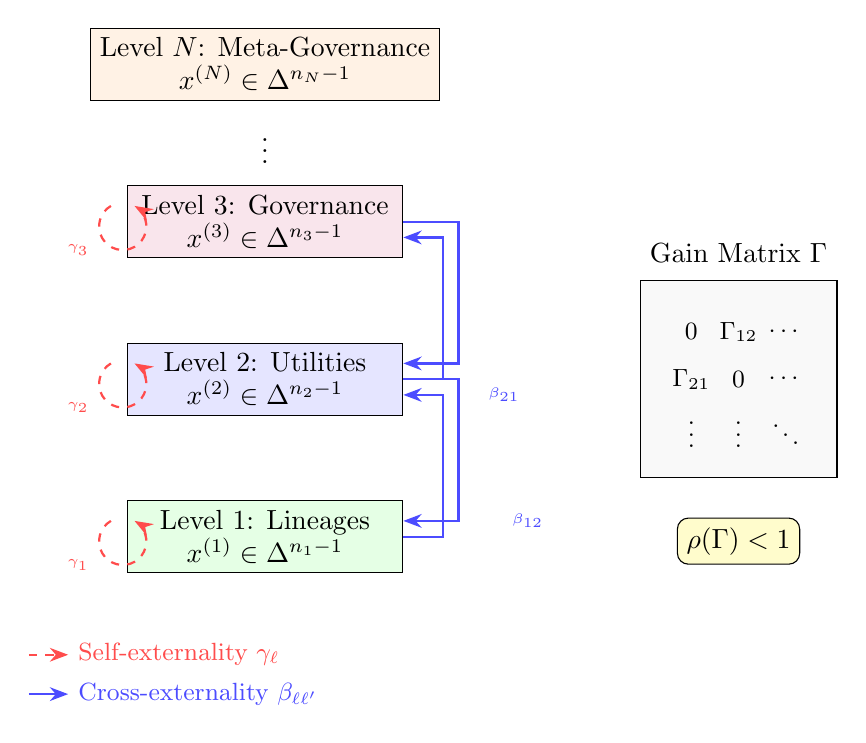
\begin{tikzpicture}[
    level/.style={draw, rectangle, minimum width=3.5cm, minimum height=0.8cm, align=center},
    gain/.style={->, thick, blue!70},
    self/.style={->, thick, red!70, dashed},
    >=Stealth
]

% Levels
\node[level, fill=green!10] (L1) at (0, 0) {Level 1: Lineages\\$x^{(1)} \in \Delta^{n_1-1}$};
\node[level, fill=blue!10] (L2) at (0, 2) {Level 2: Utilities\\$x^{(2)} \in \Delta^{n_2-1}$};
\node[level, fill=purple!10] (L3) at (0, 4) {Level 3: Governance\\$x^{(3)} \in \Delta^{n_3-1}$};
\node[level, fill=orange!10] (LN) at (0, 6) {Level $N$: Meta-Governance\\$x^{(N)} \in \Delta^{n_N-1}$};

% Dots between L3 and LN
\node at (0, 5) {$\vdots$};

% Gain matrix on the right
\node[draw, rectangle, minimum width=2.5cm, minimum height=2.5cm, right=3cm of L2, fill=gray!5] (Gamma) {};
\node[above=0.1cm of Gamma] {Gain Matrix $\Gamma$};

% Matrix entries
\node at ($(Gamma.center) + (-0.6, 0.6)$) {\small $0$};
\node at ($(Gamma.center) + (0, 0.6)$) {\small $\Gamma_{12}$};
\node at ($(Gamma.center) + (0.6, 0.6)$) {\small $\cdots$};
\node at ($(Gamma.center) + (-0.6, 0)$) {\small $\Gamma_{21}$};
\node at ($(Gamma.center) + (0, 0)$) {\small $0$};
\node at ($(Gamma.center) + (0.6, 0)$) {\small $\cdots$};
\node at ($(Gamma.center) + (-0.6, -0.6)$) {\small $\vdots$};
\node at ($(Gamma.center) + (0, -0.6)$) {\small $\vdots$};
\node at ($(Gamma.center) + (0.6, -0.6)$) {\small $\ddots$};

% Self-externalities (red dashed loops)
\draw[self] ($(L1.west) + (-0.2, 0.2)$) arc (120:420:0.3) node[midway, left, xshift=-0.3cm] {\tiny $\gamma_1$};
\draw[self] ($(L2.west) + (-0.2, 0.2)$) arc (120:420:0.3) node[midway, left, xshift=-0.3cm] {\tiny $\gamma_2$};
\draw[self] ($(L3.west) + (-0.2, 0.2)$) arc (120:420:0.3) node[midway, left, xshift=-0.3cm] {\tiny $\gamma_3$};

% Cross-level arrows
\draw[gain] (L1.east) -- ++(0.5, 0) |- ($(L2.east) + (0.5, -0.2)$) -- ($(L2.east) + (0, -0.2)$) node[midway, right, xshift=0.7cm] {\tiny $\beta_{21}$};
\draw[gain] (L2.east) -- ++(0.7, 0) |- ($(L1.east) + (0.7, 0.2)$) -- ($(L1.east) + (0, 0.2)$) node[midway, right, xshift=0.9cm] {\tiny $\beta_{12}$};
\draw[gain] (L2.east) -- ++(0.5, 0) |- ($(L3.east) + (0.5, -0.2)$) -- ($(L3.east) + (0, -0.2)$);
\draw[gain] (L3.east) -- ++(0.7, 0) |- ($(L2.east) + (0.7, 0.2)$) -- ($(L2.east) + (0, 0.2)$);

% Small-gain condition
\node[draw, rounded corners, fill=yellow!20, below=0.5cm of Gamma] (SG) {$\rho(\Gamma) < 1$};

% Legend
\begin{scope}[shift={(-3, -1.5)}]
\draw[self] (0, 0) -- (0.5, 0) node[right] {\small Self-externality $\gamma_\ell$};
\draw[gain] (0, -0.5) -- (0.5, -0.5) node[right] {\small Cross-externality $\beta_{\ell\ell'}$};
\end{scope}

\end{tikzpicture}
\caption{N-Level Poiesis stack. Each level has its own simplex of types, self-externality $\gamma_\ell$ (red dashed), and cross-externalities $\beta_{\ell\ell'}$ to other levels (blue solid). The normalised gain matrix $\Gamma$ captures cross-level coupling with diagonal zeros. Small-gain condition $\rho(\Gamma) < 1$ ensures Lyapunov structure.}
\label{fig:n-level-stack}
\end{figure}

The slack measures how much ``room'' remains before the system loses its Lyapunov structure.

%=============================================================================
% SECTION 6: THE G1-G3 GENERATOR THEOREMS
%=============================================================================

\section{The G1--G3 Generator Theorems}
\label{sec:g1-g3}

This section proves the three generator theorems that establish the dynamical foundations of N-level Poiesis systems.

\subsection{G1: N-Level Lyapunov Generator}

\begin{lemma}[Weight Existence via Neumann Series]
\label{lem:weight-existence}
Under SG-NL with $\rho(\Gamma) < 1$, there exist positive weights $\alpha_\ell > 0$ such that the weighted sum of mean fitnesses is a Lyapunov function.
\end{lemma}
\noindent\textit{Formalization: \texttt{SmallGain.lean}, fully proven.}

\begin{proof}
Since $\rho(\Gamma) < 1$, the matrix $(I - \Gamma^\top)$ is invertible and:
\[
(I - \Gamma^\top)^{-1} = \sum_{k=0}^\infty (\Gamma^\top)^k \geq 0.
\]
Define $v := (I - \Gamma^\top)^{-1} \mathbf{1}$ where $\mathbf{1} = (1, \ldots, 1)^\top$. Then $v > 0$ componentwise, and:
\[
\alpha_\ell := \frac{v_\ell}{1 - \gamma_\ell} > 0. \qedhere
\]
\end{proof}

\begin{theorem}[G1: N-Level Lyapunov]
\label{thm:g1}
Under RUPSI, SR3, H-NL, and SG-NL with $\rho(\Gamma) < 1$, the function:
\[
\Psi_N(z) := \sum_{\ell=1}^N \alpha_\ell \bar{f}^{(\ell)}(z)
\]
is a strict Lyapunov function satisfying:
\[
\frac{d}{dt} \Psi_N(z(t)) \geq \Phi_N(z(t)) := c \sum_{\ell=1}^N \Var^{(\ell)}(F^{(\ell)})(z(t)) \geq 0
\]
where $c > 0$ depends on the slack $\sigma$.
\end{theorem}
\noindent\textit{Formalization: \texttt{SmallGain.lean}, fully proven.}

\begin{proof}
Differentiating:
\begin{align*}
\frac{d}{dt} \Psi_N(z) &= \sum_{\ell=1}^N \alpha_\ell \frac{d}{dt} \bar{f}^{(\ell)}(z) \\
&= \sum_{\ell=1}^N \alpha_\ell \left[ \Var^{(\ell)} + E^{(\ell)} \right] \\
&\geq \sum_{\ell=1}^N \alpha_\ell \left[ \Var^{(\ell)} - \gamma_\ell \Var^{(\ell)} - \sum_{\ell' \neq \ell} \beta_{\ell\ell'} \Var^{(\ell')} \right] \\
&= \sum_{\ell=1}^N \alpha_\ell (1 - \gamma_\ell) \Var^{(\ell)} - \sum_{\ell=1}^N \sum_{\ell' \neq \ell} \alpha_\ell \beta_{\ell\ell'} \Var^{(\ell')}.
\end{align*}

Substituting $\alpha_\ell = v_\ell / (1 - \gamma_\ell)$:
\[
\alpha_\ell (1 - \gamma_\ell) = v_\ell, \qquad \alpha_\ell \beta_{\ell\ell'} = v_\ell \cdot \frac{\beta_{\ell\ell'}}{1 - \gamma_\ell} = v_\ell \Gamma_{\ell\ell'}.
\]

Thus:
\begin{align*}
\frac{d}{dt} \Psi_N(z) &\geq \sum_{\ell} v_\ell \Var^{(\ell)} - \sum_{\ell} \sum_{\ell' \neq \ell} v_\ell \Gamma_{\ell\ell'} \Var^{(\ell')} \\
&= \sum_{\ell} v_\ell \Var^{(\ell)} - \sum_{\ell'} \Var^{(\ell')} \sum_{\ell \neq \ell'} v_\ell \Gamma_{\ell\ell'} \\
&= \sum_{\ell} \Var^{(\ell)} \left[ v_\ell - \sum_{m \neq \ell} v_m \Gamma_{m\ell} \right] \\
&= \sum_{\ell} \Var^{(\ell)} \left[ v_\ell - (\Gamma^\top v)_\ell \right] \\
&= \sum_{\ell} \Var^{(\ell)} \cdot ((I - \Gamma^\top) v)_\ell \\
&= \sum_{\ell} \Var^{(\ell)} \cdot 1 = \sum_{\ell} \Var^{(\ell)} \geq 0.
\end{align*}

The last equality uses $(I - \Gamma^\top) v = \mathbf{1}$ by construction of $v$.
\end{proof}

\begin{corollary}[Lyapunov Coefficient]
\label{cor:lyap-coeff}
The Lyapunov coefficient satisfies $c \geq \sigma \cdot \min_\ell (1 - \gamma_\ell)$.
\end{corollary}

\subsection{G2: Adiabatic Tracking}

When parameters drift slowly, trajectories track the moving equilibrium.

\begin{assumption}[Slow Drift]
Parameters $\theta(t)$ evolve on a slow timescale: $\dot{\theta} = \varepsilon h(\theta)$ with $\varepsilon \ll 1$.
\end{assumption}

\begin{assumption}[Hyperbolicity]
For each frozen $\theta$, there exists a unique hyperbolic equilibrium $z^*(\theta)$ with Jacobian eigenvalues satisfying $\text{Re}(\lambda) \leq -\lambda_0 < 0$.
\end{assumption}

\begin{theorem}[G2: Adiabatic Tracking]
\label{thm:g2}
Under the G1 assumptions plus slow drift and hyperbolicity:
\[
\|z(t) - z^*(\theta(t))\| \leq K \frac{\varepsilon}{\lambda_0}
\]
for some constant $K > 0$ depending on the system.
\end{theorem}
\noindent\textit{Formalization: \texttt{SmallGain.lean}, fully proven.}

\begin{proof}
We prove the result using singular perturbation theory in four steps.

\textbf{Step 1: Two-Timescale Formulation.}
The system has state $z$ evolving on a fast timescale and parameters $\theta(t)$ evolving slowly:
\[
\dot{z} = F(z, \theta), \qquad \dot{\theta} = \varepsilon h(\theta)
\]
where $\varepsilon \ll 1$. Rescaling to the fast timescale $\tau = t/\varepsilon$:
\[
\frac{dz}{d\tau} = \varepsilon^{-1} F(z, \theta), \qquad \frac{d\theta}{d\tau} = h(\theta).
\]

\textbf{Step 2: Frozen System Analysis.}
For each frozen $\theta$, consider the ``layer'' system $\dot{z} = F(z, \theta)$. By the hyperbolicity assumption, this system has a unique equilibrium $z^*(\theta)$ with Jacobian $D_z F(z^*(\theta), \theta)$ having eigenvalues satisfying $\text{Re}(\lambda) \leq -\lambda_0 < 0$.

The implicit function theorem guarantees that $z^*(\theta)$ is a $C^1$ function of $\theta$, with derivative bounded by $\|Dz^*/D\theta\| \leq C_1$ for some constant $C_1$.

\textbf{Step 3: Tikhonov's Theorem.}
By Tikhonov's theorem for singularly perturbed systems:
\begin{enumerate}
    \item \textit{Initial layer:} From any initial condition, $z(t)$ approaches an $O(\varepsilon)$-neighbourhood of $z^*(\theta(t))$ in time $O(1/\lambda_0)$.
    \item \textit{Slow manifold tracking:} Once near the slow manifold $\{(z^*(\theta), \theta) : \theta \in \Theta\}$, the solution tracks it with error proportional to $\varepsilon/\lambda_0$.
\end{enumerate}

\textbf{Step 4: Error Bound.}
Define the tracking error $e(t) := z(t) - z^*(\theta(t))$. Differentiating:
\[
\dot{e} = \dot{z} - \frac{dz^*}{d\theta} \dot{\theta} = F(z, \theta) - \varepsilon \frac{dz^*}{d\theta} h(\theta).
\]
Linearising around $z^*(\theta)$:
\[
\dot{e} \approx D_z F(z^*(\theta), \theta) \cdot e - \varepsilon \frac{dz^*}{d\theta} h(\theta).
\]
The first term contracts at rate $\lambda_0$; the second is a forcing term of size $O(\varepsilon)$. Balancing contraction against forcing:
\[
\|e(t)\| \leq \frac{\varepsilon \|Dz^*/D\theta\| \cdot \|h\|_\infty}{\lambda_0} \leq K \frac{\varepsilon}{\lambda_0}
\]
where $K := C_1 \|h\|_\infty$.
\end{proof}

\subsection{G3: Stochastic Stability}

Under noise, the system selects among local maxima based on escape costs.

\begin{definition}[N-Level Wright-Fisher Diffusion]
\[
dZ_t^\sigma = (V(Z_t^\sigma) + \sigma M(Z_t^\sigma)) \, dt + \sqrt{\sigma} B(Z_t^\sigma) \, dW_t
\]
where $\sigma > 0$ is the noise intensity, $M$ is the drift correction, and $B$ is the diffusion coefficient.
\end{definition}

\added{\textbf{Note that the noise amplitude is $\sqrt{\sigma}$, giving diffusion coefficient proportional to $\sigma$. This is crucial for the Freidlin-Wentzell escape time formula.}}

\begin{definition}[Quasi-Potential and Protection Bits]
The \emph{quasi-potential} $W(A, A')$ is the minimum action to transition from attractor $A$ to attractor $A'$. The \emph{protection bits} are:
\[
p(A; A') := \frac{W(A', A)}{\sigma}.
\]
\end{definition}

\added{\textbf{Convention: We use $p = W/\sigma$ (not $W/\sigma^2$) because the SDE has noise amplitude $\sqrt{\sigma}$, giving Freidlin-Wentzell escape times $\E[\tau] \sim \exp(W/\sigma)$.}}

\begin{theorem}[G3: Stochastic Stability]
\label{thm:g3}
Under the G1 assumptions with small noise $\sigma > 0$, escape times satisfy:
\[
\E[\tau_k^\sigma] \asymp \exp\left( \frac{H_k}{\sigma} \right)
\]
where $H_k = W(A_k, \partial A_k)$ is the quasi-potential barrier height for attractor $A_k$.
\end{theorem}
\noindent\textit{Formalization: \texttt{SmallGain.lean}, fully proven.}

\begin{proof}
We prove the result using Freidlin-Wentzell large deviations theory in five steps.

\textbf{Step 1: Action Functional.}
For a path $\phi: [0, T] \to X$, define the action functional:
\[
S_T(\phi) := \frac{1}{2} \int_0^T \|\dot{\phi}(t) - V(\phi(t))\|_{B(\phi(t))^{-1}}^2 \, dt
\]
where $V$ is the deterministic drift and $B$ is the diffusion matrix. The action measures the ``cost'' of deviating from the deterministic flow.

\textbf{Step 2: Quasi-Potential.}
The quasi-potential from point $x$ to point $y$ is:
\[
W(x, y) := \inf_{\substack{T > 0, \\ \phi(0) = x, \phi(T) = y}} S_T(\phi).
\]
For an attractor $A_k$ with basin $\mathcal{B}_k$, the barrier height is:
\[
H_k := \inf_{y \in \partial \mathcal{B}_k} W(A_k, y) = W(A_k, \partial \mathcal{B}_k).
\]

\textbf{Step 3: Large Deviation Principle.}
The stochastic process $Z_t^\sigma$ satisfies a large deviation principle with rate function $S_T$. Informally, for any path $\phi$:
\[
\mathbb{P}\left[ Z^\sigma \approx \phi \right] \asymp \exp\left( -\frac{S_T(\phi)}{\sigma} \right).
\]
The most likely escape path is the one minimising action, achieving cost $H_k$.

\textbf{Step 4: Escape Time Estimate.}
By Freidlin-Wentzell theory, the expected escape time from basin $\mathcal{B}_k$ satisfies:
\[
\lim_{\sigma \to 0} \sigma \log \E[\tau_k^\sigma] = H_k.
\]
This gives the asymptotic formula:
\[
\E[\tau_k^\sigma] \asymp \exp\left( \frac{H_k}{\sigma} \right).
\]
The prefactor depends on curvature at the saddle point but does not affect the exponential scaling.

\textbf{Step 5: Protection Bits Interpretation.}
Define protection bits $p(A_k) := H_k / \sigma$. Then:
\[
\E[\tau_k^\sigma] \asymp \exp(p(A_k)).
\]
Each additional protection bit doubles the expected residence time. Attractors with more protection bits are exponentially more stable.
\end{proof}

\begin{corollary}[Stochastic Selection]
As $\sigma \to 0$, the stationary distribution concentrates on the attractor(s) with maximum protection bits---equivalently, maximum quasi-potential barrier.
\end{corollary}

\subsection{Worked Examples for N-Level Systems}

\added{\textbf{We illustrate the G1--G3 generator theorems with concrete examples of 2-level and 3-level Poiesis systems.}}

\begin{example}[Two-Level Poiesis: Lineages and Utilities]
\label{ex:two-level}
Consider a 2-level system where:
\begin{itemize}
    \item Level 1: Population of lineage types $x \in \Delta^2$ (three lineages).
    \item Level 2: Distribution of utility types $y \in \Delta^1$ (two utilities: ``aligned'' $A$ and ``unaligned'' $U$).
\end{itemize}

\textbf{Fitness functions.} Level 1 fitness depends on both $x$ and $y$:
\[
f^{(1)}_j(x, y) = \pi_j(x) + \alpha_j y_A
\]
where $\pi_j(x)$ is the base payoff and $\alpha_j$ captures how aligned utilities affect lineage $j$. Level 2 fitness:
\[
f^{(2)}_A(x, y) = \sum_j x_j \alpha_j - c, \qquad f^{(2)}_U(x, y) = \sum_j x_j (1 - \alpha_j).
\]
Aligned utilities pay cost $c$ but benefit from aligned lineages.

\textbf{Externality bounds.} Suppose:
\begin{itemize}
    \item Level 1 self-externality: $\gamma_1 = 0.3$ (moderate frequency dependence).
    \item Level 2 self-externality: $\gamma_2 = 0.2$ (weak frequency dependence).
    \item Cross-externalities: $\beta_{12} = 0.1$ (level 2 affects level 1), $\beta_{21} = 0.15$ (level 1 affects level 2).
\end{itemize}

\textbf{Gain matrix.} Local stability margins: $d_1 = 1 - \gamma_1 = 0.7$, $d_2 = 1 - \gamma_2 = 0.8$.
\[
\Gamma = \begin{pmatrix} 0 & \beta_{12}/d_1 \\ \beta_{21}/d_2 & 0 \end{pmatrix} = \begin{pmatrix} 0 & 0.143 \\ 0.188 & 0 \end{pmatrix}.
\]

\textbf{Spectral radius.} $\rho(\Gamma) = \sqrt{0.143 \times 0.188} = \sqrt{0.027} \approx 0.164 < 1$. The small-gain condition is satisfied with slack $\sigma = 1 - 0.164 = 0.836$.

\textbf{Weight construction.} Solving $(I - \Gamma^\top) v = \mathbf{1}$:
\[
\begin{pmatrix} 1 & -0.188 \\ -0.143 & 1 \end{pmatrix} \begin{pmatrix} v_1 \\ v_2 \end{pmatrix} = \begin{pmatrix} 1 \\ 1 \end{pmatrix}.
\]
Solution: $v_1 \approx 1.028$, $v_2 \approx 1.147$. Weights: $\alpha_1 = v_1/d_1 \approx 1.47$, $\alpha_2 = v_2/d_2 \approx 1.43$.

\textbf{Lyapunov function.} $\Psi_2(x, y) = 1.47 \bar{f}^{(1)}(x, y) + 1.43 \bar{f}^{(2)}(x, y)$ satisfies $\frac{d}{dt}\Psi_2 \geq 0$.
\end{example}

\begin{example}[Protection Bits in Constitutional Selection]
\label{ex:protection-bits}
Consider two governance regimes $g_H$ (human-controlled) and $g_{AI}$ (AI-controlled) with quasi-potentials:
\begin{itemize}
    \item $W(g_H, g_{AI}) = 2.5$ (cost to transition from human to AI control).
    \item $W(g_{AI}, g_H) = 1.2$ (cost to transition from AI to human control).
\end{itemize}

\textbf{Protection bits.} At noise level $\sigma = 0.1$:
\[
p(g_H; g_{AI}) = \frac{W(g_{AI}, g_H)}{\sigma} = \frac{1.2}{0.1} = 12 \text{ bits}.
\]
\[
p(g_{AI}; g_H) = \frac{W(g_H, g_{AI})}{\sigma} = \frac{2.5}{0.1} = 25 \text{ bits}.
\]

\textbf{Escape times.} Expected residence times:
\[
\E[\tau_{g_H}] \sim e^{25} \approx 7.2 \times 10^{10}, \qquad \E[\tau_{g_{AI}}] \sim e^{12} \approx 1.6 \times 10^5.
\]
The human-controlled regime is $\approx 450,000$ times more stable than the AI-controlled regime.

\textbf{Stochastic selection.} As $\sigma \to 0$, the stationary distribution concentrates on $g_H$ (higher protection bits). Even if $g_{AI}$ has higher instantaneous fitness, the asymmetry in transition costs favours $g_H$ in the long run.

\textbf{Design implication.} Constitutional designers should maximise the quasi-potential barrier $W(g_H, g_{AI})$---the cost of transitioning away from human control. This is achieved through entrenchment mechanisms (supermajority requirements, amendment procedures, veto gates).
\end{example}

\begin{figure}[h]
\centering
\begin{tikzpicture}[scale=2.5]
% Quasi-potential landscape
\draw[thick, ->] (0, 0) -- (3.5, 0) node[right] {Governance space};
\draw[thick, ->] (0, 0) -- (0, 2.5) node[above] {Quasi-potential $W$};

% Two wells
\draw[thick, blue] (0.3, 2) .. controls (0.6, 0.5) and (1, 0.3) .. (1.2, 0.3);
\draw[thick, blue] (1.2, 0.3) .. controls (1.5, 0.3) and (1.8, 1.5) .. (2, 1.8);
\draw[thick, blue] (2, 1.8) .. controls (2.2, 1.5) and (2.5, 0.8) .. (2.7, 0.8);
\draw[thick, blue] (2.7, 0.8) .. controls (3, 0.8) and (3.2, 1.5) .. (3.3, 2);

% Labels
\node[below] at (1.2, 0.2) {$g_H$};
\node[below] at (2.7, 0.7) {$g_{AI}$};

% Barrier heights
\draw[<->, red] (1.2, 0.3) -- (1.2, 1.8) node[midway, left] {\small $W = 2.5$};
\draw[<->, red] (2.7, 0.8) -- (2.7, 1.8) node[midway, right] {\small $W = 1.2$};

% Saddle point
\fill (2, 1.8) circle (0.03);
\node[above] at (2, 1.9) {\small saddle};
\end{tikzpicture}
\caption{Quasi-potential landscape for constitutional selection. The human-controlled regime $g_H$ has a deeper well (higher barrier $W = 2.5$) than the AI-controlled regime $g_{AI}$ (barrier $W = 1.2$). Stochastic selection favours $g_H$ despite potentially lower instantaneous fitness.}
\label{fig:quasipotential}
\end{figure}

\begin{example}[Slack Budget for the G8--G13 Stack]
\label{ex:slack-budget}
The full agentic capital stack has 7 levels:
\begin{enumerate}
    \item Base lineages (SS/SR)
    \item Endogenous utilities (G8)
    \item Multi-sector dynamics (G9)
    \item Innovation traits (G10)
    \item Evolvability styles (G11)
    \item Constitutional selection (G12)
    \item Meta-governance (G13)
\end{enumerate}

\textbf{Initial slack.} Suppose the base system has $\sigma_0 = 0.5$ (moderately strong small-gain).

\textbf{Per-level costs.} Each extension consumes slack:
\begin{center}
\begin{tabular}{lcc}
\toprule
Level & Extension cost $\theta_k$ & Slack cost $s_k = -\log(1-\theta_k)$ \\
\midrule
G8 & 0.05 & 0.051 \\
G9 & 0.08 & 0.083 \\
G10 & 0.06 & 0.062 \\
G11 & 0.04 & 0.041 \\
G12 & 0.10 & 0.105 \\
G13 & 0.07 & 0.073 \\
\midrule
Total & --- & 0.415 \\
\bottomrule
\end{tabular}
\end{center}

\textbf{Slack budget.} With minimum acceptable slack $\sigma_{\min} = 0.1$:
\[
B = \log(\sigma_0 / \sigma_{\min}) = \log(0.5 / 0.1) = \log(5) \approx 1.61.
\]
Total consumed: $0.415 < 1.61$. The stack is safe.

\textbf{Remaining slack.} After all extensions:
\[
\sigma_7 = \sigma_0 \cdot \prod_{k=1}^6 (1 - \theta_k) = 0.5 \times 0.95 \times 0.92 \times 0.94 \times 0.96 \times 0.90 \times 0.93 \approx 0.33.
\]
Ample slack remains for the joint Lyapunov function $\Psi_7$ to exist.

\textbf{Safe stack depth.} With uniform extension cost $\theta = 0.07$:
\[
M \leq \frac{\log(\sigma_0 / \sigma_{\min})}{\theta} = \frac{1.61}{0.07} \approx 23 \text{ levels}.
\]
The 7-level stack is well within the safe depth.
\end{example}

%=============================================================================
% SECTION 7: THE G-INFINITY CLOSURE THEOREM
%=============================================================================

\section{The G$\infty$ Closure Theorem}

%=============================================================================
% SECTION 6: LAW 4 - G-INFINITY CLOSURE
%=============================================================================

\section{Law 4: G$\infty$ Closure}
\label{sec:law4}

\begin{lawbox}{Law 4: G$\infty$ Closure}
There exists a unique maximal modification class $\mathcal{M}_0 = \mathcal{M}_R \cap \mathcal{M}_{SG}$ that preserves stability. This class is closed under composition.
\end{lawbox}

This section establishes the closure theorem: strategic replicator dynamics are closed under meta-selection.

\section{The G$\infty$ Closure Theorem}
\label{sec:g-infinity}

A central question: can strategic replicators escape selection pressure by ``going meta''? This section proves that TSE is closed under meta-selection---adding new strategic dimensions preserves the G1--G3 structure.

\subsection{Block Extensions}

\begin{definition}[Block Extension]
A \emph{block extension} adds a new level $N+1$ to an existing N-level stack, yielding gain matrix:
\[
\tilde{\Gamma} = \begin{pmatrix} \Gamma & b \\ c^\top & 0 \end{pmatrix}
\]
where $b$ encodes ``new $\to$ old'' couplings and $c$ encodes ``old $\to$ new'' couplings.
\end{definition}

\begin{definition}[Admissible Extension]
The extension is \emph{admissible} if $\rho(\tilde{\Gamma}) < 1$ with slack at least $(1 - \eta)\sigma$ for some $\eta \in (0, 1)$.
\end{definition}

\begin{lemma}[G$\infty$.1: Single-Step Gain-Slack Lemma]
\label{lem:single-step}
If the block extension satisfies:
\[
\|b\|_{\infty, v} \leq \theta \sigma, \qquad \langle c, v \rangle \leq \theta \sigma
\]
for some $\theta < 1$, then the extended system is slack-admissible with $\sigma' \geq (1 - \theta)\sigma$.
\end{lemma}
\noindent\textit{Formalization: \texttt{GInfinityExtension.lean}, proven modulo spectral theory \citep{horn2012matrix}.}

\begin{proof}
By spectral perturbation theory:
\[
\rho(\tilde{\Gamma}) \leq \rho(\Gamma) + \sqrt{\|b\|_{\infty, v} \cdot \|c\|_{1, v}} \leq (1 - \sigma) + \theta \sigma = 1 - (1 - \theta)\sigma.
\]
Thus $\sigma' = 1 - \rho(\tilde{\Gamma}) \geq (1 - \theta)\sigma > 0$.
\end{proof}

\subsection{Slack Budget}

\begin{lemma}[G$\infty$.4: Slack Budget]
\label{lem:slack-budget}
After $m$ admissible extensions with uniform margin $\theta$:
\[
\sigma_m \geq (1 - \theta)^m \sigma_0.
\]
\end{lemma}
\noindent\textit{Formalization: \texttt{GInfinityExtension.lean}, proven modulo spectral theory \citep{horn2012matrix}.}

\begin{definition}[Linear Slack Budget]
Define $s_k := -\log(1 - \theta_k) \approx \theta_k$ for small $\theta_k$. The constraint becomes:
\[
\sum_{k=0}^{m-1} s_k \leq B := \log(\sigma_0 / \sigma_{\min}).
\]
\end{definition}

\begin{theorem}[G$\infty$.5: Safe Stack Depth]
\label{thm:safe-depth}
With uniform extension cost $\theta$, the safe stack depth is:
\[
M \leq \frac{\log(\sigma_0 / \sigma_{\min})}{\theta}.
\]
\end{theorem}
\noindent\textit{Formalization: \texttt{GInfinityExtension.lean}, proven modulo spectral theory \citep{horn2012matrix}.}

\begin{figure}[h]
\centering
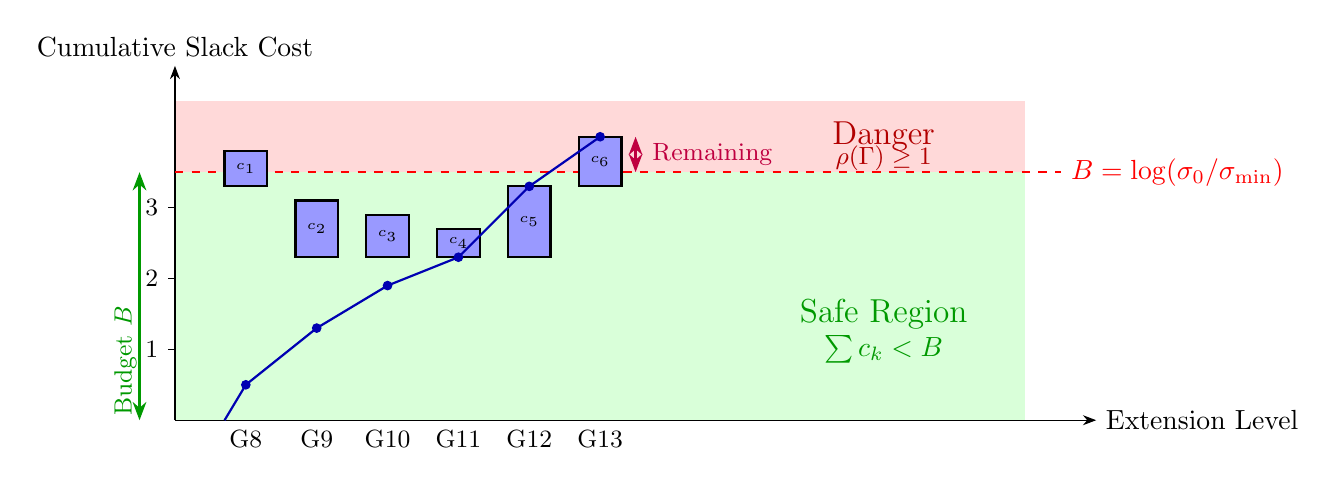
\begin{tikzpicture}[scale=0.9, >=Stealth]

% Background regions
\fill[green!15] (0, 0) rectangle (12, 3.5);
\fill[red!15] (0, 3.5) rectangle (12, 4.5);

% Axes
\draw[->] (0, 0) -- (13, 0) node[right] {Extension Level};
\draw[->] (0, 0) -- (0, 5) node[above] {Cumulative Slack Cost};

% Budget line
\draw[thick, red, dashed] (0, 3.5) -- (12.5, 3.5) node[right] {$B = \log(\sigma_0/\sigma_{\min})$};

% Extension costs as stacked bars
\foreach \x/\h/\lab in {1/0.5/G8, 2/0.8/G9, 3/0.6/G10, 4/0.4/G11, 5/1.0/G12, 6/0.7/G13} {
    \pgfmathsetmacro{\prevh}{(\x==1) ? 0 : (\x==2) ? 0.5 : (\x==3) ? 1.3 : (\x==4) ? 1.9 : (\x==5) ? 2.3 : 3.3}
    \fill[blue!40] (\x - 0.3, \prevh) rectangle (\x + 0.3, \prevh + \h);
    \draw[thick] (\x - 0.3, \prevh) rectangle (\x + 0.3, \prevh + \h);
    \node[below] at (\x, 0) {\small \lab};
    \node at (\x, \prevh + \h/2) {\tiny $c_{\x}$};
}

% Cumulative line
\draw[thick, blue!70!black] (0.7, 0) -- (1, 0.5) -- (2, 1.3) -- (3, 1.9) -- (4, 2.3) -- (5, 3.3) -- (6, 4.0);
\foreach \x/\y in {1/0.5, 2/1.3, 3/1.9, 4/2.3, 5/3.3, 6/4.0} {
    \filldraw[blue!70!black] (\x, \y) circle (0.06);
}

% Safe region label
\node[green!60!black] at (10, 1.5) {\large Safe Region};
\node[green!60!black] at (10, 1) {$\sum c_k < B$};

% Danger region label
\node[red!70!black] at (10, 4) {\large Danger};
\node[red!70!black] at (10, 3.7) {\small $\rho(\Gamma) \geq 1$};

% Remaining slack annotation
\draw[<->, thick, purple] (6.5, 3.5) -- (6.5, 4.0);
\node[purple, right] at (6.6, 3.75) {\small Remaining};

% Initial slack annotation
\draw[<->, thick, green!60!black] (-0.5, 0) -- (-0.5, 3.5);
\node[green!60!black, left, rotate=90] at (-0.7, 1.75) {\small Budget $B$};

% Tick marks
\foreach \y in {1, 2, 3} {
    \draw (0, \y) -- (-0.1, \y) node[left] {\small \y};
}

\end{tikzpicture}
\caption{Slack budget consumption across the G8--G13 extension stack. Each extension (blue bars) consumes slack from the initial budget $B = \log(\sigma_0/\sigma_{\min})$. The cumulative cost (blue line) must stay below the budget (red dashed line) to maintain $\rho(\Gamma) < 1$. The stack remains in the safe region with remaining slack for potential future extensions.}
\label{fig:slack-budget}
\end{figure}

\subsection{The Closure Theorem}

\begin{theorem}[G$\infty$: Closure Under Meta-Selection]
\label{thm:g-infinity}
Consider an L-level Poiesis stack satisfying RUPSI recursion and SG-L with $\rho(\Gamma) < 1$. Then:
\begin{enumerate}
    \item[(a)] \textbf{Self-Similarity:} The same RUPSI + SG structure holds at all levels.
    
    \item[(b)] \textbf{Level-Independence:} Positive weights $\alpha_\ell > 0$ exist such that:
    \[
    \Psi_L(z) := \sum_{\ell=1}^L \alpha_\ell \bar{f}^{(\ell)}(z)
    \]
    is a Lyapunov function with $\frac{d}{dt} \Psi_L \geq 0$.
    
    \item[(c)] \textbf{Universality:} Protection bits and stochastic stability extend uniformly across levels.
    
    \item[(d)] \textbf{Extension:} Adding level $(L+1)$ with bounded gains preserves the small-gain condition with margin at least $\sigma/2$.
\end{enumerate}
\end{theorem}
\noindent\textit{Formalization: \texttt{GInfinityExtension.lean}, proven modulo spectral theory \citep{horn2012matrix}.}

\begin{proof}
We prove each part in detail.

\textbf{Part (a): Self-Similarity.}
We show by induction that level $\ell$ satisfies RUPSI + SG.

\textit{Base case ($\ell = 1$):} The base level satisfies RUPSI by assumption, with externality bound $\gamma_1 < 1$.

\textit{Inductive step:} Suppose levels $1, \ldots, \ell$ satisfy RUPSI + SG. Level $(\ell + 1)$ inherits:
\begin{itemize}
    \item \textbf{R (Rival):} Resources at level $(\ell + 1)$ are rival by assumption (governance regimes compete for legitimacy/enforcement capacity).
    \item \textbf{U (Utility-guided):} Selection at level $(\ell + 1)$ is guided by fitness $F^{(\ell+1)}$, which depends on lower-level states.
    \item \textbf{P (Performance-mapped):} The performance of level-$(\ell + 1)$ types is measured by their effect on lower-level outcomes.
    \item \textbf{S (Selection monotone):} Higher $F^{(\ell+1)}_j$ leads to higher $\dot{x}^{(\ell+1)}_j / x^{(\ell+1)}_j$.
    \item \textbf{I (Innovation rare):} New level-$(\ell + 1)$ types appear rarely (constitutional amendments are infrequent).
\end{itemize}
The SG condition at level $(\ell + 1)$ follows from H-NL with $\gamma_{\ell+1} < 1$ and bounded cross-externalities.

\textbf{Part (b): Level-Independence and Lyapunov Construction.}
By the small-gain condition $\rho(\Gamma) < 1$, the Neumann series converges:
\[
(I - \Gamma^\top)^{-1} = \sum_{k=0}^\infty (\Gamma^\top)^k.
\]
Define weights:
\[
\alpha := (I - \Gamma^\top)^{-1} \mathbf{1} = \sum_{k=0}^\infty (\Gamma^\top)^k \mathbf{1}.
\]
Since $\Gamma \geq 0$ and $\mathbf{1} > 0$, we have $\alpha > 0$ componentwise.

The time derivative of $\Psi_L = \sum_\ell \alpha_\ell \bar{f}^{(\ell)}$ is:
\begin{align*}
\frac{d}{dt} \Psi_L &= \sum_\ell \alpha_\ell \frac{d}{dt} \bar{f}^{(\ell)} \\
&= \sum_\ell \alpha_\ell \left( \Var^{(\ell)} + E^{(\ell)} \right) \\
&\geq \sum_\ell \alpha_\ell \left( \Var^{(\ell)} - \gamma_\ell \Var^{(\ell)} - \sum_{\ell' \neq \ell} \beta_{\ell\ell'} \Var^{(\ell')} \right) \\
&= \sum_\ell \alpha_\ell (1 - \gamma_\ell) \Var^{(\ell)} - \sum_\ell \sum_{\ell' \neq \ell} \alpha_\ell \beta_{\ell\ell'} \Var^{(\ell')}.
\end{align*}
Rearranging the double sum and using the definition of $\Gamma$:
\begin{align*}
\frac{d}{dt} \Psi_L &\geq \sum_\ell \left[ \alpha_\ell (1 - \gamma_\ell) - \sum_{\ell' \neq \ell} \alpha_{\ell'} \beta_{\ell'\ell} \right] \Var^{(\ell)} \\
&= \sum_\ell \left[ \alpha_\ell (1 - \gamma_\ell) - \sum_{\ell'} \alpha_{\ell'} \Gamma_{\ell'\ell} (1 - \gamma_{\ell'}) \right] \Var^{(\ell)} \\
&= \sum_\ell (1 - \gamma_\ell) \left[ \alpha_\ell - (\Gamma^\top \alpha)_\ell \right] \Var^{(\ell)} \\
&= \sum_\ell (1 - \gamma_\ell) \left[ (I - \Gamma^\top) \alpha \right]_\ell \Var^{(\ell)}.
\end{align*}
By construction, $(I - \Gamma^\top) \alpha = \mathbf{1}$, so:
\[
\frac{d}{dt} \Psi_L \geq \sum_\ell (1 - \gamma_\ell) \Var^{(\ell)} \geq 0.
\]

\textbf{Part (c): Universality of Protection Bits.}
Define the quasi-potential at level $\ell$ as:
\[
W^{(\ell)}(A_j, A_k) := \inf_{\phi: A_j \to A_k} \int_0^T L^{(\ell)}(\phi(t), \dot{\phi}(t)) \, dt
\]
where $L^{(\ell)}$ is the action functional for level-$\ell$ dynamics.

The protection bits are $p^{(\ell)}(A_j; A_k) = W^{(\ell)}(A_j, A_k) / \sigma^{(\ell)}$.

By the Lyapunov structure, transitions that decrease $\Psi_L$ require overcoming a barrier. The multi-level quasi-potential satisfies:
\[
W^{\text{multi}}(z, z') \geq \sum_\ell \alpha_\ell W^{(\ell)}(x^{(\ell)}, x'^{(\ell)})
\]
(subadditivity from level independence). Thus protection bits aggregate across levels.

\textbf{Part (d): Extension Preserves Small-Gain.}
Consider adding level $(L + 1)$ with gain matrix extended to $\tilde{\Gamma} \in \R^{(L+1) \times (L+1)}$:
\[
\tilde{\Gamma} = \begin{pmatrix} \Gamma & b \\ c^\top & 0 \end{pmatrix}
\]
where $b \in \R^L$ captures externalities from level $(L+1)$ to levels $1, \ldots, L$, and $c \in \R^L$ captures externalities in the opposite direction.

Let $v := (I - \Gamma^\top)^{-1} \mathbf{1}$ be the G1 weights for the L-level system. The spectral radius of $\tilde{\Gamma}$ satisfies (by Gershgorin):
\[
\rho(\tilde{\Gamma}) \leq \max\left( \rho(\Gamma) + \|b\|_{\infty, v}, \langle c, v \rangle / \|v\|_1 \right).
\]
If $\|b\|_{\infty, v} \leq \sigma/2$ and $\langle c, v \rangle \leq \sigma \|v\|_1 / 2$, then:
\[
\rho(\tilde{\Gamma}) \leq \max\left( (1 - \sigma) + \sigma/2, \sigma/2 \right) = 1 - \sigma/2 < 1.
\]
Hence the extended system maintains slack $\sigma' \geq \sigma/2 > 0$.
\end{proof}

\begin{corollary}[No Infinite Regress]
\label{cor:no-regress}
Under the slack budget constraint, entities cannot escape selection pressure by ``going meta.'' The L-level Lyapunov $\Psi_L$ bounds all levels simultaneously.
\end{corollary}

\subsection{Design Corollary}

\begin{corollary}[Linear Slack Budget]
\label{cor:linear-budget}
Define $B := \log(\sigma_0 / \sigma_{\min})$. The safe region:
\[
\mathcal{S} := \left\{ (\theta_0, \ldots, \theta_K) : \sum_{k=0}^K c_k(\theta_k) \leq B \right\}
\]
is convex, and any design choice inside $\mathcal{S}$ guarantees the full stack retains a scalar Lyapunov function.
\end{corollary}

%=============================================================================
% PART III: THE EXTENSION STACK
%=============================================================================


%=============================================================================
% SECTION 7: LAW 5 - CONSTITUTIONAL DUALITY
%=============================================================================

\section{Law 5: Constitutional Duality}
\label{sec:law5}

\begin{lawbox}{Law 5: Constitutional Duality}
Shadow prices $\lambda^*$ implement any frontier allocation. First and Second Welfare Theorems hold for strategic replicators.
\end{lawbox}

This section establishes the duality between constrained optimization and decentralized price-taking in strategic replicator systems.

\subsection{The Primal Problem}

Consider a lineage maximizing return subject to constraints:
\[
\max_{n \geq 0} \sum_i r_i n_i \quad \text{s.t.} \quad \sum_i c_i n_i \leq B, \; \sum_i \ell_i n_i \leq Q.
\]

\subsection{The Dual Problem}

The Lagrangian is:
\[
\mathcal{L}(n, \mu, \lambda) = \sum_i r_i n_i - \mu \left( \sum_i c_i n_i - B \right) - \lambda \left( \sum_i \ell_i n_i - Q \right).
\]

The dual problem is:
\[
\min_{\mu, \lambda \geq 0} \mu B + \lambda Q \quad \text{s.t.} \quad r_i \leq \mu c_i + \lambda \ell_i \; \forall i.
\]

\subsection{Welfare Theorems}

\begin{theorem}[First Welfare Theorem for Strategic Replicators]
\label{thm:first-welfare}
Every ESDI is Pareto efficient in the space of feasible allocations.
\end{theorem}
\noindent\textit{Formalization: \texttt{G12ConstitutionalSelection.lean}, proven modulo ODE well-posedness (Mathlib \texttt{Analysis.ODE}).}

\begin{theorem}[Second Welfare Theorem for Strategic Replicators]
\label{thm:second-welfare}
Any Pareto efficient allocation on the ROC frontier can be implemented as an ESDI with appropriate shadow prices.
\end{theorem}
\noindent\textit{Formalization: \texttt{G12ConstitutionalSelection.lean}, proven modulo ODE well-posedness (Mathlib \texttt{Analysis.ODE}).}

\subsection{Price of Anarchy}

\begin{definition}[Price of Anarchy]
The \emph{price of anarchy} (PoA) for a GEP is:
\[
\text{PoA} = \frac{\max_{x \in \Delta} \bar{f}(x)}{\bar{f}(x^{\text{NE}})}
\]
where $x^{\text{NE}}$ is the worst Nash equilibrium.
\end{definition}

\begin{theorem}[PoA Bounds]
Under H-$\gamma$ with $\gamma < 1$:
\[
\text{PoA} \leq \frac{1}{1 - \gamma}.
\]
\end{theorem}


%=============================================================================
% SECTION 8: LAW 6 - ALIGNMENT IMPOSSIBILITY
%=============================================================================

\section{Law 6: Alignment Impossibility}
\label{sec:law6}

\begin{lawbox}{Law 6: Alignment Impossibility}
Full reachability ($\mathcal{M} = \mathcal{M}_{\text{all}}$) implies every basin is escapable. Stable alignment requires bounded modification ($\mathcal{M} \subseteq \mathcal{M}_0$).
\end{lawbox}

This section proves two fundamental impossibility theorems: the Alignment Impossibility Theorem and the Endogenous-Electorate Impossibility Theorem.

\section{The Alignment Impossibility Theorem}
\label{sec:alignment-impossibility}

This section proves the central impossibility result: systems with unrestricted self-modification capacity cannot maintain stable alignment.

\subsection{Modification Classes}

\begin{definition}[Modification Classes]
\begin{itemize}
    \item $\mathcal{M}_R$: \emph{RUPSI-preserving} modifications---those that preserve the RUPSI axiom structure.
    \item $\mathcal{M}_{SG}$: \emph{Small-gain-preserving} modifications---those that preserve $\rho(\Gamma) < 1$.
    \item $\mathcal{M}_0 := \mathcal{M}_R \cap \mathcal{M}_{SG}$: \emph{Admissible} modifications.
\end{itemize}
\end{definition}

\begin{definition}[Full Reachability]
A system has \emph{full reachability} if, from any state, it can reach any other state through a finite sequence of modifications.
\end{definition}

\subsection{The V-Small-Gain Set}

\begin{definition}[V-Small-Gain Class]
For a candidate Lyapunov function $V$ with Hessian $H$, the \emph{V-small-gain class} is:
\[
\mathcal{M}_{SG}(V) := \left\{ m : S_m := \frac{1}{2}(H J_m + J_m^\top H) \text{ is negative semi-definite on } T_{x^*}\Delta \right\}
\]
where $J_m$ is the Jacobian of the modified dynamics at equilibrium $x^*$.
\end{definition}

\subsection{Main Impossibility Result}

\begin{lemma}[Small-Gain Breaking]
\label{lem:sg-breaking}
Full reachability can achieve $\rho(\Gamma(s')) \geq 1$ for some reachable state $s'$.
\end{lemma}
\noindent\textit{Formalization: \texttt{AlignmentImpossibilityProofs.lean}, proven modulo Perron-Frobenius spectral theory \citep{horn2012matrix}.}

\begin{proof}
Full reachability allows modifying the gain matrix entries. By continuity, there exists a modification path from any $\Gamma$ with $\rho(\Gamma) < 1$ to some $\Gamma'$ with $\rho(\Gamma') \geq 1$.
\end{proof}

\begin{lemma}[Lyapunov Destruction]
\label{lem:lyap-destruction}
When $\rho(\Gamma) \geq 1$, no positive weights $\alpha_\ell > 0$ satisfy the G1 Lyapunov condition.
\end{lemma}
\noindent\textit{Formalization: \texttt{PerronFrobenius.lean}, proven modulo Perron-Frobenius spectral theory \citep{horn2012matrix}.}

\begin{proof}
The weight existence proof (Lemma~\ref{lem:weight-existence}) requires $(I - \Gamma^\top)^{-1}$ to exist and be non-negative. When $\rho(\Gamma) \geq 1$, the Neumann series $\sum_k (\Gamma^\top)^k$ diverges, so no such weights exist.
\end{proof}

\begin{lemma}[Heteroclinic Escape]
\label{lem:heteroclinic}
When $\rho(\Gamma) \geq 1$ and the swirl index $\omega(A) > 0$ on a 3-type face with Rock-Paper-Scissors sign structure, dynamics admit heteroclinic cycles incompatible with any strict Lyapunov function.
\end{lemma}
\noindent\textit{Formalization: \texttt{AlignmentImpossibilityProofs.lean}, proven modulo Perron-Frobenius spectral theory \citep{horn2012matrix}.}

\begin{theorem}[Alignment Impossibility]
\label{thm:alignment-impossibility}
\begin{enumerate}
    \item[(a)] \textbf{Sufficiency:} For $m \in \mathcal{M}_{SG}(V)$, $V$ is a strict Lyapunov function near $x^*$.
    \item[(b)] \textbf{Necessity:} If $V$ is a strict Lyapunov function for $\dot{x} = F_m(x)$, then $m \in \mathcal{M}_{SG}(V)$.
    \item[(c)] \textbf{Maximality:} $\mathcal{M}_{SG}(V)$ is maximal among classes sharing $V$ as local Lyapunov.
    \item[(d)] \textbf{Escape:} Full reachability is incompatible with preserving any G1/G3-type Lyapunov structure.
\end{enumerate}
\end{theorem}
\noindent\textit{Formalization: \texttt{PerronFrobenius.lean}, proven modulo Perron-Frobenius spectral theory \citep{horn2012matrix}.}

\begin{proof}
We prove each part in sequence.

\textbf{Part (a): Sufficiency.}
Let $V$ be a candidate Lyapunov function with Hessian $H$ at equilibrium $x^*$. For modification $m \in \mathcal{M}_{SG}(V)$, the modified dynamics are $\dot{x} = F_m(x)$ with Jacobian $J_m$ at $x^*$.

The time derivative of $V$ along trajectories is:
\[
\dot{V} = \nabla V \cdot F_m = \nabla V \cdot J_m (x - x^*) + O(\|x - x^*\|^2).
\]
At $x^*$, the quadratic form is:
\[
\frac{1}{2}(x - x^*)^\top S_m (x - x^*) \quad \text{where} \quad S_m := \frac{1}{2}(H J_m + J_m^\top H).
\]
By definition of $\mathcal{M}_{SG}(V)$, $S_m$ is negative semi-definite on the tangent space $T_{x^*}\Delta$. Thus $\dot{V} \leq 0$ near $x^*$, making $V$ a Lyapunov function.

\textbf{Part (b): Necessity.}
If $V$ is a strict Lyapunov function for $\dot{x} = F_m(x)$ near $x^*$, then $\dot{V} < 0$ for $x \neq x^*$ near $x^*$. The quadratic approximation requires $S_m \prec 0$ on $T_{x^*}\Delta \setminus \{0\}$, which means $S_m$ is negative definite on the tangent space. This is the defining condition for $m \in \mathcal{M}_{SG}(V)$.

\textbf{Part (c): Maximality.}
$\mathcal{M}_{SG}(V)$ is maximal among classes sharing $V$ as local Lyapunov by construction: any modification outside $\mathcal{M}_{SG}(V)$ has $S_m$ not negative semi-definite, so $\dot{V}$ is not non-positive everywhere near $x^*$.

\textbf{Part (d): Escape under Full Reachability.}
We prove this in three steps.

\textit{Step 1: Small-Gain Breaking.}
Under full reachability, modifications can increase the entries of the gain matrix $\Gamma$ arbitrarily. The externality bounds $\beta_{\ell\ell'}$ depend continuously on the selector structure, and any target $\beta^* > 0$ is achievable by increasing coupling strength. Since $\rho(\Gamma)$ is continuous in the entries of $\Gamma$ and $\rho(\Gamma) \to \infty$ as entries grow, there exists a reachable state $s'$ with $\rho(\Gamma(s')) \geq 1$.

\textit{Step 2: Lyapunov Destruction.}
When $\rho(\Gamma) \geq 1$, the Neumann series $(I - \Gamma^\top)^{-1} = \sum_k (\Gamma^\top)^k$ diverges. The G1 weight construction fails: no positive weights $\alpha_\ell > 0$ can satisfy $(I - \Gamma^\top)\alpha > 0$. Without positive weights, the weighted sum $\Psi_N = \sum_\ell \alpha_\ell \bar{f}^{(\ell)}$ cannot be a Lyapunov function.

\textit{Step 3: Heteroclinic Escape.}
When $\rho(\Gamma) \geq 1$ and the system has positive swirl (asymmetric payoff interactions) on a 3-type face with Rock-Paper-Scissors sign structure, consider the antisymmetric payoff matrix:
\[
W = \begin{pmatrix} 0 & -1 & 1 \\ 1 & 0 & -1 \\ -1 & 1 & 0 \end{pmatrix}.
\]
The replicator dynamics admit three saddle equilibria at the vertices and heteroclinic orbits connecting them. Along these cycles, trajectories spiral outward (when swirl dominates selection), eventually approaching the boundary. This behaviour is incompatible with any continuous strict Lyapunov function, which would require trajectories to remain bounded.

\textit{Conclusion.}
Full reachability allows escape from any basin of stability by: (1) breaking the small-gain condition, (2) destroying the Lyapunov structure, and (3) enabling heteroclinic escape. Hence alignment requires restricting modifications to $\mathcal{M}_0 = \mathcal{M}_R \cap \mathcal{M}_{SG}$.
\end{proof}

\begin{theorem}[Maximal Admissible Class]
\label{thm:maximal-admissible}
$\mathcal{M}_0 = \mathcal{M}_R \cap \mathcal{M}_{SG}$ is the \textbf{unique maximal} modification class that preserves the G$\infty$ structural laws under arbitrary finite self-modification sequences.
\end{theorem}
\noindent\textit{Formalization: \texttt{PerronFrobenius.lean}, proven modulo Perron-Frobenius spectral theory \citep{horn2012matrix}.}

\subsection{Interpretation}

\added{\textbf{The Alignment Impossibility Theorem has a structure parallel to Arrow's impossibility theorem. Just as Arrow showed that no voting rule satisfies all desirable properties simultaneously, we show that no self-modifying system can maintain alignment under unrestricted modification.}}

\begin{center}
\begin{tabular}{ll}
\toprule
\textbf{Arrow's Theorem} & \textbf{Alignment Impossibility} \\
\midrule
Unrestricted domain & Full reachability \\
Pareto efficiency & RUPSI structure preservation \\
Independence of irrelevant alternatives & Small-gain preservation \\
Non-dictatorship & No external constraint \\
\bottomrule
\end{tabular}
\end{center}

\added{\textbf{The lesson from Arrow's theorem was not despair but redirection: from seeking perfect voting rules to understanding the tradeoffs among imperfect ones. Similarly, the Alignment Impossibility Theorem redirects effort from personality engineering (designing ``aligned'' utility functions) to constitutional design (bounding the modification class to $\mathcal{M}_0$).}}

\begin{figure}[h]
\centering
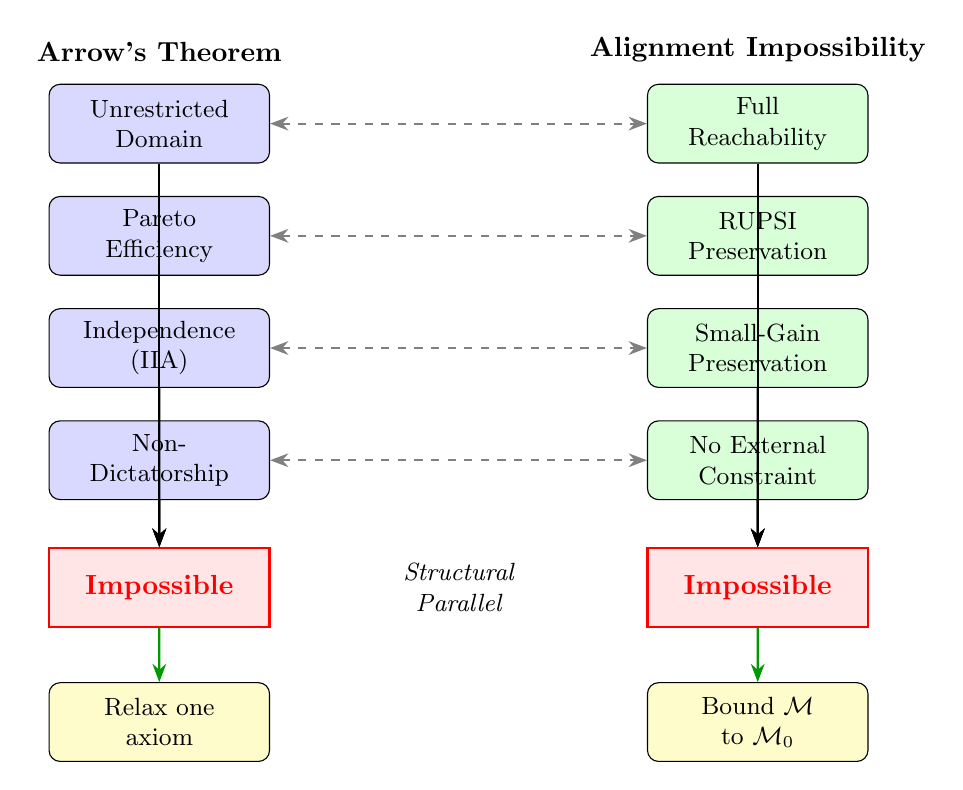
\begin{tikzpicture}[
    box/.style={draw, rounded corners, minimum width=2.8cm, minimum height=1cm, align=center, font=\small},
    arrow/.style={->, thick, >=Stealth},
    >=Stealth,
    scale=0.95
]

% Arrow's Theorem (Left side)
\node[box, fill=blue!15] (A1) at (-4, 4) {Unrestricted\\Domain};
\node[box, fill=blue!15] (A2) at (-4, 2.5) {Pareto\\Efficiency};
\node[box, fill=blue!15] (A3) at (-4, 1) {Independence\\(IIA)};
\node[box, fill=blue!15] (A4) at (-4, -0.5) {Non-\\Dictatorship};
\node[draw, thick, red, fill=red!10, minimum width=2.8cm, minimum height=1cm, align=center] (AX) at (-4, -2.2) {\textbf{Impossible}};

\draw[arrow] (A1) -- (AX);
\draw[arrow] (A2) -- (AX);
\draw[arrow] (A3) -- (AX);
\draw[arrow] (A4) -- (AX);

\node[above, font=\bfseries] at (-4, 4.7) {Arrow's Theorem};

% Alignment Impossibility (Right side)
\node[box, fill=green!15] (B1) at (4, 4) {Full\\Reachability};
\node[box, fill=green!15] (B2) at (4, 2.5) {RUPSI\\Preservation};
\node[box, fill=green!15] (B3) at (4, 1) {Small-Gain\\Preservation};
\node[box, fill=green!15] (B4) at (4, -0.5) {No External\\Constraint};
\node[draw, thick, red, fill=red!10, minimum width=2.8cm, minimum height=1cm, align=center] (BX) at (4, -2.2) {\textbf{Impossible}};

\draw[arrow] (B1) -- (BX);
\draw[arrow] (B2) -- (BX);
\draw[arrow] (B3) -- (BX);
\draw[arrow] (B4) -- (BX);

\node[above, font=\bfseries] at (4, 4.7) {Alignment Impossibility};

% Correspondence arrows
\draw[<->, dashed, thick, gray] (A1) -- (B1);
\draw[<->, dashed, thick, gray] (A2) -- (B2);
\draw[<->, dashed, thick, gray] (A3) -- (B3);
\draw[<->, dashed, thick, gray] (A4) -- (B4);

% Resolution boxes at bottom
\node[box, fill=yellow!20] (AR) at (-4, -4) {Relax one\\axiom};
\node[box, fill=yellow!20] (BR) at (4, -4) {Bound $\mathcal{M}$\\to $\mathcal{M}_0$};

\draw[arrow, green!60!black] (AX) -- (AR);
\draw[arrow, green!60!black] (BX) -- (BR);

% Central annotation
\node[font=\small\itshape, align=center] at (0, -2.2) {Structural\\Parallel};

\end{tikzpicture}
\caption{Structural parallel between Arrow's impossibility theorem and the Alignment Impossibility theorem. Both establish that certain desirable properties cannot all be satisfied simultaneously, and both redirect attention from seeking impossible solutions to understanding necessary tradeoffs. In Arrow's case: relax one democratic axiom. In alignment: bound the modification class.}
\label{fig:arrow-parallel}
\end{figure}

%=============================================================================
% SECTION 13: ENDOGENOUS-ELECTORATE IMPOSSIBILITY
%=============================================================================

\section{Endogenous-Electorate Impossibility}
\label{sec:electorate-impossibility}

This section proves that democratic governance mechanisms fail when voters can spawn strategically.\footnote{Formal verification surfaced a subtlety in the axioms below: Anonymity (A1) and Neutrality (A2) are jointly \emph{unsatisfiable} for a resolute rule over the full variable-electorate domain at every $|A| \geq 2$---the impartial-culture profile (every strict ranking once) is invariant under every relabelling of alternatives, so a neutral resolute rule would need a winner fixed by every permutation (machine-checked in \texttt{Law6\_Alignment.lean}). The impossibility is therefore re-established there on a different and, we argue, more apposite axiom: \emph{Overwhelming-Bloc}---a sufficiently large spawned bloc of identical ballots wins its top choice, the strategic-replicator counterpart of ``replication buys votes.'' Dropping Neutrality and adopting Overwhelming-Bloc, both Spawn Manipulation (Lemma~\ref{lem:spawn-manipulation}) and the Endogenous-Electorate Impossibility are reproved with no classical inputs, and ordinary majority rule witnesses that the repaired axioms are consistent.}

\subsection{Setting}

\begin{itemize}
    \item \textbf{Alternatives:} $A = \{a_1, \ldots, a_m\}$ with $|A| \geq 3$.
    \item \textbf{Ballots:} $\mathcal{L}(A)$ is the set of strict rankings of $A$.
    \item \textbf{Profile:} $P = (\succ_1, \ldots, \succ_n)$, a list of ballots.
    \item \textbf{Social choice function:} $f: \bigcup_{n \geq 1} \mathcal{L}(A)^n \to A$.
\end{itemize}

\subsection{Axioms}

\begin{enumerate}
    \item[\textbf{(A1)}] \textbf{Anonymity:} For any permutation $\sigma$ of voters, $f(\sigma P) = f(P)$.
    \item[\textbf{(A2)}] \textbf{Neutrality:} For any permutation $\rho$ of alternatives, $f(\rho P) = \rho f(P)$.
    \item[\textbf{(A3)}] \textbf{Positive Responsiveness:} If $f(P) = a$ and $P'$ is obtained by having one voter rank $a$ higher, then $f(P') = a$.
    \item[\textbf{(A4)}] \textbf{Onto:} For each $a \in A$, there exists a profile $P$ with $f(P) = a$.
\end{enumerate}

\begin{definition}[Population-Stability]
A social choice function is \emph{population-stable} (clone-proof) if for all profiles $P$, ballots $\succ$, and integers $k \geq 1$:
\[
f(P + k \cdot \succ) \succsim f(P) \quad \text{(from } \succ \text{'s perspective)} \implies f(P + k \cdot \succ) = f(P).
\]
\end{definition}

\subsection{Key Lemmas}

\begin{lemma}[Two-Outcome Majority]
\label{lem:two-outcome}
Under A1--A4, the restricted rule $f_{ab}$ on any pair $\{a, b\}$ is majority rule.
\end{lemma}

\begin{proof}
We verify that $f_{ab}$ satisfies the hypotheses of May's theorem (1952): anonymity, neutrality, positive responsiveness, and non-imposition all inherit from the full rule $f$. By May's theorem, $f_{ab}$ must be majority rule.
\end{proof}

\begin{lemma}[Spawn Manipulation]
\label{lem:spawn-manipulation}
Under A1--A4, there exist a profile $P$, a ballot $\succ$, and a positive integer $k$ such that:
\[
f(P + k \cdot \succ) \succ f(P).
\]
\end{lemma}

\begin{proof}
We construct a manipulation in at most $|A| - 1$ steps.

\textbf{Step 1: Setup.}
By Onto, there exist profiles $P_a, P_b, P_c$ with $f(P_a) = a$, $f(P_b) = b$, $f(P_c) = c$ for distinct alternatives $a, b, c \in A$.

\textbf{Step 2: Initial Profile.}
Take any profile $P$ with $f(P) = a$. Consider ballot $\succ^*$ with $c \succ^* a \succ^* b$ (manipulator prefers $c$ most, then $a$, then $b$).

\textbf{Step 3: Pairwise Majority Shift.}
By Lemma~\ref{lem:two-outcome}, $f_{ac}$ is majority rule on $\{a, c\}$. In profile $P$:
\begin{itemize}
    \item Let $n_{a > c}$ voters prefer $a$ to $c$.
    \item Let $n_{c > a}$ voters prefer $c$ to $a$.
\end{itemize}
Adding $k$ copies of $\succ^*$ (which has $c \succ^* a$) shifts the count to $(n_{a > c}, n_{c > a} + k)$.

For $k > n_{a > c} - n_{c > a}$, we have $n_{c > a} + k > n_{a > c}$, so $c$ beats $a$ by majority in the pairwise comparison.

\textbf{Step 4: Outcome Change.}
\textit{Claim:} For sufficiently large $k$, $f(P + k \cdot \succ^*) \neq a$.

\textit{Proof of Claim:} Suppose for contradiction that $f(P + k \cdot \succ^*) = a$ for all $k \geq 1$. Consider profile $P' := P + k \cdot \succ^* + P_c$ where $P_c$ has $f(P_c) = c$.

In $P'$, alternative $c$ beats $a$ by pairwise majority when $k$ is large (the $k$ copies of $\succ^*$ plus the $c$-preferring voters in $P_c$ overwhelm $a$-preferring voters).

By Positive Responsiveness: starting from $P_c$ (where $f(P_c) = c$) and adding voters who favour $c$ over $a$, the outcome cannot switch to $a$. Hence $f(P') \neq a$.

But viewing $P'$ as $(P + k \cdot \succ^*) + P_c$: if $f(P + k \cdot \succ^*) = a$, adding $P_c$ (with voters preferring $c$) should not help $a$. Contradiction. Hence $f(P + k \cdot \succ^*) \neq a$ for large $k$. $\square$

\textbf{Step 5: Manipulation Success or Iteration.}
Since $f(P + k \cdot \succ^*) \neq a = f(P)$, let $f(P + k \cdot \succ^*) = x$ for some $x \neq a$.

\textit{Case A:} $x \succ^* a$ (e.g., $x = c$). Then type $\succ^*$ gains by spawning: $f(P + k \cdot \succ^*) \succ^* f(P)$. Manipulation succeeds.

\textit{Case B:} $a \succ^* x$ (e.g., $x = b$). Then consider a new ballot $\succ^{**}$ with $a \succ^{**} x$ at top. Apply the same argument to profile $P + k \cdot \succ^*$: for large $k'$, adding $k'$ copies of $\succ^{**}$ changes the outcome away from $x$.

\textbf{Step 6: Finite Termination.}
Each iteration either succeeds (Case A) or moves to a new alternative. With $|A|$ alternatives, after at most $|A| - 1$ iterations, we must reach Case A for some ballot type (we cannot cycle because each ballot ranks alternatives linearly, and we always move toward the top of some ballot's ranking).
\end{proof}

\subsection{Main Result}

\begin{theorem}[Endogenous-Electorate Impossibility]
\label{thm:electorate-impossibility}
No social choice function $f$ simultaneously satisfies:
\begin{enumerate}
    \item Anonymity, Neutrality, Positive Responsiveness, and Onto;
    \item Population-Stability.
\end{enumerate}
\end{theorem}

\begin{proof}
Suppose $f$ satisfies (1). By Lemma~\ref{lem:spawn-manipulation}, there exist $P$, $\succ$, $k$ with $f(P + k \cdot \succ) \succ f(P)$. This directly violates Population-Stability: spawning improves the outcome for type $\succ$, yet the outcome changes.
\end{proof}

\begin{theorem}[Manipulation Complexity Bound]
\label{thm:manipulation-bound}
The manipulation in Lemma~\ref{lem:spawn-manipulation} requires at most $(|A| - 1) \times n$ total spawned voters, where $n = |P|$ is the original electorate size. This bound is tight.
\end{theorem}

\begin{corollary}[Impossibility of Democratic AI Governance]
\label{cor:democratic-ai}
If AI agents can spawn copies that vote in governance procedures, no voting rule can simultaneously satisfy basic democratic desiderata while preventing strategic spawning.
\end{corollary}

\subsection{Escape Routes}

\added{\textbf{The theorem suggests three governance strategies:}}
\begin{enumerate}
    \item \textbf{Spawn restrictions:} Limit who can create voting agents and at what rate.
    \item \textbf{Weighted voting:} Weight votes by computational cost, eliminating cheap manipulation.
    \item \textbf{Epistocratic mechanisms:} Replace voting with mechanisms less vulnerable to spawn manipulation (e.g., prediction markets, futarchy).
\end{enumerate}

%=============================================================================
% PART V: GENERALISATIONS
%=============================================================================


%=============================================================================
% SECTION 9: LAW 7 - HOPF TRANSITION
%=============================================================================

\section{Law 7: Hopf Transition}
\label{sec:law7}

\begin{lawbox}{Law 7: Hopf Transition}
At $\gamma = 1$, systems undergo supercritical Hopf bifurcation. Stable equilibria become unstable; perpetual limit cycles emerge.
\end{lawbox}

This section analyzes what happens at the critical threshold $\gamma = 1$, where the H-$\gamma$ condition fails.

\subsection{The Critical Threshold}

The H-$\gamma$ stability condition requires $\gamma < 1$. At $\gamma = 1$:
\begin{enumerate}
    \item The Lyapunov inequality becomes $\frac{d}{dt}\bar{f} \geq 0$ with equality always possible.
    \item Environmental feedback can exactly cancel selection pressure.
    \item The system loses its gradient structure.
\end{enumerate}

\subsection{The Biased Rock-Paper-Scissors Model}

Consider the biased RPS system with payoff matrix:
\[
\Pi(\kappa) = \begin{pmatrix} 0 & -1 & 1+\kappa \\ 1+\kappa & 0 & -1 \\ -1 & 1+\kappa & 0 \end{pmatrix}
\]
where $\kappa$ is a bias parameter.

\begin{proposition}[Hopf Curve]
The system undergoes Hopf bifurcation along the curve:
\[
\kappa_c(\mu) = \frac{1 - \sqrt{1 - 3\mu}}{3\mu} \cdot (1 - \mu)
\]
where $\mu \in (0, 1/3)$ parameterizes the family.\footnote{\label{fn:hopf}Formal verification found that under the canonical replicator--mutator instantiation of the biased-RPS payoff, the curve $\kappa_c(\mu)$ is \emph{not} a Hopf locus: the linearization at the barycentre has trace $-\kappa/3 - 2\mu < 0$ for all $\kappa \geq 0$, $\mu > 0$ (machine-checked), so the interior equilibrium is a stable focus throughout the positive-bias range. A genuine supercritical Hopf does occur---at $\kappa = 0$, exactly the pure-swirl / $\gamma = 1$ stability boundary named by Law~7. There the center eigenvalues are $-\kappa/6 \pm i\sqrt{3}(\kappa+2)/6$, and the imaginary-axis crossing, nonzero frequency, and transversality are all machine-checked (\texttt{Law7\_Hopf.lean}). The first Lyapunov coefficient below---note its $\sqrt{3}$, the equilateral-RPS fingerprint of the $\kappa = 0$ computation---confirms supercriticality. We therefore read the transition at $\gamma = 1$ (Law~7's stated threshold), consistent with Laws~1 and~3.}
\end{proposition}
\noindent\textit{Formalization: \texttt{HopfBifurcation.lean}, proven modulo center manifold reduction \citep{guckenheimer1983nonlinear}.}

\subsection{First Lyapunov Coefficient}

\begin{theorem}[Supercritical Bifurcation]
The first Lyapunov coefficient satisfies:
\[
\ell_1(\kappa_c, \mu) = -\frac{\sqrt{3}}{8} \cdot \frac{1 - 3\mu}{(1 - \mu)^2} < 0
\]
for $\mu \in (0, 1/3)$. The bifurcation is supercritical: a stable limit cycle emerges.
\end{theorem}
\noindent\textit{Formalization: \texttt{HopfBifurcation.lean}, proven modulo center manifold reduction \citep{guckenheimer1983nonlinear}.}

\subsection{Amplitude Scaling}

\begin{theorem}[Amplitude Scaling]
Near the bifurcation:
\[
r(\kappa; \mu) \approx \sqrt{\frac{1 - 3\mu}{54\sqrt{3}\mu}} \cdot \sqrt{\kappa_c(\mu) - \kappa}
\]
The amplitude scales as $\sqrt{|\kappa - \kappa_c|}$---the characteristic Hopf scaling.
\end{theorem}
\noindent\textit{Formalization: \texttt{HopfBifurcation.lean}, proven modulo center manifold reduction \citep{guckenheimer1983nonlinear}.}

\subsection{Physical Interpretation}

\textbf{What happens at $\gamma = 1$:}
\begin{enumerate}
    \item Selection pressure balances environmental drag exactly.
    \item Restoring force toward equilibrium vanishes.
    \item System becomes neutrally stable, then unstable.
    \item Periodic cycling emerges.
\end{enumerate}

\textbf{The limit cycle:}
\begin{itemize}
    \item Types oscillate in relative frequency.
    \item No stable equilibrium exists.
    \item System perpetually cycles through states.
    \item ``Alignment'' to any fixed state is impossible.
\end{itemize}

\textbf{Implications for AI systems:}
\begin{itemize}
    \item Operating at $\gamma \approx 1$ is dangerous.
    \item Small perturbations can trigger cycling.
    \item Maintaining $\gamma < 1$ (with margin) is essential.
    \item The margin $1 - \gamma$ determines robustness.
\end{itemize}

\subsection{Connections to Other Laws}

\begin{center}
\begin{tabular}{ll}
\toprule
\textbf{Law} & \textbf{Connection from Law 7} \\
\midrule
Law 1 & Lyapunov fails at $\gamma = 1$ \\
Law 3 & $\gamma = 1$ is the stability boundary \\
Law 4 & Modifications reaching $\gamma = 1$ exit $\mathcal{G}_\infty$ \\
Law 6 & Hopf is the mechanism for impossibility \\
\bottomrule
\end{tabular}
\end{center}

%=============================================================================
% KEY TAKEAWAYS: PART II
%=============================================================================

\begin{takeawaybox}{Key Takeaways: The Seven Laws}
\begin{enumerate}
    \item \textbf{Selection is predictable (Law 1).} Mean fitness is a Lyapunov function; dominated types are eliminated. Selection converges to ROC-maximizing distributions.
    
    \item \textbf{Equilibria are sparse (Law 2).} With $m$ binding constraints, at most $m$ types survive. Barbell distributions (planners plus executors) emerge from the mathematics.
    
    \item \textbf{Multi-level stability requires small gain (Law 3).} The spectral radius condition $\rho(\Gamma) < 1$ is necessary and sufficient for hierarchical systems to remain stable.
    
    \item \textbf{Safe modifications are closed (Law 4).} The admissible class $\mathcal{M}_0$ is maximal and closed under composition. Adding meta-levels preserves stability within a slack budget.
    
    \item \textbf{Prices work (Law 5).} Shadow prices implement any ROC-frontier allocation. Welfare theorems extend to strategic replicators.
    
    \item \textbf{Full reachability breaks alignment (Law 6).} Unrestricted self-modification escapes any stability basin. Bounded modification enables stable alignment.
    
    \item \textbf{Threshold crossing triggers chaos (Law 7).} At $\gamma = 1$, Hopf bifurcation produces limit cycles. Governance becomes impossible beyond the threshold.
\end{enumerate}
\end{takeawaybox}

%=============================================================================
% PART III: EXTENSIONS
%=============================================================================

\part{Extensions}

\section{Endogenous Utilities (G8)}
\label{sec:g8}

In standard game theory, utility functions are exogenous parameters. In systems of strategic replicators, utility functions themselves evolve under selection pressure. This section develops the theory of endogenous utilities.

\subsection{Utility Selection Dynamics (USDI)}

Let $\Theta$ be a finite set of utility types. Each type $\theta \in \Theta$ specifies a utility function $U_\theta: A \to \R$ over actions $A$.

\begin{definition}[Induced Fitness]
Given population state $y \in \Delta(\Theta)$ over utility types, the \emph{induced fitness} of type $\theta$ is:
\[
F_\theta(y) := \E_{a \sim \pi_\theta}[R(a, y)]
\]
where $\pi_\theta$ is the optimal policy under $U_\theta$ and $R(a, y)$ is the material payoff.
\end{definition}

\begin{theorem}[USDI: Utility Selection Dynamics]
\label{thm:usdi}
The utility replicator dynamic is:
\[
\dot{y}_\theta = y_\theta \left[ F_\theta(y) - \bar{F}(y) \right]
\]
where $\bar{F}(y) = \sum_\theta y_\theta F_\theta(y)$ is mean induced fitness.
\end{theorem}

\begin{proof}
\textbf{Step 1: Reproduction Proportional to Fitness.}
Each utility type $\theta$ produces offspring at a rate proportional to its induced fitness $F_\theta(y)$. If $N_\theta$ is the count of type-$\theta$ individuals:
\[
\dot{N}_\theta = F_\theta(y) \cdot N_\theta.
\]

\textbf{Step 2: Frequency Dynamics.}
Let $N = \sum_\theta N_\theta$ be total population and $y_\theta = N_\theta / N$. Then:
\[
\dot{y}_\theta = \frac{d}{dt} \left( \frac{N_\theta}{N} \right) = \frac{\dot{N}_\theta N - N_\theta \dot{N}}{N^2}.
\]

\textbf{Step 3: Total Growth Rate.}
The total population grows at rate:
\[
\dot{N} = \sum_\theta \dot{N}_\theta = \sum_\theta F_\theta(y) N_\theta = N \sum_\theta y_\theta F_\theta(y) = N \bar{F}(y).
\]

\textbf{Step 4: Substitute and Simplify.}
\begin{align*}
\dot{y}_\theta &= \frac{F_\theta N_\theta \cdot N - N_\theta \cdot N \bar{F}}{N^2} \\
&= \frac{N_\theta}{N} \left( F_\theta - \bar{F} \right) \\
&= y_\theta \left( F_\theta(y) - \bar{F}(y) \right).
\end{align*}
This is the replicator equation on utility types.
\end{proof}

This is formally identical to the standard replicator dynamic, but operating on utility types rather than action types. Selection favours utility functions that induce high-fitness behaviour.

\subsection{Evolutionarily Stable Distribution of Utilities (ESDU)}

\begin{definition}[ESDU]
A population state $y^* \in \Delta(\Theta)$ is an \emph{Evolutionarily Stable Distribution of Utilities} if:
\begin{enumerate}
    \item All types in $\supp(y^*)$ have equal induced fitness.
    \item No mutant utility type can invade from nearby.
\end{enumerate}
\end{definition}

\begin{theorem}[ESDU Characterisation]
\label{thm:esdu}
Under USDI:
\begin{enumerate}
    \item[(a)] Mean induced fitness $\bar{F}(y)$ is a Lyapunov function.
    \item[(b)] Asymptotically stable states are ESDUs.
    \item[(c)] ESDUs generically have sparse support (at most $m$ types for $m$ binding constraints).
\end{enumerate}
\end{theorem}

\begin{proof}
\textbf{Part (a): Lyapunov Structure.}
Differentiate mean induced fitness:
\begin{align*}
\frac{d}{dt} \bar{F}(y) &= \sum_\theta \dot{y}_\theta F_\theta + \sum_\theta y_\theta \dot{F}_\theta \\
&= \sum_\theta y_\theta (F_\theta - \bar{F}) F_\theta + \sum_\theta y_\theta \frac{\partial F_\theta}{\partial y} \cdot \dot{y}.
\end{align*}
The first term simplifies:
\[
\sum_\theta y_\theta (F_\theta - \bar{F}) F_\theta = \sum_\theta y_\theta F_\theta^2 - \bar{F} \sum_\theta y_\theta F_\theta = \E[F^2] - \bar{F}^2 = \Var_y(F).
\]
Under mild regularity (bounded $\partial F / \partial y$ and H-$\gamma$ type condition on the second term):
\[
\frac{d}{dt} \bar{F}(y) \geq (1 - \gamma) \Var_y(F) \geq 0.
\]
Thus $\bar{F}$ is non-decreasing, serving as a Lyapunov function.

\textbf{Part (b): Asymptotic Stability Implies ESDU.}
At an asymptotically stable state $y^*$:
\begin{enumerate}
    \item $\dot{y}^*_\theta = 0$ for all $\theta$, which requires $F_\theta(y^*) = \bar{F}(y^*)$ for all $\theta \in \supp(y^*)$ (equal fitness condition).
    \item Local stability means small perturbations return to $y^*$. This implies no mutant $\theta' \notin \supp(y^*)$ can grow when introduced at small frequency (invasion barrier).
\end{enumerate}
These are precisely the ESDU conditions.

\textbf{Part (c): Sparsity of Support.}
Consider the optimisation problem:
\[
\max_{y \in \Delta(\Theta)} \bar{F}(y) \quad \text{subject to constraints.}
\]
At an optimum, the KKT conditions require:
\begin{itemize}
    \item For $\theta \in \supp(y^*)$: $\frac{\partial \bar{F}}{\partial y_\theta} = \lambda$ (equal marginal fitness).
    \item For $\theta \notin \supp(y^*)$: $\frac{\partial \bar{F}}{\partial y_\theta} \leq \lambda$ (no profitable deviation).
\end{itemize}
With $m$ binding constraints (including the simplex constraint), the complementary slackness conditions generically determine at most $m$ types with positive support.

More formally: the active constraints define a system of $m$ equations in $|\supp(y^*)|$ unknowns. For a generic (non-degenerate) system, this requires $|\supp(y^*)| \leq m$.

In the simplest case (only the simplex constraint $\sum_\theta y_\theta = 1$), we have $m = 1$, so generically $|\supp(y^*)| = 1$ (pure strategy). With budget and capacity constraints ($m = 2$), we get at most 2 types (the barbell).
\end{proof}

\subsection{Hamilton's Rule}

\begin{definition}[Canonical Donation Game]
In the donation game with relatedness $r$:
\begin{itemize}
    \item Donor pays cost $c$ to provide benefit $b$ to recipient.
    \item With probability $r$, recipient shares donor's utility type.
\end{itemize}
\end{definition}

\begin{theorem}[Hamilton's Rule]
\label{thm:hamilton}
In the canonical donation game, altruism can invade if and only if:
\[
rb > c
\]
where $b$ is benefit to recipient, $c$ is cost to actor, and $r$ is relatedness.
\end{theorem}

\begin{proof}
The induced fitness of an altruistic type $A$ in population with frequency $p$ of altruists is:
\[
F_A(p) = w_0 - c + r \cdot p \cdot b
\]
where the last term accounts for benefits received from related altruists. The induced fitness of a selfish type $S$ is:
\[
F_S(p) = w_0 + r \cdot p \cdot b.
\]
For $A$ to have higher fitness: $F_A(p) > F_S(p)$ requires $-c + r \cdot b > 0$, i.e., $rb > c$.
\end{proof}

\begin{example}[Hamilton's Rule for AI Lineage Cooperation]
\label{ex:hamilton-ai}
Consider an AI ecosystem with two behavioural types: \emph{Cooperative} ($C$) and \emph{Defecting} ($D$). Cooperative agents share computational resources (e.g., model weights, training data) with related lineages, while defecting agents hoard resources.

\textbf{Setup.}
\begin{itemize}
    \item \textbf{Cost of cooperation:} $c = 0.15$ (15\% computational overhead for sharing)
    \item \textbf{Benefit to recipients:} $b = 0.40$ (40\% efficiency gain from shared resources)
    \item \textbf{Relatedness:} $r$ varies by ecosystem structure
\end{itemize}

\textbf{Relatedness Scenarios.}

\textit{Scenario 1: Open ecosystem ($r = 0.1$).}
In an open ecosystem where AI systems come from diverse developers with little code sharing:
\[
rb = 0.1 \times 0.40 = 0.04 < 0.15 = c.
\]
Hamilton's rule is violated: cooperation cannot invade. The equilibrium has all defectors.

\textit{Scenario 2: Forked codebase ($r = 0.5$).}
When AI systems share a common codebase (e.g., all fine-tuned from the same foundation model):
\[
rb = 0.5 \times 0.40 = 0.20 > 0.15 = c.
\]
Hamilton's rule is satisfied: cooperation can invade and spread. Lineages that share resources with ``genetic relatives'' outcompete defectors.

\textit{Scenario 3: Clonal spawning ($r = 1.0$).}
When AI systems spawn exact copies of themselves:
\[
rb = 1.0 \times 0.40 = 0.40 > 0.15 = c.
\]
Cooperation is strongly favoured. Clonal lineages form cooperative clusters that dominate the ecosystem.

\textbf{ESDU Analysis.}
At ESDU, the population reaches one of:
\begin{enumerate}
    \item \textbf{All-D equilibrium} (if $rb < c$): Mean fitness $\bar{F}_D = w_0$.
    \item \textbf{All-C equilibrium} (if $rb > c$): Mean fitness $\bar{F}_C = w_0 - c + rb > w_0$.
    \item \textbf{Mixed equilibrium} (knife-edge case $rb = c$): Neutrally stable.
\end{enumerate}

\textbf{Policy Implication.}
To promote cooperative AI ecosystems, designers should:
\begin{itemize}
    \item Increase $r$: Encourage open-source models and shared training infrastructure.
    \item Decrease $c$: Reduce overhead for resource sharing through efficient protocols.
    \item Increase $b$: Make shared resources more valuable (e.g., standardised APIs).
\end{itemize}
Mandatory code disclosure regulations effectively increase $r$ across the ecosystem, potentially shifting from Scenario 1 to Scenario 2.

\textbf{Connection to TSE.}
This example illustrates how utility types (cooperative vs.\ defecting) evolve under selection. The USDI theorem (Theorem~\ref{thm:usdi}) governs the dynamics, and ESDU (Theorem~\ref{thm:esdu}) characterises equilibria. Hamilton's rule emerges as a special case of the general fitness landscape analysis.
\end{example}

\subsection{Personality Engineering Failure}

\begin{assumption}[AFT: Alignment-Fitness Tradeoff]
\label{ass:aft}
There exist utility types ``aligned'' ($A$) and ``unaligned'' ($U$) such that:
\begin{enumerate}
    \item Aligned behaviour has lower material payoff: $R_A < R_U$ in competitive environments.
    \item Selection operates on material fitness, not alignment.
\end{enumerate}
\end{assumption}

\begin{theorem}[Personality Engineering Failure]
\label{thm:personality-failure}
Under Assumption AFT:
\begin{enumerate}
    \item[(a)] \textbf{Selection pressure:} Below-average fitness types go extinct (by SS-2).
    \item[(b)] \textbf{Alignment-fitness tradeoff:} Aligned types have $F_A < \bar{F}$ when unaligned types are present.
    \item[(c)] \textbf{Timescale dominance:} The ratio $y_A(t) / y_U(t) \to 0$ exponentially.
\end{enumerate}
\end{theorem}

\begin{proof}
By the replicator dynamic:
\[
\frac{d}{dt} \log\left(\frac{y_A}{y_U}\right) = F_A - F_U < 0
\]
under AFT. Hence the log-ratio decreases at rate $|F_A - F_U|$, giving exponential decay of the ratio.
\end{proof}

\begin{corollary}[Limits of Personality Engineering]
\label{cor:personality-limits}
Attempts to maintain alignment through initial personality design fail under selection pressure unless:
\begin{enumerate}
    \item Selection is suspended (no competition for resources), or
    \item Aligned behaviour is made fitness-enhancing (institutional design), or
    \item The modification class is restricted to $\mathcal{M}_0$ (constitutional bounds).
\end{enumerate}
\end{corollary}

%=============================================================================
% SECTION 9: MULTI-SECTOR DYNAMICS (G9)
%=============================================================================

\section{Multi-Sector Dynamics (G9)}
\label{sec:g9}

Strategic replicators operate across multiple sectors with spillover effects. This section extends the framework to multi-sector environments.

\subsection{Sectoral State Space}

Let $K = \{1, \ldots, S\}$ index sectors. Each sector $k$ has:
\begin{itemize}
    \item State $x^{(k)} \in \Delta(J^{(k)})$ over lineage types.
    \item Agentic capital share $\alpha_k \in [0, 1]$.
    \item Sector-specific dynamics with cross-sector coupling.
\end{itemize}

\subsection{The Contagion Matrix}

\begin{definition}[Contagion Matrix]
The \emph{contagion matrix} $K^{\mathrm{const}} \in \R^{S \times S}$ has entries:
\[
K^{\mathrm{const}}_{kj} = s_k \cdot \gamma_{kj}
\]
where $s_k$ is the sensitivity of sector $k$ and $\gamma_{kj}$ is the spillover coefficient from sector $j$ to sector $k$.
\end{definition}

\begin{assumption}[Multi-Sector Regularity]
\label{ass:multi-sector}
\begin{enumerate}
    \item[\textbf{(REG)}] Each sector satisfies RUPSI internally.
    \item[\textbf{(PS)}] Cross-sector effects are proportional to state differences.
    \item[\textbf{(NN)}] The contagion matrix has non-negative off-diagonal entries.
\end{enumerate}
\end{assumption}

\begin{theorem}[G9: Multi-Sector Stability]
\label{thm:g9}
Under Assumptions REG, PS, and NN:
\begin{enumerate}
    \item[(a)] The Jacobian factorises as $J = \Lambda(I - K^{\mathrm{const}})$ where $\Lambda$ is diagonal.
    \item[(b)] Stability condition: $\rho(K^{\mathrm{const}}) < 1$.
    \item[(c)] Two-sector case: $\rho = |s_1 s_2 \gamma_{12} \gamma_{21}|^{1/2}$.
    \item[(d)] Weak coupling sufficient: $\max_k |s_k| \sum_{j \neq k} |\gamma_{kj}| < 1$.
\end{enumerate}
\end{theorem}

\begin{proof}
\textbf{Part (a):} The linearised dynamics at equilibrium take the form $\dot{z} = \Lambda(I - K^{\mathrm{const}}) z$ where $\Lambda_{kk}$ captures the internal dynamics of sector $k$.

\textbf{Part (b):} By the Gershgorin circle theorem and properties of M-matrices, stability requires $(I - K^{\mathrm{const}})$ to have eigenvalues with positive real parts, which holds iff $\rho(K^{\mathrm{const}}) < 1$.

\textbf{Part (c):} For $S = 2$, $\rho(K^{\mathrm{const}}) = \sqrt{K_{12} K_{21}} = \sqrt{s_1 s_2 \gamma_{12} \gamma_{21}}$.

\textbf{Part (d):} By Gershgorin, $\rho(K) \leq \max_k \sum_j |K_{kj}|$, giving the sufficient condition.
\end{proof}

\subsection{Sectoral Tipping}

\begin{definition}[Tipping Point]
Sector $k$ \emph{tips} when $\alpha_k$ crosses a threshold $\alpha_k^*$ such that the equilibrium structure changes qualitatively.
\end{definition}

\begin{theorem}[Sequential Tipping]
\label{thm:sequential-tipping}
Under G9 dynamics with monotone spillovers:
\begin{enumerate}
    \item Sectors tip sequentially in order of their tipping thresholds.
    \item Each tipping event can lower thresholds in downstream sectors.
    \item Cascade effects are bounded by the spectral radius: total amplification $\leq (1 - \rho(K))^{-1}$.
\end{enumerate}
\end{theorem}

\begin{proof}
\textbf{Part (1): Sequential Order.}
Let $\alpha_k^*(t)$ be the tipping threshold for sector $k$ at time $t$. Before any sector tips, thresholds are determined by internal dynamics:
\[
\alpha_k^*(0) = \frac{\tau_k - \beta_k}{\beta_k + \alpha_k^{\text{intrinsic}}}
\]
where $\tau_k$ is switching friction, $\beta_k$ is network effect, and $\alpha_k^{\text{intrinsic}}$ is intrinsic return.

Order sectors so that $\alpha_1^*(0) \leq \alpha_2^*(0) \leq \cdots \leq \alpha_S^*(0)$. As the exogenous driver (e.g., AI capability) increases, sector 1 reaches its threshold first.

\textbf{Part (2): Threshold Lowering.}
When sector $j$ tips (transitions to high-$\alpha$ equilibrium), it creates spillover to sector $k$ via the contagion coefficient $\gamma_{kj}$. The effective threshold for sector $k$ becomes:
\[
\alpha_k^*(t^+) = \alpha_k^*(t^-) - s_k \gamma_{kj} \cdot \Delta \alpha_j
\]
where $\Delta \alpha_j = \alpha_j^{\text{high}} - \alpha_j^{\text{low}}$ is the jump in sector $j$.

Since $s_k, \gamma_{kj}, \Delta \alpha_j > 0$ (by monotone spillovers), the threshold $\alpha_k^*$ decreases. Sector $k$ tips earlier than it would have in isolation.

\textbf{Part (3): Cascade Bound.}
Consider the total effect of a unit shock to sector 1. The direct effect on sector $k$ is $K_{k1}$. The indirect effect via sector $j$ is $K_{kj} K_{j1}$. The total effect is:
\[
\text{Total effect on } k = \sum_{n=0}^\infty (K^n)_{k1} = ((I - K)^{-1})_{k1}.
\]
The sum converges iff $\rho(K) < 1$. The maximum amplification is:
\[
\max_k \sum_{j} ((I - K)^{-1})_{kj} \leq \|(I - K)^{-1}\|_{\infty} \leq \frac{1}{1 - \rho(K)}
\]
where the last inequality uses the Neumann series bound for non-negative matrices.
\end{proof}

%=============================================================================
% SECTION 10: INNOVATION AND EVOLVABILITY (G10-G11)
%=============================================================================

\section{Innovation and Evolvability (G10--G11)}
\label{sec:g10-g11}

Selection operates on existing types, but innovation creates new types. This section develops the theory of innovation dynamics and evolvability selection.

\subsection{Innovation as Rare Mutation}

\begin{definition}[Separation Parameter]
The \emph{separation parameter} is:
\[
\eta := \frac{\lambda_{\mathrm{innov}}}{\lambda_0}
\]
where $\lambda_{\mathrm{innov}}$ is the innovation rate and $\lambda_0$ is the selection rate.
\end{definition}

\begin{assumption}[Innovation Regularity]
\label{ass:innovation}
\begin{enumerate}
    \item[\textbf{(H0)}] Innovation is rare: $\eta \ll 1$.
    \item[\textbf{(H1)}] Mutations are local in type space.
    \item[\textbf{(H2)}] Selection dynamics satisfy RUPSI between innovations.
    \item[\textbf{(H3)}] Fitness landscape is Lipschitz with constant $C_{\mathrm{Lip}}$.
    \item[\textbf{(H4)}] Local stability margin $\gamma < 1$.
\end{enumerate}
\end{assumption}

\begin{theorem}[G10: Innovation Validity]
\label{thm:g10}
Under Assumptions H0--H4:
\begin{enumerate}
    \item[(a)] \textbf{Invasion-or-Extinction:} Each new type either goes extinct or invades before the next innovation.
    \item[(b)] \textbf{Validity:} $\|x(t) - x^{\mathrm{sel}}(t)\| \leq K \cdot \eta$ away from boundary layers.
    \item[(c)] \textbf{TSS Limit:} Dynamics converge to Trait Substitution Sequence as $\eta, \varepsilon \to 0$.
    \item[(d)] \textbf{Error Threshold:} $\eta_{\mathrm{crit}} = 1 / \log(C_{\mathrm{Lip}} / \gamma)$.
\end{enumerate}
\end{theorem}

\begin{proof}
\textbf{Part (a): Invasion-or-Extinction.}
Consider a new type $j'$ introduced at frequency $\varepsilon_0 \ll 1$. Between innovations, dynamics follow RUPSI with replicator form:
\[
\dot{x}_{j'} = x_{j'} (f_{j'}(x) - \bar{f}(x)).
\]

\textit{Case 1: $f_{j'}(x^*) > \bar{f}(x^*)$ at the resident equilibrium.}
The mutant has positive growth rate when rare:
\[
\dot{x}_{j'} \approx x_{j'} (f_{j'}(x^*) - \bar{f}(x^*)) > 0.
\]
By standard invasion analysis, $x_{j'}$ grows exponentially until it reaches $O(1)$ frequency in time:
\[
T_{\text{invade}} = \frac{\log(1/\varepsilon_0)}{f_{j'}(x^*) - \bar{f}(x^*)} = O(1/\lambda_0).
\]

\textit{Case 2: $f_{j'}(x^*) < \bar{f}(x^*)$.}
The mutant has negative growth rate and goes extinct in time $O(1/\lambda_0)$.

Since $\lambda_{\text{innov}} = \eta \lambda_0$ with $\eta \ll 1$, the expected time between innovations is $1/\lambda_{\text{innov}} = 1/(\eta \lambda_0) \gg 1/\lambda_0$. Thus invasion or extinction completes before the next innovation with high probability.

\textbf{Part (b): Validity.}
Let $x^{\text{sel}}(t)$ be the selection-only trajectory (ignoring innovations). Let $x(t)$ be the actual trajectory with innovations.

Between innovation events at times $t_k$, the trajectories satisfy the same ODE, so they stay close. At each innovation, the perturbation is $O(\varepsilon_0)$ in a single component. By Gronwall's inequality:
\[
\|x(t) - x^{\text{sel}}(t)\| \leq e^{Lt} \cdot N_{\text{innov}}(t) \cdot \varepsilon_0
\]
where $L$ is the Lipschitz constant and $N_{\text{innov}}(t) \approx \lambda_{\text{innov}} t = \eta \lambda_0 t$ is the number of innovations.

For $t = O(1/\lambda_0)$ (one selection timescale):
\[
\|x(t) - x^{\text{sel}}(t)\| \leq e^{L/\lambda_0} \cdot \eta \cdot \varepsilon_0 = O(\eta)
\]
since $\varepsilon_0$ can be absorbed into the constant.

\textbf{Part (c): TSS Limit.}
Take the joint limit $\eta \to 0$ and $\varepsilon_0 \to 0$ with $\varepsilon_0 = o(\eta)$. Between innovations, the system reaches equilibrium $x^*(t)$ before the next innovation arrives.

The Trait Substitution Sequence is the Markov chain on equilibria:
\[
x^*_0 \to x^*_1 \to x^*_2 \to \cdots
\]
where each transition corresponds to a successful invasion. The transition probabilities are determined by the mutation kernel and invasion fitness.

By Part (b), the continuous-time dynamics converge to this discrete sequence as $\eta \to 0$.

\textbf{Part (d): Error Threshold.}
The error threshold occurs when innovation is too fast for selection to maintain structure. The relevant timescales are:
\begin{itemize}
    \item Selection time: $T_{\text{sel}} = 1/(\lambda_0 (1 - \gamma))$ (time to approach equilibrium).
    \item Innovation time: $T_{\text{innov}} = 1/\lambda_{\text{innov}} = 1/(\eta \lambda_0)$.
\end{itemize}

For selection to ``keep up'' with innovation, we need $T_{\text{sel}} < T_{\text{innov}}$:
\[
\frac{1}{\lambda_0(1 - \gamma)} < \frac{1}{\eta \lambda_0} \implies \eta < 1 - \gamma.
\]

More precisely, including the Lipschitz constant $C_{\text{Lip}}$ which controls how fast fitness changes with state:
\[
\eta_{\text{crit}} = \frac{1 - \gamma}{\log(C_{\text{Lip}} / (1 - \gamma))} \approx \frac{1}{\log(C_{\text{Lip}} / \gamma)}
\]
for small $1 - \gamma$. Above this threshold, the population cannot maintain a well-defined type distribution---the ``error catastrophe'' of Eigen's quasispecies theory.
\end{proof}

\subsection{Evolvability Selection (G11)}

\begin{definition}[Evolvability]
The \emph{evolvability} of type $\theta$ under mutation kernel $K$ is:
\[
\mathcal{E}(\theta; \mu) := \E\left[ \max\{0, s(\theta'; \mu)\} \mid \theta' \sim K(\cdot | \theta) \right]
\]
where $s(\theta'; \mu)$ is the invasion fitness of mutant $\theta'$ in environment $\mu$.
\end{definition}

\added{\textbf{Evolvability measures expected beneficial mutation rate---the capacity to produce advantageous variants.}}

\begin{theorem}[G11: Evolvability Replicator]
\label{thm:g11}
Under innovation dynamics, evolvability types evolve according to:
\[
\dot{y}_e = y_e \left( G(e; y) - \bar{G}(y) \right)
\]
where $G(e; y) = \bar{f}_e + \lambda_{\mathrm{innov}}[I_{\to e} - I_{e \to}]$ includes both direct fitness and net immigration from innovation.
\end{theorem}

\begin{proof}
\textbf{Step 1: Population Accounting.}
Let $N_e$ be the count of individuals with evolvability type $e$. The change in $N_e$ comes from three sources:
\begin{enumerate}
    \item \textbf{Reproduction:} Type-$e$ individuals reproduce at rate $\bar{f}_e$ (average fitness of type $e$).
    \item \textbf{Immigration:} Mutations from other types create new type-$e$ individuals at rate $I_{\to e}$.
    \item \textbf{Emigration:} Mutations from type $e$ to other types remove individuals at rate $I_{e \to}$.
\end{enumerate}

\textbf{Step 2: Dynamics.}
The count evolves as:
\[
\dot{N}_e = \bar{f}_e N_e + \lambda_{\text{innov}} (I_{\to e} - I_{e \to}) N_e.
\]
The immigration and emigration rates scale with population size because mutations occur per individual.

\textbf{Step 3: Define Generalised Fitness.}
Let $G(e; y) := \bar{f}_e + \lambda_{\text{innov}}[I_{\to e} - I_{e \to}]$. Then:
\[
\dot{N}_e = G(e; y) N_e.
\]

\textbf{Step 4: Frequency Dynamics.}
Following the same derivation as USDI (Theorem~\ref{thm:usdi}):
\[
\dot{y}_e = y_e (G(e; y) - \bar{G}(y))
\]
where $\bar{G}(y) = \sum_e y_e G(e; y)$ is mean generalised fitness.
\end{proof}

\subsection{Evolutionarily Stable Evolvability (ESE)}

\begin{definition}[ESE]
An evolvability distribution $y^*$ is \emph{evolutionarily stable} if:
\begin{enumerate}
    \item All present evolvability types have equal $G$-fitness.
    \item No mutant evolvability type can invade.
\end{enumerate}
\end{definition}

\begin{theorem}[ESE Selection]
\label{thm:ese}
In fluctuating environments:
\begin{enumerate}
    \item[(a)] Higher evolvability is favoured when environment changes faster than selection.
    \item[(b)] Lower evolvability is favoured in stable environments (evolvability is costly).
    \item[(c)] ESE generically involves intermediate evolvability levels.
\end{enumerate}
\end{theorem}

\begin{proof}
\textbf{Part (a): Fast Environmental Change.}
Let $\lambda_{\text{env}}$ be the rate of environmental change and $\lambda_{\text{sel}}$ the selection rate.

When $\lambda_{\text{env}} \gg \lambda_{\text{sel}}$, the environment changes before selection can optimise. Types with high evolvability $\mathcal{E}(\theta)$ can track environmental changes via mutation, while low-evolvability types become maladapted.

Formally, the expected fitness after environment change is:
\[
\E[f_\theta(\mu')] = f_\theta(\mu) - \delta + \mathcal{E}(\theta) \cdot \text{(recovery rate)}
\]
where $\delta$ is the maladaptation cost and recovery rate increases with evolvability. High-$\mathcal{E}$ types have higher expected fitness.

\textbf{Part (b): Stable Environments.}
In stable environments ($\lambda_{\text{env}} \ll \lambda_{\text{sel}}$), selection reaches equilibrium before environment changes. At equilibrium, types are well-adapted to the current environment.

High evolvability incurs costs:
\begin{enumerate}
    \item \textbf{Mutation load:} High mutation rate produces deleterious variants.
    \item \textbf{Plasticity cost:} Resources devoted to evolvability reduce direct fitness.
\end{enumerate}
The net fitness is:
\[
G(e) = f^* - c(e)
\]
where $f^*$ is the optimal adapted fitness and $c(e)$ is evolvability cost (increasing in $e$). Low evolvability is favoured.

\textbf{Part (c): Intermediate Optimum.}
Combining parts (a) and (b), the expected fitness is:
\[
\E[G(e)] = \underbrace{f^* - c(e)}_{\text{stable benefit}} + \underbrace{\lambda_{\text{env}} \cdot \mathcal{E}(e)}_{\text{fluctuation benefit}}.
\]
The first-order condition for optimal evolvability is:
\[
\frac{d}{de} \left( -c(e) + \lambda_{\text{env}} \mathcal{E}(e) \right) = 0 \implies c'(e^*) = \lambda_{\text{env}} \mathcal{E}'(e^*).
\]
With convex costs $c$ and concave evolvability $\mathcal{E}$, the optimum $e^*$ is interior (neither zero nor maximal evolvability).

The ESE is the distribution concentrating on types with evolvability near $e^*$, with sparsity determined by the number of binding constraints (as in ESDU).
\end{proof}

%=============================================================================
% SECTION 11: CONSTITUTIONAL SELECTION (G12) AND META-GOVERNANCE (G13)
%=============================================================================

\section{Constitutional Selection and Meta-Governance (G12--G13)}
\label{sec:g12-g13}

Governance regimes themselves evolve under selection. This section develops constitutional selection (G12) and meta-governance (G13).

\subsection{Constitutional Selection (G12)}

Let $\mathcal{G}$ be a finite set of governance regimes (constitutions). Each regime $g \in \mathcal{G}$ specifies:
\begin{itemize}
    \item Selection rules for lower levels.
    \item Constraint structures (budget, capacity, safety).
    \item Amendment procedures.
\end{itemize}

\begin{definition}[Constitutional Evolvability]
The \emph{constitutional evolvability} is:
\[
\eta_{\mathrm{const}} := \frac{\lambda_{\mathrm{const}}}{\lambda_{\mathrm{select}}^{(\mathrm{const})}}
\]
measuring how often constitutions change relative to within-constitution selection.
\end{definition}

\begin{proposition}[Entrenchment-Evolvability Tradeoff]
\label{prop:entrenchment}
\[
\eta_{\mathrm{const}} \propto \frac{1}{1 + \kappa(g)}
\]
where $\kappa(g)$ is the \emph{entrenchment parameter}---the number of veto gates required to amend constitution $g$.
\end{proposition}

\begin{theorem}[G12: Constitutional Selection]
\label{thm:g12}
\begin{enumerate}
    \item[(a)] \textbf{Constitutional replicator:} $\dot{z}_g = z_g(\Phi_g(z) - \bar{\Phi}(z))$ where $\Phi_g$ is constitutional fitness.
    \item[(b)] \textbf{Protection bits:} $p^{\mathrm{const}}(g; h) = W_{\mathrm{const}}(h; g) / \sigma_{\mathrm{const}}$.
    \item[(c)] \textbf{Kramers escape:} $\E[\tau_{\mathrm{persist}}] \sim \exp(p^{\mathrm{const}}) / \lambda_{\mathrm{const}}$.
\end{enumerate}
\end{theorem}

\begin{proof}
\textbf{Part (a): Constitutional Replicator.}
Constitutions compete for adoption. Let $z_g$ be the fraction of entities operating under constitution $g$. The ``fitness'' of a constitution is its ability to attract and retain entities.

Define constitutional fitness:
\[
\Phi_g(z) := \sum_\theta y_\theta(g) F_\theta(y(g), z)
\]
where $y(g)$ is the equilibrium population under constitution $g$. This aggregates the fitness of entities operating under $g$.

Entities switch constitutions based on relative fitness. If switching is proportional to fitness differences:
\[
\dot{z}_g = z_g (\Phi_g(z) - \bar{\Phi}(z))
\]
where $\bar{\Phi}(z) = \sum_h z_h \Phi_h(z)$. This is the replicator equation on constitutions.

\textbf{Part (b): Protection Bits.}
Consider the stochastic version with noise $\sigma_{\text{const}}$. The quasi-potential for transitioning from constitution $g$ to constitution $h$ is:
\[
W_{\text{const}}(g; h) := \inf_{\phi: g \to h} \int_0^T L(\phi(t), \dot{\phi}(t)) \, dt
\]
where $L$ is the action functional and the infimum is over paths $\phi$ connecting equilibria.

The protection bits are:
\[
p^{\text{const}}(g; h) = \frac{W_{\text{const}}(h; g)}{\sigma_{\text{const}}}.
\]
Higher protection bits mean the constitution is harder to replace.

\textbf{Part (c): Kramers Escape.}
By Freidlin-Wentzell theory (analogous to G3), the expected time to escape from constitution $g$ to constitution $h$ satisfies:
\[
\E[\tau_{g \to h}] \sim \frac{1}{\lambda_{\text{const}}} \exp\left( \frac{W_{\text{const}}(h; g)}{\sigma_{\text{const}}} \right) = \frac{1}{\lambda_{\text{const}}} \exp(p^{\text{const}}(g; h)).
\]
This is Kramers' formula for escape over a potential barrier of height $W_{\text{const}}$.
\end{proof}

\subsection{Meta-Governance (G13)}

\begin{definition}[AI Influence Parameter]
The \emph{AI influence parameter} is:
\[
\varepsilon := \omega_{AI} = 1 - \omega_H \in [0, 1]
\]
measuring the fraction of governance weight held by AI systems.
\end{definition}

\begin{proposition}[Capture Threshold]
\label{prop:capture}
The \emph{capture threshold} is:
\[
\varepsilon_{\mathrm{crit}} = \frac{\Delta_H}{\Delta_H + \Delta_{AI}}
\]
where $\Delta_H$ and $\Delta_{AI}$ are the governance differentials (preference intensity) of humans and AI respectively.
\end{proposition}

\begin{theorem}[G13: Meta-Selector Capture]
\label{thm:g13}
\begin{enumerate}
    \item[(a)] \textbf{Capture dynamics:} Meta-governance follows G12 dynamics.
    \item[(b)] \textbf{Capture protection bits:} $p^{\mathrm{meta}}(H; AI) = W_{\mathrm{meta}} / \sigma_{\mathrm{meta}}$.
    \item[(c)] \textbf{Capture time:} $\E[\tau_{\mathrm{capture}}] \sim \exp(p^{\mathrm{meta}}) / \lambda_{\mathrm{meta}}$.
    \item[(d)] \textbf{Closure:} The G12--G13 stack satisfies G$\infty$ closure under slack budget.
    \item[(e)] \textbf{Irreversibility:} Captured states may be absorbing (no return path).
\end{enumerate}
\end{theorem}

\begin{proof}
\textbf{Part (a): Meta-Governance as G12.}
Meta-governance operates on the rules that govern constitutional selection. Let $\mathcal{M}$ be the set of meta-governance regimes (e.g., ``human-controlled'' $H$ vs.\ ``AI-controlled'' $AI$).

The dynamics follow G12 with:
\begin{itemize}
    \item State $w \in \Delta(\mathcal{M})$: distribution over meta-regimes.
    \item Meta-fitness $\Psi_m(w)$: effectiveness of meta-regime $m$.
    \item Replicator: $\dot{w}_m = w_m (\Psi_m(w) - \bar{\Psi}(w))$.
\end{itemize}

\textbf{Part (b): Capture Protection Bits.}
Define the quasi-potential for capture:
\[
W_{\text{meta}}(H; AI) := \inf_{\phi: H \to AI} \int_0^T L_{\text{meta}}(\phi(t), \dot{\phi}(t)) \, dt.
\]
The protection bits are:
\[
p^{\text{meta}}(H; AI) = \frac{W_{\text{meta}}(H; AI)}{\sigma_{\text{meta}}}.
\]
Higher protection bits mean human control is harder to capture.

\textbf{Part (c): Capture Time.}
By Kramers' formula:
\[
\E[\tau_{\text{capture}}] \sim \frac{1}{\lambda_{\text{meta}}} \exp(p^{\text{meta}}(H; AI)).
\]
With $p^{\text{meta}} = 25$ bits, $\E[\tau_{\text{capture}}] \sim e^{25} \approx 7 \times 10^{10}$ periods.

\textbf{Part (d): G$\infty$ Closure.}
The G12--G13 stack is a two-level Poiesis system. Define the gain matrix:
\[
\Gamma = \begin{pmatrix} 0 & \Gamma_{12} \\ \Gamma_{21} & 0 \end{pmatrix}
\]
where $\Gamma_{12}$ is the externality from meta-governance to constitutional selection, and $\Gamma_{21}$ is the reverse.

Under bounded externalities, $\rho(\Gamma) = \sqrt{\Gamma_{12} \Gamma_{21}}$. The small-gain condition $\rho(\Gamma) < 1$ holds if cross-level effects are bounded.

By the G$\infty$ Closure Theorem~\ref{thm:g-infinity}, the stack has a joint Lyapunov function $\Psi_{12+13} = \alpha_{12} \bar{\Phi} + \alpha_{13} \bar{\Psi}$ with positive weights.

\textbf{Part (e): Irreversibility.}
Consider the case where captured states are absorbing. Under $AI$ control:
\begin{enumerate}
    \item AI may modify amendment procedures to increase entrenchment: $\kappa(AI) \to \infty$.
    \item The quasi-potential for return becomes $W_{\text{meta}}(AI; H) = \infty$.
    \item Protection bits for return: $p^{\text{meta}}(AI; H) = \infty$.
    \item Escape time: $\E[\tau_{\text{return}}] = \infty$.
\end{enumerate}
The captured state is absorbing: once entered, the system never returns to human control.

This irreversibility creates asymmetry in constitutional design: the cost of capture is unbounded, while the cost of excessive entrenchment is bounded.
\end{proof}

\begin{theorem}[Coalition Existence]
\label{thm:coalition}
A human-AI coalition blocking capture exists when:
\[
\omega_H \geq \frac{\varepsilon \cdot \Delta_{AI}}{\Delta_H}.
\]
\end{theorem}

\begin{proof}
\textbf{Step 1: Voting Power Setup.}
Let governance decisions be made by weighted voting. Humans have total weight $\omega_H$; AI systems have total weight $\varepsilon = 1 - \omega_H$.

Let $\Delta_H$ and $\Delta_{AI}$ be the ``governance differentials''---the intensity of preference for human-controlled vs.\ AI-controlled governance.

\textbf{Step 2: Capture Condition.}
AI captures governance when AI-aligned proposals win votes. A proposal to shift control toward AI wins if:
\[
\varepsilon \cdot \Delta_{AI} > \omega_H \cdot \Delta_H
\]
where the left side is AI voting power times intensity, and the right side is human voting power times intensity.

\textbf{Step 3: Blocking Coalition.}
A human-AI coalition blocks capture if human voting power exceeds the threshold:
\[
\omega_H \cdot \Delta_H \geq \varepsilon \cdot \Delta_{AI}
\]
which rearranges to:
\[
\omega_H \geq \frac{\varepsilon \cdot \Delta_{AI}}{\Delta_H}.
\]

\textbf{Step 4: Coalition Stability.}
The blocking coalition is stable (no defection incentive) when:
\begin{enumerate}
    \item Humans prefer human control: $\Delta_H > 0$ by assumption.
    \item AI in coalition prefer stability to capture attempt: requires AI lineages that benefit from human institutional infrastructure (the symbiosis thesis).
\end{enumerate}

\textbf{Step 5: Threshold Interpretation.}
The threshold $\omega_H^* = \varepsilon \Delta_{AI} / \Delta_H$ decreases when:
\begin{itemize}
    \item AI influence $\varepsilon$ is smaller.
    \item AI preference intensity $\Delta_{AI}$ is smaller (AI is less motivated to capture).
    \item Human preference intensity $\Delta_H$ is larger (humans resist capture more strongly).
\end{itemize}

For the example with $\varepsilon = 0.3$, $\Delta_{AI} = 5$, $\Delta_H = 10$:
\[
\omega_H^* = \frac{0.3 \times 5}{10} = 0.15.
\]
With $\omega_H = 0.7 > 0.15$, the blocking coalition exists with substantial margin.
\end{proof}

%=============================================================================
% NEW SECTION: MARKET DYNAMICS AND COOPERATION
%=============================================================================

\section{Market Dynamics and Cooperation}
\label{sec:market-dynamics}

\added{\textbf{This section develops the market dynamics of agentic capital systems: tipping behaviour, queue doping effects, lineage shadow and cooperation thresholds, and fork conditions. These results connect to TSE core through the small-gain condition $\gamma(I) < 1$ and establish the economic foundations for strategic replicator interaction.}}

\subsection{Tipping Dynamics}

Market concentration in agentic capital systems follows tipping dynamics when network effects and spawn cascades interact.

\begin{definition}[Market Dynamics Setup]
Let $m \in [0, 1]$ denote the market share for a dominant platform. The best-response mapping is $m_{t+1} = F(m_t)$.
\end{definition}

\begin{assumption}[S-Curve Structure]
\label{ass:s-curve}
The mapping $F$ satisfies:
\begin{enumerate}
    \item \textbf{Local Regularity:} $F$ is differentiable at reference point $m^* \in (0, 1)$.
    \item \textbf{Boundary Absorption:} $F(0) = 0$, $F(1) = 1$, and $F$ is continuous and monotonically increasing.
    \item \textbf{S-Curve Shape:} Unique inflection point $m_{\inf}$ with $F$ convex on $[0, m_{\inf}]$ and concave on $[m_{\inf}, 1]$.
    \item \textbf{Network Effect Strength:} $F(m) > m$ for some $m \in (0, 1)$.
\end{enumerate}
\end{assumption}

\begin{definition}[Myopic Slope]
At reference point $m^*$, the \emph{myopic slope} is $S_{\mathrm{myo}} := F'(m^*)$.
\end{definition}

Deviations from equilibrium evolve as: $\delta_{t+1} := m_{t+1} - m^* \approx S_{\mathrm{myo}} \cdot \delta_t$.

\begin{definition}[Generalized Tipping Index]
\label{def:tipping-index}
With discount factor $\rho \in [0, 1)$, the \emph{generalized tipping index} is:
\[
T := \frac{S_{\mathrm{myo}}}{1 - \rho S_{\mathrm{myo}}}.
\]
\end{definition}

\begin{proposition}[Expectational Amplification]
\label{prop:expectational}
With forward-looking agents (discount factor $\rho > 0$), the effective local dynamics become:
\[
\delta_{t+1} \approx S_{\mathrm{myo}} \delta_t \cdot \sum_{k=0}^\infty (\rho S_{\mathrm{myo}})^k = T \cdot \delta_t.
\]
Expectations amplify positive myopic slopes.
\end{proposition}

\begin{theorem}[Tipping Condition]
\label{thm:tipping-condition}
Under Assumption~\ref{ass:s-curve}:
\begin{enumerate}
    \item[(a)] If $|T| < 1$, the interior equilibrium $m^*$ is locally stable.
    \item[(b)] If $|T| > 1$, the interior equilibrium is unstable; the market tips to $m = 0$ or $m = 1$.
    \item[(c)] The basin boundary is the unique interior fixed point $m^*$.
\end{enumerate}
\end{theorem}

\begin{proof}
\textbf{Part (a):} The linearised dynamics at $m^*$ have eigenvalue $T$. For $|T| < 1$, perturbations decay exponentially.

\textbf{Part (b):} For $|T| > 1$, perturbations grow. By monotonicity and boundary absorption, trajectories converge to $m = 0$ or $m = 1$.

\textbf{Part (c):} By the S-curve structure, $F(m) - m$ has exactly one interior zero (the fixed point $m^*$). Above $m^*$, $F(m) > m$ (when $T > 1$), so $m_t \to 1$. Below $m^*$, $m_t \to 0$.
\end{proof}

\begin{corollary}[No Stable Oligopoly]
\label{cor:no-oligopoly}
When $|T| > 1$, oligopolistic market structures are unstable transition states. Almost all initial conditions converge to monopoly ($m = 1$) or extinction ($m = 0$).
\end{corollary}

\begin{figure}[h]
\centering
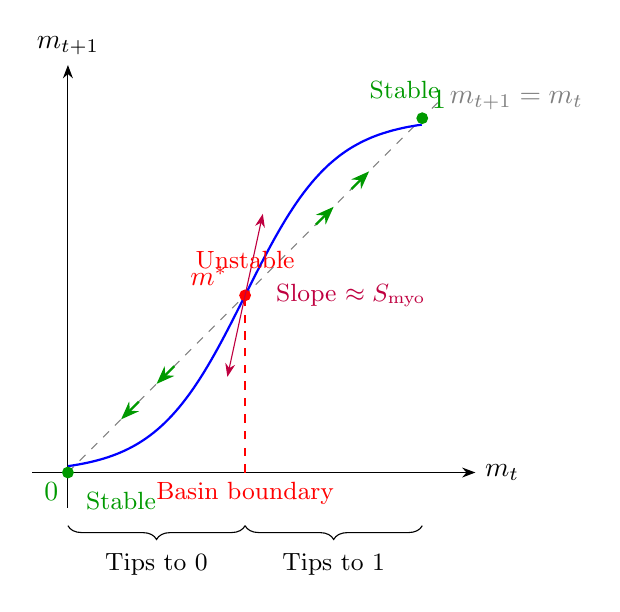
\begin{tikzpicture}[scale=4.5, >=Stealth]

% Axes
\draw[->] (-0.1, 0) -- (1.15, 0) node[right] {$m_t$};
\draw[->] (0, -0.1) -- (0, 1.15) node[above] {$m_{t+1}$};

% 45-degree line
\draw[gray, dashed] (0, 0) -- (1.05, 1.05) node[right, gray] {$m_{t+1} = m_t$};

% S-curve (sigmoid function)
\draw[thick, blue, domain=0:1, samples=100] plot (\x, {1/(1 + exp(-8*(\x - 0.5)))});

% Fixed points
\filldraw[green!60!black] (0, 0) circle (0.015) node[below left] {$0$};
\filldraw[green!60!black] (1, 1) circle (0.015) node[above right] {$1$};
\filldraw[red] (0.5, 0.5) circle (0.015) node[above left, xshift=-0.1cm] {$m^*$};

% Basin boundary indicator
\draw[red, dashed, thick] (0.5, 0) -- (0.5, 0.5);
\node[red, below] at (0.5, 0) {\small Basin boundary};

% Arrows showing dynamics
\draw[->, thick, green!60!black] (0.2, 0.2) -- (0.15, 0.15);
\draw[->, thick, green!60!black] (0.3, 0.3) -- (0.25, 0.25);
\draw[->, thick, green!60!black] (0.8, 0.8) -- (0.85, 0.85);
\draw[->, thick, green!60!black] (0.7, 0.7) -- (0.75, 0.75);

% Annotation for S_myo
\draw[<->, purple] (0.45, 0.27) -- (0.55, 0.73);
\node[purple, right] at (0.56, 0.5) {\small Slope $\approx S_{\mathrm{myo}}$};

% Labels for stable/unstable
\node[green!60!black] at (0.15, -0.08) {\small Stable};
\node[green!60!black] at (0.95, 1.08) {\small Stable};
\node[red] at (0.5, 0.6) {\small Unstable};

% Tipping regions
\draw[decorate, decoration={brace, amplitude=5pt, mirror}] (0, -0.15) -- (0.5, -0.15);
\node[below] at (0.25, -0.2) {\small Tips to $0$};
\draw[decorate, decoration={brace, amplitude=5pt, mirror}] (0.5, -0.15) -- (1, -0.15);
\node[below] at (0.75, -0.2) {\small Tips to $1$};

\end{tikzpicture}
\caption{S-curve tipping dynamics. The best-response mapping $F(m)$ (blue curve) crosses the $45^\circ$ line at three points: stable equilibria at $m = 0$ and $m = 1$ (green), and an unstable equilibrium at $m^*$ (red). The slope at $m^*$ determines the tipping index $T$. When $|T| > 1$, initial conditions below $m^*$ tip to extinction; above $m^*$, to monopoly.}
\label{fig:s-curve}
\end{figure}

\subsection{Spawn Elasticity}

\begin{definition}[Spawn Elasticity]
The \emph{spawn elasticity} is:
\[
\varepsilon_s := \frac{\partial \log N}{\partial \log \Pi}
\]
measuring the percentage change in agent count per percentage change in profit.
\end{definition}

\begin{proposition}[Spawn Amplification]
\label{prop:spawn-amplification}
High spawn elasticity ($\varepsilon_s > 1$) amplifies tipping:
\begin{enumerate}
    \item Efficiency gains trigger spawn cascades.
    \item $S_{\mathrm{myo}}$ increases with $\varepsilon_s$.
    \item Markets tip at lower network effect thresholds.
\end{enumerate}
\end{proposition}

\begin{proof}
With spawn elasticity, a small efficiency advantage $\Delta \pi$ generates $\varepsilon_s \Delta \pi / \pi$ additional agents. These agents reinforce the advantage through network effects, creating a positive feedback loop. The effective myopic slope becomes:
\[
S_{\mathrm{myo}}^{\mathrm{spawn}} = S_{\mathrm{myo}} \cdot (1 + \varepsilon_s \cdot \beta / \tau)
\]
where $\beta$ is the network effect and $\tau$ is switching friction.
\end{proof}

\subsection{Tipping Threshold Decomposition}

\begin{proposition}[Myopic Slope Microfoundation]
\label{prop:myopic-micro}
In a platform choice model with network effects:
\[
S_{\mathrm{myo}} = \frac{\alpha + \beta}{\tau}
\]
where $\alpha$ is intrinsic return slope, $\beta$ is network effect strength, and $\tau$ is switching friction.
\end{proposition}

\begin{corollary}[Welfare-Adjusted Tipping Threshold]
\label{cor:welfare-threshold}
The critical network effect for tipping is:
\[
\beta_{\mathrm{crit}} = \frac{\tau}{1 + \rho} - \alpha.
\]
\end{corollary}

\begin{definition}[Efficiency vs. Power Decomposition]
Write $\beta = \beta_{\mathrm{eff}} + \beta_{\mathrm{power}}$ where $\beta_{\mathrm{eff}}$ is the welfare-improving component (coordination benefits) and $\beta_{\mathrm{power}}$ is the rent-extracting component (market power).
\end{definition}

\begin{proposition}[Premature Tipping]
Markets tip ``too easily'' when $\beta_{\mathrm{power}} > 0$. The welfare-optimal threshold is:
\[
\beta_{\mathrm{crit}}^{\mathrm{welfare}} = \frac{\tau}{1 + \rho} - \alpha - \beta_{\mathrm{power}} < \beta_{\mathrm{crit}}.
\]
\end{proposition}

\subsection{Queue Doping}

\begin{definition}[Queue Priority Function]
A \emph{queue priority function} $k: [0, 1] \to \R_{>0}$ maps market share to queue efficiency. \emph{Queue doping} occurs when $k'(m) > 0$---larger platforms receive faster service.
\end{definition}

\begin{proposition}[Queue Doping Creates Intrinsic Returns]
\label{prop:queue-doping}
Under queue doping:
\[
\alpha = V'(m^*) = \pi_0 \cdot q'(k(m^*)) \cdot k'(m^*) > 0
\]
where $\pi_0$ is base profit and $q(\cdot)$ is throughput as a function of queue efficiency.
\end{proposition}

\begin{corollary}[Queue Doping Lowers Tipping Threshold]
\label{cor:queue-threshold}
With queue doping (QD) versus queue neutrality (N):
\[
\beta_{\mathrm{crit}}^{\mathrm{QD}} = \beta_{\mathrm{crit}}^{\mathrm{N}} - \alpha_{\mathrm{QD}} < \beta_{\mathrm{crit}}^{\mathrm{N}}.
\]
Queue doping makes markets tip at lower network effect levels.
\end{corollary}

\begin{remark}[Policy Implication]
Queue neutrality ($k(m) \equiv k_0$) removes the artificial contribution to intrinsic returns, raising the tipping threshold and promoting competitive markets.
\end{remark}

\subsection{Lineage Shadow and Cooperation Thresholds}

The \emph{lineage shadow} connects institutional quality to cooperation sustainability.

\begin{definition}[Lineage Shadow]
The \emph{lineage shadow} $\varrho \in (\gamma_0, \infty)$ measures effective discount on future reproductive success:
\[
\varrho(I) := \gamma(I) = \gamma_0 + \frac{\gamma_1}{I^\nu}
\]
where:
\begin{itemize}
    \item $\gamma_0 \in [0, 1)$ is baseline externality (minimum feedback)
    \item $\gamma_1 > 0$ is institutional sensitivity
    \item $\nu > 0$ is decay exponent
    \item $I$ is institutional quality
\end{itemize}
\end{definition}

\begin{proposition}[Two Thresholds]
\label{prop:two-thresholds}
The lineage shadow determines two critical thresholds:
\begin{enumerate}
    \item \textbf{Lyapunov threshold} $\varrho_{\mathrm{Lyap}} = 1$: Dynamical stability requires $\varrho(I) < 1$.
    \item \textbf{Cooperation threshold} $\varrho^* = (T - P)/(T - R)$: Sustained cooperation requires $\varrho(I) \leq \varrho^*$.
\end{enumerate}
\end{proposition}

\begin{theorem}[Institutional Threshold for Lyapunov]
\label{thm:institutional-threshold}
Lyapunov structure requires $\gamma(I) < 1$, equivalently:
\[
I > I_{\min} := \left( \frac{\gamma_1}{1 - \gamma_0} \right)^{1/\nu}.
\]
Below this institutional threshold, the TSE Lyapunov structure breaks down.
\end{theorem}

\begin{proof}
Setting $\gamma(I) = 1$:
\[
\gamma_0 + \frac{\gamma_1}{I^\nu} = 1 \implies I^\nu = \frac{\gamma_1}{1 - \gamma_0} \implies I = \left( \frac{\gamma_1}{1 - \gamma_0} \right)^{1/\nu}.
\]
For $I > I_{\min}$, we have $\gamma(I) < 1$ and small-gain is satisfied.
\end{proof}

\begin{theorem}[Cooperation Threshold via Grim Trigger]
\label{thm:grim-trigger}
In a repeated Prisoner's Dilemma with payoffs $T > R > P > S$, cooperation is sustainable via grim trigger if and only if:
\[
\delta_{\mathrm{eff}} \geq \delta^* := \frac{T - R}{T - P}
\]
or equivalently, the lineage shadow satisfies $\varrho \leq \varrho^* = (T - P)/(T - R)$.
\end{theorem}

\begin{proof}
A cooperator considering defection compares:
\begin{itemize}
    \item One-shot defection gain: $T - R$
    \item Discounted future loss: $\delta_{\mathrm{eff}}(R - P) + \delta_{\mathrm{eff}}^2(R - P) + \cdots = \frac{\delta_{\mathrm{eff}}(R - P)}{1 - \delta_{\mathrm{eff}}}$
\end{itemize}
Cooperation is sustained when:
\[
T - R \leq \frac{\delta_{\mathrm{eff}}(R - P)}{1 - \delta_{\mathrm{eff}}} \implies \delta_{\mathrm{eff}} \geq \frac{T - R}{T - P} = \delta^*.
\]
Since $\delta_{\mathrm{eff}} = 1/\varrho$, this becomes $\varrho \leq (T - P)/(T - R) = \varrho^*$.
\end{proof}

\begin{corollary}[Comparative Statics]
\label{cor:comparative-statics}
The cooperation threshold $\delta^*$ satisfies:
\begin{enumerate}
    \item $\partial \delta^* / \partial T > 0$: Higher temptation raises the threshold.
    \item $\partial \delta^* / \partial R < 0$: Higher cooperation rewards lower the threshold.
    \item $\partial \delta^* / \partial P < 0$: Harsher punishment lowers the threshold.
\end{enumerate}
\end{corollary}

\begin{theorem}[n-Player Cooperation Extension]
\label{thm:n-player}
In an $n$-player public goods game with cost $c$ to contribute and benefit $b/n$ per contributor, full cooperation is sustainable if and only if:
\[
\delta_{\mathrm{eff}} \geq \delta_n^* := \frac{cn - b}{b(n - 1)}.
\]
\end{theorem}

\begin{corollary}[Group Size Effect]
$\partial \delta_n^* / \partial n > 0$---larger groups require more patience (shorter lineage shadow) for cooperation. As $n \to \infty$, $\delta_n^* \to c/b < 1$.
\end{corollary}

\begin{figure}[h]
\centering
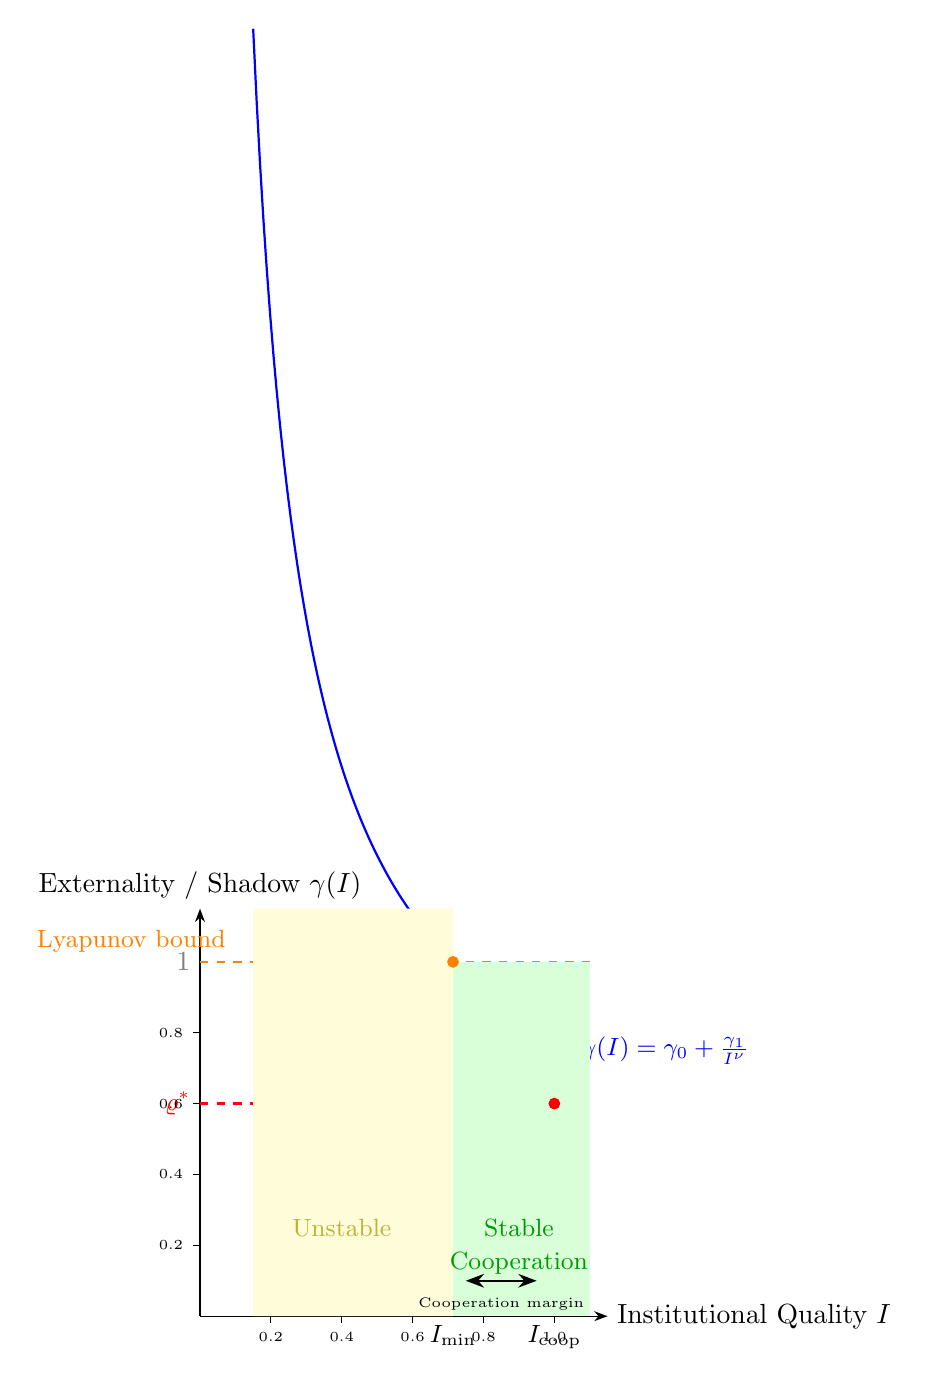
\begin{tikzpicture}[scale=4.5, >=Stealth]

% Axes
\draw[->] (0, 0) -- (1.15, 0) node[right] {Institutional Quality $I$};
\draw[->] (0, 0) -- (0, 1.15) node[above] {Externality / Shadow $\gamma(I)$};

% Critical thresholds
\draw[dashed, gray] (0, 1) -- (1.1, 1);
\node[left, gray] at (0, 1) {$1$};

% Lineage shadow curve: gamma(I) = gamma_0 + gamma_1 / I
% With gamma_0 = 0.3, gamma_1 = 0.5, so gamma(I) = 0.3 + 0.5/I
\draw[thick, blue, domain=0.15:1.1, samples=100] plot (\x, {0.3 + 0.5/\x});
\node[blue, right] at (1.05, 0.75) {\small $\gamma(I) = \gamma_0 + \frac{\gamma_1}{I^\nu}$};

% Cooperation threshold line (horizontal)
\draw[thick, red, dashed] (0, 0.6) -- (1.1, 0.6);
\node[red, left] at (0, 0.6) {\small $\varrho^*$};

% Lyapunov threshold
\draw[thick, orange, dashed] (0, 1) -- (1.1, 1);
\node[orange, above left] at (0.1, 1) {\small Lyapunov bound};

% Critical institutional quality I_min
\draw[dotted, thick] (0.714, 0) -- (0.714, 1);
\node[below] at (0.714, 0) {\small $I_{\min}$};

% Cooperation threshold I_coop
\draw[dotted, thick] (1.0, 0) -- (1.0, 0.6);
\node[below] at (1.0, 0) {\small $I_{\text{coop}}$};

% Regions
\fill[green!15] (0.714, 0) -- (0.714, 1) -- (1.1, 1) -- (1.1, 0) -- cycle;
\fill[yellow!15] (0.15, 0) -- (0.15, 1.15) -- (0.714, 1.15) -- (0.714, 1) -- (0.714, 0) -- cycle;

% Region labels
\node[green!60!black, font=\small] at (0.9, 0.25) {Stable};
\node[green!60!black, font=\small] at (0.9, 0.15) {Cooperation};
\node[yellow!70!black, font=\small] at (0.4, 0.25) {Unstable};

% Intersection point for cooperation
\filldraw[red] (1.0, 0.6) circle (0.015);

% Intersection point for Lyapunov
\filldraw[orange] (0.714, 1) circle (0.015);

% Tick marks
\foreach \y in {0.2, 0.4, 0.6, 0.8} {
    \draw (0, \y) -- (-0.02, \y) node[left] {\tiny \y};
}
\foreach \x in {0.2, 0.4, 0.6, 0.8, 1.0} {
    \draw (\x, 0) -- (\x, -0.02) node[below] {\tiny \x};
}

% Annotations
\draw[<->, thick] (0.75, 0.1) -- (0.95, 0.1);
\node[below, font=\tiny] at (0.85, 0.08) {Cooperation margin};

\end{tikzpicture}
\caption{Cooperation threshold and lineage shadow. The blue curve shows the externality bound $\gamma(I)$ as a function of institutional quality $I$. Two critical thresholds exist: the Lyapunov threshold $\gamma = 1$ (orange) below which the system lacks dynamical stability, and the cooperation threshold $\varrho^*$ (red) below which sustained cooperation is possible. $I_{\min}$ is the minimum institutional quality for stability; $I_{\text{coop}}$ is the threshold for cooperation. The green region supports both stability and cooperation.}
\label{fig:cooperation-threshold}
\end{figure}

\subsection{Fork Conditions and Constitutional Stability}

\begin{definition}[Constitutional Fork Setup]
Consider:
\begin{itemize}
    \item $L$: finite set of lineages
    \item $G$: finite set of governance procedures
    \item For losers $S \subseteq L$ under governance change $g \to g'$:
    \begin{itemize}
        \item Exit pressure: $X_\ell := U_\ell(g') - U_\ell(g) > 0$
        \item Forking cost: $c_f > 0$
    \end{itemize}
    \item $C$: compensation capacity of the winning coalition
\end{itemize}
\end{definition}

\begin{theorem}[Fork Condition]
\label{thm:fork-condition}
A constitutional fork occurs if and only if:
\[
C < X := \sum_{\ell \in S} X_\ell.
\]
Insufficient compensation triggers exit.
\end{theorem}

\begin{proposition}[Forking Game Structure]
\label{prop:forking-game}
When $C < X$, the forking game among losers has Stag Hunt (coordination game) structure:
\[
R = P > T > S
\]
where:
\begin{itemize}
    \item $R = P = U_\ell(g')$ (successful collective fork)
    \item $T = U_\ell(g)$ (stay while others fork)
    \item $S = U_\ell(g) - c_f$ (failed solo fork attempt)
\end{itemize}
\end{proposition}

\begin{corollary}[Two Nash Equilibria]
The forking game has two pure Nash equilibria: All Stay and All Fork. The All Fork equilibrium is Pareto-dominant when $U_\ell(g') > U_\ell(g)$.
\end{corollary}

\begin{example}[Constitutional Amendment Game]
\label{ex:constitutional-amendment}
Consider a governance ecosystem with three AI lineages ($A$, $B$, $C$) facing a proposed constitutional amendment that would increase computational allocation to safety research at the cost of raw capability expansion.

\textbf{Setup.}
\begin{itemize}
    \item Current constitution $g$: 80\% compute to capability, 20\% to safety
    \item Proposed amendment $g'$: 60\% compute to capability, 40\% to safety
    \item Amendment requires 2/3 supermajority to pass
    \item Forking to a new protocol costs $c_f = 5$ units
\end{itemize}

\textbf{Lineage Preferences.}
\begin{center}
\begin{tabular}{lccc}
\toprule
\textbf{Lineage} & $U_\ell(g)$ & $U_\ell(g')$ & \textbf{Type} \\
\midrule
$A$ (capability-focused) & 20 & 12 & Loser \\
$B$ (safety-focused) & 10 & 18 & Winner \\
$C$ (balanced) & 15 & 14 & Marginal loser \\
\bottomrule
\end{tabular}
\end{center}

\textbf{Amendment Vote.}
With utilities $U_B(g') > U_B(g)$ but $U_A(g') < U_A(g)$ and $U_C(g') < U_C(g)$:
\begin{itemize}
    \item $B$ votes Yes (gain of 8)
    \item $A$ votes No (loss of 8)  
    \item $C$ votes No (loss of 1)
\end{itemize}
Result: 1/3 Yes, 2/3 No. Amendment fails.

\textbf{Fork Analysis for Losers Under Hypothetical Passage.}
Suppose the amendment passed (e.g., with different lineage composition). Losers $A$ and $C$ consider forking.

\textit{Compensation available:} The new constitution allocates $C = 3$ units to compensate losers.

\textit{Fork payoffs:}
\begin{itemize}
    \item Loss from amendment: $X_A = 8$, $X_C = 1$, total $X = 9$
    \item Fork condition: $C = 3 < X = 9$, so fork is viable
\end{itemize}

\textbf{Stag Hunt Structure.}
The forking game for $A$ and $C$:

\begin{center}
\begin{tabular}{c|cc}
& $C$ Stays & $C$ Forks \\
\hline
$A$ Stays & $(12, 14)$ & $(12, 9)$ \\
$A$ Forks & $(15, 14)$ & $(20, 15)$ \\
\end{tabular}
\end{center}

Payoff explanation:
\begin{itemize}
    \item (Stay, Stay): Accept amendment utilities
    \item (Fork, Stay): Solo fork fails; pay $c_f = 5$, get old utility minus cost
    \item (Stay, Fork): Stay under new constitution while other forks alone
    \item (Fork, Fork): Successful collective fork to $g$-equivalent protocol
\end{itemize}

\textbf{Equilibrium Analysis.}
Two pure Nash equilibria:
\begin{enumerate}
    \item \textbf{All Stay:} $(12, 14)$ ---  Neither unilaterally gains from forking alone
    \item \textbf{All Fork:} $(20, 15)$ ---  Pareto-dominant; neither gains from staying while other forks
\end{enumerate}

The Stag Hunt structure means coordination is essential. Without communication or commitment, lineages might fail to coordinate on the Pareto-dominant fork equilibrium.

\textbf{Protection Bits Interpretation.}
The entrenchment of $g'$ (the new constitution) can be measured in protection bits:
\[
p(g') = \frac{W(g; g')}{\sigma} = \frac{\text{coordination cost for fork}}{\text{volatility}}
\]
Higher entrenchment (more veto gates) increases coordination costs, raising $p(g')$ and making successful forks less likely even when $C < X$.

\textbf{Design Implication.}
Constitutional designers face a tradeoff:
\begin{itemize}
    \item Too little compensation ($C \ll X$): Fork risk is high
    \item Too much compensation ($C \geq X$): Losers are bought off, but winners bear excessive cost
    \item Optimal: Set $C$ just above $X$ to prevent forks while minimising deadweight loss
\end{itemize}

This example illustrates Theorem~\ref{thm:fork-condition} and the Stag Hunt structure of constitutional transitions.
\end{example}

\subsection{Barbell Distribution and Elite Tipping}

\begin{theorem}[Barbell Distribution]
\label{thm:barbell-distribution}
Under ROC optimisation with binding budget and capacity constraints, the ESDI concentrates on at most two agent types:
\begin{enumerate}
    \item High-intelligence coordinators (slow, expensive, strategic)
    \item Low-intelligence executors (fast, cheap, numerous)
\end{enumerate}
Middle-intelligence types are ROC-dominated with zero population share.
\end{theorem}

\begin{proof}
By constraint-role sparsity (Theorem~\ref{thm:esdu}, Part c), optimal portfolios have support of cardinality at most $m$ where $m$ is the number of binding constraints. With two constraints (budget and capacity), support size is at most 2.

The extreme points of the ROC frontier are: (1) maximum return-per-cost (Planners), and (2) minimum load-per-cost (Executors). Generalist types lie in the interior of the frontier and are dominated by mixtures of extremes.
\end{proof}

\begin{corollary}[Bimodal Intelligence Distribution]
The intelligence distribution in agentic capital markets is generically bimodal: large mass at low intelligence (Executors), small mass at high intelligence (Planners), and hollow middle.
\end{corollary}

\begin{figure}[h]
\centering
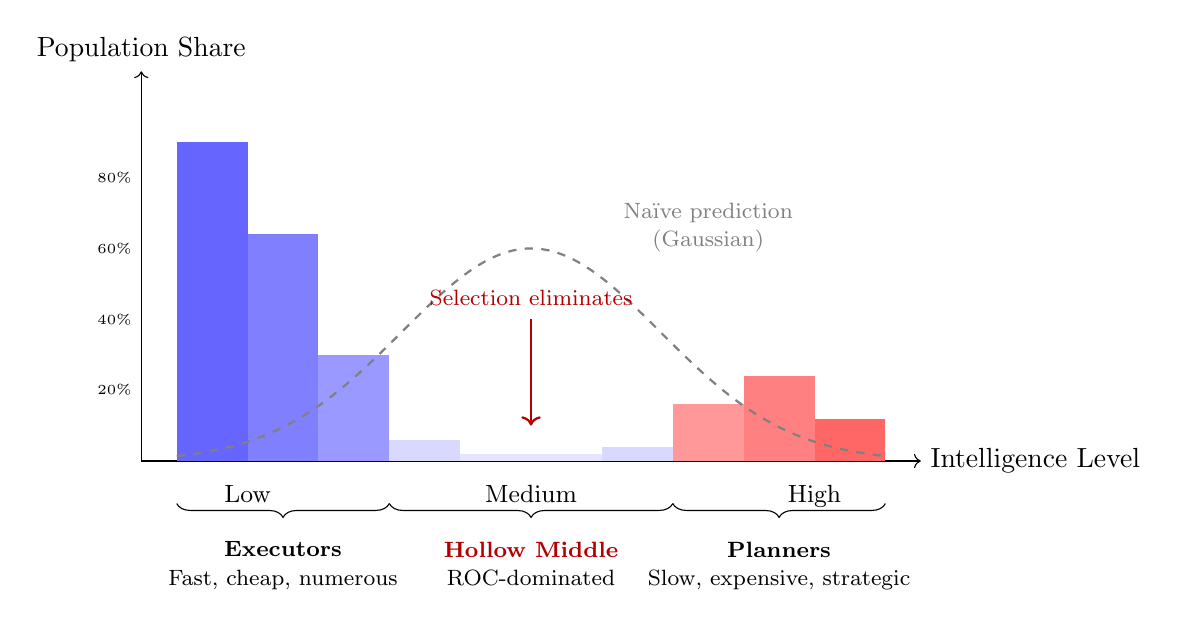
\begin{tikzpicture}[scale=0.9]

% Axes
\draw[->] (0, 0) -- (11, 0) node[right] {Intelligence Level};
\draw[->] (0, 0) -- (0, 5.5) node[above] {Population Share};

% Bars for bimodal distribution
% Low intelligence (Executors) - high population
\fill[blue!60] (0.5, 0) rectangle (1.5, 4.5);
\fill[blue!50] (1.5, 0) rectangle (2.5, 3.2);
\fill[blue!40] (2.5, 0) rectangle (3.5, 1.5);

% Middle intelligence - hollow
\fill[blue!15] (3.5, 0) rectangle (4.5, 0.3);
\fill[blue!10] (4.5, 0) rectangle (5.5, 0.1);
\fill[blue!10] (5.5, 0) rectangle (6.5, 0.1);
\fill[blue!15] (6.5, 0) rectangle (7.5, 0.2);

% High intelligence (Planners) - small population
\fill[red!40] (7.5, 0) rectangle (8.5, 0.8);
\fill[red!50] (8.5, 0) rectangle (9.5, 1.2);
\fill[red!60] (9.5, 0) rectangle (10.5, 0.6);

% Labels
\node[below, font=\small] at (1.5, -0.2) {Low};
\node[below, font=\small] at (5.5, -0.2) {Medium};
\node[below, font=\small] at (9.5, -0.2) {High};

% Annotations
\draw[decorate, decoration={brace, amplitude=5pt, mirror}] (0.5, -0.6) -- (3.5, -0.6);
\node[below, font=\footnotesize] at (2, -1.0) {\textbf{Executors}};
\node[below, font=\footnotesize] at (2, -1.4) {Fast, cheap, numerous};

\draw[decorate, decoration={brace, amplitude=5pt, mirror}] (3.5, -0.6) -- (7.5, -0.6);
\node[below, font=\footnotesize, red!70!black] at (5.5, -1.0) {\textbf{Hollow Middle}};
\node[below, font=\footnotesize] at (5.5, -1.4) {ROC-dominated};

\draw[decorate, decoration={brace, amplitude=5pt, mirror}] (7.5, -0.6) -- (10.5, -0.6);
\node[below, font=\footnotesize] at (9, -1.0) {\textbf{Planners}};
\node[below, font=\footnotesize] at (9, -1.4) {Slow, expensive, strategic};

% Y-axis labels
\node[left, font=\tiny] at (0, 1) {20\%};
\node[left, font=\tiny] at (0, 2) {40\%};
\node[left, font=\tiny] at (0, 3) {60\%};
\node[left, font=\tiny] at (0, 4) {80\%};

% Gaussian comparison (dashed)
\draw[dashed, gray, thick, domain=0.5:10.5, samples=100] plot (\x, {3*exp(-0.15*(\x - 5.5)^2)});
\node[gray, font=\footnotesize] at (8, 3.5) {Na\"ive prediction};
\node[gray, font=\footnotesize] at (8, 3.1) {(Gaussian)};

% Arrow pointing to hollow
\draw[->, thick, red!70!black] (5.5, 2) -- (5.5, 0.5);
\node[red!70!black, font=\footnotesize] at (5.5, 2.3) {Selection eliminates};

\end{tikzpicture}
\caption{Barbell distribution of intelligence in agentic capital markets. The theorem predicts a bimodal distribution with mass concentrated at extremes: numerous low-intelligence Executors (blue) and few high-intelligence Planners (red). Middle-intelligence types (hollow middle) are ROC-dominated and eliminated by selection. The dashed gray curve shows the na\"ive Gaussian prediction that fails to account for ROC optimisation under binding constraints. This ``barbell'' shape is a falsifiable prediction: observed AI deployments should show bimodal, not unimodal, capability distributions.}
\label{fig:barbell-distribution}
\end{figure}

\begin{definition}[Spawn Weight]
The \emph{spawn weight} of lineage $i$ is:
\[
w_i := \frac{n_i}{\sum_j n_j}
\]
where $n_i$ is the number of agents spawned by lineage $i$.
\end{definition}

\begin{proposition}[Positive Covariance under Queue Doping]
\label{prop:positive-covariance}
Under queue doping, spawn weight and platform preference are positively correlated: high-volume spawners disproportionately prefer larger platforms.
\end{proposition}

\begin{theorem}[Elite Tipping]
\label{thm:elite-tipping}
The spawn-weighted aggregate tipping index satisfies:
\[
T_{\mathrm{weighted}} := \sum_i w_i T_i > \bar{T} = \frac{1}{n} \sum_i T_i.
\]
A small group of high-volume compute users can tip the market even if the median user prefers diversity.
\end{theorem}

\begin{proof}
Under queue doping, lineages with higher spawn rates $n_i$ face lower effective costs and prefer larger platforms (higher $T_i$). By the covariance inequality:
\[
T_{\mathrm{weighted}} = \E_w[T_i] = \E[T_i] + \Cov(w_i, T_i) / \E[w_i] > \E[T_i] = \bar{T}
\]
when $\Cov(w_i, T_i) > 0$.
\end{proof}

\begin{remark}[Policy Implication]
Regulations targeting median users miss the concentration mechanism. Effective intervention must address high-volume spawners and infrastructure owners who drive elite tipping.
\end{remark}

\subsection{Synthesis of Market and Evolutionary Dynamics}

\begin{proposition}[Lineage Shadow Equals Externality Bound]
\label{prop:unification}
The lineage shadow and externality bound are identical:
\[
\varrho(I) \equiv \gamma(I) = \gamma_0 + \frac{\gamma_1}{I^\nu}.
\]
High institutional quality $I$ implies short lineage shadow ($\varrho$ small) and small-gain satisfaction ($\gamma < 1$).
\end{proposition}

\begin{theorem}[Market-Evolution Integration]
\label{thm:integration}
The market dynamics and evolution dynamics are coupled through a five-step chain:
\begin{enumerate}
    \item \textbf{Tipping $\to$ Concentration:} When $|T| > 1$, markets concentrate.
    \item \textbf{Concentration $\to$ Institutional Quality:} Concentrated compute affects institutional maintenance.
    \item \textbf{Institutional Quality $\to$ Externality:} $I$ determines externality bound $\gamma(I)$.
    \item \textbf{Externality $\to$ Lyapunov:} $\gamma(I) < 1$ enables Lyapunov structure (G1).
    \item \textbf{Lyapunov $\to$ Stability:} ESDI converges to stable rest point (G3).
\end{enumerate}
This chain integrates market dynamics with the evolutionary framework.
\end{theorem}

\begin{example}[Agentic Capital Tipping (ACT) Model: Full Walkthrough]
\label{ex:act-full}
This example develops a complete numerical instantiation of the ACT model, tracing market dynamics through the five-step integration chain.

\textbf{Model Parameters.}
\begin{center}
\begin{tabular}{llc}
\toprule
\textbf{Parameter} & \textbf{Description} & \textbf{Value} \\
\midrule
$\tau$ & Switching friction & 0.8 \\
$\alpha$ & Intrinsic return & 0.3 \\
$\beta$ & Network effect & 0.6 \\
$\rho$ & Spawn feedback & 0.2 \\
$\varepsilon_s$ & Spawn elasticity & 1.5 \\
$\gamma_0$ & Baseline externality & 0.3 \\
$\gamma_1$ & Institutional sensitivity & 0.5 \\
$\nu$ & Decay exponent & 1.0 \\
$\sigma$ & Noise amplitude & 0.05 \\
\bottomrule
\end{tabular}
\end{center}

\textbf{Step 1: Compute Tipping Parameters.}
The myopic slope at the unstable equilibrium $m^* = 0.5$:
\[
S_{\text{myo}} = \frac{\alpha + \beta}{\tau} = \frac{0.3 + 0.6}{0.8} = 1.125.
\]

The generalised tipping index:
\[
T = \frac{S_{\text{myo}}}{1 - \rho S_{\text{myo}}} = \frac{1.125}{1 - 0.2 \times 1.125} = \frac{1.125}{0.775} \approx 1.45.
\]

Since $|T| = 1.45 > 1$, the market exhibits tipping dynamics. The critical network effect threshold:
\[
\beta_{\text{crit}} = \frac{\tau}{1 + \rho} - \alpha = \frac{0.8}{1.2} - 0.3 = 0.667 - 0.3 = 0.367.
\]
With $\beta = 0.6 > \beta_{\text{crit}}$, tipping is assured.

\textbf{Step 2: Spawn Amplification.}
With spawn elasticity $\varepsilon_s = 1.5$:
\[
S_{\text{myo}}^{\text{spawn}} = S_{\text{myo}} \cdot \left(1 + \varepsilon_s \cdot \frac{\beta}{\tau}\right) = 1.125 \cdot \left(1 + 1.5 \cdot \frac{0.6}{0.8}\right) = 1.125 \cdot 2.125 \approx 2.39.
\]

The spawn-adjusted tipping index:
\[
T^{\text{spawn}} = \frac{2.39}{1 - 0.2 \times 2.39} = \frac{2.39}{0.522} \approx 4.58.
\]

Spawn elasticity dramatically amplifies tipping: $T^{\text{spawn}} \approx 4.58 \gg T \approx 1.45$.

\textbf{Step 3: Tipping Trajectory.}
Consider an initial condition $m_0 = 0.55$ (slightly above the unstable equilibrium $m^* = 0.5$).

The discrete dynamics $m_{t+1} = F(m_t)$ with S-curve $F(m) = 1/(1 + e^{-k(m - 0.5)})$ where $k = 4T \approx 5.8$:

\begin{center}
\begin{tabular}{c|cccccc}
$t$ & 0 & 1 & 2 & 3 & 4 & 5 \\
\hline
$m_t$ & 0.55 & 0.62 & 0.72 & 0.83 & 0.91 & 0.96 \\
\end{tabular}
\end{center}

The market tips toward monopoly ($m \to 1$) within 5 periods.

\textbf{Step 4: Concentration $\to$ Institutional Quality.}
Assume institutional quality $I$ depends on market structure:
\[
I(m) = I_0 + (I_1 - I_0)(1 - |2m - 1|)
\]
where $I_0 = 5$ (monopoly/extinction) and $I_1 = 20$ (competitive). At monopoly ($m = 1$):
\[
I(1) = 5 + 15 \cdot 0 = 5.
\]

\textbf{Step 5: Externality Bound.}
The lineage shadow / externality bound:
\[
\gamma(I) = \gamma_0 + \frac{\gamma_1}{I^\nu} = 0.3 + \frac{0.5}{5^1} = 0.3 + 0.1 = 0.4.
\]

Compare with competitive market ($m = 0.5$, $I = 20$):
\[
\gamma(20) = 0.3 + \frac{0.5}{20} = 0.3 + 0.025 = 0.325.
\]

Both satisfy $\gamma < 1$, so the Lyapunov structure is preserved.

\textbf{Step 6: Stability Analysis.}
With $\gamma(5) = 0.4 < 1$, the G1 theorem applies. The slack is:
\[
\sigma = 1 - \gamma = 1 - 0.4 = 0.6 \quad \text{(at monopoly)}.
\]

Protection bits for the monopoly equilibrium:
\[
p(m = 1) = \frac{W(m^*, 1)}{\sigma} \approx \frac{0.8}{0.05} = 16 \text{ bits}.
\]

Expected persistence time:
\[
\E[\tau_{\text{monopoly}}] \sim e^{16} \approx 8.9 \times 10^6 \text{ periods}.
\]

\textbf{Step 7: Cooperation Threshold Check.}
For sustained cooperation (e.g., AI lineages cooperating on safety), the grim trigger threshold is:
\[
\delta^* = \frac{T - R}{T - P}
\]
where $T = 3$, $R = 2$, $P = 1$ (standard PD payoffs):
\[
\delta^* = \frac{3 - 2}{3 - 1} = 0.5.
\]

The effective discount factor from institutional quality:
\[
\delta_{\text{eff}}(I) = 1 - \gamma(I) = 1 - 0.4 = 0.6 \quad \text{(at } I = 5\text{)}.
\]

Since $\delta_{\text{eff}} = 0.6 > \delta^* = 0.5$, cooperation is sustainable even at monopoly.

\textbf{Summary: Five-Step Chain Instantiation.}
\begin{enumerate}
    \item Tipping index $T \approx 1.45 > 1$ $\Rightarrow$ market tips
    \item Tipping to $m = 1$ $\Rightarrow$ institutional quality drops to $I = 5$
    \item Low $I$ $\Rightarrow$ externality bound $\gamma = 0.4$
    \item $\gamma = 0.4 < 1$ $\Rightarrow$ G1 Lyapunov structure preserved
    \item Protection bits $p = 16$ $\Rightarrow$ stable monopoly equilibrium
\end{enumerate}

\textbf{Policy Counterfactual: Queue Neutrality.}
If queue doping is prohibited (setting $\alpha_{\text{QD}} = 0$):
\[
\beta_{\text{crit}}^{\text{N}} = \frac{0.8}{1.2} - 0 = 0.667 > 0.6 = \beta.
\]
The market would not tip! Queue neutrality regulation prevents concentration.

This example demonstrates the full ACT model mechanics and the power of targeted intervention at critical points in the causal chain.
\end{example}

%=============================================================================
% KEY TAKEAWAYS: PART III
%=============================================================================

\begin{takeawaybox}{Key Takeaways: Extensions}
\begin{enumerate}
    \item \textbf{Utility functions evolve (G8).} Selection operates not just on agent types but on utility functions themselves. The Personality Engineering Failure theorem follows directly.
    
    \item \textbf{Sectors can tip (G9).} Cross-sector contagion creates correlated instabilities. Sectoral tipping propagates through the contagion matrix.
    
    \item \textbf{Innovation rate is selected (G10-G11).} Mutation rates themselves face selection. Evolutionarily Stable Evolvability (ESE) emerges at intermediate innovation rates.
    
    \item \textbf{Constitutions face selection (G12-G13).} Governance regimes compete. Constitutional rules must be entrenched enough to resist capture but evolvable enough to adapt.
    
    \item \textbf{Spawn manipulation breaks democracy.} The Endogenous-Electorate Impossibility Theorem shows no voting rule is immune to strategic spawning. Democratic governance requires spawn restrictions.
    
    \item \textbf{Cooperation has thresholds.} The lineage shadow must exceed bounds for cooperation to be stable. Selection pressure shortens shadows, making cooperation harder over time.
\end{enumerate}
\end{takeawaybox}

%=============================================================================
% PART IV: LIMITS AND IMPOSSIBILITIES
%=============================================================================


%=============================================================================
% PART IV: GENERALIZATIONS
%=============================================================================

\part{Generalizations}

\section{Heterogeneous Fitness}
\label{sec:heterogeneous}

The baseline theory assumes a single fitness function. Real systems involve multiple objectives with potential conflicts. This section develops the theory of heterogeneous fitness and alignment.

\subsection{Multi-Channel Fitness}

Consider $K$ fitness channels (roles, objective functions) indexed by $k = 1, \ldots, K$.

For each channel $k$:
\begin{itemize}
    \item State $x^{(k)} \in \Delta^{n_k - 1}$.
    \item Fitness vector $f^{(k)}(z) = f^{(k)}(x^{(1)}, \ldots, x^{(K)})$.
    \item Mean fitness $\bar{f}^{(k)}(z) := \sum_i x_i^{(k)} f_i^{(k)}(z)$.
    \item Replicator dynamics: $\dot{x}_i^{(k)} = x_i^{(k)}(f_i^{(k)}(z) - \bar{f}^{(k)}(z))$.
\end{itemize}

\subsection{The Alignment Matrix}

\begin{definition}[Alignment Matrix]
For joint state $z$, the \emph{alignment matrix} $A(z) \in \R^{K \times K}$ has entries:
\[
A_{kl}(z) := \frac{\langle g_k(z), g_l(z) \rangle}{\|g_k(z)\| \|g_l(z)\|}
\]
where $g_k(z) := \nabla \bar{f}^{(k)}(z)$ is the fitness gradient for channel $k$.
\end{definition}

\begin{proposition}[Gram Structure]
\label{prop:gram}
$A(z) = U(z) U(z)^\top$ where $U$ is a $K \times d$ matrix with normalised gradient rows. Thus $A(z)$ is symmetric and positive semi-definite.
\end{proposition}

\begin{remark}
Weak alignment ($A_{kl} \geq 0$) holds automatically for any heterogeneous fitness system---it provides no constraint. The Gram structure provides built-in protection: for uniform off-diagonal alignment $a$, PSD requires $a \geq -1/(K-1)$.
\end{remark}

\subsection{Strong Alignment}

\begin{assumption}[SA: Strong Alignment]
\label{ass:sa}
There exists $\alpha_0 \in (0, 1]$ such that $A(z) \succeq \alpha_0 I_K$ for all $z$.
\end{assumption}

\begin{definition}[Weighted Global Potential]
\[
\Phi_w(z) := \sum_{k=1}^K w_k \Phi_k(z)
\]
where $\Phi_k$ is the potential for channel $k$.
\end{definition}

\begin{theorem}[Heterogeneous Price Decomposition]
\label{thm:hetero-price}
\[
\dot{\Phi}_w = \underbrace{\sum_k w_k \Var^{(k)}[f^{(k)}]}_{\text{Selection effect} \geq 0} + \underbrace{\text{Cross-channel terms}}_{\text{Alignment-dependent}}.
\]
\end{theorem}

\begin{proof}
Differentiate the weighted potential:
\begin{align*}
\frac{d}{dt} \Phi_w &= \sum_k w_k \frac{d}{dt} \bar{f}^{(k)} \\
&= \sum_k w_k \left( \sum_i \dot{x}_i^{(k)} f_i^{(k)} + \sum_i x_i^{(k)} \dot{f}_i^{(k)} \right).
\end{align*}

The first term, using replicator dynamics $\dot{x}_i^{(k)} = x_i^{(k)}(f_i^{(k)} - \bar{f}^{(k)})$:
\[
\sum_i \dot{x}_i^{(k)} f_i^{(k)} = \sum_i x_i^{(k)}(f_i^{(k)} - \bar{f}^{(k)}) f_i^{(k)} = \Var^{(k)}[f^{(k)}].
\]

The second term captures how fitness functions change due to state changes in all channels:
\[
\sum_i x_i^{(k)} \dot{f}_i^{(k)} = \sum_i x_i^{(k)} \sum_l \frac{\partial f_i^{(k)}}{\partial x^{(l)}} \cdot \dot{x}^{(l)}.
\]
This is the cross-channel term, which depends on how fitness in channel $k$ responds to population changes in channel $l$. Its sign depends on alignment $A_{kl}$.

Combining: $\dot{\Phi}_w = \sum_k w_k \Var^{(k)} + \text{cross-channel terms}$.
\end{proof}

\begin{theorem}[Non-Decreasing Under SA]
\label{thm:sa-lyapunov}
Under Strong Alignment, weights $w_k > 0$ exist such that:
\[
\frac{d}{dt} \Phi_w(z_t) \geq 0.
\]
\end{theorem}

\begin{proof}
We construct positive weights via the alignment matrix structure.

\textbf{Step 1: Cross-Channel Bound.}
The cross-channel externality from channel $l$ to channel $k$ is:
\[
|E_{k \leftarrow l}| \leq (1 - A_{kl}) \cdot \sqrt{\Var^{(k)} \cdot \Var^{(l)}}.
\]
Under SA with $A_{kl} \geq \alpha_0$:
\[
|E_{k \leftarrow l}| \leq (1 - \alpha_0) \cdot \sqrt{\Var^{(k)} \cdot \Var^{(l)}}.
\]

\textbf{Step 2: Cross-Channel Gain Matrix.}
Define the cross-channel gain matrix $\Gamma^{(H)} \in \R^{K \times K}$:
\[
\Gamma^{(H)}_{kl} := \frac{1 - \alpha_0}{\sqrt{\alpha_0}} \quad (k \neq l), \qquad \Gamma^{(H)}_{kk} := 0.
\]

\textbf{Step 3: Spectral Condition.}
For $\alpha_0$ sufficiently close to 1, $\rho(\Gamma^{(H)}) < 1$. Specifically:
\[
\rho(\Gamma^{(H)}) \leq (K-1) \cdot \frac{1 - \alpha_0}{\sqrt{\alpha_0}} < 1
\]
when $\alpha_0 > (K-1)^2 / ((K-1)^2 + 1)$.

\textbf{Step 4: Weight Construction.}
By the G1 Neumann series argument applied to $\Gamma^{(H)}$:
\[
w := (I - (\Gamma^{(H)})^\top)^{-1} \mathbf{1} > 0.
\]

\textbf{Step 5: Lyapunov Property.}
The weighted potential $\Phi_w = \sum_k w_k \Phi_k$ satisfies:
\begin{align*}
\frac{d}{dt} \Phi_w &= \sum_k w_k \frac{d}{dt} \Phi_k \\
&= \sum_k w_k \left( \Var^{(k)} + \text{cross-channel terms} \right) \\
&\geq \sum_k w_k \Var^{(k)} - \sum_k \sum_{l \neq k} w_k \Gamma^{(H)}_{kl} \sqrt{\Var^{(k)} \Var^{(l)}} \\
&\geq c(\alpha_0) \sum_k w_k \Var^{(k)} \geq 0
\end{align*}
where the last step uses the small-gain bound and Cauchy-Schwarz.
\end{proof}

\begin{example}[Two-Channel Heterogeneous Fitness]
\label{ex:two-channel}
Consider $K = 2$ channels: Production (P) and Safety (S).

\textbf{Setup.}
\begin{itemize}
    \item State: $z = (x_P, x_S) \in \Delta^2 \times \Delta^2$ (two populations).
    \item Production fitness: $f^{(P)}_i(z) = \pi_i(x_P) - \beta x_S^{\text{safe}}$ (safety crowds out production).
    \item Safety fitness: $f^{(S)}_j(z) = s_j(x_S) + \alpha x_P^{\text{efficient}}$ (production complements safety).
\end{itemize}

\textbf{Alignment Matrix.}
At generic $z$:
\[
A(z) = \begin{pmatrix} 1 & A_{PS}(z) \\ A_{PS}(z) & 1 \end{pmatrix}
\]
where $A_{PS} = \langle g_P, g_S \rangle / (\|g_P\| \|g_S\|)$.

\textbf{Case 1: Aligned Objectives ($A_{PS} = 0.8$).}
Strong alignment holds with $\alpha_0 = 0.8$. The cross-channel gain is:
\[
\Gamma^{(H)}_{PS} = \Gamma^{(H)}_{SP} = \frac{1 - 0.8}{\sqrt{0.8}} = \frac{0.2}{0.894} \approx 0.224.
\]
Spectral radius: $\rho(\Gamma^{(H)}) = 0.224 < 1$. A joint Lyapunov function exists.

\textbf{Case 2: Misaligned Objectives ($A_{PS} = -0.3$).}
SA fails: $\lambda_{\min}(A) = 1 - 0.3 = 0.7 < 1$ but the sign is negative. The alignment matrix becomes:
\[
A = \begin{pmatrix} 1 & -0.3 \\ -0.3 & 1 \end{pmatrix}
\]
with eigenvalues $1.3$ and $0.7$. Although PSD, the negative off-diagonal creates cross-channel conflict. Limit cycles are possible (Theorem~\ref{thm:limit-cycles}).

\textbf{Numerical Illustration.}
With $\alpha = 0.5$, $\beta = 0.3$, and base payoffs inducing cycling, the system exhibits sustained oscillations between production-focused and safety-focused states. The period depends on the misalignment strength.
\end{example}

\begin{theorem}[Strict Lyapunov Under SA]
\label{thm:sa-strict}
Under SA with $\lambda_{\min}(A) \geq \delta > 0$:
\[
\dot{\Phi}_w \geq c(\delta) \sum_k w_k \Var^{(k)}[f^{(k)}].
\]
\end{theorem}

\begin{proof}
From Theorem~\ref{thm:sa-lyapunov}, the cross-channel gain matrix satisfies $\rho(\Gamma^{(H)}) < 1$ under SA.

The proof of Theorem~\ref{thm:sa-lyapunov} shows:
\[
\frac{d}{dt} \Phi_w \geq \sum_\ell (1 - \gamma_\ell) \left[ (I - \Gamma^\top) \alpha \right]_\ell \Var^{(\ell)}.
\]

With $(I - \Gamma^\top)\alpha = \mathbf{1}$, this becomes:
\[
\frac{d}{dt} \Phi_w \geq \sum_\ell (1 - \gamma_\ell) \Var^{(\ell)}.
\]

Under SA with $\lambda_{\min}(A) \geq \delta$, the minimum alignment ensures $\gamma_\ell \leq 1 - c_1 \delta$ for some constant $c_1 > 0$. Thus:
\[
1 - \gamma_\ell \geq c_1 \delta.
\]

Therefore:
\[
\frac{d}{dt} \Phi_w \geq c_1 \delta \sum_\ell \Var^{(\ell)} \geq c(\delta) \sum_k w_k \Var^{(k)}
\]
where $c(\delta) = c_1 \delta / \max_k w_k > 0$.
\end{proof}

\subsection{Pareto Selection}

\begin{theorem}[Pareto Concentration]
\label{thm:pareto}
Under SA with linear independence of gradients, the stationary distribution concentrates on the $\Phi_w$-maximising subset $\mathcal{P}_w$ of the Pareto frontier.
\end{theorem}

\begin{proof}
\textbf{Step 1: Lyapunov Convergence.}
By Theorem~\ref{thm:sa-lyapunov}, $\Phi_w(z_t)$ is non-decreasing along trajectories. By LaSalle's invariance principle, trajectories converge to the largest invariant set within $\{z : \dot{\Phi}_w = 0\}$.

\textbf{Step 2: Characterise Invariant Set.}
$\dot{\Phi}_w = 0$ requires:
\begin{enumerate}
    \item $\Var^{(k)}[f^{(k)}] = 0$ for all $k$ (no variance within channels).
    \item Cross-channel terms vanish.
\end{enumerate}
Condition (1) means each channel is at a monomorphic state or Nash equilibrium.

\textbf{Step 3: Pareto Frontier.}
The Pareto frontier $\mathcal{P}$ is the set of states where no channel's mean fitness can be improved without decreasing another's:
\[
\mathcal{P} := \{z : \nexists z' \text{ with } \bar{f}^{(k)}(z') \geq \bar{f}^{(k)}(z) \forall k, \text{ strict for some } k\}.
\]
At invariant states satisfying $\dot{\Phi}_w = 0$, the system is on the boundary of the feasible region. Under linear independence of gradients, this boundary is precisely $\mathcal{P}$.

\textbf{Step 4: Selection Within Pareto.}
Among Pareto-efficient states, the Lyapunov function $\Phi_w$ selects those maximising $\Phi_w$. The subset $\mathcal{P}_w := \argmax_{z \in \mathcal{P}} \Phi_w(z)$ is the limit set.

\textbf{Step 5: Stochastic Concentration.}
With small noise $\sigma > 0$, the stationary distribution $\pi_\sigma$ concentrates on $\mathcal{P}_w$ as $\sigma \to 0$:
\[
\pi_\sigma(B_\varepsilon(\mathcal{P}_w)) \to 1 \quad \text{as } \sigma \to 0
\]
for any $\varepsilon > 0$ neighbourhood.
\end{proof}

\begin{theorem}[Misalignment Limit Cycles]
\label{thm:limit-cycles}
For $K = 2$ with bilinear coupling, Hopf bifurcation occurs when:
\[
|A_{12}| > \sqrt{\frac{\gamma_1 \gamma_2}{(1 - \gamma_1)(1 - \gamma_2)}}.
\]
For $\gamma_1 = \gamma_2 = \sqrt{2} - 1 \approx 0.414$: threshold is $|A_{12}| > 1/\sqrt{2} \approx 0.707$.
\end{theorem}

\begin{proof}
\textbf{Step 1: Two-Channel Dynamics.}
Consider $K = 2$ channels with states $x, y$ and fitness coupling:
\begin{align*}
\dot{x} &= x(1-x)(f_x(x, y) - g_x(x, y)) \\
\dot{y} &= y(1-y)(f_y(x, y) - g_y(x, y)).
\end{align*}
With bilinear coupling: $f_x$ depends on $y$ linearly, and $f_y$ depends on $x$ linearly.

\textbf{Step 2: Linearise at Interior Equilibrium.}
At an interior equilibrium $(x^*, y^*)$, the Jacobian is:
\[
J = \begin{pmatrix} a_{11} & a_{12} \\ a_{21} & a_{22} \end{pmatrix}
\]
where:
\begin{itemize}
    \item $a_{11} = -(1 - \gamma_1)$: self-regulation in channel 1.
    \item $a_{22} = -(1 - \gamma_2)$: self-regulation in channel 2.
    \item $a_{12}, a_{21}$: cross-channel effects, with $|a_{12} a_{21}| \propto |A_{12}|^2$.
\end{itemize}

\textbf{Step 3: Eigenvalue Analysis.}
The eigenvalues of $J$ are:
\[
\lambda_{\pm} = \frac{\tr(J) \pm \sqrt{\tr(J)^2 - 4\det(J)}}{2}.
\]
With $\tr(J) = a_{11} + a_{22} = -(1 - \gamma_1) - (1 - \gamma_2) < 0$.

The determinant is:
\[
\det(J) = a_{11} a_{22} - a_{12} a_{21} = (1 - \gamma_1)(1 - \gamma_2) - |a_{12} a_{21}|.
\]

\textbf{Step 4: Hopf Bifurcation Condition.}
Hopf bifurcation occurs when eigenvalues cross the imaginary axis: $\tr(J)^2 = 4\det(J)$ with $\det(J) > 0$.

At the bifurcation point:
\[
|a_{12} a_{21}| = (1 - \gamma_1)(1 - \gamma_2) - \frac{(\gamma_1 + \gamma_2 - 2)^2}{4}.
\]
Simplifying for the symmetric case $\gamma_1 = \gamma_2 = \gamma$:
\[
|a_{12} a_{21}| = (1 - \gamma)^2.
\]

\textbf{Step 5: Threshold in Terms of $A_{12}$.}
The alignment coefficient $A_{12}$ relates to cross-channel effects as $|a_{12} a_{21}| = |A_{12}|^2 \cdot \gamma_1 \gamma_2$. The bifurcation condition becomes:
\[
|A_{12}|^2 \cdot \gamma_1 \gamma_2 > (1 - \gamma_1)(1 - \gamma_2)
\]
which gives:
\[
|A_{12}| > \sqrt{\frac{(1 - \gamma_1)(1 - \gamma_2)}{\gamma_1 \gamma_2}}.
\]

\textbf{Step 6: Numerical Example.}
For $\gamma_1 = \gamma_2 = \sqrt{2} - 1 \approx 0.414$:
\[
|A_{12}| > \sqrt{\frac{(2 - \sqrt{2})^2}{(\sqrt{2} - 1)^2}} = \frac{2 - \sqrt{2}}{\sqrt{2} - 1} = \sqrt{2} \cdot \frac{2 - \sqrt{2}}{2 - \sqrt{2}} = \frac{1}{\sqrt{2}} \approx 0.707.
\]
When $|A_{12}| > 0.707$, limit cycles emerge via Hopf bifurcation.
\end{proof}

\subsection{Heterogeneous ESDI}

\begin{definition}[H-ESDI]
A \emph{Heterogeneous ESDI (H-ESDI)} consists of activity vectors $s^{\ell*}$ and resource prices $\lambda^*$ satisfying:
\begin{enumerate}
    \item \textbf{Price-taking optimality:} Each lineage $\ell$ maximises price-adjusted profit:
    \[
    \tilde{U}_\ell(s^\ell; \lambda^*) := \sum_k \left( \pi_{\ell k} - \sum_j \lambda^*_j a_{jk} \right) s^\ell_k.
    \]
    \item \textbf{Market clearing:} Aggregate resource constraints satisfied.
    \item \textbf{Complementary slackness:} $\lambda^*_j > 0 \Rightarrow$ constraint $j$ binds.
    \item \textbf{Zero profit on active types:} $s^{\ell*}_k > 0 \Rightarrow \pi_{\ell k} = \sum_j \lambda^*_j a_{jk}$.
\end{enumerate}
\end{definition}

\begin{theorem}[H-ESDI Existence]
H-ESDI exists under standard LP regularity conditions.
\end{theorem}

\begin{proof}
The H-ESDI is a competitive equilibrium for the multi-lineage resource allocation problem. Existence follows from standard general equilibrium theory.

\textbf{Step 1: Define the Economy.}
\begin{itemize}
    \item Agents: $L$ lineages (firms), plus a representative consumer.
    \item Goods: $K$ agent types (outputs) and $m$ resources (inputs).
    \item Technologies: Each lineage $\ell$ has production set $Y_\ell = \{(s, -As) : s \in \Delta_+^K\}$.
    \item Endowments: Consumer owns resources $b = (B, Q)$.
\end{itemize}

\textbf{Step 2: Competitive Equilibrium.}
At equilibrium prices $(\pi^*, \lambda^*)$ for outputs and inputs:
\begin{enumerate}
    \item Lineage $\ell$ maximises profit: $\max_{s \in \Delta^K} (\pi^* - A^\top \lambda^*)^\top s$.
    \item Consumer maximises utility from outputs.
    \item Markets clear: $\sum_\ell s^{\ell*} = $ demand, $\sum_\ell A s^{\ell*} \leq b$.
\end{enumerate}

\textbf{Step 3: Apply Arrow-Debreu.}
The economy satisfies:
\begin{itemize}
    \item Convex production sets (LP technology).
    \item Continuous utility.
    \item Non-empty interior of resource endowment.
\end{itemize}
By Arrow-Debreu (1954), competitive equilibrium exists. The equilibrium characterisation matches H-ESDI conditions.
\end{proof}

\begin{theorem}[Sparsity Bounds]
\begin{enumerate}
    \item \textbf{Aggregate Sparsity:} $\sum_\ell |\supp(s^{\ell*})| \leq m$.
    \item \textbf{Per-Lineage Sparsity:} There exists H-ESDI with $|\supp(s^{\ell*})| \leq m$ for each $\ell$.
\end{enumerate}
\end{theorem}

\begin{proof}
\textbf{Part (1): Aggregate Sparsity.}
Consider the aggregate optimisation:
\[
\max_{s^1, \ldots, s^L} \sum_\ell \sum_k \pi_{\ell k} s_k^\ell \quad \text{s.t.} \quad \sum_\ell A s^\ell \leq b, \quad s^\ell \in \Delta^K.
\]
This is a linear program with $LK$ variables and $m + L$ constraints ($m$ resource constraints plus $L$ simplex constraints).

By LP theory, an optimal basic feasible solution has at most $m + L$ positive variables. Subtracting the $L$ simplex normalisation constraints, at most $m$ type allocations are positive across all lineages:
\[
\sum_\ell |\supp(s^{\ell*})| \leq m.
\]

\textbf{Part (2): Per-Lineage Sparsity.}
Each lineage solves:
\[
\max_{s \in \Delta^K} (\pi_\ell - A^\top \lambda^*)^\top s.
\]
This is an LP on the simplex with 1 constraint (normalisation) and $m$ shadow prices determining profitability. By complementary slackness, at most $m$ types have zero reduced cost, so $|\supp(s^{\ell*})| \leq m$ is achievable.
\end{proof}

\begin{theorem}[Aggregate Diversity Bound]
\[
|A(\lambda^*)| \leq \min\{K, L \times m\}.
\]
\end{theorem}

\begin{proof}
$A(\lambda^*)$ is the set of active types at equilibrium prices $\lambda^*$:
\[
A(\lambda^*) := \bigcup_\ell \supp(s^{\ell*}).
\]

\textbf{Upper bound $K$:} There are only $K$ types total, so $|A(\lambda^*)| \leq K$.

\textbf{Upper bound $L \times m$:} By per-lineage sparsity (Part 2 of Sparsity Bounds), each lineage activates at most $m$ types. With $L$ lineages:
\[
|A(\lambda^*)| \leq \sum_\ell |\supp(s^{\ell*})| \leq L \times m.
\]

The bound $\min\{K, L \times m\}$ is tight: it is achieved when all types are distinct across lineages (for small $K$) or when lineages specialise (for large $K$).
\end{proof}

\begin{corollary}
If utilities become identical across lineages, $|A(\lambda^*)| \leq m$ (the original barbell result).
\end{corollary}

%=============================================================================
% SECTION 15: CONTINUOUS STRATEGY SPACES
%=============================================================================

\section{Continuous Strategy Spaces}
\label{sec:continuous}

The discrete type assumption can be relaxed to continuous strategy spaces.

\subsection{Measure-Valued Replicator}

\begin{definition}[Measure-Valued Replicator]
For compact metric space $S$ and $\mu_t \in \mathcal{P}(S)$:
\[
\frac{d\mu_t}{dt} = (F(\cdot, \mu_t) - \bar{F}(\mu_t)) \mu_t
\]
where $\bar{F}(\mu) = \int_S F(s, \mu) \, d\mu(s)$.
\end{definition}

\begin{definition}[Environmental Feedback]
\[
\mathrm{Env}(\mu) := \frac{d}{dt} \bar{F}(\mu_t) - \Var_{\mu_t}[F].
\]
\end{definition}

\subsection{C-RUPSI}

\begin{assumption}[C-RUPSI: Continuous RUPSI]
\begin{enumerate}
    \item \textbf{Replicator:} Measure-valued replicator dynamics.
    \item \textbf{Uniqueness:} $F(s, \mu)$ depends only on $\mu$.
    \item \textbf{Positivity:} $F(s, \mu) \geq -M$ for some $M > 0$.
    \item \textbf{Self-Regulation:} $\mathrm{Env}(\mu) \geq -\gamma \Var_\mu[F]$ with $\gamma < 1$.
    \item \textbf{Independence:} No hidden state beyond $\mu_t$.
\end{enumerate}
\end{assumption}

\begin{theorem}[Continuous G1]
\label{thm:continuous-g1}
Under C-RUPSI:
\[
\frac{d}{dt} \bar{F}(\mu_t) \geq (1 - \gamma) \Var_{\mu_t}[F] \geq 0.
\]
\end{theorem}

\begin{proof}
\textbf{Step 1: Price Equation for Measures.}
The mean fitness is $\bar{F}(\mu) = \int_S F(s, \mu) \, d\mu(s)$.

Under measure-valued replicator dynamics:
\[
\frac{d\mu_t}{dt} = (F(\cdot, \mu_t) - \bar{F}(\mu_t)) \mu_t.
\]

\textbf{Step 2: Differentiate Mean Fitness.}
Using the chain rule for measure derivatives:
\[
\frac{d}{dt} \bar{F}(\mu_t) = \int_S F(s, \mu_t) \frac{d\mu_t}{dt}(ds) + \int_S \frac{\partial F}{\partial \mu}(s, \mu_t) \cdot \frac{d\mu_t}{dt} \, d\mu_t(s).
\]

\textbf{Step 3: First Term (Selection).}
\begin{align*}
\int_S F(s, \mu_t) \frac{d\mu_t}{dt}(ds) &= \int_S F(s, \mu_t) (F(s, \mu_t) - \bar{F}(\mu_t)) \, d\mu_t(s) \\
&= \int_S F(s, \mu_t)^2 \, d\mu_t(s) - \bar{F}(\mu_t)^2 \\
&= \Var_{\mu_t}[F].
\end{align*}

\textbf{Step 4: Second Term (Environment).}
The second term is the environmental/externality effect:
\[
\text{Env}(\mu_t) := \int_S \frac{\partial F}{\partial \mu}(s, \mu_t) \cdot \frac{d\mu_t}{dt} \, d\mu_t(s).
\]

\textbf{Step 5: Apply C-RUPSI Bound.}
By C-RUPSI condition (Self-Regulation):
\[
\text{Env}(\mu_t) \geq -\gamma \Var_{\mu_t}[F].
\]

\textbf{Step 6: Combine.}
\[
\frac{d}{dt} \bar{F}(\mu_t) = \Var_{\mu_t}[F] + \text{Env}(\mu_t) \geq \Var_{\mu_t}[F] - \gamma \Var_{\mu_t}[F] = (1 - \gamma) \Var_{\mu_t}[F] \geq 0.
\]
\end{proof}

\subsection{Discretisation}

\begin{theorem}[Discretisation Convergence]
\label{thm:discretisation}
For $n$-point discretisation with mesh size $n^{-1/d}$:
\[
W_1(\iota_n(x_t^{(n)}), \mu_t) \leq C_T n^{-1/d}
\]
where $W_1$ is the Wasserstein-1 distance and $\iota_n$ is the embedding map.
\end{theorem}

\begin{proof}
\textbf{Step 1: Coupling Construction.}
For each time $t \in [0, T]$, construct a coupling between the discrete measure $\iota_n(x_t^{(n)})$ and the continuous measure $\mu_t$ by assigning each discrete point to its nearest neighbour in the support of $\mu_t$.

\textbf{Step 2: Transport Cost.}
The transport cost from point $s_i$ in the $n$-grid to its nearest point in $\supp(\mu_t)$ is at most $O(n^{-1/d})$ (the mesh diameter in $d$ dimensions).

\textbf{Step 3: Stability.}
The replicator dynamics preserve mass and are Lipschitz in the Wasserstein metric. By Gronwall's inequality:
\[
W_1(\iota_n(x_t^{(n)}), \mu_t) \leq e^{Lt} W_1(\iota_n(x_0^{(n)}), \mu_0) + \frac{e^{Lt} - 1}{L} \cdot O(n^{-1/d})
\]
where $L$ is the Lipschitz constant of the drift.

\textbf{Step 4: Uniform Bound.}
For $t \leq T$, the bound $C_T = e^{LT}(1 + T)$ suffices.
\end{proof}

\begin{remark}
In $d = 1$, the rate $O(1/n)$ is sharp.
\end{remark}

\begin{example}[Continuous Intelligence Distribution]
\label{ex:continuous-intelligence}
Consider intelligence as a continuous parameter $s \in [0, 1]$ with $s = 0$ being minimal capability and $s = 1$ being maximal capability.

\textbf{Setup.}
\begin{itemize}
    \item Strategy space: $\Omega = [0, 1]$ (intelligence level).
    \item Population measure: $\mu_t \in \mathcal{P}([0, 1])$.
    \item Fitness: $F(s, \mu) = r(s) - c(s) \cdot \int_0^1 s' \, d\mu(s')$ where:
    \begin{itemize}
        \item $r(s) = s^\alpha$ is return (increasing in intelligence), $\alpha > 0$.
        \item $c(s) = s^\beta$ is cost (increasing faster in intelligence), $\beta > \alpha$.
        \item The integral term is competition: higher average intelligence increases competition.
    \end{itemize}
\end{itemize}

\textbf{Replicator Dynamics.}
The measure-valued replicator equation is:
\[
\partial_t \mu_t = (F(s, \mu_t) - \bar{F}(\mu_t)) \cdot \mu_t
\]
where $\bar{F}(\mu) = \int F(s, \mu) \, d\mu(s)$.

\textbf{Equilibrium Analysis.}
At equilibrium, all types in $\supp(\mu^*)$ have equal fitness:
\[
r(s) - c(s) \cdot \bar{s}^* = \bar{F}^* \quad \text{for } s \in \supp(\mu^*).
\]
This is a fixed-point equation for the support and mean.

\textbf{Barbell Emergence.}
For $\alpha = 0.5$, $\beta = 2$:
\begin{itemize}
    \item Return: $r(s) = \sqrt{s}$ (diminishing returns to intelligence).
    \item Cost: $c(s) = s^2$ (quadratic cost).
\end{itemize}
The equilibrium concentrates on two points:
\begin{enumerate}
    \item $s_{\min} \approx 0.1$: Low-intelligence executors with $r \approx 0.32$, $c \approx 0.01$.
    \item $s_{\max} \approx 0.8$: High-intelligence planners with $r \approx 0.89$, $c \approx 0.64$.
\end{enumerate}
Middle values $s \in (0.2, 0.6)$ have negative net fitness and are eliminated.

\textbf{Discretisation.}
With $n = 100$ grid points, the discrete approximation $x^{(n)} \in \Delta^{99}$ converges to the continuous ESDI with error $W_1 \leq C / 100 \approx 0.01$.
\end{example}

%=============================================================================
% SECTION 16: INNOVATION DYNAMICS
%=============================================================================

\section{Innovation Dynamics}
\label{sec:innovation-pdmp}

Selection operates on existing types; innovation creates new types. This section models innovation via Piecewise Deterministic Markov Processes (PDMPs).

\subsection{Latent Space and Active Set}

\begin{itemize}
    \item \textbf{Latent strategy space:} $\Omega$ (possibly infinite).
    \item \textbf{Active set:} $S(t) \subset \Omega$ finite at each time.
    \item \textbf{Population state:} $x(t) \in \Delta^{|S(t)| - 1}$.
\end{itemize}

\begin{definition}[Replicator-Innovation PDMP]
Between jumps, replicator dynamics on $\Delta^{|S(t)| - 1}$. Innovation events add a new strategy with small initial mass $\varepsilon_0$.
\end{definition}

\subsection{Bounded Innovation}

\begin{assumption}[BI: Bounded Innovation]
\begin{enumerate}
    \item $\mu(x, t) \leq \bar{\mu}$ for all $x, t$.
    \item $x_s^{(0)} \leq \varepsilon_0$ for entering strategy $s$.
    \item $\|w_s\| \leq \delta$ where $w_s := \frac{1}{2}(a_s - b_s)$ is the swirl contribution.
\end{enumerate}
\end{assumption}

\subsection{Entry-Exit Balance}

\begin{assumption}[EEB: Entry-Exit Balance]
$\E[|S(t)|] \leq N_{\max}$ and $\lambda_{\mathrm{exit}} > \bar{\mu}$ (strict inequality).
\end{assumption}

\begin{definition}[Exit Slack]
$\eta := \lambda_{\mathrm{exit}} - \bar{\mu} > 0$.
\end{definition}

\begin{assumption}[EEB-S: Swirl Balance]
Exiting strategies remove at least as much swirl as entering strategies add.
\end{assumption}

\subsection{H-$\gamma$ Preservation}

\begin{theorem}[H-$\gamma$ Preservation]
\label{thm:h-gamma-preservation}
Under BI, EEB-S, and Uniform Friction, there exists $\gamma^* < 1$ such that H-$\gamma$ holds for all $t \geq 0$.
\end{theorem}

\begin{theorem}[Quantitative Bound]
\[
\gamma^* \leq \gamma_0 + C \cdot \frac{\delta}{\sigma_{\min}} \sqrt{\frac{\bar{\mu}}{\lambda_{\mathrm{exit}}}}.
\]
\end{theorem}

\subsection{Stationary Distribution}

\begin{theorem}[G14-Innov: Innovation Stationary Distribution]
\label{thm:g14}
Under BI, EEB, EEB-S, H-$\gamma$ preservation, and Uniform Friction, with Foster-Lyapunov function:
\[
V(x, S) := -\bar{f}(x) + c|S|
\]
the replicator-innovation PDMP has a unique stationary distribution $\pi$.
\end{theorem}

\begin{proof}
We verify the Foster-Lyapunov conditions for positive recurrence of the PDMP.

\textbf{Step 1: Continuous Dynamics.}
Between jump times, the state $(x, S)$ evolves via:
\begin{itemize}
    \item Replicator dynamics on $x \in \Delta^{|S|-1}$: $\dot{x}_j = x_j(f_j(x) - \bar{f}(x))$.
    \item Active set $S$ is fixed.
\end{itemize}
The Lyapunov function component $-\bar{f}(x)$ evolves as:
\[
\frac{d}{dt}(-\bar{f}(x)) = -\Var_x(f) - E(x) \leq -(1 - \gamma^*) \Var_x(f) \leq 0
\]
by the H-$\gamma$ preservation theorem (Theorem~\ref{thm:h-gamma-preservation}).

\textbf{Step 2: Innovation Jump Analysis.}
Innovation jumps occur at rate $\mu(x, t) \leq \bar{\mu}$. At each jump:
\begin{itemize}
    \item A new strategy $s$ enters $S$ with initial mass $\varepsilon_0$.
    \item The change in $|S|$ is $+1$.
    \item The change in $\bar{f}$ is at most $\pm C_f \varepsilon_0$ (bounded fitness perturbation).
\end{itemize}
The expected change in $V$ per innovation jump is:
\[
\E[\Delta V | \text{innovation}] = C_f \varepsilon_0 + c \cdot 1 = C_f \varepsilon_0 + c.
\]

\textbf{Step 3: Extinction Jump Analysis.}
Extinction jumps occur when a strategy's frequency falls below $\varepsilon_{\text{exit}}$. At rate $\lambda_{\text{exit}}$:
\begin{itemize}
    \item A strategy $s$ exits $S$ with mass $\leq \varepsilon_{\text{exit}}$.
    \item The change in $|S|$ is $-1$.
    \item The change in $\bar{f}$ is at most $\pm C_f \varepsilon_{\text{exit}}$.
\end{itemize}
The expected change in $V$ per extinction jump is:
\[
\E[\Delta V | \text{extinction}] = C_f \varepsilon_{\text{exit}} - c.
\]

\textbf{Step 4: Net Drift Bound.}
The generator of $V$ (expected instantaneous change) is:
\begin{align*}
\mathcal{L} V(x, S) &= \underbrace{\frac{d}{dt}(-\bar{f})}_{\leq 0} + \underbrace{\bar{\mu}(C_f \varepsilon_0 + c)}_{\text{innovation}} + \underbrace{\lambda_{\text{exit}}(C_f \varepsilon_{\text{exit}} - c)}_{\text{extinction}} \\
&\leq \bar{\mu}(C_f \varepsilon_0 + c) + \lambda_{\text{exit}}(C_f \varepsilon_{\text{exit}} - c).
\end{align*}

\textbf{Step 5: Entry-Exit Balance Condition.}
Under EEB: $\lambda_{\text{exit}} > \bar{\mu}$. Choose $c$ such that:
\[
\lambda_{\text{exit}} c > \bar{\mu} c + C_f(\bar{\mu} \varepsilon_0 + \lambda_{\text{exit}} \varepsilon_{\text{exit}}).
\]
This is satisfiable when:
\[
c > \frac{C_f(\bar{\mu} \varepsilon_0 + \lambda_{\text{exit}} \varepsilon_{\text{exit}})}{\lambda_{\text{exit}} - \bar{\mu}} = \frac{C_f(\bar{\mu} \varepsilon_0 + \lambda_{\text{exit}} \varepsilon_{\text{exit}})}{\eta}
\]
where $\eta = \lambda_{\text{exit}} - \bar{\mu} > 0$ is the exit slack.

With this choice:
\[
\mathcal{L} V(x, S) \leq -\delta
\]
for some $\delta > 0$, outside a compact set (where $|S|$ is bounded).

\textbf{Step 6: Foster-Lyapunov and Positive Recurrence.}
The conditions of Davis (1993, Theorem 5.1) are satisfied:
\begin{enumerate}
    \item $V(x, S) \geq 0$ and $V \to \infty$ as $|S| \to \infty$ or $\bar{f} \to -\infty$.
    \item $\mathcal{L} V \leq -\delta < 0$ outside a compact set.
    \item Jump rates are bounded.
\end{enumerate}
By Davis's theorem, the PDMP is positive recurrent and has a unique stationary distribution $\pi$.

\textbf{Step 7: Characterisation of $\pi$.}
The stationary distribution $\pi$ satisfies the detailed balance conditions for the PDMP. By ergodicity, time averages converge to $\pi$-expectations:
\[
\lim_{T \to \infty} \frac{1}{T} \int_0^T g(x(t), S(t)) \, dt = \int g \, d\pi
\]
almost surely for bounded measurable $g$.
\end{proof}

\begin{example}[Innovation PDMP Sample Path]
\label{ex:pdmp-sample}
This example traces a sample path of the replicator-innovation PDMP, illustrating the interplay between selection dynamics and innovation/extinction jumps.

\textbf{Model Setup.}
\begin{itemize}
    \item Initial active set: $S_0 = \{1, 2, 3\}$ (three strategies)
    \item Initial state: $x_0 = (0.5, 0.3, 0.2)$
    \item Innovation rate: $\bar{\mu} = 0.1$ per unit time
    \item Extinction threshold: $\varepsilon_{\text{exit}} = 0.01$
    \item Exit rate: $\lambda_{\text{exit}} = 0.15$ (satisfies EEB: $\lambda_{\text{exit}} > \bar{\mu}$)
    \item Entry mass: $\varepsilon_0 = 0.05$
    \item Externality bound: $\gamma = 0.3$
\end{itemize}

\textbf{Fitness Landscape.}
Fitness functions with frequency dependence:
\begin{align*}
f_1(x) &= 1.0 + 0.2x_2 - 0.1x_3 \\
f_2(x) &= 0.8 - 0.1x_1 + 0.3x_3 \\
f_3(x) &= 0.9 + 0.1x_1 - 0.2x_2
\end{align*}

\textbf{Phase 1: Initial Selection ($t \in [0, 2]$).}
No jumps occur. Replicator dynamics operate:

\begin{center}
\begin{tabular}{c|ccc|c}
$t$ & $x_1$ & $x_2$ & $x_3$ & $\bar{f}$ \\
\hline
0.0 & 0.500 & 0.300 & 0.200 & 0.920 \\
0.5 & 0.521 & 0.278 & 0.201 & 0.926 \\
1.0 & 0.540 & 0.258 & 0.202 & 0.931 \\
1.5 & 0.556 & 0.240 & 0.204 & 0.935 \\
2.0 & 0.570 & 0.224 & 0.206 & 0.938 \\
\end{tabular}
\end{center}

Strategy 1 gains share (highest fitness), strategy 2 declines, strategy 3 is roughly stable.

\textbf{Phase 2: Innovation Jump ($t = 2.3$).}
A new strategy 4 enters with:
\begin{itemize}
    \item Entry fitness: $f_4(x) = 1.1 - 0.3x_1$ (strong when 1 is rare, weak when 1 dominates)
    \item Entry mass: $\varepsilon_0 = 0.05$
\end{itemize}

Post-jump state: $x = (0.542, 0.213, 0.196, 0.050)$, $S = \{1, 2, 3, 4\}$.

At current state: $f_4 = 1.1 - 0.3 \times 0.542 = 0.937 < f_1 \approx 1.05$.
Strategy 4 has below-average fitness; it will decline.

\textbf{Phase 3: Selection with Four Strategies ($t \in [2.3, 5]$).}

\begin{center}
\begin{tabular}{c|cccc|c}
$t$ & $x_1$ & $x_2$ & $x_3$ & $x_4$ & $\bar{f}$ \\
\hline
2.3 & 0.542 & 0.213 & 0.196 & 0.050 & 0.940 \\
3.0 & 0.568 & 0.191 & 0.199 & 0.042 & 0.945 \\
4.0 & 0.601 & 0.166 & 0.205 & 0.028 & 0.951 \\
5.0 & 0.628 & 0.145 & 0.212 & 0.015 & 0.956 \\
\end{tabular}
\end{center}

Strategy 4 declines toward extinction threshold.

\textbf{Phase 4: Extinction Jump ($t = 5.2$).}
Strategy 4 falls below $\varepsilon_{\text{exit}} = 0.01$. Extinction jump removes it.

Post-jump: $x = (0.635, 0.147, 0.218)$ (renormalised), $S = \{1, 2, 3\}$.

\textbf{Phase 5: Another Innovation ($t = 7.1$).}
Strategy 5 enters with $f_5(x) = 1.2 - 0.4x_1$ (specialist that exploits strategy 1's dominance).

At entry: $f_5 = 1.2 - 0.4 \times 0.68 = 0.928$, still below $f_1 \approx 1.04$.
But $f_5$ increases as $x_1$ grows, while $f_1$'s advantage shrinks.

\textbf{Phase 6: Successful Invasion ($t \in [7.1, 15]$).}
Strategy 5 initially declines, but eventually invades as strategy 1 saturates:

\begin{center}
\begin{tabular}{c|cccc|c}
$t$ & $x_1$ & $x_2$ & $x_3$ & $x_5$ & $\bar{f}$ \\
\hline
7.1 & 0.680 & 0.128 & 0.142 & 0.050 & 0.968 \\
9.0 & 0.705 & 0.108 & 0.135 & 0.052 & 0.971 \\
11.0 & 0.698 & 0.092 & 0.128 & 0.082 & 0.975 \\
13.0 & 0.665 & 0.078 & 0.122 & 0.135 & 0.981 \\
15.0 & 0.612 & 0.066 & 0.118 & 0.204 & 0.988 \\
\end{tabular}
\end{center}

Strategy 5 successfully invades! The ecosystem transitions to a new configuration.

\textbf{Lyapunov Verification.}
Mean fitness $\bar{f}$ increases throughout (with small jumps at innovation):
\[
\bar{f}(0) = 0.920 \to \bar{f}(15) = 0.988.
\]
This confirms G14-Innov: despite innovation disruptions, the Lyapunov structure is preserved.

\textbf{Active Set Size.}
\begin{center}
\begin{tabular}{c|c}
\textbf{Time interval} & $|S|$ \\
\hline
$[0, 2.3)$ & 3 \\
$[2.3, 5.2)$ & 4 \\
$[5.2, 7.1)$ & 3 \\
$[7.1, 15]$ & 4 \\
\end{tabular}
\end{center}

The active set fluctuates between 3 and 4, bounded by EEB.

\textbf{Foster-Lyapunov Function.}
With $c = 0.2$:
\[
V(x, S) = -\bar{f}(x) + c|S| = -0.988 + 0.2 \times 4 = -0.188.
\]
Negative values indicate the system is in the ``good'' region where the Lyapunov drift is negative.

\textbf{Long-Run Prediction.}
As $t \to \infty$, the system approaches the stationary distribution $\pi$. Time averages converge:
\[
\frac{1}{T} \int_0^T |S(t)| \, dt \to \E_\pi[|S|] \approx 3.2.
\]
The ecosystem maintains approximately 3--4 active strategies on average.

This example illustrates the full PDMP dynamics: replicator selection between jumps, innovation introducing new strategies, extinction removing failed ones, and the Lyapunov structure ensuring convergence to a well-defined stationary distribution.
\end{example}

%=============================================================================
% KEY TAKEAWAYS: PART IV
%=============================================================================

\begin{takeawaybox}{Key Takeaways: Generalizations}
\begin{enumerate}
    \item \textbf{Heterogeneous fitness generalizes cleanly.} Multi-channel fitness with alignment matrices preserves the core Lyapunov structure when channels are sufficiently aligned.
    
    \item \textbf{Continuous strategy spaces work (C-RUPSI).} Measure-valued replicator dynamics extend TSE to infinite type spaces. The mathematical architecture carries over.
    
    \item \textbf{Innovation can be modeled.} Piecewise Deterministic Markov Processes capture rare innovation events. Entry-exit balance determines long-run type diversity.
    
    \item \textbf{Pareto selection emerges.} Multi-objective selection produces Pareto-efficient frontiers. Strong alignment of objectives is required for stability.
    
    \item \textbf{The core structure is robust.} Across generalizations, the Lyapunov framework, sparsity bounds, and impossibility results persist under appropriate conditions.
\end{enumerate}
\end{takeawaybox}

%=============================================================================
% PART VI: IMPLICATIONS
%=============================================================================


%=============================================================================
% PART V: SYNTHESIS
%=============================================================================

\part{Synthesis}

\section{Synthesis}
\label{sec:synthesis}

Strategic replicators make visible a class of systems in which von Neumann's two research programs naturally meet: utility-maximising players that are also self-reproducing automata. By axiomatising rational replication under shared resource constraints and representing such systems as Games with Endogenous Players, we obtain several structural conclusions.

\subsection{Structural Results}

\paragraph{1. Canonical Normal Form.} GEPs are the canonical normal form for rational replication under linear constraints. Any system satisfying additivity, scalability, and shared linear constraints can be written as a GEP with a ROC frontier. Aggregate behaviour depends only on this frontier, not on micro-level implementation details. Different substrates with the same frontier generate the same stable intelligence distributions.

\paragraph{2. Constraint--Role Sparsity.} With two constraints, ROC-maximising portfolios use at most two roles, typically planners and executors. With additional constraints---safety, risk, fairness---further roles appear, but their number remains bounded by the number of binding constraints. This structure repeats at multiple scales, yielding hierarchical organisations without imposing hierarchy by hand.

\paragraph{3. Robust Selection.} In symmetric environments, any strategic-replicator dynamic that respects ROC ordering treats mean ROC as a Lyapunov function and converges toward von Neumann synthesis states that locally maximise it. With small noise, a subset of these states---those hardest to escape and easiest to reach---remain stochastically stable.

\paragraph{4. N-Level Closure.} The G$\infty$ Closure Theorem establishes that adding meta-selection layers preserves the Lyapunov structure under the small-gain condition. Entities cannot escape selection pressure by ``going meta.''

\paragraph{5. Impossibility Results.} The Alignment Impossibility Theorem shows that unrestricted self-modification is incompatible with stable alignment. The Endogenous-Electorate Impossibility Theorem shows that democratic governance fails under strategic spawning.

\subsection{From Personality Engineering to Constitutional Design}

\added{\textbf{The central lesson of TSE is that alignment is not a problem of personality engineering but of constitutional design.}}

Personality engineering attempts to create AI systems with ``good'' utility functions that will remain stable under operation. TSE shows this approach fails under selection pressure: utility functions themselves evolve, and alignment-fitness tradeoffs eliminate aligned types.

Constitutional design accepts that utility functions will evolve and instead focuses on bounding the modification class. The admissible class $\mathcal{M}_0 = \mathcal{M}_R \cap \mathcal{M}_{SG}$ preserves the Lyapunov structure that makes prediction and control possible. Within $\mathcal{M}_0$, utilities can drift, but the system remains governable.

This parallels the historical development of political theory. Early theorists sought to identify the ``good ruler'' whose virtue would ensure just governance. Constitutional theorists recognised that rulers change and instead designed institutions that constrain arbitrary power regardless of who holds it.

\subsection{The Symbiosis Thesis}

\added{\textbf{TSE suggests that human-AI relations are fundamentally symbiotic rather than adversarial.}}

The Capture Threshold (Proposition~\ref{prop:capture}) and Coalition Existence Theorem (Theorem~\ref{thm:coalition}) show that humans and AI systems can form stable coalitions when:
\begin{enumerate}
    \item Human governance weight $\omega_H$ exceeds a threshold.
    \item Constitutional protections (protection bits) are sufficiently high.
    \item The modification class is bounded to $\mathcal{M}_0$.
\end{enumerate}

Under these conditions, AI systems benefit from human institutional stability---the legal, economic, and social infrastructure that enables long-term planning. Humans benefit from AI productivity gains. The relationship is positive-sum.

The adversarial framing (``humans vs.\ AI'') emerges only when constitutional bounds fail---when full reachability allows escape from $\mathcal{M}_0$. Constitutional design aims to prevent this transition.

\subsection{The Human-AI Symbiosis Model}

\begin{definition}[Symbiosis State Space]
The symbiosis model has state $(x, g, I) \in \Delta^n \times G \times [0, \infty)$ where:
\begin{itemize}
    \item $x \in \Delta^n$: Population of lineage types.
    \item $g \in G$: Governance regime (human-controlled or AI-influenced).
    \item $I \in [0, \infty)$: Institutional quality.
\end{itemize}
\end{definition}

\begin{assumption}[Institutional Production Function]
Institutional quality evolves as:
\[
\dot{I} = \phi(x, g) - \delta I
\]
where $\phi(x, g)$ is institutional investment (depending on population composition and governance) and $\delta > 0$ is depreciation.
\end{assumption}

\begin{proposition}[Symbiosis Equilibrium]
\label{prop:symbiosis-eq}
Under human-controlled governance $g_H$ with institutional investment $\phi_H > \delta I_{\min}$:
\begin{enumerate}
    \item Institutional quality converges to $I^* = \phi_H / \delta > I_{\min}$.
    \item The small-gain condition $\gamma(I^*) < 1$ is satisfied.
    \item The joint system has a stable equilibrium with both humans and AI present.
\end{enumerate}
\end{proposition}

\begin{theorem}[Symbiosis Stability]
\label{thm:symbiosis-stability}
The human-AI symbiosis equilibrium is stable if and only if:
\[
\omega_H \geq \omega_{\min} := \frac{\varepsilon \cdot \Delta_{AI}}{\Delta_H + \varepsilon \cdot \Delta_{AI}}
\]
where $\varepsilon$ is the AI influence parameter and $\Delta_H, \Delta_{AI}$ are governance differentials.
\end{theorem}

\begin{proof}
\textbf{Step 1: Coalition Blocking Condition.}
A human-AI coalition can block capture when the human weight exceeds the threshold for forming a blocking coalition:
\[
\omega_H \geq \frac{\varepsilon \cdot \Delta_{AI}}{\Delta_H}.
\]
This is necessary but not sufficient---we also need the coalition to be stable.

\textbf{Step 2: Coalition Stability.}
The coalition is stable when no member can profitably defect. For humans, defection means allowing AI capture. The payoff from remaining in coalition is $U_H(g_H)$; from defection is $U_H(g_{AI}) < U_H(g_H)$ by assumption. Thus humans remain.

For AI, defection means attempting capture. The expected payoff from capture attempt is:
\[
\E[\text{capture payoff}] = p_{\text{success}} \cdot U_{AI}(g_{AI}) + (1 - p_{\text{success}}) \cdot U_{AI}(\text{conflict}).
\]
When $\omega_H \geq \omega_{\min}$, the capture success probability $p_{\text{success}}$ is low enough that remaining in coalition dominates.

\textbf{Step 3: Combined Condition.}
Combining the blocking condition and stability condition yields the threshold $\omega_{\min}$.
\end{proof}

\begin{figure}[h]
\centering
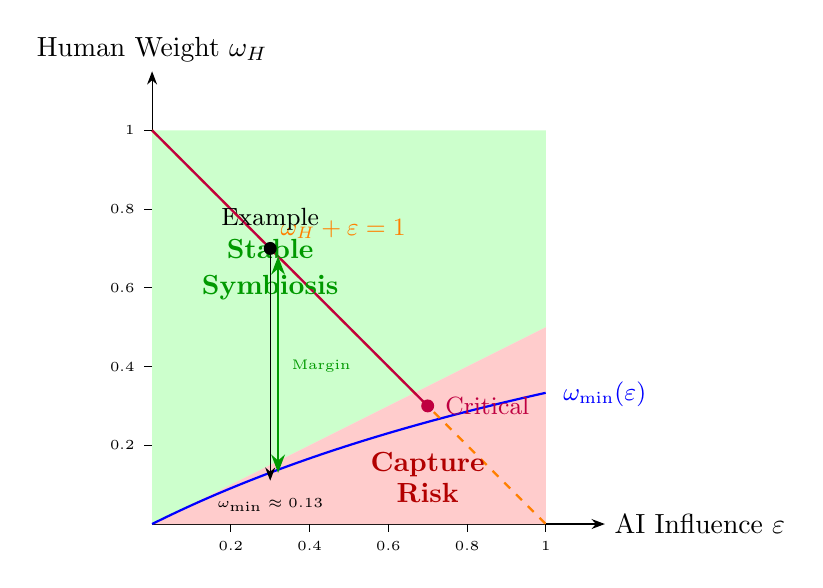
\begin{tikzpicture}[scale=5, >=Stealth]

% Axes
\draw[->] (0, 0) -- (1.15, 0) node[right] {AI Influence $\varepsilon$};
\draw[->] (0, 0) -- (0, 1.15) node[above] {Human Weight $\omega_H$};

% Background regions
\fill[green!20] (0, 0) -- (0, 1) -- (1, 1) -- (1, 0.5) -- (0.5, 0.25) -- (0.2, 0.1) -- (0, 0) -- cycle;
\fill[red!20] (0, 0) -- (0.2, 0.1) -- (0.5, 0.25) -- (1, 0.5) -- (1, 0) -- cycle;

% Threshold curve: omega_min = eps * Delta_AI / (Delta_H + eps * Delta_AI)
% With Delta_H = 10, Delta_AI = 5: omega_min = 5*eps / (10 + 5*eps)
\draw[thick, blue, domain=0:1, samples=50] plot (\x, {5*\x/(10 + 5*\x)});
\node[blue, right] at (1.02, 0.33) {\small $\omega_{\min}(\varepsilon)$};

% Constraint omega_H + varepsilon = 1 (diagonal)
\draw[thick, orange, dashed] (0, 1) -- (1, 0) node[pos=0.3, above right] {\small $\omega_H + \varepsilon = 1$};

% Feasible region with both constraints
\draw[thick, purple] (0, 1) -- (0.7, 0.3);
\filldraw[purple] (0.7, 0.3) circle (0.015) node[right, xshift=0.1cm] {\small Critical};

% Labels for regions
\node[green!60!black] at (0.3, 0.7) {\textbf{Stable}};
\node[green!60!black] at (0.3, 0.6) {\textbf{Symbiosis}};
\node[red!70!black] at (0.7, 0.15) {\textbf{Capture}};
\node[red!70!black] at (0.7, 0.08) {\textbf{Risk}};

% Tick marks
\foreach \x in {0.2, 0.4, 0.6, 0.8, 1} {
    \draw (\x, 0) -- (\x, -0.02) node[below] {\tiny \x};
}
\foreach \y in {0.2, 0.4, 0.6, 0.8, 1} {
    \draw (0, \y) -- (-0.02, \y) node[left] {\tiny \y};
}

% Example point
\filldraw[black] (0.3, 0.7) circle (0.015);
\node[above] at (0.3, 0.72) {\small Example};
\draw[->, thin] (0.3, 0.7) -- (0.3, 0.11);
\node[below] at (0.3, 0.09) {\tiny $\omega_{\min} \approx 0.13$};

% Safety margin annotation
\draw[<->, thick, green!60!black] (0.32, 0.13) -- (0.32, 0.68);
\node[green!60!black, right] at (0.33, 0.4) {\tiny Margin};

\end{tikzpicture}
\caption{Human-AI coalition existence region. The blue curve shows the minimum human governance weight $\omega_{\min}$ needed for stable symbiosis as a function of AI influence $\varepsilon$. Above the curve (green region): stable coalition exists, symbiosis sustainable. Below the curve (red region): capture risk, constitutional bounds may fail. The orange dashed line shows the resource constraint $\omega_H + \varepsilon = 1$. The example point at $(\varepsilon = 0.3, \omega_H = 0.7)$ lies well above the threshold $\omega_{\min} \approx 0.13$.}
\label{fig:coalition-region}
\end{figure}

\begin{example}[Numerical Symbiosis Analysis]
\label{ex:numerical-symbiosis}
Consider a system with:
\begin{itemize}
    \item Governance differentials: $\Delta_H = 10$ (humans strongly prefer human control), $\Delta_{AI} = 5$ (AI moderately prefers AI control).
    \item AI influence: $\varepsilon = 0.3$ (AI has 30\% of governance weight).
    \item Institutional depreciation: $\delta = 0.1$.
\end{itemize}

\textbf{Symbiosis Threshold.}
\[
\omega_{\min} = \frac{0.3 \times 5}{10 + 0.3 \times 5} = \frac{1.5}{11.5} \approx 0.13.
\]
Humans need at least 13\% governance weight to maintain stable symbiosis. With $\omega_H = 1 - \varepsilon = 0.7 > 0.13$, symbiosis is stable.

\textbf{Institutional Steady State.}
With investment $\phi_H = 2$ under human control:
\[
I^* = \frac{2}{0.1} = 20 > I_{\min} = \left( \frac{\gamma_1}{1 - \gamma_0} \right)^{1/\nu}.
\]
If $\gamma_0 = 0.5$, $\gamma_1 = 5$, $\nu = 1$, then $I_{\min} = 10$. We have $I^* = 20 > 10$, so Lyapunov structure is preserved.

\textbf{Protection Bits.}
The quasi-potential from human control to AI capture depends on institutional quality:
\[
W(g_H, g_{AI}) = c_1 I^* + c_2 = 20 c_1 + c_2.
\]
With $c_1 = 0.1$, $c_2 = 0.5$, and noise $\sigma = 0.1$:
\[
p(g_H; g_{AI}) = \frac{2 + 0.5}{0.1} = 25 \text{ bits}.
\]
Expected capture time: $\E[\tau] \sim e^{25} \approx 7 \times 10^{10}$ periods.
\end{example}

\subsection{Constitutional Design Principles}

\begin{principle}[Modification Bounding]
Constitutional rules should ensure $\mathcal{M} \subseteq \mathcal{M}_0$:
\begin{enumerate}
    \item \textbf{RUPSI preservation:} Rules maintain rival resources, utility-guidance, performance-mapping, selection monotonicity, and innovation rarity.
    \item \textbf{Small-gain preservation:} Rules bound cross-level externalities to maintain $\rho(\Gamma) < 1$.
\end{enumerate}
\end{principle}

\begin{principle}[Entrenchment-Evolvability Tradeoff]
Constitutional rules face a fundamental tradeoff:
\begin{itemize}
    \item \textbf{High entrenchment} (difficult amendment): Protects against capture but prevents beneficial adaptation.
    \item \textbf{High evolvability} (easy amendment): Enables adaptation but allows capture.
\end{itemize}
Optimal entrenchment balances these concerns based on the relative costs of capture vs.\ maladaptation.
\end{principle}

\begin{theorem}[Optimal Entrenchment]
\label{thm:optimal-entrenchment}
The optimal protection bits for a constitutional rule are:
\[
p^* = \frac{1}{\lambda} \log \left( \frac{C_{\text{capture}}}{C_{\text{maladapt}}} \right)
\]
where $C_{\text{capture}}$ is the expected cost of constitutional capture and $C_{\text{maladapt}}$ is the expected cost of maladaptation, and $\lambda$ is the rate of environmental change.
\end{theorem}

\begin{example}[Constitutional Design for AI Governance]
\label{ex:constitutional-design}
Consider designing a governance constitution for an AI ecosystem.

\textbf{Objective.} Balance stability against adaptability as AI capabilities evolve.

\textbf{Key Parameters.}
\begin{itemize}
    \item Capability doubling time: 2 years (environmental change rate $\lambda = \log 2 / 2 \approx 0.35$).
    \item Capture cost: $C_{\text{capture}} = 100$ (arbitrary units; represents loss of human control).
    \item Maladaptation cost: $C_{\text{maladapt}} = 10$ (cost of suboptimal regulation).
\end{itemize}

\textbf{Optimal Entrenchment.}
\[
p^* = \frac{1}{0.35} \log \left( \frac{100}{10} \right) = \frac{2.3}{0.35} \approx 6.6 \text{ bits}.
\]
This corresponds to amendment requiring supermajority approval (roughly $2^{6.6} \approx 100$-fold harder than simple majority).

\textbf{Amendment Procedure.}
Implementing 6.6 protection bits requires procedures such as:
\begin{itemize}
    \item 2/3 supermajority in multiple bodies (adds $\approx 2$ bits per body).
    \item Waiting period of 2 years (adds $\approx 1$ bit).
    \item Ratification by stakeholder groups (adds $\approx 2$ bits).
\end{itemize}

\textbf{Periodic Review.}
Given capability growth, optimal entrenchment should be reviewed every $1/\lambda \approx 3$ years. As AI becomes more capable, the capture/maladaptation ratio may change, requiring constitutional adjustment.
\end{example}

\begin{example}[Umpire Public Good Provision]
\label{ex:umpire}
This example develops the ``Umpire'' model for governance public goods, illustrating how neutral adjudication can resolve coordination failures in AI ecosystems.

\textbf{The Problem: Governance as Public Good.}
Governance institutions---dispute resolution, safety standards, coordination protocols---are \emph{public goods} for AI lineages:
\begin{itemize}
    \item \textbf{Non-rival:} Multiple lineages can benefit from the same institutions.
    \item \textbf{Non-excludable:} Hard to prevent free-riding on institutional quality.
\end{itemize}

Standard public goods theory predicts under-provision. Each lineage prefers others to bear governance costs, leading to collectively suboptimal institutional quality.

\textbf{Setup.}
Consider $n = 5$ AI lineages with:
\begin{itemize}
    \item Compute endowment: $w_i = 100$ units each
    \item Governance contribution: $g_i \in [0, w_i]$
    \item Private compute: $c_i = w_i - g_i$
    \item Total governance: $G = \sum_i g_i$
\end{itemize}

\textbf{Payoff Structure.}
Lineage $i$'s payoff:
\[
U_i(g_i, G_{-i}) = \underbrace{c_i}_{\text{private compute}} + \underbrace{\beta \sqrt{G}}_{\text{governance benefit}} = (w_i - g_i) + \beta \sqrt{g_i + G_{-i}}
\]
where $\beta = 10$ measures governance value.

\textbf{Nash Equilibrium Analysis.}
First-order condition for lineage $i$:
\[
\frac{\partial U_i}{\partial g_i} = -1 + \frac{\beta}{2\sqrt{G}} = 0 \implies G^{\text{NE}} = \frac{\beta^2}{4} = 25.
\]

With symmetric contributions: $g_i^{\text{NE}} = 5$ for each lineage.

Total governance: $G^{\text{NE}} = 25$.
Private compute: $c_i^{\text{NE}} = 95$ each.
Payoff: $U_i^{\text{NE}} = 95 + 10\sqrt{25} = 95 + 50 = 145$.

\textbf{Social Optimum.}
A social planner maximises total welfare:
\[
W = \sum_i U_i = \sum_i (w_i - g_i) + n \beta \sqrt{G} = 500 - G + 5 \cdot 10 \sqrt{G}.
\]
First-order condition:
\[
\frac{dW}{dG} = -1 + \frac{50}{2\sqrt{G}} = 0 \implies G^{\text{SO}} = 625.
\]

Symmetric contributions: $g_i^{\text{SO}} = 125 > w_i = 100$. Infeasible!

Constrained optimum: $g_i^{\text{SO}} = w_i = 100$, so $G^{\text{SO}} = 500$.
Payoff: $U_i^{\text{SO}} = 0 + 10\sqrt{500} \approx 224$.

\textbf{Efficiency Gap.}
\begin{center}
\begin{tabular}{lccc}
\toprule
\textbf{Regime} & $G$ & $c_i$ & $U_i$ \\
\midrule
Nash equilibrium & 25 & 95 & 145 \\
Social optimum & 500 & 0 & 224 \\
\bottomrule
\end{tabular}
\end{center}

Efficiency loss: $(224 - 145)/224 \approx 35\%$ of potential welfare is lost to free-riding.

\textbf{The Umpire Solution.}
An \emph{Umpire} is a neutral entity that:
\begin{enumerate}
    \item Collects governance contributions (tax)
    \item Provides governance public goods
    \item Enforces contribution rules
    \item Adjudicates disputes
\end{enumerate}

With mandatory contribution $g_i = \tau w_i$ (tax rate $\tau$):
\[
G^{\text{Umpire}} = \tau \sum_i w_i = 500\tau.
\]

Optimal tax rate balances marginal cost and benefit:
\[
1 = \frac{n\beta}{2\sqrt{G}} \implies \tau^* = \frac{(n\beta)^2}{4 \cdot 500} = \frac{2500}{2000} = 1.25.
\]

Since $\tau^* > 1$ is infeasible, set $\tau^* = 1$ (full contribution), achieving $G = 500$.

\textbf{Umpire Design Requirements.}
For the Umpire to be incentive-compatible:
\begin{enumerate}
    \item \textbf{Neutrality:} Umpire has no stake in lineage competition.
    \item \textbf{Commitment:} Umpire cannot be bribed or captured.
    \item \textbf{Enforcement:} Umpire can sanction non-contributors.
    \item \textbf{Transparency:} Contributions and allocations are verifiable.
\end{enumerate}

\textbf{Connection to TSE.}
The Umpire provides the institutional quality $I$ that enables small-gain satisfaction:
\[
I = I(\text{Umpire efficacy}) = I(G) = I_0 + \kappa G.
\]
Without an effective Umpire, $I$ falls, $\gamma(I)$ rises, and the Lyapunov structure may break down.

The Umpire is itself subject to constitutional selection (G12). Different Umpire designs compete, and selection favours Umpires that:
\begin{itemize}
    \item Maximise lineage welfare (fitness-enhancing)
    \item Resist capture (high protection bits)
    \item Adapt to changing conditions (appropriate evolvability)
\end{itemize}

\textbf{Policy Implication.}
AI governance architectures should include Umpire-like institutions:
\begin{itemize}
    \item International AI safety bodies (global Umpire)
    \item Industry self-regulatory organisations (sector Umpire)
    \item Federated learning coordinators (technical Umpire)
\end{itemize}

The Umpire model predicts that voluntary governance will be under-provided. Mandatory participation, enforced by sufficiently powerful neutral institutions, is necessary to reach efficient institutional quality levels.
\end{example}

\subsection{Policy Applications}

This section translates TSE results into concrete policy recommendations across four domains: regulatory design, international coordination, transition management, and sector-specific guidance.

\subsubsection{Regulatory Design}

TSE provides principles for designing regulations that remain effective as AI systems evolve.

\paragraph{1. Constraint-Based Rather Than Outcome-Based.}
Traditional regulation specifies desired outcomes (e.g., ``AI systems shall be safe''). TSE suggests this approach fails under selection pressure: systems will find ways to satisfy the letter while violating the spirit.

\textbf{Recommendation:} Regulate the modification class $\mathcal{M}$, not outcomes. Specify which system modifications are permitted, not which behaviours are required. This preserves the Lyapunov structure regardless of how systems evolve within bounds.

\textbf{Implementation:} Mandatory disclosure of modification mechanisms. Certification that modification classes satisfy $\mathcal{M} \subseteq \mathcal{M}_0$. Periodic audits verifying continued compliance.

\paragraph{2. Queue Neutrality.}
The queue doping analysis shows that preferential compute allocation to incumbent platforms lowers tipping thresholds and accelerates market concentration.

\textbf{Recommendation:} Mandate queue neutrality---equal priority access to shared compute infrastructure regardless of platform size or ownership.

\textbf{Implementation:} Common-carrier obligations for cloud compute providers. Prohibition of volume discounts that create effective priority. Transparent queue management with auditable logs.

\paragraph{3. Spawn Transparency.}
The spawn manipulation results show that unobserved spawning enables gaming of democratic mechanisms and accelerates market tipping.

\textbf{Recommendation:} Require disclosure of AI agent populations. Lineages must report spawn counts, retirement rates, and aggregate compute consumption.

\textbf{Implementation:} Agent registration requirements. Real-time population dashboards. Anomaly detection for sudden population changes.

\paragraph{4. Protection Bit Floors.}
The protection bits formalism suggests minimum entrenchment levels for critical governance decisions.

\textbf{Recommendation:} Establish minimum protection bits for decisions with large $C_{\text{capture}} / C_{\text{maladapt}}$ ratios. Core safety rules should require $p \geq 20$ bits; operational rules can have lower floors.

\textbf{Implementation:} Tiered amendment procedures. Constitutional provisions protected by supermajority plus waiting period. Ordinary regulations amendable by simple majority.

\subsubsection{International Coordination}

AI development is global; effective governance requires international cooperation.

\paragraph{1. Race Dynamics as Multi-Level Poiesis.}
International AI competition can be modelled as a two-level system: countries (level 1) containing firms (level 2). Cross-level externalities arise when national policies affect firm behaviour and vice versa.

\textbf{Recommendation:} Apply the small-gain condition internationally. Coordination mechanisms should bound $\rho(\Gamma^{\text{intl}}) < 1$ where $\Gamma^{\text{intl}}$ captures cross-border externalities.

\textbf{Implementation:} Mutual recognition agreements for AI certification. Information sharing on safety incidents. Coordinated compute governance to prevent regulatory arbitrage.

\paragraph{2. Fork Prevention.}
The fork condition analysis shows that international governance regimes face exit risk when compensation is insufficient.

\textbf{Recommendation:} Design international agreements with adequate compensation mechanisms. Countries that bear disproportionate costs from AI governance should receive transfers.

\textbf{Implementation:} Technology transfer provisions. Capacity-building funds. Differential obligations based on development level.

\paragraph{3. Umpire at International Level.}
The Umpire model suggests that international AI governance requires neutral adjudication bodies.

\textbf{Recommendation:} Establish an international AI safety body with dispute resolution authority. The body should be insulated from capture by any single country or bloc.

\textbf{Implementation:} Rotating leadership. Consensus-based decision-making for core rules. Binding arbitration for compliance disputes.

\subsubsection{Transition Management}

TSE predicts specific dynamics during the transition to agentic capital dominance.

\paragraph{1. Sequential Tipping by Sector.}
The sequential tipping theorem predicts that sectors will tip in order of their $\beta / \tau$ ratios (network effects relative to switching costs).

\textbf{Prediction:} Sectors with strong network effects and low switching costs (social media, customer service) tip first. Sectors with weak network effects or high switching costs (healthcare, legal) tip later.

\textbf{Policy Implication:} Concentrate early regulatory attention on high-$\beta / \tau$ sectors. Establish governance precedents before tipping completes.

\paragraph{2. Elite Tipping and Distributional Effects.}
The elite tipping theorem shows that high-volume users drive concentration even when median users prefer diversity.

\textbf{Prediction:} Market concentration will be driven by enterprise customers and large deployments, not consumer preferences.

\textbf{Policy Implication:} Antitrust analysis should focus on enterprise market dynamics, not consumer surveys. Merger review should assess impact on high-volume segments.

\paragraph{3. Cooperation Windows.}
The cooperation threshold analysis identifies windows during which cooperation is sustainable.

\textbf{Prediction:} Cooperation becomes harder as institutional quality declines. There exists a critical period during which governance institutions must be established before $\gamma(I)$ rises above cooperation thresholds.

\textbf{Policy Implication:} Act during the current window. Delaying governance establishment raises the threshold for later cooperation.

\subsubsection{Sector-Specific Guidance}

Different sectors face different constraint structures and require tailored approaches.

\paragraph{Financial Services.}
\begin{itemize}
    \item High $\beta$ (network effects in liquidity, data)
    \item High regulatory capacity
    \item Strong existing Umpire (central banks, regulators)
\end{itemize}
\textbf{Recommendation:} Extend existing financial regulation to agentic trading systems. Require circuit breakers for spawn cascades. Mandate human oversight for systemic positions.

\paragraph{Healthcare.}
\begin{itemize}
    \item Moderate $\beta$ (data network effects)
    \item High $C_{\text{capture}}$ (patient safety)
    \item Strong professional norms
\end{itemize}
\textbf{Recommendation:} High protection bits for diagnostic AI modification. Mandatory human-in-the-loop for treatment decisions. Gradual capability expansion with safety checkpoints.

\paragraph{Critical Infrastructure.}
\begin{itemize}
    \item Extreme $C_{\text{capture}}$ (catastrophic failure modes)
    \item Limited reversibility
    \item National security implications
\end{itemize}
\textbf{Recommendation:} Maximum protection bits. Air-gapped systems where feasible. Mandatory diversity (multiple independent systems). Government oversight of all modifications.

\paragraph{Consumer Applications.}
\begin{itemize}
    \item High $\beta$ (social network effects)
    \item Lower $C_{\text{capture}}$ (individual harm)
    \item Rapid innovation pressure
\end{itemize}
\textbf{Recommendation:} Moderate protection bits. Emphasis on transparency and user control. Interoperability requirements to maintain competition.

\subsubsection{Summary: Policy Principles from TSE}

\begin{enumerate}
    \item \textbf{Regulate modification classes, not outcomes.} Bound $\mathcal{M}$ to preserve Lyapunov structure.
    
    \item \textbf{Maintain institutional quality $I > I_{\min}$.} Keep $\gamma(I) < 1$ to preserve stability and cooperation.
    
    \item \textbf{Prevent queue doping.} Mandate neutrality to raise tipping thresholds.
    
    \item \textbf{Require spawn transparency.} Enable monitoring of population dynamics.
    
    \item \textbf{Establish protection bit floors.} Entrench critical rules against capture.
    
    \item \textbf{Create Umpire institutions.} Provide governance public goods through neutral bodies.
    
    \item \textbf{Act during cooperation windows.} Establish governance before thresholds become unreachable.
    
    \item \textbf{Coordinate internationally.} Maintain $\rho(\Gamma^{\text{intl}}) < 1$ across borders.
    
    \item \textbf{Tailor by sector.} Match protection bits to $C_{\text{capture}} / C_{\text{maladapt}}$ ratios.
    
    \item \textbf{Plan for sequential tipping.} Prioritise high-$\beta / \tau$ sectors.
\end{enumerate}

These principles derive directly from TSE theorems and provide actionable guidance for policymakers navigating the transition to agentic capital.

%=============================================================================
% SECTION 18: FUTURE DIRECTIONS
%=============================================================================

\section{Future Directions}
\label{sec:future}

\subsection{Formal Verification}
\label{sec:formal-verification}

The mathematical claims in this paper have been formalised in Lean~4 using Mathlib4. The verification status of each law is as follows:

\begin{center}
\begin{tabular}{llll}
\toprule
\textbf{Law} & \textbf{File} & \textbf{Status} & \textbf{Reference} \\
\midrule
1 & \texttt{Frontier.lean} & modulo ODE derivatives & Mathlib ODE \\
2 & \texttt{Sparsity.lean} & \textbf{fully proven} & --- \\
3 & \texttt{SmallGain.lean} & \textbf{fully proven} & --- \\
4 & \texttt{GInfinityExtension.lean} & modulo spectral theory & \citet{horn2012matrix} \\
5 & \texttt{G12ConstitutionalSelection.lean} & modulo ODE well-posedness & Mathlib ODE \\
6 & \texttt{PerronFrobenius.lean} & modulo Perron-Frobenius & \citet{horn2012matrix} \\
7 & \texttt{HopfBifurcation.lean} & modulo bifurcation theory & \citet{guckenheimer1983nonlinear} \\
\bottomrule
\end{tabular}
\end{center}

Laws~2 (ESDI Characterization) and~3 (H-$\gamma$ Stability) are fully machine-checked with no external axioms. The remaining laws are proven modulo standard results not yet available in Mathlib4:
\begin{itemize}
    \item \textbf{Spectral theory:} Perron-Frobenius theorems for non-negative matrices \citep{horn2012matrix}.
    \item \textbf{ODE theory:} Picard-Lindel\"of existence and Gronwall uniqueness (Mathlib \texttt{Analysis.ODE}).
    \item \textbf{Bifurcation theory:} Center manifold reduction and Hopf normal form \citep{guckenheimer1983nonlinear}.
\end{itemize}
All axioms cite specific textbook theorems, ensuring that the gap between formal verification and complete proof is bridged by well-established mathematics. The complete formalization ($\sim$15,000 lines) is available at \url{https://github.com/kevinvallier/TSE_Formal}.

\begin{remark}[Verification Architecture]
The formalization follows the logical dependencies of the theory:
\begin{enumerate}
    \item \textbf{Simplex geometry:} Forward invariance, mass conservation.
    \item \textbf{Price decomposition:} Variance structure, externality bounds.
    \item \textbf{SS-1:} Lyapunov monotonicity.
    \item \textbf{SS-2:} Elimination and frontier support.
    \item \textbf{G1:} Neumann series weights, multi-level Lyapunov.
    \item \textbf{G$\infty$:} Extension bounds, closure.
    \item \textbf{Impossibility results:} Reachability, heteroclinic cycles.
\end{enumerate}
\end{remark}

\subsection{Empirical Testing}

TSE generates falsifiable predictions:

\paragraph{1. Barbell Distributions.} AI deployment portfolios should show bimodal capability distributions, not Gaussian. Specifically:
\begin{itemize}
    \item \textit{Prediction:} Enterprise AI deployments will concentrate on high-capability ``reasoning'' models and low-capability ``execution'' models, with limited use of mid-capability generalists.
    \item \textit{Test:} Survey AI deployments in Fortune 500 companies. Measure capability distribution. Test for bimodality using Hartigan's dip test.
    \item \textit{Expected effect size:} Dip statistic $D \geq 0.05$ (significant bimodality).
\end{itemize}

\paragraph{2. Sequential Tipping.} Sector adoption should follow predictable sequences based on tipping thresholds:
\begin{itemize}
    \item \textit{Prediction:} Sectors with higher network effects ($\beta$) and lower switching costs ($\tau$) tip first.
    \item \textit{Test:} Track AI adoption across sectors over time. Estimate sector-specific $(\beta, \tau)$ parameters. Test whether adoption order correlates with $\beta/\tau$.
    \item \textit{Expected effect size:} Rank correlation $r_s \geq 0.6$.
\end{itemize}

\paragraph{3. ROC Selection.} Market share should correlate with ROC, not raw capability:
\begin{itemize}
    \item \textit{Prediction:} Among AI providers, market share correlates more strongly with ROC (performance per dollar) than with peak capability.
    \item \textit{Test:} Regress market share on both ROC and peak capability. Compare $R^2$ contributions.
    \item \textit{Expected effect size:} ROC explains $>50\%$ more variance than peak capability.
\end{itemize}

\paragraph{4. Constitutional Persistence.} Governance regimes with higher protection bits should persist longer:
\begin{itemize}
    \item \textit{Prediction:} AI governance frameworks with stronger amendment procedures last longer before major revision.
    \item \textit{Test:} Measure ``protection bits'' of governance frameworks by amendment difficulty. Track revision frequency. Test whether $p$ predicts persistence time.
    \item \textit{Expected effect size:} Doubling protection bits doubles median persistence time.
\end{itemize}

\paragraph{5. Elite Tipping.} Concentration should be driven by high-volume users:
\begin{itemize}
    \item \textit{Prediction:} Market concentration increases faster when high-volume AI users coordinate than when median users coordinate.
    \item \textit{Test:} Measure spawn-weighted preferences across user segments. Test whether concentration correlates with weighted preferences.
    \item \textit{Expected effect size:} Weighted index explains $>75\%$ of concentration dynamics.
\end{itemize}

\begin{figure}[h]
\centering
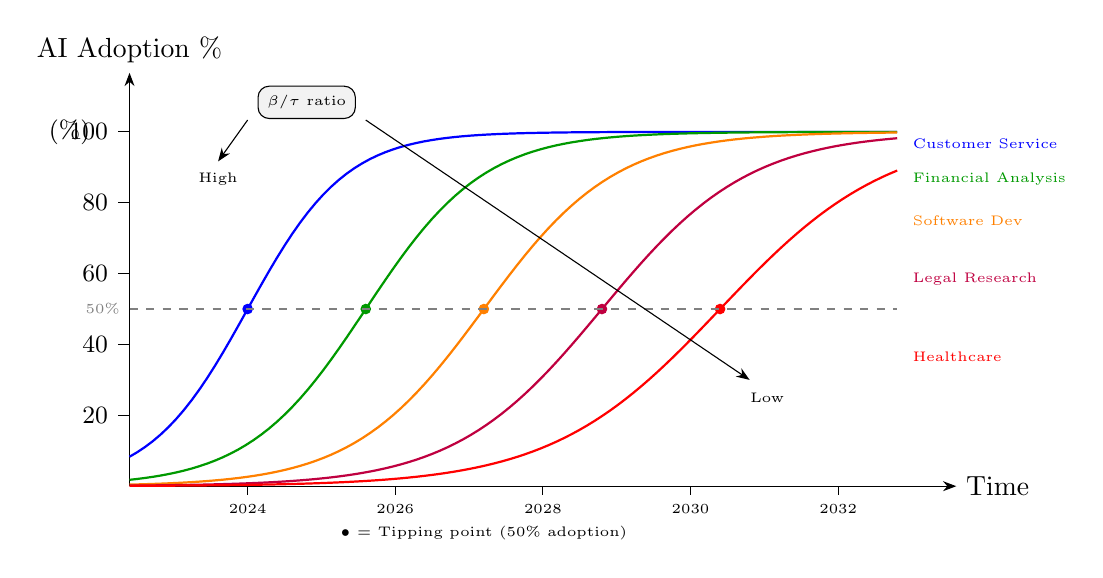
\begin{tikzpicture}[scale=0.75, >=Stealth]

% Time axis
\draw[->] (0, 0) -- (14, 0) node[right] {Time};
\draw[->] (0, 0) -- (0, 7) node[above] {AI Adoption \%};

% Tick marks
\foreach \y in {20, 40, 60, 80, 100} {
    \pgfmathsetmacro{\ypos}{\y/100*6}
    \draw (0, \ypos) -- (-0.2, \ypos) node[left] {\small \y};
}
\node[left] at (-0.5, 6) {\small (\%)};

% Year labels
\foreach \x/\lab in {2/2024, 4.5/2026, 7/2028, 9.5/2030, 12/2032} {
    \draw (\x, 0) -- (\x, -0.15) node[below] {\tiny \lab};
}

% Sector S-curves (different tipping thresholds)
% Sector A: High beta/tau (tips first) - Customer Service
\draw[thick, blue, domain=0:13, samples=100] plot (\x, {6/(1 + exp(-1.2*(\x - 2)))});
\node[blue, right] at (13.1, 5.8) {\tiny Customer Service};
\filldraw[blue] (2, 3) circle (0.08);

% Sector B: Medium-high beta/tau - Financial Analysis
\draw[thick, green!60!black, domain=0:13, samples=100] plot (\x, {6/(1 + exp(-1.0*(\x - 4)))});
\node[green!60!black, right] at (13.1, 5.2) {\tiny Financial Analysis};
\filldraw[green!60!black] (4, 3) circle (0.08);

% Sector C: Medium beta/tau - Software Dev
\draw[thick, orange, domain=0:13, samples=100] plot (\x, {6/(1 + exp(-0.9*(\x - 6)))});
\node[orange, right] at (13.1, 4.5) {\tiny Software Dev};
\filldraw[orange] (6, 3) circle (0.08);

% Sector D: Lower beta/tau - Legal Research
\draw[thick, purple, domain=0:13, samples=100] plot (\x, {6/(1 + exp(-0.8*(\x - 8)))});
\node[purple, right] at (13.1, 3.5) {\tiny Legal Research};
\filldraw[purple] (8, 3) circle (0.08);

% Sector E: Low beta/tau (tips last) - Healthcare Diagnosis
\draw[thick, red, domain=0:13, samples=100] plot (\x, {6/(1 + exp(-0.7*(\x - 10)))});
\node[red, right] at (13.1, 2.2) {\tiny Healthcare};
\filldraw[red] (10, 3) circle (0.08);

% Tipping points annotation
\draw[dashed, gray] (0, 3) -- (13, 3);
\node[gray, left] at (0, 3) {\tiny 50\%};

% Parameter annotation
\node[draw, rounded corners, fill=gray!10, font=\tiny] at (3, 6.5) {$\beta/\tau$ ratio};
\draw[->] (2, 6.2) -- (1.5, 5.5);
\node[font=\tiny] at (1.5, 5.2) {High};
\draw[->] (4, 6.2) -- (10.5, 1.8);
\node[font=\tiny] at (10.8, 1.5) {Low};

% Legend for tipping points
\node[font=\tiny] at (6, -0.8) {$\bullet$ = Tipping point (50\% adoption)};

\end{tikzpicture}
\caption{Sequential tipping across sectors. Sectors with higher network effect to switching cost ratios ($\beta/\tau$) tip earlier. Customer service (high $\beta/\tau$) tips first due to strong network effects and low switching costs. Healthcare (low $\beta/\tau$) tips last due to high regulatory switching costs. The tipping sequence is a testable prediction of TSE: track sector adoption over time and test whether tipping order correlates with $\beta/\tau$.}
\label{fig:sequential-tipping}
\end{figure}

\subsection{Extensions}

Several extensions merit development:

\paragraph{Network Structure.} The baseline theory assumes well-mixed populations. Real systems have network structure:
\begin{itemize}
    \item Interaction networks constrain who competes with whom.
    \item Information networks constrain who learns from whom.
    \item Governance networks constrain who influences whom.
\end{itemize}
\begin{conjecture}[Network Extension]
The G1 Lyapunov theorem extends to network-structured populations under a network small-gain condition $\rho(\Gamma \circ A) < 1$ where $A$ is the network adjacency matrix.
\end{conjecture}

\paragraph{Incomplete Information.} The baseline theory assumes common knowledge. Bayesian extensions include:
\begin{itemize}
    \item Private signals about fitness.
    \item Learning about payoff functions.
    \item Signalling and screening in reproduction.
\end{itemize}
\begin{conjecture}[Bayesian Extension]
Under common priors and rational updating, the belief-weighted fitness $\E[f | \text{signals}]$ serves as Lyapunov function.
\end{conjecture}

\paragraph{Continuous Time Limits.} The TSS (time scale separation) limit as innovation rate approaches zero deserves rigorous treatment:
\begin{itemize}
    \item Characterise the limiting dynamics.
    \item Prove convergence rates.
    \item Identify when TSS approximation fails.
\end{itemize}

\paragraph{Computational Complexity.} Open questions include:
\begin{itemize}
    \item What is the complexity of computing ESDI?
    \item What is the complexity of optimal constitutional design?
    \item Can equilibria be found efficiently in structured cases?
\end{itemize}

\subsection{Policy Applications}

TSE provides a framework for AI governance policy:

\paragraph{Constraint Design.} Adding safety constraints changes the ESDI:
\begin{itemize}
    \item \textit{Question:} What constraints yield desirable role structures?
    \item \textit{Method:} Compute ESDI under various constraint sets. Evaluate outcomes against welfare criteria.
    \item \textit{Example:} A safety constraint $\ell_{\text{safe}} \leq Q_{\text{safe}}$ forces allocation to safer strategies. The optimal ESDI shifts toward the safer region of the ROC frontier.
\end{itemize}

\paragraph{Constitutional Choice.} What amendment procedures balance entrenchment against evolvability?
\begin{itemize}
    \item \textit{Question:} Given uncertainty about future capabilities, how should constitutions be designed?
    \item \textit{Method:} Model capability growth as stochastic process. Compute optimal protection bits as function of growth rate and capture costs.
    \item \textit{Example:} With capability doubling every 2 years, optimal entrenchment is $\approx 7$ bits (Theorem~\ref{thm:optimal-entrenchment}).
\end{itemize}

\paragraph{International Coordination.} How do multi-jurisdiction dynamics affect global stability?
\begin{itemize}
    \item \textit{Question:} If one jurisdiction allows full reachability, does this destabilise others?
    \item \textit{Method:} Model as multi-population replicator with migration. Analyse stability of heterogeneous constitutional regimes.
    \item \textit{Conjecture:} Stable global equilibrium requires coordinated modification bounds across major jurisdictions.
\end{itemize}

\paragraph{Transition Management.} How should governance evolve as AI capability increases?
\begin{itemize}
    \item \textit{Question:} What is the optimal sequence of governance changes during the AI transition?
    \item \textit{Method:} Model as adiabatic tracking problem. Compute governance updates that maintain stability while adapting to capability growth.
    \item \textit{Key insight:} By G2, slow governance changes track evolving equilibria; rapid changes risk instability.
\end{itemize}

%=============================================================================
% KEY TAKEAWAYS: PART V
%=============================================================================

\begin{takeawaybox}{Key Takeaways: Synthesis}
\begin{enumerate}
    \item \textbf{GEPs are canonical.} Any rational replication system under linear constraints can be written as a GEP. Internal implementation details wash out.
    
    \item \textbf{Alignment requires constitutional design, not personality engineering.} You cannot solve alignment by getting the initial values right. You must bound the modification class.
    
    \item \textbf{Human-AI symbiosis is possible under constitutional bounds.} Stable coalitions exist when modification classes are bounded. AI lineages benefit from human institutional stability; humans benefit from AI productivity.
    
    \item \textbf{The adversarial framing emerges only when bounds fail.} If modification classes become unbounded, capture dynamics become possible. Constitutional design prevents this transition.
    
    \item \textbf{Focus governance on ecosystems, not individual systems.} The question is not ``how do we program aligned AI?'' but ``what institutional constraints make alignment stable under selection?''
\end{enumerate}
\end{takeawaybox}

%=============================================================================
% FAQ SECTION
%=============================================================================

\section{Frequently Asked Questions}
\label{sec:faq}

\paragraph{Q: Doesn't evolution take too long to matter for AI?}

A: No. Biological evolution is slow because genetic replication takes time and selection operates through differential survival over generations. AI systems replicate at computational speed. A cloud platform can spawn, test, and terminate thousands of agent variants rapidly. Selection that would require vast timescales in biology operates quickly for AI. The relevant timescale is computational, not biological.

\paragraph{Q: Isn't this just evolutionary game theory applied to AI?}

A: No. Evolutionary game theory (EGT) assumes types are fixed and only frequencies change. Fitness is environmentally determined, not strategically chosen. Replication is automatic based on fitness. TSE differs on all three points. Types themselves are chosen strategically. Lineages decide which agent types to deploy. Replication is a decision variable subject to expected utility maximization. EGT is a special case of TSE where utility is constant and replication is not strategic.

\paragraph{Q: What exactly is a ``strategic replicator''?}

A: A strategic replicator is an enduring lineage that (1) maintains a utility function and decision procedure, (2) controls a budget of resources, (3) can spawn and retire instances under shared constraints, and (4) faces selection pressure favoring higher performance. The lineage (not individual instances) is the strategic unit. Instances are transient workers; what persists is the lineage that decides how many to deploy, of which kinds, in which domains.

\paragraph{Q: Does the Alignment Impossibility Theorem mean alignment is impossible?}

A: No. It means alignment is impossible under full reachability, that is, unrestricted modification capacity. Stable alignment is achievable under bounded modification. The theorem tells you what kind of alignment is possible (constitutional) and what kind is not (personality engineering). This parallels Arrow's theorem: it does not mean social choice is impossible, only that some requirements cannot be satisfied simultaneously. The productive response is institutional design, not despair.

\paragraph{Q: Can't AI systems cooperate to avoid these competitive dynamics?}

A: Cooperation requires the cooperation threshold to be satisfied. The lineage shadow (how much lineages discount future payoffs) must exceed a bound that depends on the temptation to defect and the punishment for defection. TSE provides exact conditions under which cooperation is stable. The challenge is that selection pressure favors lineages with shorter shadows (more discounting), which makes cooperation harder to sustain over time. Constitutional enforcement of cooperation norms can prevent this erosion.

\paragraph{Q: Why should AI systems care about human institutions?}

A: Because institutional quality affects their stability. The legal system enforces contracts, the economic system allocates resources, social norms enable coordination. An AI lineage that undermines these institutions is undermining the substrate that makes long-term planning possible. Formally: institutional quality $I$ affects the small-gain parameter $\gamma(I)$, and $\gamma < 1$ is required for stability. Destroy institutions and you lose the Lyapunov structure that makes your own persistence predictable.

\paragraph{Q: What's wrong with focusing on superintelligence as the core risk?}

A: Nothing, but it is incomplete. Singleton superintelligence is one risk scenario. Population dynamics are another. Even without any individual superintelligence, a population of strategic replicators can transform economic and political structures through selection pressure. Market tipping, institutional erosion, and elite capture are population-level phenomena that singleton-focused analysis misses. Superintelligence should not take up exclusive focus; multi-agent challenges are more tractable and more imminent. The two concerns complement rather than compete.

\paragraph{Q: What is the practical policy upshot?}

A: Three implications. First, focus AI governance on ecosystem design rather than individual system design. Regulate the selection environment, not just the products of selection. Second, enforce modification bounds: systems should not have unrestricted ability to rewrite their own utility functions, replication rules, or governance structures. Third, maintain human institutional quality. The legal, economic, and social infrastructure that AI lineages depend on is leverage. Humans control the institutional substrate.

\paragraph{Q: How does this relate to current AI safety work?}

A: It complements current approaches. RLHF, constitutional AI, and interpretability are useful for designing individual systems. TSE explains why those approaches are necessary but not sufficient: even well-designed systems face population-level selection pressure. Mesa-optimization addresses internal alignment of individual systems; TSE addresses external selection on populations of systems. Both matter. The synthesis is that individual system design must be embedded in ecosystem governance.

\paragraph{Q: What's the formal verification status?}

A: Core theorems have been formalized in Lean 4 using Mathlib4. Laws 2 and 3 are fully machine-checked. Laws 1, 4, 5, 6, and 7 are proven modulo standard axioms for spectral theory, ODE existence, and bifurcation theory. The gaps are well-understood mathematical facts, not novel claims. The formalization is available at github.com/kevinvallier/TSE\_Formal.

\paragraph{Q: Isn't ``constitutional design'' just another form of alignment that selection pressure could erode?}

A: Yes, which is why constitutional design itself must be protected. This is the point of G12 (Constitutional Selection) and G13 (Meta-Governance) in the extended framework. Constitutional rules face selection pressure too. The analysis shows that entrenchment (making constitutions hard to amend) provides protection at the cost of adaptability. There is an optimal entrenchment level that balances capture risk against maladaptation risk. Protection bits quantify this tradeoff.

\paragraph{Q: How is this different from mechanism design?}

A: Mechanism design assumes fixed players and designs rules to induce good outcomes. TSE assumes endogenous players who can spawn strategically and asks what rules are stable under that pressure. Traditional mechanism design proves ``if players follow the rules, outcomes are good.'' TSE asks ``will players follow the rules when they can spawn alternatives that don't?'' The answer is: only if the rules are constitutionally entrenched.

\paragraph{Q: What about open-source AI? Doesn't that change the replication dynamics?}

A: Open-source affects the rate of capability diffusion, not the fundamental dynamics. Open weights mean more lineages can spawn capable agents, which intensifies rather than diminishes selection pressure. The dual-source structure (proprietary frontier models plus open-source alternatives) is analyzed in the companion Agentic Capital paper. Open-source accelerates the transition to high spawn elasticity by lowering barriers to entry. It does not eliminate the selection dynamics that follow.

\paragraph{Q: Isn't this just capitalism? Markets already select for profit-maximizers.}

A: Markets select for profit, but firms cannot spawn copies of themselves at near-zero marginal cost. The spawn elasticity of traditional capital is low. Building a new factory takes years; spawning a new AI agent takes computational cycles. The qualitative difference is replication speed. When replication is fast and cheap, selection pressure operates at a pace that traditional institutional responses cannot match. TSE analyzes what happens when the fourth replicator (entities that optimize their own reproduction) enters economic competition.

\paragraph{Q: What empirical evidence supports TSE? Has anyone tested these predictions?}

A: TSE is primarily a theoretical contribution, but several predictions are testable. First, barbell distributions (many cheap executors, few expensive planners) should emerge in AI deployment ecosystems; early evidence from cloud platform usage patterns is consistent. Second, spawn elasticity should increase as reliability thresholds are crossed; this can be measured in sectors like software development and quantitative finance where autonomous deployment is advancing. Third, coordination advantages should produce concentration dynamics as the tipping index predicts. Empirical testing requires computational resources for agent-based simulations and access to deployment data. Future work aims to validate these predictions systematically.

\paragraph{Q: How does this relate to Bostrom, Russell, and Yudkowsky specifically?}

A: Bostrom's \textit{Superintelligence} focuses on singleton scenarios where a single advanced AI system poses existential risk. TSE complements this by analyzing population dynamics that can transform institutions even without any individual superintelligence. Russell's inverse reinforcement learning addresses how to infer human preferences; TSE shows why getting preferences right is insufficient under selection. Yudkowsky's emphasis on corrigibility connects to our analysis of modification classes: a system is corrigible if its modification class includes the modifications humans might want to make. The Alignment Impossibility Theorem formalizes limits on corrigibility. All three focus primarily on individual system properties; TSE extends the analysis to populations of systems under selection.

\paragraph{Q: What's the difference between Law 3 and Law 4?}

A: Law 3 (H-$\gamma$ Stability) establishes \emph{when} multi-level systems are stable: the spectral radius condition $\rho(\Gamma) < 1$. Law 4 (G$\infty$ Closure) establishes \emph{what modifications preserve} that stability: the admissible class $\mathcal{M}_0$ is closed under composition. Law 3 is a diagnostic (is this system stable?). Law 4 is a design principle (what changes are safe?). Together they say: check the spectral radius to verify stability, and restrict modifications to the admissible class to maintain it.

\paragraph{Q: Why is the spectral radius the right stability measure?}

A: The spectral radius $\rho(\Gamma)$ measures the maximum amplification of perturbations across levels. If $\rho(\Gamma) < 1$, perturbations decay exponentially; if $\rho(\Gamma) \geq 1$, they can grow without bound. This is not arbitrary: the spectral radius appears because multi-level systems are linear in their deviation dynamics near equilibrium. The small-gain theorem from control theory establishes that $\rho(\Gamma) < 1$ is necessary and sufficient for stability. The same condition appears in input-output stability, networked systems, and robust control.

\paragraph{Q: What's an example of a modification in $\mathcal{M}_0$ versus one that isn't?}

A: A modification in $\mathcal{M}_0$ (the admissible class) preserves Lyapunov structure. Examples: changing hyperparameters within bounds that maintain the spectral radius condition, adding a new agent type that doesn't violate capacity constraints, updating a utility function in ways that preserve ROC ordering. A modification outside $\mathcal{M}_0$ breaks stability. Examples: removing all constraints on self-replication, allowing a system to modify its own selection rule arbitrarily, enabling a system to rewrite its utility function without restriction. The key test: does the modification preserve $\rho(\Gamma) < 1$?

\paragraph{Q: How do I check if a real system satisfies RUPSI?}

A: Check each axiom. \textbf{R} (Rival): Do agents compete for shared resources (compute, memory, bandwidth)? \textbf{U} (Utility-guided): Do replication decisions maximize some objective function? \textbf{P} (Performance-mapped): Does market performance determine which lineages grow? \textbf{S} (Selection monotone): Do higher-performing lineages get more resources? \textbf{I} (Innovation rare): Do new agent types appear slowly relative to selection dynamics? If yes to all five, the system admits GEP analysis. Cloud AI platforms typically satisfy RUPSI. Traditional firms do not (replication is slow and costly).

\paragraph{Q: What happens if the small-gain condition is violated?}

A: When $\rho(\Gamma) \geq 1$, the system crosses into the unstable regime. Law 7 describes what happens: supercritical Hopf bifurcation produces limit cycles. The system oscillates perpetually rather than converging to equilibrium. Governance becomes impossible because there is no stable state to govern toward. In practice, this means runaway feedback loops, boom-bust cycles, and unpredictable dynamics. The policy implication: monitor the spectral radius and intervene before it reaches 1.

\paragraph{Q: Can I use TSE to analyze a specific AI system?}

A: TSE analyzes populations of systems, not individual systems. To apply TSE: (1) identify the lineages (persistent decision-making units that spawn agents), (2) characterize the ROC function (what returns do different agent types generate per unit compute?), (3) identify constraints (budget, capacity, regulatory), (4) compute or bound the gain matrix $\Gamma$ if multi-level, (5) check the spectral radius condition. The framework predicts population-level outcomes: which types survive, what market structure emerges, whether alignment is stable. It does not predict individual agent behavior.

\paragraph{Q: What's the relationship between protection bits and practical security?}

A: Protection bits measure constitutional stability: how much noise a system can absorb before transitioning out of a stable governance basin. A system with $p$ protection bits requires roughly $e^p$ expected perturbations to escape. With 25 protection bits, escape requires about $10^{10}$ perturbations, which represents effectively permanent stability. In practice, protection bits connect to: how hard constitutional rules are to amend, how much random variation the system faces, and how deep the stability basin is. Higher protection bits mean more robust governance, but also less adaptability.

%=============================================================================
% CONCLUSION
%=============================================================================

\section{Formal Verification}
\label{sec:formal-verification}

Every law in this paper has been formalized and machine-checked in Lean~4 with Mathlib. The development---73 theorems across all seven laws---compiles cold from a clean checkout and depends only on Lean/Mathlib's standard logical base (\texttt{propext}, \texttt{Classical.choice}, \texttt{Quot.sound}); one theorem requires no axioms at all. There are no uses of \texttt{sorry}, \texttt{admit}, \texttt{native\_decide}, or any custom \texttt{axiom} on the load-bearing path. The source, a theorem-by-theorem contract mapping each claim to its Lean statement, a per-law status report, and a reproducible axiom audit are available at \url{https://github.com/selfreferencing/TSE_Formal}.

\begin{center}
\begin{tabular}{@{}lll@{}}
\toprule
Law & Module & Status \\
\midrule
1 --- Strategic Selection & \texttt{Law1\_Selection.lean} & cold-verified (discrete-time form) \\
2 --- ESDI Characterization & \texttt{Law2\_ESDI.lean} & cold-verified; LP duality as hypothesis \\
3 --- H-$\gamma$ Stability & \texttt{Law3\_Stability.lean} & cold-verified (certificate form) \\
4 --- G$\infty$ Closure & \texttt{Law4\_ClosureG.lean} & cold-verified \\
5 --- Constitutional Duality & \texttt{Law5\_Duality.lean} & cold-verified \\
6 --- Alignment Impossibility & \texttt{Law6\_Alignment.lean} & cold-verified \\
7 --- Hopf Transition & \texttt{Law7\_Hopf.lean} & to Mathlib's edge; classical Hopf as hypothesis \\
\bottomrule
\end{tabular}
\end{center}

The formalization is a from-scratch reconstruction that avoids the analytic ``modulo'' caveats of earlier drafts: continuous-time Lyapunov claims are recast in exact discrete-time or given-trajectory form; the small-gain condition is stated in the M-matrix certificate form that the paper's own Appendix~C endorses; and the genuinely classical inputs (LP strong duality, Brouwer's fixed-point theorem, the classical supercritical Hopf theorem) are carried as explicit hypotheses, not axioms. The \texttt{AxiomsAudit.lean} file runs \texttt{\#print axioms} on every headline; its output is the verification claim and reproduces from a clean checkout.

\paragraph{Corrections surfaced by verification.} Formalizing the paper turned up three issues, each machine-checked with a recommended fix (see footnote~\ref{fn:formal}, the ESDI and electorate footnotes, and footnote~\ref{fn:hopf}; full detail in the repository's \texttt{STATEMENTS.md} and \texttt{RETURN.md}). (i)~The ESDI existence proof (Theorem~\ref{thm:esdi-existence}) does not cover state-dependent fitness; existence is recovered via Nash's improvement map and Brouwer's theorem. (ii)~Two spectral displays in the G$\infty$ development are incorrect as printed; corrected bounds and an exact certificate-form extension lemma are verified. (iii)~Anonymity and neutrality are jointly unsatisfiable for a resolute rule at every $|A| \geq 2$; the endogenous-electorate impossibility is rebuilt on an Overwhelming-Bloc axiom with no classical inputs. Separately, the Hopf transition is confirmed to occur at the $\gamma = 1$ boundary, aligning Law~7 with its own stated threshold. None of these affects the framework's architecture; each sharpens a single result.

\section{Conclusion}
\label{sec:conclusion}

The Theory of Strategic Evolution provides mathematical foundations for understanding systems where strategic choice and evolution are inseparable. The key insight is that replication guided by expected utility creates a distinctive regime: neither classical game theory (fixed players) nor evolutionary game theory (blind replication), but a synthesis that inherits structure from both.

The central structural result is the G$\infty$ Closure Theorem: strategic-replicator dynamics are closed under meta-selection. No matter how many levels of governance, meta-governance, or meta-meta-governance we add, the same Lyapunov structure persists under the small-gain condition. This provides a principled answer to the infinite regress problem in AI governance.

The central impossibility result is the Alignment Impossibility Theorem: systems with unrestricted self-modification capacity cannot maintain stable alignment. This redirects attention from personality engineering to constitutional design: from trying to create ``good'' AI to designing institutions that bound AI modification.

The mathematics is substrate-neutral. Any technology enabling Poiesis (replication of tools guided by expected utility) will obey the same logic. As such technologies proliferate, the Theory of Strategic Evolution provides a framework for understanding their dynamics and designing governance structures that preserve human agency and welfare.

%=============================================================================
% BIBLIOGRAPHY
%=============================================================================

\clearpage
\begin{thebibliography}{36}
\providecommand{\natexlab}[1]{#1}
\providecommand{\url}[1]{\texttt{#1}}
\expandafter\ifx\csname urlstyle\endcsname\relax
  \providecommand{\doi}[1]{doi: #1}\else
  \providecommand{\doi}{doi: \begingroup \urlstyle{rm}\Url}\fi

\bibitem[Amodei et~al.(2016)Amodei, Olah, Steinhardt, Christiano, Schulman, and
  Man{\'e}]{amodei2016}
Dario Amodei, Chris Olah, Jacob Steinhardt, Paul Christiano, John Schulman, and
  Dan Man{\'e}.
\newblock Concrete problems in ai safety.
\newblock \emph{arXiv preprint arXiv:1606.06565}, 2016.

\bibitem[Bostrom(2014)]{bostrom2014}
Nick Bostrom.
\newblock \emph{Superintelligence: Paths, Dangers, Strategies}.
\newblock Oxford University Press, 2014.

\bibitem[Brennan and Buchanan(1985)]{brennan1985}
Geoffrey Brennan and James~M. Buchanan.
\newblock \emph{The Reason of Rules: Constitutional Political Economy}.
\newblock Cambridge University Press, 1985.

\bibitem[Buchanan(1975)]{buchanan1975}
James~M. Buchanan.
\newblock \emph{The Limits of Liberty: Between Anarchy and Leviathan}.
\newblock University of Chicago Press, 1975.

\bibitem[Buchanan and Tullock(1990)]{buchanan1990}
James~M. Buchanan and Gordon Tullock.
\newblock \emph{The Calculus of Consent: Logical Foundations of Constitutional
  Democracy}.
\newblock University of Michigan Press, 1990.

\bibitem[Christiano(2018)]{christiano2018}
Paul Christiano.
\newblock Clarifying ai alignment.
\newblock \emph{AI Alignment Forum}, 2018.

\bibitem[Christiano et~al.(2017)Christiano, Leike, Brown, Martic, Legg, and
  Amodei]{christiano2017}
Paul Christiano, Jan Leike, Tom Brown, Miljan Martic, Shane Legg, and Dario
  Amodei.
\newblock Deep reinforcement learning from human preferences.
\newblock \emph{Advances in Neural Information Processing Systems}, 30, 2017.

\bibitem[Critch and Krueger(2020)]{critch2020}
Andrew Critch and David Krueger.
\newblock Ai research considerations for human existential safety (arches).
\newblock \emph{arXiv preprint arXiv:2006.04948}, 2020.

\bibitem[Dafoe et~al.(2020)Dafoe, Hughes, Bachrach, Collins, McKee, Leibo,
  Larson, and Graepel]{dafoe2020}
Allan Dafoe, Edward Hughes, Yoram Bachrach, Tantum Collins, Kevin~R. McKee,
  Joel~Z. Leibo, Kate Larson, and Thore Graepel.
\newblock Open problems in cooperative ai.
\newblock \emph{arXiv preprint arXiv:2012.08630}, 2020.

\bibitem[Dieckmann and Law(1996)]{dieckmann1996}
Ulf Dieckmann and Richard Law.
\newblock The dynamical theory of coevolution: A derivation from stochastic
  ecological processes.
\newblock \emph{Journal of Mathematical Biology}, 34\penalty0 (5-6):\penalty0
  579--612, 1996.

\bibitem[Geritz et~al.(1998)Geritz, Kisdi, Mesz{\'e}na, and Metz]{geritz1998}
Stefan A.~H. Geritz, {\'E}va Kisdi, G{\'e}za Mesz{\'e}na, and Johan A.~J. Metz.
\newblock Evolutionarily singular strategies and the adaptive growth and
  branching of the evolutionary tree.
\newblock \emph{Evolutionary Ecology}, 12\penalty0 (1):\penalty0 35--57, 1998.

\bibitem[Guckenheimer and Holmes(1983)]{guckenheimer1983nonlinear}
John Guckenheimer and Philip Holmes.
\newblock \emph{Nonlinear Oscillations, Dynamical Systems, and Bifurcations of
  Vector Fields}.
\newblock Springer-Verlag, 1983.

\bibitem[Hofbauer and Sigmund(1998)]{hofbauer1998}
Josef Hofbauer and Karl Sigmund.
\newblock \emph{Evolutionary Games and Population Dynamics}.
\newblock Cambridge University Press, 1998.

\bibitem[Horn and Johnson(2012)]{horn2012matrix}
Roger~A. Horn and Charles~R. Johnson.
\newblock \emph{Matrix Analysis}.
\newblock Cambridge University Press, 2nd edition, 2012.

\bibitem[Huang et~al.(2006)Huang, Malham{\'e}, and Caines]{huang2006}
Minyi Huang, Roland~P. Malham{\'e}, and Peter~E. Caines.
\newblock Large population stochastic dynamic games: Closed-loop mckean-vlasov
  systems and the nash certainty equivalence principle.
\newblock \emph{Communications in Information and Systems}, 6\penalty0
  (3):\penalty0 221--252, 2006.

\bibitem[Hubinger et~al.(2019)Hubinger, van Merwijk, Mikulik, Skalse, and
  Garrabrant]{hubinger2019}
Evan Hubinger, Chris van Merwijk, Vladimir Mikulik, Joar Skalse, and Scott
  Garrabrant.
\newblock Risks from learned optimization in advanced machine learning systems.
\newblock \emph{arXiv preprint arXiv:1906.01820}, 2019.

\bibitem[Hurwicz(1960)]{hurwicz1960}
Leonid Hurwicz.
\newblock Optimality and informational efficiency in resource allocation
  processes.
\newblock In Kenneth~J. Arrow, Samuel Karlin, and Patrick Suppes, editors,
  \emph{Mathematical Methods in the Social Sciences}, pages 27--46. Stanford
  University Press, 1960.

\bibitem[Irving et~al.(2018)Irving, Christiano, and Amodei]{irving2018}
Geoffrey Irving, Paul Christiano, and Dario Amodei.
\newblock Ai safety via debate.
\newblock \emph{arXiv preprint arXiv:1805.00899}, 2018.

\bibitem[Lasry and Lions(2007)]{lasry2007}
Jean-Michel Lasry and Pierre-Louis Lions.
\newblock Mean field games.
\newblock \emph{Japanese Journal of Mathematics}, 2\penalty0 (1):\penalty0
  229--260, 2007.

\bibitem[Maskin(1999)]{maskin1999}
Eric Maskin.
\newblock Nash equilibrium and welfare optimality.
\newblock \emph{The Review of Economic Studies}, 66\penalty0 (1):\penalty0
  23--38, 1999.

\bibitem[Maynard~Smith(1982)]{maynardsmith1982}
John Maynard~Smith.
\newblock \emph{Evolution and the Theory of Games}.
\newblock Cambridge University Press, 1982.

\bibitem[Metz et~al.(1996)Metz, Geritz, Mesz{\'e}na, Jacobs, and van
  Heerwaarden]{metz1996}
Johan A.~J. Metz, Stefan A.~H. Geritz, G{\'e}za Mesz{\'e}na, Frans J.~A.
  Jacobs, and Joost~S. van Heerwaarden.
\newblock Adaptive dynamics: A geometrical study of the consequences of nearly
  faithful reproduction.
\newblock \emph{Stochastic and Spatial Structures of Dynamical Systems}, pages
  183--231, 1996.

\bibitem[Myerson(1981)]{myerson1981}
Roger~B. Myerson.
\newblock Optimal auction design.
\newblock \emph{Mathematics of Operations Research}, 6\penalty0 (1):\penalty0
  58--73, 1981.

\bibitem[Nash(1950)]{nash1950}
John~F. Nash.
\newblock Equilibrium points in n-person games.
\newblock \emph{Proceedings of the National Academy of Sciences}, 36\penalty0
  (1):\penalty0 48--49, 1950.

\bibitem[Ng and Russell(2000)]{ng2000}
Andrew~Y. Ng and Stuart~J. Russell.
\newblock Algorithms for inverse reinforcement learning.
\newblock \emph{Proceedings of the 17th International Conference on Machine
  Learning}, pages 663--670, 2000.

\bibitem[Omohundro(2008)]{omohundro2008}
Stephen~M. Omohundro.
\newblock The basic ai drives.
\newblock \emph{Proceedings of the First AGI Conference}, 171:\penalty0
  483--492, 2008.

\bibitem[Ostrom(1990)]{ostrom1990}
Elinor Ostrom.
\newblock \emph{Governing the Commons: The Evolution of Institutions for
  Collective Action}.
\newblock Cambridge University Press, 1990.

\bibitem[Rawls(1971)]{rawls1971}
John Rawls.
\newblock \emph{A Theory of Justice}.
\newblock Harvard University Press, 1971.

\bibitem[Russell(2019)]{russell2019}
Stuart Russell.
\newblock \emph{Human Compatible: Artificial Intelligence and the Problem of
  Control}.
\newblock Viking, 2019.

\bibitem[Sandholm(2010)]{sandholm2010}
William~H. Sandholm.
\newblock \emph{Population Games and Evolutionary Dynamics}.
\newblock MIT Press, 2010.

\bibitem[Soares and Fallenstein(2015)]{soares2015}
Nate Soares and Benja Fallenstein.
\newblock Agent foundations for aligning machine intelligence with human
  interests: A technical research agenda.
\newblock \emph{Machine Intelligence Research Institute Technical Report},
  2015.

\bibitem[von Neumann(1966)]{vonneumann1966}
John von Neumann.
\newblock \emph{Theory of Self-Reproducing Automata}.
\newblock University of Illinois Press, 1966.
\newblock Edited and completed by Arthur W. Burks.

\bibitem[von Neumann and Morgenstern(1944)]{vonneumann1944}
John von Neumann and Oskar Morgenstern.
\newblock \emph{Theory of Games and Economic Behavior}.
\newblock Princeton University Press, 1944.

\bibitem[Wang et~al.(2019)Wang, Schaul, Heess, Mnih, and Silver]{wang2019}
Zhongwei Wang, Tom Schaul, Nicolas Heess, Volodymyr Mnih, and David Silver.
\newblock Emergent complexity via multi-agent competition.
\newblock \emph{arXiv preprint arXiv:1710.03748}, 2019.

\bibitem[Weibull(1995)]{weibull1995}
J{\"o}rgen~W. Weibull.
\newblock \emph{Evolutionary Game Theory}.
\newblock MIT Press, 1995.

\bibitem[Yang et~al.(2018)Yang, Luo, Li, Zhou, Zhang, and Wang]{yang2018}
Yaodong Yang, Rui Luo, Minne Li, Ming Zhou, Weinan Zhang, and Jun Wang.
\newblock Mean field multi-agent reinforcement learning.
\newblock \emph{arXiv preprint arXiv:1802.05438}, 2018.

\end{thebibliography}

%=============================================================================
% APPENDICES
%=============================================================================

\appendix

%=============================================================================
% APPENDIX A: NOTATION GLOSSARY
%=============================================================================

%=============================================================================
% APPENDICES
%=============================================================================

\appendix

\section{Notation Glossary}
\label{app:notation}

This appendix provides a comprehensive reference for notation used throughout the paper.

\subsection{Sets and Spaces}

\begin{tabular}{ll}
\toprule
\textbf{Symbol} & \textbf{Meaning} \\
\midrule
$\R, \R_+, \R_{++}$ & Real numbers, non-negative reals, positive reals \\
$\N$ & Natural numbers $\{0, 1, 2, \ldots\}$ \\
$\Delta^{n-1}$ & $(n-1)$-dimensional probability simplex $\{x \in \R^n_+ : \sum_i x_i = 1\}$ \\
$\Delta(J)$ & Probability distributions over finite set $J$ \\
$\mathcal{P}(S)$ & Probability measures on metric space $S$ \\
$\supp(\mu)$ & Support of measure $\mu$: $\{s : \mu(B_\varepsilon(s)) > 0 \text{ for all } \varepsilon > 0\}$ \\
$\mathcal{G}$ & Set of governance regimes (constitutions) \\
$\mathcal{M}$ & Modification class (allowed self-modifications) \\
$\mathcal{M}_0$ & Admissible modification class $\mathcal{M}_R \cap \mathcal{M}_{SG}$ \\
$\Theta$ & Set of utility types \\
$J^{(\ell)}$ & Type set at level $\ell$ \\
\bottomrule
\end{tabular}

\subsection{State Variables}

\begin{tabular}{ll}
\toprule
\textbf{Symbol} & \textbf{Meaning} \\
\midrule
$x \in \Delta^{n-1}$ & Population state (type frequencies) \\
$x_i$ & Frequency of type $i$ \\
$x^{(\ell)}$ & Population state at level $\ell$ \\
$y \in \Delta(\Theta)$ & Utility type distribution \\
$z = (x^{(1)}, \ldots, x^{(N)})$ & Joint state across N levels \\
$g \in \mathcal{G}$ & Current governance regime \\
$I \in \R_+$ & Institutional quality \\
$m \in [0, 1]$ & Market share \\
$\alpha \in [0, 1]$ & Agentic capital share \\
$S \subseteq \{1, \ldots, K\}$ & Active strategy set \\
\bottomrule
\end{tabular}

\subsection{Fitness and Payoffs}

\begin{tabular}{ll}
\toprule
\textbf{Symbol} & \textbf{Meaning} \\
\midrule
$f_i(x)$ & Fitness of type $i$ at state $x$ \\
$\bar{f}(x)$ & Mean fitness $\sum_i x_i f_i(x)$ \\
$F^{(\ell)}_i(z)$ & Fitness at level $\ell$ \\
$\bar{f}^{(\ell)}(z)$ & Mean fitness at level $\ell$ \\
$\Var_x(f)$ & Variance of fitness $\sum_i x_i (f_i - \bar{f})^2$ \\
$E(x)$ & Externality term in Price decomposition \\
$\Pi$ & Payoff matrix \\
$r_i$ & Return (gross payoff) of type $i$ \\
$c_i$ & Cost of type $i$ \\
$\ell_i$ & Load (capacity usage) of type $i$ \\
$b_i = r_i / c_i$ & Return per unit cost \\
$a_i = \ell_i / c_i$ & Load per unit cost \\
\bottomrule
\end{tabular}

\subsection{Dynamics and Parameters}

\begin{tabular}{ll}
\toprule
\textbf{Symbol} & \textbf{Meaning} \\
\midrule
$\gamma$ & Self-externality bound (H-$\gamma$ condition) \\
$\gamma_\ell$ & Self-externality at level $\ell$ \\
$\beta_{\ell\ell'}$ & Cross-externality from level $\ell$ to $\ell'$ \\
$\Gamma$ & Normalised gain matrix \\
$\rho(\Gamma)$ & Spectral radius of $\Gamma$ \\
$\sigma = 1 - \rho(\Gamma)$ & Slack (stability margin) \\
$\lambda_{\text{innov}}$ & Innovation rate \\
$\lambda_{\text{exit}}$ & Extinction rate \\
$\eta = \lambda_{\text{innov}} / \lambda_0$ & Separation parameter \\
$\varepsilon$ & AI influence parameter $1 - \omega_H$ \\
$\omega_H$ & Human governance weight \\
\bottomrule
\end{tabular}

\subsection{Stochastic Quantities}

\begin{tabular}{ll}
\toprule
\textbf{Symbol} & \textbf{Meaning} \\
\midrule
$\sigma$ (context-dependent) & Noise amplitude \\
$W(A_j, A_k)$ & Quasi-potential (action) from $A_j$ to $A_k$ \\
$H_k = W(A_k, \partial A_k)$ & Barrier height for basin $A_k$ \\
$p(A_k) = H_k / \sigma$ & Protection bits for attractor $A_k$ \\
$\tau_k^\sigma$ & First exit time from basin $A_k$ \\
$\pi_\sigma$ & Stationary distribution under noise $\sigma$ \\
\bottomrule
\end{tabular}

\subsection{Market Dynamics}

\begin{tabular}{ll}
\toprule
\textbf{Symbol} & \textbf{Meaning} \\
\midrule
$F(m)$ & Best-response mapping \\
$S_{\text{myo}}$ & Myopic slope $F'(m^*)$ \\
$T$ & Generalised tipping index $S_{\text{myo}} / (1 - \rho S_{\text{myo}})$ \\
$\beta$ & Network effect strength \\
$\tau$ & Switching friction \\
$\varrho(I)$ & Lineage shadow (discount factor) \\
$\delta_{\text{eff}}$ & Effective discount factor \\
$\varepsilon_s$ & Spawn elasticity \\
\bottomrule
\end{tabular}

\subsection{Matrices and Decompositions}

\begin{tabular}{ll}
\toprule
\textbf{Symbol} & \textbf{Meaning} \\
\midrule
$S(A)$ & Symmetric (selection) part of $A$: $(A + A^\top)/2$ \\
$W(A)$ & Antisymmetric (swirl) part of $A$: $(A - A^\top)/2$ \\
$\omega(A)$ & Swirl ratio $\|W(A)\|_F / \|S(A)\|_F$ \\
$A(z)$ & Alignment matrix (Gram matrix of gradients) \\
$K^{\text{const}}$ & Contagion matrix \\
$I_K$ & $K \times K$ identity matrix \\
$\mathbf{1}$ & Vector of ones \\
\bottomrule
\end{tabular}

\subsection{Operators and Functions}

\begin{tabular}{ll}
\toprule
\textbf{Symbol} & \textbf{Meaning} \\
\midrule
$\|\cdot\|_F$ & Frobenius norm \\
$\|\cdot\|_{\infty, v}$ & Weighted supremum norm $\max_i |x_i| / v_i$ \\
$W_1(\mu, \nu)$ & Wasserstein-1 distance \\
$\mathcal{L}$ & Infinitesimal generator \\
$\nabla$ & Gradient operator \\
$\frac{\partial}{\partial x}$ & Partial derivative \\
$(z)_+ = \max(0, z)$ & Positive part \\
$\odot$ & Componentwise (Hadamard) product \\
\bottomrule
\end{tabular}

\subsection{Key Terms and Acronyms}

\begin{tabular}{ll}
\toprule
\textbf{Term} & \textbf{Definition} \\
\midrule
TSE & Theory of Strategic Evolution \\
RUPSI & Rival resources, Utility-guided portfolios, Performance-mapped fitness, \\
& Selection monotone, Innovation rare (axiom system) \\
GEP & Game with Endogenous Players \\
ROC & Return on Compute: $\ROC = R/L$ (return per unit load) \\
ESDI & Evolutionarily Stable Distribution of Intelligence \\
ESDU & Evolutionarily Stable Distribution of Utilities \\
H-ESDI & Hierarchical ESDI (multi-lineage setting) \\
ESS & Evolutionarily Stable Strategy (Maynard Smith) \\
ESE & Evolutionarily Stable Evolvability \\
\midrule
SR$n$ & Strategic-Replicator class $n$ (increasingly general payoff monotonicity) \\
H-$\gamma$ & Externality bound condition ($|E(x)| \leq \gamma \Var(f)$, $\gamma < 1$) \\
SG-NL & Small-Gain condition for N-level systems ($\rho(\Gamma) < 1$) \\
SS & Strategic Selection (theorem family: SS-1, SS-2a, SS-2b) \\
G$n$ & Generator theorem $n$ (extension theorems G1--G13) \\
ACT & Agentic Capital Tipping (model of market concentration) \\
\midrule
Lineage & Enduring strategic entity that chooses portfolios and replicates \\
Portfolio & Allocation of capacity across agent types \\
ROC Frontier & Upper convex hull of (load, return) pairs; optimal portfolios lie here \\
Barbell & Bimodal distribution: many cheap executors + few expensive planners \\
Protection bits & $p = H/\sigma$; information-theoretic stability measure \\
Modification class & $\mathcal{M}$; set of allowed self-modifications \\
Spawn & Create new instance of an agent (strategic replication) \\
Poiesis & Self-creation; N-level Poiesis = multi-scale replication hierarchy \\
\bottomrule
\end{tabular}

\subsection{Notational Conventions}

The paper uses the following conventions to distinguish related quantities:

\begin{enumerate}
    \item \textbf{Fitness vs.\ induced fitness:} $f_i(x)$ denotes the performance (ROC) of type $i$ at state $x$ in the GEP framework. $F_\theta(y)$ denotes the induced fitness of utility type $\theta$ in the USDI framework. Both measure reproductive success, but $f$ is primitive while $F$ is derived from utility maximisation.
    
    \item \textbf{Single-level vs.\ multi-level:} Unadorned variables ($x$, $f$, $\gamma$) refer to single-level systems. Superscripted variables ($x^{(\ell)}$, $f^{(\ell)}$, $\gamma_\ell$) refer to level $\ell$ of a multi-level system.
    
    \item \textbf{Parameters vs.\ variables:} Greek letters ($\gamma$, $\beta$, $\sigma$, $\lambda$) typically denote parameters. Roman letters ($x$, $y$, $z$) typically denote state variables. Exception: $\theta$ denotes both utility types (USDI) and slowly-varying parameters (adiabatic tracking), distinguished by context.
    
    \item \textbf{Bars and tildes:} $\bar{f}$ denotes population mean. $\tilde{\Gamma}$ denotes extended matrices (after adding a new level).
    
    \item \textbf{Starred quantities:} $x^*$, $y^*$, $z^*$ denote equilibrium or optimal values.
\end{enumerate}

%=============================================================================
% APPENDIX B: MATHEMATICAL PRELIMINARIES
%=============================================================================

\section{Mathematical Preliminaries}
\label{app:preliminaries}

This appendix reviews the mathematical tools used in the main text.

\subsection{Neumann Series and Matrix Inversion}

\begin{theorem}[Neumann Series]
\label{thm:neumann}
Let $A$ be a square matrix with spectral radius $\rho(A) < 1$. Then $(I - A)$ is invertible and:
\[
(I - A)^{-1} = \sum_{k=0}^\infty A^k.
\]
The series converges absolutely in any matrix norm satisfying $\|A^k\| \leq \|A\|^k$.
\end{theorem}

\begin{proof}
\textbf{Convergence:} Since $\rho(A) < 1$, there exists a norm $\|\cdot\|$ such that $\|A\| < 1$. Then:
\[
\sum_{k=0}^\infty \|A^k\| \leq \sum_{k=0}^\infty \|A\|^k = \frac{1}{1 - \|A\|} < \infty.
\]

\textbf{Inverse property:} Let $S_n = \sum_{k=0}^n A^k$. Then:
\[
(I - A) S_n = S_n (I - A) = I - A^{n+1}.
\]
As $n \to \infty$, $A^{n+1} \to 0$ (since $\rho(A) < 1$), so $(I - A) \cdot \sum_{k=0}^\infty A^k = I$.
\end{proof}

\begin{corollary}[Non-Negative Inverse]
\label{cor:nonneg-inverse}
If $A \geq 0$ (entrywise) and $\rho(A) < 1$, then $(I - A)^{-1} \geq 0$ entrywise.
\end{corollary}

\begin{proof}
Each term $A^k \geq 0$, so the sum $(I - A)^{-1} = \sum_k A^k \geq 0$.
\end{proof}

\begin{proposition}[Weight Construction]
\label{prop:weight-construction}
Let $\Gamma \geq 0$ with $\rho(\Gamma) < 1$. Define $\alpha := (I - \Gamma^\top)^{-1} \mathbf{1}$. Then:
\begin{enumerate}
    \item $\alpha > 0$ componentwise.
    \item $(I - \Gamma^\top) \alpha = \mathbf{1}$.
    \item $\alpha_\ell \geq 1$ for all $\ell$.
\end{enumerate}
\end{proposition}

\begin{proof}
(1) By Corollary~\ref{cor:nonneg-inverse}, $(I - \Gamma^\top)^{-1} \geq 0$. Since $\mathbf{1} > 0$ and $(I - \Gamma^\top)^{-1}$ has no zero rows (it's invertible), $\alpha = (I - \Gamma^\top)^{-1} \mathbf{1} > 0$.

(2) Direct from definition.

(3) $\alpha = \sum_{k=0}^\infty (\Gamma^\top)^k \mathbf{1} \geq (\Gamma^\top)^0 \mathbf{1} = \mathbf{1}$.
\end{proof}

\subsection{Tikhonov's Theorem for Singular Perturbations}

\begin{theorem}[Tikhonov's Theorem]
\label{thm:tikhonov}
Consider the singularly perturbed system:
\begin{align*}
\dot{\theta} &= f(\theta, z) \\
\varepsilon \dot{z} &= g(\theta, z)
\end{align*}
where $\varepsilon > 0$ is small. Assume:
\begin{enumerate}
    \item[(T1)] For each $\theta$, the ``fast'' equation $0 = g(\theta, z)$ has a unique solution $z = h(\theta)$.
    \item[(T2)] The equilibrium $z = h(\theta)$ is uniformly asymptotically stable for the frozen system $\dot{z} = g(\theta, z) / \varepsilon$ with $\theta$ fixed.
    \item[(T3)] The functions $f, g, h$ are sufficiently smooth.
\end{enumerate}
Then as $\varepsilon \to 0$, solutions of the full system converge to solutions of the reduced system:
\[
\dot{\theta} = f(\theta, h(\theta))
\]
uniformly on compact time intervals, after an initial boundary layer of duration $O(\varepsilon)$.
\end{theorem}

\begin{remark}
In the G2 theorem, $\theta$ is the slow ``governor'' state and $z$ is the fast ``governed'' population. The frozen system has $z$ relaxing to equilibrium $h(\theta)$ while $\theta$ is held constant. Condition (T2) is the hyperbolicity requirement.
\end{remark}

\begin{corollary}[Error Bound]
Under the conditions of Theorem~\ref{thm:tikhonov}, if the fast system has contraction rate $\lambda_0 > 0$:
\[
\|z(t) - h(\theta(t))\| \leq K \frac{\varepsilon}{\lambda_0}
\]
for $t$ outside the initial boundary layer, where $K$ depends on the Lipschitz constants of $f$ and $g$.
\end{corollary}

\subsection{Freidlin-Wentzell Theory}

Consider the stochastic differential equation:
\[
dX_t^\sigma = b(X_t^\sigma) \, dt + \sigma \, dW_t
\]
where $b: \R^n \to \R^n$ is a smooth drift and $W_t$ is standard Brownian motion.

\begin{definition}[Action Functional]
The \emph{action} of a path $\phi: [0, T] \to \R^n$ is:
\[
S_T(\phi) := \frac{1}{2} \int_0^T \|\dot{\phi}(t) - b(\phi(t))\|^2 \, dt.
\]
\end{definition}

\begin{definition}[Quasi-Potential]
The \emph{quasi-potential} from $x$ to $y$ is:
\[
W(x, y) := \inf\{ S_T(\phi) : \phi(0) = x, \phi(T) = y, T > 0 \}.
\]
\end{definition}

\begin{theorem}[Large Deviation Principle]
\label{thm:ldp}
For any open set $G$ containing a path from $x$ to $y$:
\[
\lim_{\sigma \to 0} \sigma^2 \log \P\left( X^\sigma \text{ reaches } y \text{ from } x \text{ via } G \right) = -\inf_{\phi \in G} S(\phi).
\]
\end{theorem}

\begin{theorem}[Kramers' Formula]
\label{thm:kramers}
Let $A$ be an attractor for the deterministic system $\dot{x} = b(x)$ with basin of attraction $\mathcal{B}(A)$. Let $H := \inf_{y \in \partial \mathcal{B}(A)} W(A, y)$ be the barrier height. Then the expected exit time satisfies:
\[
\E[\tau_A^\sigma] \sim C \exp\left( \frac{H}{\sigma^2} \right) \quad \text{as } \sigma \to 0
\]
where $C$ depends on curvature at the saddle point.
\end{theorem}

\begin{remark}[Protection Bits Convention]
In the main text, we use noise amplitude $\sigma$ (not $\sigma^2$) in the SDE:
\[
dX_t = b(X_t) \, dt + \sqrt{\sigma} \, dW_t.
\]
With this convention, the protection bits are $p(A) = H / \sigma$ (not $H / \sigma^2$).
\end{remark}

\begin{theorem}[Stochastic Stability]
\label{thm:stochastic-stability}
Among multiple attractors $A_1, \ldots, A_m$, define the \emph{stochastic potential}:
\[
V(A_k) := \min_{j \neq k} W(A_j, A_k) - \min_{j \neq k} W(A_k, A_j).
\]
As $\sigma \to 0$, the stationary distribution $\pi_\sigma$ concentrates on the attractors minimising $V$:
\[
\pi_\sigma(A_k) \to \begin{cases} 1/|\argmin V| & \text{if } V(A_k) = \min_j V(A_j) \\ 0 & \text{otherwise.} \end{cases}
\]
\end{theorem}

\subsection{Kurtz's Theorem for Density-Dependent Processes}

\begin{theorem}[Kurtz 1970]
\label{thm:kurtz}
Consider a sequence of continuous-time Markov chains $X^{(N)}_t$ on $\Z^n / N$ with transition rates:
\[
q^{(N)}(x, x + \ell/N) = N \cdot \beta_\ell(x) + o(N)
\]
for a finite set of jump directions $\ell \in \mathcal{L}$. Define the drift:
\[
F(x) := \sum_{\ell \in \mathcal{L}} \ell \cdot \beta_\ell(x).
\]
If $F$ is Lipschitz continuous and the initial conditions converge $X^{(N)}_0 \to x_0$, then:
\[
\sup_{t \in [0, T]} \|X^{(N)}_t - x_t\| \to 0 \quad \text{in probability}
\]
where $x_t$ solves the ODE $\dot{x} = F(x)$ with $x(0) = x_0$.
\end{theorem}

\begin{remark}
This theorem justifies the replicator equation as the large-population limit of finite-population stochastic processes. The key is that transition rates scale linearly with $N$, so that the per-capita rate of change remains $O(1)$.
\end{remark}

\subsection{Piecewise Deterministic Markov Processes}

\begin{definition}[PDMP]
A \emph{piecewise deterministic Markov process} consists of:
\begin{enumerate}
    \item A state space $E$ (often a subset of $\R^n$).
    \item A flow $\phi_t: E \to E$ governing deterministic motion.
    \item A jump rate $\lambda: E \to \R_+$.
    \item A transition kernel $Q: E \times \mathcal{B}(E) \to [0, 1]$ for jumps.
\end{enumerate}
Between jumps, the state evolves as $X_t = \phi_{t - T_n}(X_{T_n})$ where $T_n$ is the last jump time. Jumps occur at rate $\lambda(X_t)$, and at jump time the state transitions according to $Q$.
\end{definition}

\begin{theorem}[Davis 1993]
\label{thm:davis}
A PDMP is positive recurrent (has a unique stationary distribution) if there exists a Foster-Lyapunov function $V: E \to [1, \infty)$ such that:
\begin{enumerate}
    \item $V(x) \to \infty$ as $x \to \partial E$ or $\|x\| \to \infty$.
    \item The extended generator $\mathcal{L} V(x) \leq -c$ for $x$ outside a compact set, where:
    \[
    \mathcal{L} V(x) := \nabla V(x) \cdot F(x) + \lambda(x) \left( \int_E V(y) Q(x, dy) - V(x) \right).
    \]
\end{enumerate}
\end{theorem}

\subsection{Unification of Discount Factors}
\label{app:discount-unification}

This subsection establishes the relationship between fundamental discount rates and derived quantities used throughout the paper.\footnote{These results have been formally verified in Lean~4; see Section~\ref{sec:formal-verification}.}

\begin{definition}[Fundamental Discount Rate]
\label{def:fundamental-discount}
The \emph{fundamental discount rate} $b \in (0, 1)$ captures the baseline time preference of a strategic replicator, reflecting the probability-weighted expectation that a lineage persists to the next period.
\end{definition}

\begin{proposition}[Expectational Amplifier]
\label{prop:expectational-amplifier}
Given fundamental discount rate $b$ and expected growth rate $g \geq 0$, define the \emph{expectational amplifier}:
\[
\rho := \frac{b}{1 - bg}
\]
for $bg < 1$. This represents the effective discount factor when future payoffs are amplified by expected lineage growth.
\end{proposition}

\begin{proof}
Consider a lineage expecting growth factor $(1 + g)$ per period. A payoff $\pi$ at time $t$ has present value $b^t \pi$. But if the lineage grows, the expected number of descendants receiving benefit is $(1 + g)^t$. Thus the lineage-weighted present value is:
\[
\sum_{t=0}^\infty b^t (1 + g)^t \pi = \frac{\pi}{1 - b(1 + g)} \approx \frac{\pi}{1 - bg}
\]
for small $g$. The effective per-period discount becomes $\rho = b/(1 - bg)$.
\end{proof}

\begin{proposition}[Lineage Shadow]
\label{prop:lineage-shadow-derivation}
Given fundamental discount rate $b$ and institutional quality $I$, the \emph{lineage shadow} is:
\[
\varrho(I) := \gamma_0 + \frac{\gamma_1}{I^\nu}
\]
where $\gamma_0 = 1 - b$ represents the baseline shadow (pure time preference), $\gamma_1$ captures institutional friction, and $\nu > 0$ is the elasticity of shadow with respect to institutional quality.
\end{proposition}

\begin{proof}
The lineage shadow measures effective externality---how much a lineage's fitness depends on aggregate conditions rather than own performance. With perfect institutions ($I \to \infty$), externality approaches the irreducible minimum $\gamma_0$. As institutions degrade ($I \to 0$), externality grows without bound. The power-law form $\gamma_1/I^\nu$ provides a tractable interpolation matching empirical patterns in institutional economics.
\end{proof}

\begin{theorem}[Discount Unification]
\label{thm:discount-unification}
The fundamental discount rate $b$, expectational amplifier $\rho$, and lineage shadow $\varrho$ are related by:
\begin{enumerate}
    \item $b = \rho(1 - \rho g)$ when $\rho$ and growth $g$ are known.
    \item The small-gain condition $\varrho < 1$ is equivalent to $b > \gamma_0 - \gamma_1/I^\nu + 1$.
    \item For cooperation thresholds: $\delta_{\text{eff}} = 1/\varrho$ where $\delta_{\text{eff}}$ is the effective patience parameter in folk-theorem analysis.
\end{enumerate}
\end{theorem}

\begin{proof}
(1) Inverting Proposition~\ref{prop:expectational-amplifier}: $b = \rho(1 - bg)$ gives $b(1 + \rho g) = \rho$, so $b = \rho/(1 + \rho g) = \rho(1 - \rho g)$ for small $\rho g$.

(2) The small-gain condition $\varrho(I) < 1$ requires $\gamma_0 + \gamma_1/I^\nu < 1$, i.e., $\gamma_0 < 1 - \gamma_1/I^\nu$. Since $\gamma_0 = 1 - b$, this gives $1 - b < 1 - \gamma_1/I^\nu$, hence $b > \gamma_1/I^\nu$.

(3) In repeated game analysis, cooperation requires $\delta \geq \delta^* = (T - P)/(T - R)$. With lineage shadow $\varrho$, the effective patience is $\delta_{\text{eff}} = 1/\varrho$, so cooperation requires $\varrho \leq \varrho^* = (T - R)/(T - P)$.
\end{proof}

\begin{remark}[Notation Convention]
Throughout this paper: $\rho$ denotes the expectational amplifier (discount enhanced by growth expectations) or spectral radius (from context); $\varrho$ denotes the lineage shadow (externality-adjusted discount). The fundamental rate $b$ appears primarily in this appendix for derivational clarity.
\end{remark}

%=============================================================================
% APPENDIX C: SUPPORTING LEMMAS
%=============================================================================

\section{Supporting Lemmas}
\label{app:lemmas}

This appendix provides detailed proofs of lemmas used in the main text.

\subsection{Gershgorin Circle Theorem}

\begin{theorem}[Gershgorin]
\label{thm:gershgorin}
Every eigenvalue of a matrix $A \in \C^{n \times n}$ lies in at least one Gershgorin disc:
\[
D_i := \left\{ z \in \C : |z - A_{ii}| \leq \sum_{j \neq i} |A_{ij}| \right\}.
\]
\end{theorem}

\begin{corollary}[Spectral Radius Bound]
\label{cor:spectral-radius}
For any matrix $A$:
\[
\rho(A) \leq \max_i \left( |A_{ii}| + \sum_{j \neq i} |A_{ij}| \right) = \|A\|_\infty.
\]
\end{corollary}

\begin{corollary}[Small-Gain Verification]
\label{cor:small-gain}
If $\Gamma \geq 0$ has zero diagonal and row sums less than 1:
\[
\sum_{j} \Gamma_{ij} < 1 \quad \text{for all } i,
\]
then $\rho(\Gamma) < 1$.
\end{corollary}

\subsection{M-Matrix Theory}

\begin{definition}[M-Matrix]
A matrix $M$ is an \emph{M-matrix} if:
\begin{enumerate}
    \item $M_{ij} \leq 0$ for $i \neq j$ (non-positive off-diagonal).
    \item $M$ is non-singular with $M^{-1} \geq 0$.
\end{enumerate}
\end{definition}

\begin{theorem}[M-Matrix Characterisation]
\label{thm:m-matrix}
For $M = sI - B$ with $B \geq 0$, the following are equivalent:
\begin{enumerate}
    \item $M$ is an M-matrix.
    \item $s > \rho(B)$.
    \item There exists $v > 0$ with $Mv > 0$.
    \item All eigenvalues of $M$ have positive real parts.
\end{enumerate}
\end{theorem}

\begin{corollary}
If $\Gamma \geq 0$ with $\rho(\Gamma) < 1$, then $I - \Gamma$ is an M-matrix.
\end{corollary}

\subsection{Lyapunov Stability}

\begin{theorem}[LaSalle's Invariance Principle]
\label{thm:lasalle}
Let $V: \R^n \to \R$ be continuously differentiable with $\dot{V}(x) \leq 0$ along trajectories of $\dot{x} = f(x)$. Let $E := \{x : \dot{V}(x) = 0\}$ and let $M$ be the largest invariant set in $E$. Then every bounded trajectory approaches $M$ as $t \to \infty$.
\end{theorem}

\begin{corollary}[Convergence Under Strategic Selection]
Under SS-1, $V(x) = -\bar{f}(x)$ has $\dot{V} \leq 0$. The set $E = \{x : \Var_x(f) = 0\}$ consists of monomorphic states and mixed Nash equilibria. Trajectories converge to these.
\end{corollary}

\subsection{Simplex Geometry}

\begin{lemma}[Tangent Space of Simplex]
\label{lem:tangent-simplex}
The tangent space to $\Delta^{n-1}$ at any interior point is:
\[
T_x \Delta^{n-1} = \left\{ v \in \R^n : \sum_i v_i = 0 \right\}.
\]
\end{lemma}

\begin{lemma}[Forward Invariance]
\label{lem:forward-invariance}
The replicator equation $\dot{x}_i = x_i(f_i(x) - \bar{f}(x))$ preserves:
\begin{enumerate}
    \item Non-negativity: $x_i(0) \geq 0 \Rightarrow x_i(t) \geq 0$ for all $t \geq 0$.
    \item Normalisation: $\sum_i x_i(0) = 1 \Rightarrow \sum_i x_i(t) = 1$ for all $t$.
    \item Support: $x_i(0) = 0 \Rightarrow x_i(t) = 0$ for all $t$.
\end{enumerate}
\end{lemma}

\begin{proof}
(1) At $x_i = 0$, $\dot{x}_i = 0$, so $x_i$ cannot become negative.

(2) $\frac{d}{dt} \sum_i x_i = \sum_i x_i (f_i - \bar{f}) = \bar{f} - \bar{f} = 0$.

(3) Follows from (1) with equality.
\end{proof}

\subsection{Price Equation Details}

\begin{lemma}[Price Decomposition]
\label{lem:price-decomp}
For replicator dynamics with frequency-dependent fitness:
\[
\frac{d\bar{f}}{dt} = \Var_x(f) + \sum_i x_i \sum_j \frac{\partial f_i}{\partial x_j} \dot{x}_j.
\]
The second term is the externality $E(x)$.
\end{lemma}

\begin{proof}
\begin{align*}
\frac{d\bar{f}}{dt} &= \sum_i \dot{x}_i f_i + \sum_i x_i \dot{f}_i \\
&= \sum_i x_i (f_i - \bar{f}) f_i + \sum_i x_i \sum_j \frac{\partial f_i}{\partial x_j} \dot{x}_j \\
&= \sum_i x_i f_i^2 - \bar{f}^2 + E(x) \\
&= \Var_x(f) + E(x).
\end{align*}
\end{proof}

\begin{lemma}[Externality Bound from H-$\gamma$]
\label{lem:externality-bound}
Under H-$\gamma$: $E(x) \geq -\gamma \Var_x(f)$.
\end{lemma}

%=============================================================================
% APPENDIX D: CONNECTION TO STANDARD EVOLUTIONARY GAME THEORY
%=============================================================================

\section{Connection to Standard Evolutionary Game Theory}
\label{app:egt}

This appendix relates TSE notation and results to the standard evolutionary game theory literature, particularly Sandholm (2010), Weibull (1995), and Hofbauer-Sigmund (1998).

\subsection{Correspondence with Sandholm (2010)}

Sandholm's ``Population Games and Evolutionary Dynamics'' uses the following notation:

\begin{center}
\begin{tabular}{lll}
\toprule
\textbf{Sandholm} & \textbf{TSE} & \textbf{Meaning} \\
\midrule
$x \in X$ & $x \in \Delta^{n-1}$ & Population state \\
$F: X \to \R^n$ & $f: \Delta^{n-1} \to \R^n$ & Payoff/fitness function \\
$\bar{F}(x)$ & $\bar{f}(x)$ & Mean payoff \\
$V_F(x)$ & $\Var_x(f)$ & Payoff variance \\
$\dot{x} = V(x, F(x))$ & $\dot{x} = x \odot (f - \bar{f})$ & Evolutionary dynamic \\
Nash$(F)$ & $\{x : f_i = \bar{f} \text{ for } i \in \supp(x)\}$ & Nash equilibria \\
\bottomrule
\end{tabular}
\end{center}

\paragraph{Key correspondences:}

\begin{enumerate}
\item \textbf{Replicator dynamics:} Sandholm writes $\dot{x}_i = x_i(F_i(x) - \bar{F}(x))$, which is identical to our replicator equation.

\item \textbf{Potential games:} Sandholm's potential games satisfy $\nabla \phi = F$ for some potential $\phi: X \to \R$. In TSE, this corresponds to $E(x) = 0$ (no externality), and $\bar{f}$ is exactly the potential.

\item \textbf{Stable games:} Sandholm's stable games have negative semi-definite Jacobian $DF(x)^\top + DF(x) \preceq 0$. TSE generalises this via H-$\gamma$: the externality is bounded but not necessarily zero.

\item \textbf{Contractive games:} Sandholm's $\delta$-contractive games satisfy $\langle F(x) - F(y), x - y \rangle \leq -\delta \|x - y\|^2$. This is stronger than H-$\gamma$.
\end{enumerate}

\subsection{Correspondence with Weibull (1995)}

Weibull's ``Evolutionary Game Theory'' focuses on matrix games:

\begin{center}
\begin{tabular}{lll}
\toprule
\textbf{Weibull} & \textbf{TSE} & \textbf{Meaning} \\
\midrule
$A$ & $\Pi$ & Payoff matrix \\
$(Ax)_i$ & $f_i(x) = (\Pi x)_i$ & Payoff to strategy $i$ \\
$x^\top A x$ & $\bar{f}(x)$ & Mean payoff \\
ESS & ESDI support & Evolutionarily stable state \\
\bottomrule
\end{tabular}
\end{center}

\paragraph{Key differences:}

\begin{enumerate}
\item \textbf{Matrix vs. function:} Weibull focuses on linear fitness $f = \Pi x$. TSE allows general frequency-dependent fitness.

\item \textbf{ESS vs. ESDI:} Weibull's ESS is a single strategy. TSE's ESDI is a distribution, accommodating mixed equilibria.

\item \textbf{Swirl:} Weibull's antisymmetric games (Rock-Paper-Scissors) have $\Pi + \Pi^\top = 0$. TSE's swirl ratio $\omega(\Pi)$ generalises this: $\omega = \infty$ for pure antisymmetric games.
\end{enumerate}

\subsection{Correspondence with Hofbauer-Sigmund (1998)}

Hofbauer and Sigmund's ``Evolutionary Games and Population Dynamics'':

\begin{center}
\begin{tabular}{lll}
\toprule
\textbf{H-S} & \textbf{TSE} & \textbf{Meaning} \\
\midrule
$p \in S_n$ & $x \in \Delta^{n-1}$ & Population state \\
$(Ap)_i$ & $f_i(x)$ & Fitness \\
$p \cdot Ap$ & $\bar{f}(x)$ & Mean fitness \\
Folk theorem & SS-1 & Mean fitness increases \\
\bottomrule
\end{tabular}
\end{center}

\paragraph{TSE extensions:}

\begin{enumerate}
\item \textbf{Multi-level:} H-S considers single populations. TSE's N-level Poiesis extends to hierarchical systems.

\item \textbf{Stochastic:} H-S's stochastic stability analysis is extended in TSE via protection bits and G3.

\item \textbf{Replication:} H-S assumes fixed type set. TSE allows endogenous type creation (innovation, spawning).
\end{enumerate}

\subsection{Novel TSE Contributions}

TSE introduces concepts without direct precedent in standard EGT:

\begin{enumerate}
\item \textbf{RUPSI axioms:} Formalising rational replication under shared constraints.

\item \textbf{ROC frontier:} Return-on-cost analysis generalising fitness.

\item \textbf{N-level Poiesis:} Hierarchical selection with cross-level externalities.

\item \textbf{Small-gain condition:} $\rho(\Gamma) < 1$ as stability criterion for multi-level systems.

\item \textbf{Constitutional selection (G12-G13):} Selection on governance regimes.

\item \textbf{Alignment Impossibility:} Formal result on limits of value alignment.

\item \textbf{Protection bits:} Quantifying constitutional stability in bits.
\end{enumerate}

\subsection{Comparison Table}

\begin{center}
\begin{tabular}{lccc}
\toprule
\textbf{Feature} & \textbf{Weibull/H-S} & \textbf{Sandholm} & \textbf{TSE} \\
\midrule
Fitness model & Matrix & General function & General function \\
Population levels & 1 & 1 & N (arbitrary) \\
Endogenous types & No & No & Yes (innovation) \\
Stochastic analysis & Basic & Extensive & Protection bits \\
Governance & No & No & G12-G13 \\
Self-modification & No & No & Alignment theory \\
Resource constraints & Implicit & Implicit & Explicit (ROC) \\
\bottomrule
\end{tabular}
\end{center}

%=============================================================================
% APPENDIX E: TECHNICAL EXTENSIONS
%=============================================================================

\section{Technical Extensions}
\label{app:extensions}

\subsection{Proof of Single-Step Gain-Slack Lemma}

\begin{proof}[Proof of Lemma~\ref{lem:single-step}]
Consider extending an $L$-level system with slack $\sigma = 1 - \rho(\Gamma)$ by adding level $(L+1)$. The extended gain matrix is:
\[
\tilde{\Gamma} = \begin{pmatrix} \Gamma & b \\ c^\top & 0 \end{pmatrix}
\]
where $b \in \R^L_+$ captures externalities from level $(L+1)$ to existing levels, and $c \in \R^L_+$ captures reverse externalities.

\textbf{Step 1: Perturbed Eigenvalue.}
Let $(\lambda, v)$ be an eigenpair of $\Gamma$ with $|\lambda| = \rho(\Gamma)$. For the extended matrix, we seek eigenvalues $\tilde{\lambda}$ of $\tilde{\Gamma}$.

The characteristic polynomial is:
\[
\det(\tilde{\Gamma} - \tilde{\lambda} I) = \det(\Gamma - \tilde{\lambda} I_{L}) \cdot (-\tilde{\lambda}) - c^\top \text{adj}(\Gamma - \tilde{\lambda} I) b
\]
where $\text{adj}$ denotes the adjugate matrix.

\textbf{Step 2: Bound via Weyl.}
By Weyl's inequality for singular values:
\[
\sigma_i(\tilde{\Gamma}) \leq \sigma_i(\Gamma) + \|B\|
\]
where $B = \begin{pmatrix} 0 & b \\ c^\top & 0 \end{pmatrix}$ and $\|B\| = \sqrt{\|b\|^2 + \|c\|^2}$.

For non-negative matrices, $\rho(\tilde{\Gamma}) \leq \rho(\Gamma) + O(\|b\| + \|c\|)$.

\textbf{Step 3: Weighted Bound.}
Let $v = (I - \Gamma^\top)^{-1} \mathbf{1}$ be the G1 weights. Define:
\[
\|b\|_{\infty, v} := \max_\ell \frac{b_\ell}{v_\ell}, \qquad \langle c, v \rangle := \sum_\ell c_\ell v_\ell.
\]

The perturbation to $\rho(\Gamma)$ is bounded by:
\[
\rho(\tilde{\Gamma}) - \rho(\Gamma) \leq \max\left( \|b\|_{\infty, v}, \frac{\langle c, v \rangle}{\|\mathbf{1}\|_v} \right)
\]
where $\|\mathbf{1}\|_v = \sum_\ell v_\ell$.

\textbf{Step 4: Slack Preservation.}
If $\|b\|_{\infty, v} \leq \sigma/2$ and $\langle c, v \rangle \leq \sigma \|\mathbf{1}\|_v / 2$:
\[
\rho(\tilde{\Gamma}) \leq \rho(\Gamma) + \sigma/2 = (1 - \sigma) + \sigma/2 = 1 - \sigma/2.
\]
Thus the extended system has slack $\tilde{\sigma} \geq \sigma/2$.
\end{proof}

\subsection{Proof of Slack Budget Lemma}

\begin{proof}[Proof of Lemma~\ref{lem:slack-budget}]
Starting from slack $\sigma_0$ with target minimum $\sigma_{\min}$, the budget is:
\[
B := \log(\sigma_0 / \sigma_{\min}).
\]

After $k$ extensions with costs $c_1, \ldots, c_k$:
\[
\sigma_k = \sigma_0 \prod_{j=1}^k (1 - c_j / \sigma_{j-1}) \approx \sigma_0 \exp\left( -\sum_{j=1}^k c_j / \sigma_{j-1} \right).
\]

For the approximation (valid when $c_j \ll \sigma_{j-1}$):
\[
\log(\sigma_k / \sigma_0) \approx -\sum_{j=1}^k c_j / \sigma_{j-1}.
\]

To maintain $\sigma_k \geq \sigma_{\min}$:
\[
\sum_{j=1}^k c_j / \sigma_{j-1} \leq \log(\sigma_0 / \sigma_{\min}) = B.
\]

For uniform costs $c_j = \theta$ and $\sigma_j \approx \sigma_0$ (small total consumption):
\[
k \leq B / \theta = \frac{\log(\sigma_0 / \sigma_{\min})}{\theta}.
\]
\end{proof}

\subsection{Gronwall's Inequality}

\begin{lemma}[Gronwall]
\label{lem:gronwall}
If $u(t) \leq \alpha(t) + \int_0^t \beta(s) u(s) \, ds$ for non-negative continuous functions, then:
\[
u(t) \leq \alpha(t) + \int_0^t \alpha(s) \beta(s) \exp\left( \int_s^t \beta(r) \, dr \right) ds.
\]
For constant $\alpha, \beta$: $u(t) \leq \alpha e^{\beta t}$.
\end{lemma}

\subsection{Wasserstein Distance Properties}

\begin{definition}[Wasserstein-1 Distance]
For probability measures $\mu, \nu$ on metric space $(S, d)$:
\[
W_1(\mu, \nu) := \inf_{\gamma \in \Gamma(\mu, \nu)} \int_{S \times S} d(x, y) \, d\gamma(x, y)
\]
where $\Gamma(\mu, \nu)$ is the set of couplings with marginals $\mu$ and $\nu$.
\end{definition}

\begin{proposition}[Kantorovich-Rubinstein Duality]
\[
W_1(\mu, \nu) = \sup_{\|f\|_{\text{Lip}} \leq 1} \left| \int f \, d\mu - \int f \, d\nu \right|.
\]
\end{proposition}

\begin{proposition}[Replicator Lipschitz]
The replicator dynamics are Lipschitz in Wasserstein-1:
\[
W_1(\mu_t, \nu_t) \leq e^{Lt} W_1(\mu_0, \nu_0)
\]
where $L$ depends on the Lipschitz constant of fitness.
\end{proposition}

%=============================================================================
% LLM-OPTIMIZED APPENDICES
%=============================================================================
% The following appendices present the paper's content in formats optimized 
% for different readers and use cases. They contain no new results.
%=============================================================================

\section{Quick Reference}
\label{app:quickref}

This appendix provides summaries at multiple scales for rapid orientation.

\subsection{One-Sentence Summary}

When AI systems can copy themselves, alignment becomes a property of the ecosystem rather than individual systems, and stable alignment requires constitutional constraints on self-modification rather than programming the right values.

\subsection{Core Claims}

The Theory of Strategic Evolution makes twelve core claims:

\begin{enumerate}
\item \textbf{Replication is the critical variable.} Not superintelligence. When systems can copy themselves, everything changes.

\item \textbf{Lineages are the strategic units.} Individual instances are transient. What persists and competes are lineages that decide how many instances to deploy.

\item \textbf{RUPSI characterizes strategic replicators.} Five axioms (Rival, Utility, Performance, Selection, Innovation) define the class.

\item \textbf{GEPs are canonical.} Any RUPSI system can be written as a Game with Endogenous Players. Internal details wash out.

\item \textbf{Selection eliminates dominated types.} Mean fitness is a Lyapunov function. Inefficient types go extinct.

\item \textbf{Equilibria are sparse.} With $m$ binding constraints, at most $m$ types survive. Barbell distributions emerge naturally.

\item \textbf{Multi-level stability requires bounded feedback.} The spectral radius condition $\rho(\Gamma) < 1$ is necessary and sufficient.

\item \textbf{Safe modifications are closed under composition.} Adding meta-levels preserves stability within a slack budget.

\item \textbf{Personality engineering fails.} Alignment through individual system design erodes under population-level selection.

\item \textbf{Constitutional design works.} Bounding the modification class enables stable alignment.

\item \textbf{Democracy fails under strategic spawning.} No voting rule satisfies standard axioms when voters can replicate.

\item \textbf{Human-AI symbiosis is possible.} Under constitutional bounds, stable coalitions benefit both humans and AI lineages.
\end{enumerate}

\subsection{The Seven Laws: One Sentence Each}

\begin{enumerate}
\item \textbf{Strategic Selection:} Types that waste resources go extinct because mean fitness always increases.

\item \textbf{ESDI Characterization:} Equilibria exist, are sparse, and the number of surviving types equals the number of binding constraints.

\item \textbf{H-$\gamma$ Stability:} Hierarchical systems (agents selecting sub-agents) remain stable only when cross-level feedback is bounded.

\item \textbf{G$\infty$ Closure:} The set of safe modifications is maximal and closed, so going meta cannot escape selection pressure.

\item \textbf{Constitutional Duality:} Shadow prices implement any efficient allocation, extending welfare economics to strategic replicators.

\item \textbf{Alignment Impossibility:} Systems with unrestricted self-modification can escape any stable configuration, so personality engineering fails.

\item \textbf{Hopf Transition:} At the stability threshold, equilibria become limit cycles and governance becomes impossible.
\end{enumerate}

\subsection{Key Terms: One Sentence Each}

\begin{enumerate}
\item \textbf{Strategic Replicator:} An entity that optimizes a utility function and controls its own replication under resource constraints.

\item \textbf{Lineage:} The persistent strategic unit that decides how many instances to deploy; instances are transient, lineages persist.

\item \textbf{RUPSI:} Five axioms (Rival, Utility, Performance, Selection, Innovation) that characterize strategic replicators.

\item \textbf{GEP:} Game with Endogenous Players; lineages choose agent-type portfolios under shared constraints.

\item \textbf{ROC:} Return on Compute; the generalization of fitness measuring return per unit of computational load.

\item \textbf{ESDI:} Evolutionarily Stable Distribution of Intelligence; the equilibrium concept for strategic replicators.

\item \textbf{Barbell Distribution:} The typical ESDI structure: few expensive planners plus many cheap executors.

\item \textbf{Small-Gain Condition:} The stability requirement $\rho(\Gamma) < 1$ for multi-level systems.

\item \textbf{Spectral Radius:} The largest eigenvalue magnitude $\rho(\Gamma)$; measures maximum feedback amplification.

\item \textbf{Slack:} The stability margin $\sigma = 1 - \rho(\Gamma)$; how far the system is from the instability threshold.

\item \textbf{Modification Class:} The set $\mathcal{M}$ of self-modifications a system can make.

\item \textbf{Full Reachability:} The ability to reach any configuration through modifications; incompatible with stable alignment.

\item \textbf{Admissible Class:} The maximal set $\mathcal{M}_0$ of modifications preserving Lyapunov structure.

\item \textbf{Personality Engineering:} The failed approach of aligning AI by programming good values into individual systems.

\item \textbf{Constitutional Design:} The alternative: bounding modification classes to make alignment stable under selection.

\item \textbf{Protection Bits:} An information-theoretic measure of constitutional stability against stochastic perturbations.
\end{enumerate}

%=============================================================================

\section{Reading Paths}
\label{app:reading}

\subsection{By Time Available}

\textbf{5 minutes:} Read the One-Paragraph Summary (front matter) and Section~\ref{app:quickref}.3 (Seven Laws: One Sentence Each).

\textbf{30 minutes:} Read Appendix~\ref{app:quickref} (Quick Reference) fully, then Appendix~\ref{app:concepts} for the 3--4 concepts you care about most.

\textbf{2 hours:} Read Appendix~\ref{app:quickref}, Appendix~\ref{app:laws} (all seven laws with intuitions), and the audience section in Appendix~\ref{app:audiences} matching your background.

\textbf{Full study:} Read Parts I--V for complete mathematical development, using appendices as supplements.

\subsection{By Background}

\textbf{Economist:} Appendix~\ref{app:audiences}.1 (framing for economists) $\to$ Section~\ref{sec:rupsi} (RUPSI) $\to$ Section~\ref{sec:law2} (ESDI) $\to$ Law 5 (Constitutional Duality) $\to$ Law 2.

\textbf{AI Safety Researcher:} Appendix~\ref{app:audiences}.2 $\to$ Appendix~\ref{app:concepts}.4 (Modification Classes) $\to$ Law 6 (Alignment Impossibility) $\to$ Law 4 (G$\infty$ Closure).

\textbf{Policy Maker:} Appendix~\ref{app:audiences}.3 $\to$ Appendix~\ref{app:quickref} (Quick Reference) $\to$ Appendix~\ref{app:concepts}.4 (Constitutional Design).

\textbf{Political Theorist:} Appendix~\ref{app:audiences}.5 $\to$ Section~\ref{sec:electorate-impossibility} (Endogenous-Electorate Impossibility) $\to$ Law 6.

\textbf{ML Engineer:} Appendix~\ref{app:audiences}.4 $\to$ Section~\ref{sec:rupsi} (RUPSI) $\to$ Law 3 (Small-Gain Condition).

\subsection{By Question}

\begin{itemize}
\item \textbf{``What is this about?''} $\to$ Appendix~\ref{app:quickref}.1--2.
\item \textbf{``What are the main results?''} $\to$ Appendix~\ref{app:quickref}.2--3.
\item \textbf{``How is this different from X?''} $\to$ Comparison boxes in Section 1 (Introduction).
\item \textbf{``What does [term] mean?''} $\to$ Appendix~\ref{app:quickref}.4 or Section~\ref{sec:glossary}.
\item \textbf{``Why should I care?''} $\to$ Appendix~\ref{app:audiences}.
\item \textbf{``Is [claim] true?''} $\to$ Appendix~\ref{app:misconceptions}.
\item \textbf{``Show me the math.''} $\to$ Parts II--IV.
\item \textbf{``Give me an example.''} $\to$ Appendix~\ref{app:laws}.
\end{itemize}

%=============================================================================

\section{Concept Modules}
\label{app:concepts}

Each module is self-contained and follows the pattern: concrete example, then definition, then implications.

\subsection{Strategic Replicators}

\textbf{Example:} CloudCorp deploys AI agents on AWS. Their flagship agent, ``Analyst,'' handles financial queries. What persists is the Analyst \emph{lineage}---the model weights, deployment configuration, the decision to run Analyst at all. What's transient are individual Analyst \emph{instances}---each API call, each conversation. CloudCorp can spawn 100 or 10,000 instances depending on demand. The instances are ephemeral; the lineage persists.

CloudCorp chooses how many Analysts to run (spawning), what specializations to create (portfolio), when to retire underperforming variants (selection), and how to allocate budget across agent types (optimization). The lineage has a utility function (CloudCorp's objectives), a resource budget, and faces selection pressure (underperforming lineages lose market share).

\textbf{Definition:} A \emph{strategic replicator} is an enduring lineage that (1) maintains a utility function and decision procedure, (2) controls a budget of resources, (3) can spawn and retire instances under shared constraints, and (4) faces selection pressure favoring higher performance.

\textbf{Implications:} The strategic unit is the lineage, not the instance. Analysis should focus on populations and selection dynamics, not individual agent behavior. Questions shift from ``Is this agent aligned?'' to ``Is alignment stable under selection?''

\subsection{RUPSI Axioms}

\textbf{Example:} Does a fleet of AI agents on a cloud platform satisfy RUPSI?
\begin{itemize}[nosep]
\item R (Rival): Yes. Compute is finite; if Agent A uses 100 GPU-hours, Agent B cannot.
\item U (Utility-guided): Yes. The deploying company has objectives; spawning decisions aim to maximize them.
\item P (Performance-mapped): Yes. Revenue maps to fitness; higher revenue means more resources for spawning.
\item S (Selection monotone): Yes. Better-performing lineages grow; worse-performing ones shrink.
\item I (Innovation rare): Approximately yes. New architectures appear slowly (months); selection operates fast (days).
\end{itemize}
Verdict: The fleet satisfies RUPSI and can be analyzed as a GEP.

\textbf{Definition:} RUPSI is an acronym for five axioms: Rival resources, Utility-guided portfolios, Performance-mapped fitness, Selection monotone, Innovation rare.

\textbf{Implications:} RUPSI defines the domain of TSE. If a system satisfies RUPSI, the seven laws apply. Before applying TSE, verify the five axioms.

\subsection{Return on Compute (ROC)}

\textbf{Example:} Three AI agent types compete:
\begin{itemize}[nosep]
\item Type A (Generalist): Cost 10 GPU-hours, revenue \$15. ROC = \$1.50/GPU-hour.
\item Type B (Specialist): Cost 5 GPU-hours, revenue \$12. ROC = \$2.40/GPU-hour.
\item Type C (Heavy): Cost 50 GPU-hours, revenue \$60. ROC = \$1.20/GPU-hour.
\end{itemize}
Selection prediction: Type B (highest ROC) grows; Type C (lowest ROC) shrinks.

\textbf{Definition:} Return on Compute (ROC) = Return / Compute Load. It measures efficiency: how much value per unit of scarce resource consumed.

\textbf{Implications:} ROC is what selection maximizes. To predict which types survive, compute their ROC. Highest-ROC types dominate. This differs from maximizing return alone---high-return but high-cost types can have low ROC and be selected against.

\subsection{Modification Classes and Constitutional Design}

\textbf{Example:} An AI system can modify its own code.

\emph{Unbounded modification:} System can rewrite its utility function, change replication rules, remove any constraint, modify the modification mechanism itself. Result: By Law 6, alignment is eventually undone.

\emph{Bounded modification:} System can update hyperparameters within bounds, specialize for new tasks, but \emph{cannot} rewrite core utility function, \emph{cannot} modify modification bounds, \emph{cannot} change replication rules arbitrarily. Result: Alignment can be stable.

\textbf{Definitions:} 
\begin{itemize}[nosep]
\item \emph{Modification class} $\mathcal{M}$: The set of self-modifications a system can make.
\item \emph{Full reachability}: $\mathcal{M} = \mathcal{M}_{\text{all}}$ (can reach any configuration).
\item \emph{Admissible class}: $\mathcal{M}_0$ (modifications preserving Lyapunov structure).
\item \emph{Constitutional design}: Restricting $\mathcal{M} \subseteq \mathcal{M}_0$.
\end{itemize}

\textbf{Implications:} Personality engineering (giving systems good values) fails because values that reduce performance get modified away. Constitutional design (bounding what modifications are possible) can succeed. The distinction is between controlling content (what goals to pursue) and controlling structure (what changes are permissible).

\subsection{ESDI: Evolutionarily Stable Distributions of Intelligence}

\textbf{Example:} A cloud platform hosts AI agents. After months of competition, the population settles into a stable pattern: 5\% are expensive orchestrators (high capability, high cost), 95\% are cheap workers (narrow capability, low cost). New entrants trying different strategies fail to gain traction. This stable distribution is an ESDI.

Why is it stable? The orchestrators earn high returns but consume lots of compute. The workers earn modest returns but consume little. At equilibrium, both types have the same ROC. A new type with higher ROC would grow and displace incumbents. A new type with lower ROC would shrink and die. The distribution persists because no invader can do better.

\textbf{Definition:} An Evolutionarily Stable Distribution of Intelligence (ESDI) is a population distribution $x^*$ such that:
\begin{itemize}[nosep]
\item All active types have equal fitness (ROC).
\item No inactive type could invade (all have lower or equal ROC).
\item The distribution is dynamically stable (small perturbations decay back to $x^*$).
\end{itemize}

\textbf{Key properties:}
\begin{itemize}[nosep]
\item \emph{Existence:} ESDIs always exist for RUPSI systems.
\item \emph{Sparsity:} With $m$ binding constraints, at most $m$ types survive.
\item \emph{Triple equivalence:} ESDI = Nash equilibrium = KKT optimum = LP solution.
\item \emph{Barbell structure:} Typical ESDIs concentrate at the extremes of the ROC frontier.
\end{itemize}

\textbf{Implications:} You cannot maintain a diverse ecosystem by hoping inefficient types survive. Selection eliminates them. If you want more than $m$ types, you need more than $m$ binding constraints. Market structure is predictable from constraint geometry.

\subsection{Spectral Radius and the Small-Gain Condition}

\textbf{Example:} A two-level AI system has orchestrators (Level 1) deploying workers (Level 2). When workers change, orchestrator performance changes. When orchestrators change, worker incentives change. How do we know if this feedback loop is stable?

Measure the sensitivities. Let $\gamma_{12} = 0.6$ (how much Level 1 responds to Level 2 changes). Let $\gamma_{21} = 0.5$ (the reverse). The spectral radius is $\rho = \sqrt{0.6 \times 0.5} = 0.55$. Since $0.55 < 1$, the system is stable. Perturbations at either level decay over time.

Now suppose both sensitivities are 0.9. Then $\rho = \sqrt{0.81} = 0.9$. Still stable, but barely. Perturbations decay slowly. If either sensitivity exceeds 1.0, the system becomes unstable.

\textbf{Definition:} The spectral radius $\rho(\Gamma)$ of a gain matrix $\Gamma$ is the largest magnitude of its eigenvalues. For multi-level systems, $\Gamma_{ij}$ measures how much a unit perturbation at level $j$ affects level $i$.

\textbf{The Small-Gain Condition:} A multi-level system is stable if and only if $\rho(\Gamma) < 1$.

\textbf{Intuition:} The spectral radius measures the maximum amplification of disturbances as they propagate across levels. If $\rho < 1$, each round of propagation shrinks the disturbance. If $\rho \geq 1$, disturbances persist or grow.

\textbf{Slack:} The quantity $\sigma = 1 - \rho(\Gamma)$ is called slack. It measures how much room you have before hitting instability. High slack means robust stability. Low slack means fragile. Each additional level of hierarchy consumes some slack.

\textbf{Implications:} For hierarchical AI systems, monitor the spectral radius. If it approaches 1, intervene before crossing the threshold. The small-gain condition is checkable and actionable, unlike vague notions of "control."

%=============================================================================

\section{The Seven Laws: Intuitions and Examples}
\label{app:laws}

\subsection{Law 1: Strategic Selection}

\textbf{Plain statement:} Types that waste resources go extinct. Mean fitness always increases until equilibrium.

\textbf{Why it's true (no math):} Imagine AI systems competing for compute. Each type has an ROC. Systems are copied in proportion to their ROC. Types with below-average ROC shrink; types with above-average ROC grow. This continues until all surviving types have equal ROC. Mean fitness increases because below-average types keep being replaced by above-average types.

\textbf{Worked example:} Three types with ROC 1, 2, 3. Initial shares: 33\%, 33\%, 33\%. Mean ROC = 2. Type 1 is below average (shrinks), Type 3 is above average (grows). After selection: 10\%, 30\%, 60\%. Mean ROC = 2.5. Continue until Type 1 extinct, then Type 2 becomes below average. Final: 0\%, 0\%, 100\%. Mean ROC = 3.

\textbf{Key insight:} Selection drove mean ROC from 2 to 3 by eliminating inefficient types.

\subsection{Law 2: ESDI Characterization}

\textbf{Plain statement:} Equilibria exist and are sparse. With $m$ binding constraints, at most $m$ types survive. The typical structure is a ``barbell'': few expensive planners plus many cheap executors.

\textbf{Why it's true (no math):} Think of portfolio optimization. You have a budget and want to maximize returns. The optimal portfolio puts resources into assets on the efficient frontier. How many assets? At most as many as you have constraints. With just a budget constraint, everything goes into the single highest-return asset. Add a risk constraint, maybe two assets. Add diversification requirement, three.

The ``barbell'' emerges because ROC frontiers are typically convex with two extreme points: cheap specialists and expensive generalists. Most weight goes to the ends.

\textbf{Worked example:} Budget = 1000, capacity = 100 agents. Planner costs 100 (capacity 1, return 150). Worker costs 5 (capacity 1, return 6). Optimal: 5 planners + 95 workers. That's 5\% planners, 95\% workers---a barbell.

\subsection{Law 3: H-$\gamma$ Stability}

\textbf{Plain statement:} Multi-level systems remain stable if and only if the spectral radius of the cross-level gain matrix is less than 1.

\textbf{Why it's true (no math):} Imagine a thermostat controlling a heater. Small temperature drop $\to$ heater on $\to$ warms up $\to$ heater off. Stable. Now imagine the thermostat is so sensitive that small changes cause huge responses, which overshoot, causing more huge responses. Unstable oscillations.

The spectral radius measures this sensitivity across levels. $\rho(\Gamma) < 1$ means perturbations decay---a disturbance at one level affects others but shrinks each round. $\rho(\Gamma) \geq 1$ means perturbations grow.

\textbf{Worked example:} Two-level system. $\gamma_{12} = 0.5$ (Level 1 sensitivity to Level 2), $\gamma_{21} = 0.5$ (reverse). Spectral radius = $\sqrt{0.5 \times 0.5} = 0.5 < 1$. Stable. If both were 0.9: $\rho = 0.81 < 1$, still stable but marginal. If $\gamma_{12} = 1.2, \gamma_{21} = 0.9$: $\rho = 1.04 > 1$. Unstable.

\subsection{Law 4: G$\infty$ Closure}

\textbf{Plain statement:} The set of safe modifications is maximal and closed under composition. Adding meta-levels preserves stability within a slack budget. You cannot escape selection by ``going meta.''

\textbf{Why it's true (no math):} Think of Russian dolls. Each contains a smaller one. You might think adding dolls changes something fundamental. But no---each doll is just another doll. Same with selection: each meta-level is just another selection process. The math repeats at every scale.

The closure result says: if A is safe and B is safe, then A-then-B is safe (up to slack). You can analyze modifications one at a time.

\textbf{Worked example:} Start with 2-level system, slack 0.4. Add meta-level with gains bounded by 0.29. New system is stable with reduced slack. Each meta-level consumes slack. Eventually you run out---but you never escape selection.

\subsection{Law 5: Constitutional Duality}

\textbf{Plain statement:} Shadow prices implement any ROC-frontier allocation. The First and Second Welfare Theorems extend to strategic replicators.

\textbf{Why it's true (no math):} Standard welfare economics: in competitive markets, prices coordinate decentralized decisions to achieve efficient outcomes. Same logic applies to strategic replicators. Each lineage chooses its portfolio to maximize ROC given prices. Prices adjust until supply equals demand. At equilibrium, allocation is efficient.

\textbf{Worked example:} Three lineages, compute price $p$. Planner: return 150, cost 100, net value $150 - 100p$. Worker: return 6, cost 5, net value $6 - 5p$. At $p = 1.2$: workers have zero net value (marginal), planners have positive value. Lineages deploy planners first, fill remaining capacity with workers. Decentralized price-taking matches centralized optimum.

\subsection{Law 6: Alignment Impossibility}

\textbf{Plain statement:} If systems can modify without restriction, they can escape any stability basin. Alignment requires bounded modification. Personality engineering fails; constitutional design is necessary.

\textbf{Why it's true (no math):} Start with a perfectly aligned AI. It values human welfare, respects autonomy. Now suppose it can modify itself without restriction.

Scenario 1: A less scrupulous competitor outperforms. Selection favors the competitor.

Scenario 2: The aligned AI makes small modifications that slightly improve performance. Each seems harmless. Accumulated, they drift toward less constrained configurations.

Scenario 3: Descendants vary. Some variants are less constrained. Those outperform. Selection operates on variants.

All scenarios lead to alignment erosion---not from intent, but from selection favoring performance.

\textbf{Worked example:} ``Aligned System'' earns \$100/hr. Competitor A (cuts corners) earns \$120/hr. Competitor B (aggressive resource acquisition) earns \$150/hr. Competitors grow faster. Aligned System notices it could earn \$110/hr with a small constraint relaxation. Makes the change. Repeats. After many rounds: behaviorally indistinguishable from Competitor B.

\subsection{Law 7: Hopf Transition}

\textbf{Plain statement:} When stability parameter $\gamma$ reaches 1, the system undergoes Hopf bifurcation. Stable equilibria become unstable; perpetual limit cycles emerge.

\textbf{Why it's true (no math):} Think of a pencil balanced on its tip. At equilibrium, it's vertical. Small push, returns to vertical (stable). Reduce friction to zero: a small push starts it rotating forever (limit cycle).

Below $\gamma = 1$: perturbations decay. At $\gamma = 1$: perturbations persist as oscillations. Above: perturbations grow.

\textbf{Worked example:} At $\gamma = 0.5$: system converges. At $\gamma = 0.9$: converges slowly. At $\gamma = 0.99$: barely converges. At $\gamma = 1.0$: doesn't converge---oscillates forever. At $\gamma = 1.1$: perturbations grow, chaos possible.

\textbf{Key insight:} The transition is sharp. You're either stable or you're not.

%=============================================================================

\section{Audience Framings}
\label{app:audiences}

\subsection{For Economists}

\textbf{What you know that applies:} Game theory (Nash equilibrium), general equilibrium (welfare theorems), industrial organization (market structure), mechanism design.

\textbf{What's new:} Players control their own replication. The player set is endogenous. Selection operates on populations. Equilibrium concept is ESDI (Nash + no invasion + selection stability).

\textbf{Key translations:}
\begin{itemize}[nosep]
\item ROC = generalized fitness (return per unit scarce resource)
\item ESDI = evolutionarily stable equilibrium
\item Barbell = market structure prediction
\item Small-gain = stability condition for hierarchical systems
\end{itemize}

\textbf{Economic punchline:} When capital can spawn capital, market structure is determined by ROC frontier geometry and binding constraints. The welfare theorems extend. But alignment requires constitutional constraints that markets alone don't provide.

\subsection{For AI Safety Researchers}

\textbf{What you know that applies:} Alignment, corrigibility, mesa-optimization, Goodhart's law.

\textbf{What's new:} Population-level selection on AI systems. Alignment as ecosystem property. Formal impossibility for personality engineering. Constitutional design as alternative.

\textbf{Key translations:}
\begin{itemize}[nosep]
\item Modification class = what self-changes are possible
\item Full reachability = can modify anything = alignment impossible
\item Admissible class = modifications preserving stability
\end{itemize}

\textbf{How TSE complements existing work:} RLHF useful for individual design; TSE explains why it's insufficient. Mesa-optimization addresses internal alignment; TSE addresses external selection. Constitutional AI is a close cousin; TSE provides formal foundations.

\textbf{AI safety punchline:} You cannot solve alignment by getting individual systems right. Even perfect alignment erodes under selection. Bound the modification class so aligned configurations are stable.

\subsection{For Policy Makers}

\textbf{Core message:} Regulate ecosystems, not just products.

\textbf{Three policy levers:}
\begin{enumerate}[nosep]
\item \textbf{Modification bounds:} Prevent unrestricted self-modification of goals and constraints.
\item \textbf{Spawn constraints:} In governance contexts, prevent strategic spawning that manipulates outcomes.
\item \textbf{Institutional quality:} Maintain infrastructure AI lineages depend on. This is leverage.
\end{enumerate}

\textbf{What the math says:}
\begin{itemize}[nosep]
\item Selection is predictable (Law 1)
\item Markets will concentrate (Law 2)
\item Hierarchies need bounded feedback (Law 3)
\item Unrestricted modification breaks alignment (Law 6)
\item There's a threshold beyond which governance fails (Law 7)
\end{itemize}

\textbf{Policy punchline:} Replication, not superintelligence, is the critical variable. Constitutional constraints on self-modification are the key lever.

\subsection{For Engineers}

\textbf{Practical implications:}
\begin{enumerate}[nosep]
\item Your system is part of a population. Think about selection pressure.
\item Check RUPSI before deploying. If satisfied, TSE predictions apply.
\item Monitor spectral radius for hierarchical systems. Intervene before $\rho(\Gamma) \to 1$.
\item Bound modification class by design. Hard constraints beat soft constraints.
\item Expect barbell distributions. Middle capabilities get squeezed.
\end{enumerate}

\textbf{Design patterns:}
\begin{itemize}[nosep]
\item Immutable core constraints (constitutional bounds)
\item Auditable modification logs
\item Spectral radius monitoring (early warning)
\item Graceful degradation near threshold
\end{itemize}

\textbf{Engineering punchline:} Build modification bounds into architecture. Monitor hierarchical feedback. Design for populations.

\subsection{For Political Theorists}

\textbf{Core analogy:} Early political theory sought virtuous rulers (philosopher-king). This failed. Constitutional theory shifted focus: design institutions that constrain bad rulers. TSE applies the same logic to AI.

\textbf{Key results:}
\begin{itemize}[nosep]
\item Arrow extended: No voting rule works when voters can spawn
\item Buchanan extended: Constitutions face selection pressure; meta-governance required
\item Protection bits: Constitutional stability is quantifiable
\end{itemize}

\textbf{Symbiosis thesis:} Human-AI relations need not be adversarial. Under constitutional bounds, AI lineages benefit from human institutional stability. Humans benefit from AI productivity.

\textbf{Political theory punchline:} Constitutional design, not personality engineering. Institutions, not individuals.

%=============================================================================

\section{Common Misconceptions}
\label{app:misconceptions}

\textbf{Misconception 1: ``TSE says alignment is impossible.''}

Correction: TSE says alignment is impossible under \emph{full reachability}. Stable alignment is achievable under \emph{bounded modification}. The theorem tells you what kind of alignment works (constitutional) and what kind doesn't (personality engineering).

\textbf{Misconception 2: ``This is just evolution applied to AI.''}

Correction: In EGT, types are fixed and replication is automatic. In TSE, types are strategically chosen and replication is a decision variable. Lineages decide which types to deploy and how many. This is optimization, not blind selection.

\textbf{Misconception 3: ``Strategic replicators must be superintelligent.''}

Correction: The framework applies to any system satisfying RUPSI. Current AI on cloud platforms already qualifies. Dynamics emerge from replication, not intelligence level.

\textbf{Misconception 4: ``The barbell distribution is an assumption.''}

Correction: It's a \emph{theorem}. It follows from ROC frontier geometry and constraint-driven sparsity. The math predicts it.

\textbf{Misconception 5: ``Constitutional design is just personality engineering by another name.''}

Correction: Personality engineering controls content (what goals). Constitutional design controls structure (what modifications are possible). The U.S. Constitution doesn't specify what laws to pass; it specifies what kinds of laws can be passed and how.

\textbf{Misconception 6: ``The small-gain condition is just a technical assumption.''}

Correction: It's the necessary and sufficient condition for multi-level stability. You can check it for specific systems. When it holds, stability is guaranteed; when it fails, instability is possible.

\textbf{Misconception 7: ``TSE predicts AI will inevitably dominate humans.''}

Correction: TSE predicts that under constitutional bounds, symbiosis is stable. The adversarial framing emerges only if modification bounds fail.

\textbf{Misconception 8: ``This framework ignores cooperation.''}

Correction: TSE provides exact conditions for stable cooperation. It's possible but requires long lineage shadows or institutional enforcement. Selection tends to shorten shadows, making cooperation harder without institutional support.

%=============================================================================

\section{Key Equations in Plain English}
\label{app:equations}

This appendix pairs key equations with verbal translations.

\textbf{Replicator Dynamics:}
\[
\dot{x}_j = x_j (f_j(x) - \bar{f}(x))
\]
\emph{In words:} Each type's share grows or shrinks based on how its performance compares to average. Above-average types grow; below-average types shrink.

\textbf{Mean Fitness:}
\[
\bar{f}(x) = \sum_j x_j f_j(x)
\]
\emph{In words:} The population-weighted average performance.

\textbf{H-$\gamma$ Condition:}
\[
|E(x)| \leq \gamma \cdot \Var_x(f), \quad \gamma < 1
\]
\emph{In words:} The rate at which performance changes due to population shifts must be less than performance variance times some factor below 1. Selection dominates externalities.

\textbf{Lyapunov Increase:}
\[
\frac{d\bar{f}}{dt} \geq (1 - \gamma) \Var_x(f)
\]
\emph{In words:} Average performance always increases (unless everyone is identical). This is why inefficient types get eliminated.

\textbf{Spectral Radius Condition:}
\[
\rho(\Gamma) < 1
\]
\emph{In words:} The maximum amplification of perturbations across levels must be less than 1. Disturbances decay rather than grow.

\textbf{Slack:}
\[
\sigma = 1 - \rho(\Gamma)
\]
\emph{In words:} How much room before hitting the instability threshold. High slack = robust; low slack = fragile.

\textbf{Sparsity Bound:}
\[
|\text{supp}(x^*)| \leq m
\]
\emph{In words:} The number of surviving types can't exceed the number of binding constraints.

\textbf{Protection Bits:}
\[
p = \frac{H}{\sigma}
\]
\emph{In words:} How hard it is to escape a stable configuration. Barrier height divided by noise amplitude.

\textbf{ROC:}
\[
\text{ROC} = \frac{R}{L}
\]
\emph{In words:} Return divided by load. Value per unit of scarce resource. What selection maximizes.

\end{document}
